\documentclass{article}

\usepackage{microtype}
\usepackage{graphicx}
\usepackage{subcaption}
\usepackage{booktabs}
\usepackage{multirow}
\usepackage{longtable}
\usepackage{colortbl}
\usepackage{float}
\usepackage{placeins}
\usepackage{hyperref}
\newcommand{\theHalgorithm}{\arabic{algorithm}}
% Use \usepackage[accepted]{icml2026} for the camera-ready version.
\usepackage[preprint]{icml2026}
\hypersetup{
  pdftitle={GAMUT: Class-Conditional Conformal Forecast Bands Under Latent Type Uncertainty},
  pdfauthor={Weiping Yan, Argyro Sasli},
  pdfsubject={Preprint}
}

\usepackage{amsmath}
\usepackage{amssymb}
\usepackage{mathtools}
\usepackage{amsthm}
\usepackage{xcolor}
\usepackage{algorithm}
\usepackage{algorithmic}
\usepackage[capitalize,noabbrev]{cleveref}

\theoremstyle{plain}
\newtheorem{theorem}{Theorem}
\newtheorem{proposition}{Proposition}
\newtheorem{lemma}{Lemma}
\newtheorem{corollary}{Corollary}
\theoremstyle{definition}
\newtheorem{definition}{Definition}
\newtheorem{assumption}{Assumption}
\theoremstyle{remark}
\newtheorem{remark}{Remark}

\crefname{theorem}{Theorem}{Theorems}
\Crefname{theorem}{Theorem}{Theorems}
\crefname{proposition}{Proposition}{Propositions}
\Crefname{proposition}{Proposition}{Propositions}
\crefname{lemma}{Lemma}{Lemmas}
\Crefname{lemma}{Lemma}{Lemmas}
\crefname{corollary}{Corollary}{Corollaries}
\Crefname{corollary}{Corollary}{Corollaries}
\crefname{remark}{Remark}{Remarks}
\Crefname{remark}{Remark}{Remarks}
\crefname{appendix}{Appendix}{Appendices}
\Crefname{appendix}{Appendix}{Appendices}

\newcommand{\gamut}{GAMUT}
\newcommand{\R}{\mathbb{R}}
\newcommand{\E}{\mathbb{E}}
\renewcommand{\P}{\mathbb{P}}
\newcommand{\one}{\mathbf{1}}
\newcommand{\Cov}{\operatorname{Cov}}
\newcommand{\cov}{\operatorname{cov}}
\DeclareMathOperator*{\argmax}{arg\,max}
\DeclareMathOperator*{\argmin}{arg\,min}
\newcommand{\ZTFflareSLSNsixtyeight}{0.53}
\newcommand{\ZTFflareMisclsSixtyeight}{0.61}
\newcommand{\ZTFflareCorrectSixtyeight}{0.70}
\newcommand{\ZTFgamutSLSNsixtyeight}{0.71}
\newcommand{\WidthGainValidMean}{23\%}
\newcommand{\WidthGainCOneMean}{29\%}
\newcommand{\ZTFprobGainMax}{0.069}
\newcommand{\ZTFflareMargDev}{0.001}
\newcommand{\ZTFflareSLSNmin}{0.51}
\newcommand{\ZTFflareSLSNmax}{0.66}
\newcommand{\ZTFgamutMaxUnderSixtyeight}{0.021}
\newcommand{\ZTFgamutMaxUnderNinetyfive}{0.008}
\newcommand{\AblWidthNoCone}{+3\%}
\newcommand{\AblWidthUniform}{+45\%}
\newcommand{\AblWidthArgmax}{+36\%}
\newcommand{\AblWidthRaw}{+0\%}
\newcommand{\AblWidthBalanced}{+31\%}
\newcommand{\AblWorstNoLooZTF}{0.655}
\newcommand{\AblWFixedBinsSixtyeight}{+1\%}
\newcommand{\AblCellsFixedBinsSixtyeight}{0.1}
\newcommand{\AblValidFixedBinsSixtyeight}{100\%}
\newcommand{\AblWNoConeSixtyeight}{+4\%}
\newcommand{\AblCellsNoConeSixtyeight}{0.1}
\newcommand{\AblValidNoConeSixtyeight}{100\%}
\newcommand{\AblWRawSixtyeight}{+1\%}
\newcommand{\AblCellsRawSixtyeight}{0.1}
\newcommand{\AblValidRawSixtyeight}{100\%}
\newcommand{\AblWFixedBinsNinetyfive}{+3\%}
\newcommand{\AblCellsFixedBinsNinetyfive}{0.2}
\newcommand{\AblValidFixedBinsNinetyfive}{95\%}
\newcommand{\AblWNoConeNinetyfive}{+3\%}
\newcommand{\AblCellsNoConeNinetyfive}{0.7}
\newcommand{\AblValidNoConeNinetyfive}{85\%}
\newcommand{\AblWRawNinetyfive}{-0\%}
\newcommand{\AblCellsRawNinetyfive}{0.6}
\newcommand{\AblValidRawNinetyfive}{90\%}
\newcommand{\AblWorstMixtureSixtyeight}{0.516}
\newcommand{\HyperMaxWorstChange}{0.017}
\newcommand{\HyperMaxWidthChange}{10\%}
\newcommand{\HyperFixedBinsWidthMin}{0\%}
\newcommand{\HyperFixedBinsWidthMax}{18\%}
\newcommand{\HyperDualFiveCCGFrom}{0.019}
\newcommand{\HyperDualFiveCCGTo}{0.082}
\newcommand{\HyperDualFiveCCGBench}{ECG5000}
\newcommand{\SynRareBlindSixtyeight}{0.28--0.36}
\newcommand{\SynOracleGapSixtyeight}{2.3\%}
\newcommand{\SynOracleGapValidSixtyeight}{69--73\%}
\newcommand{\SynOracleGapNinetyfive}{7.5\%}
\newcommand{\SynOracleGapValidNinetyfive}{22--40\%}
\newcommand{\SynPropGapErr}{0.026}
\newcommand{\RuntimeGamutZTF}{8}
\newcommand{\MainValidGamutSixtyeight}{100\%}
\newcommand{\MainCCGGamutSixtyeight}{0.014}
\newcommand{\MainWidthGamutSixtyeight}{1.09}
\newcommand{\MainCellsGamutSixtyeight}{0.2}
\newcommand{\MainCellsFlareSixtyeight}{10.2}
\newcommand{\MainCellsKandinskySixtyeight}{7.5}
\newcommand{\MainValidKandinskySixtyeight}{70\%}
\newcommand{\MainValidBestNonValidSixtyeight}{35\%}
\newcommand{\MainCellsTwoStepSixtyeight}{0.0}
\newcommand{\MainCellsMDCPSixtyeight}{1.8}
\newcommand{\MainCellsMaxClassSixtyeight}{0.0}
\newcommand{\MainWidthCOneBaselinesSixtyeight}{1.70--1.96}
\newcommand{\MainValidCOneBaselinesSixtyeight}{100--100\%}
\newcommand{\MainCellsCOneBaselinesSixtyeight}{0.0--2.5}
\newcommand{\MainCCGValidBaselinesSixtyeight}{0.104--0.130}
\newcommand{\MainWidthValidBaselinesSixtyeight}{1.48--1.62}
\newcommand{\MainValidGamutNinetyfive}{90\%}
\newcommand{\MainCCGGamutNinetyfive}{0.012}
\newcommand{\MainWidthGamutNinetyfive}{1.36}
\newcommand{\MainCellsGamutNinetyfive}{0.8}
\newcommand{\MainCellsFlareNinetyfive}{7.0}
\newcommand{\MainCellsKandinskyNinetyfive}{4.8}
\newcommand{\MainValidKandinskyNinetyfive}{55\%}
\newcommand{\MainValidBestNonValidNinetyfive}{80\%}
\newcommand{\MainCellsTwoStepNinetyfive}{0.0}
\newcommand{\MainCellsMDCPNinetyfive}{1.9}
\newcommand{\MainCellsMaxClassNinetyfive}{0.0}
\newcommand{\MainWidthCOneBaselinesNinetyfive}{1.54--2.22}
\newcommand{\MainValidCOneBaselinesNinetyfive}{100--100\%}
\newcommand{\MainCellsCOneBaselinesNinetyfive}{0.0--1.6}
\newcommand{\MainCCGValidBaselinesNinetyfive}{0.025--0.030}
\newcommand{\MainWidthValidBaselinesNinetyfive}{1.49--2.61}
\newcommand{\DualItersMedian}{40}
\newcommand{\DualItersCapPct}{34\%}
\newcommand{\StrictValidGamutSixtyeight}{100\%}
\newcommand{\StrictCellsGamutSixtyeight}{0.0}
\newcommand{\StrictWidthGamutSixtyeight}{1.08}
\newcommand{\StrictValidCertSixtyeight}{100\%}
\newcommand{\StrictCellsCertSixtyeight}{0.0}
\newcommand{\StrictWidthCertSixtyeight}{1.70}
\newcommand{\StrictValidTwoStepSixtyeight}{100\%}
\newcommand{\StrictCellsTwoStepSixtyeight}{0.0}
\newcommand{\StrictWidthTwoStepSixtyeight}{1.84}
\newcommand{\StrictValidMDCPSixtyeight}{100\%}
\newcommand{\StrictCellsMDCPSixtyeight}{0.2}
\newcommand{\StrictWidthMDCPSixtyeight}{2.01}
\newcommand{\StrictValidMaxClassSixtyeight}{100\%}
\newcommand{\StrictCellsMaxClassSixtyeight}{0.0}
\newcommand{\StrictWidthMaxClassSixtyeight}{1.84}
\newcommand{\StrictValidFlareSixtyeight}{0\%}
\newcommand{\StrictCellsFlareSixtyeight}{19.2}
\newcommand{\StrictWidthFlareSixtyeight}{1.00}
\newcommand{\StrictValidGamutNinetyfive}{100\%}
\newcommand{\StrictCellsGamutNinetyfive}{0.4}
\newcommand{\StrictWidthGamutNinetyfive}{1.70}
\newcommand{\StrictValidCertNinetyfive}{100\%}
\newcommand{\StrictCellsCertNinetyfive}{1.0}
\newcommand{\StrictWidthCertNinetyfive}{1.27}
\newcommand{\StrictValidTwoStepNinetyfive}{100\%}
\newcommand{\StrictCellsTwoStepNinetyfive}{0.0}
\newcommand{\StrictWidthTwoStepNinetyfive}{1.88}
\newcommand{\StrictValidMDCPNinetyfive}{100\%}
\newcommand{\StrictCellsMDCPNinetyfive}{0.0}
\newcommand{\StrictWidthMDCPNinetyfive}{2.18}
\newcommand{\StrictValidMaxClassNinetyfive}{100\%}
\newcommand{\StrictCellsMaxClassNinetyfive}{0.0}
\newcommand{\StrictWidthMaxClassNinetyfive}{1.89}
\newcommand{\StrictValidFlareNinetyfive}{0\%}
\newcommand{\StrictCellsFlareNinetyfive}{15.8}
\newcommand{\StrictWidthFlareNinetyfive}{1.00}
\newcommand{\StrictNOrigins}{5}
\newcommand{\MainValidTolGamutSixtyeight}{85\%}
\newcommand{\NinetyfiveWiderThanMDCP}{7/20}
\newcommand{\MainWidthCPTCSixtyeight}{1.01}
\newcommand{\MainValidCPTCSixtyeight}{35\%}
\newcommand{\MainWidthCPTCNinetyfive}{1.17}
\newcommand{\MainValidCPTCNinetyfive}{80\%}
\newcommand{\MainWidthCertSixtyeight}{1.47}
\newcommand{\MainValidCertSixtyeight}{100\%}
\newcommand{\CertWorstSixtyeight}{0.745}
\newcommand{\MainWidthCertNinetyfive}{1.62}
\newcommand{\MainValidCertNinetyfive}{100\%}
\newcommand{\CertWorstNinetyfive}{0.968}
\newcommand{\ZTFWidthRatioSixtyeight}{1.02}
\newcommand{\ZTFValidOverFlareSixtyeight}{48--66\%}
\newcommand{\SynValidOverGamutSixtyeight}{60--93\%}
\newcommand{\ZTFWidthRatioNinetyfive}{1.11}
\newcommand{\ZTFValidOverFlareNinetyfive}{63--80\%}
\newcommand{\SynValidOverGamutNinetyfive}{13--40\%}
\newcommand{\ZTFfiveWidthRatioSixtyeight}{1.05}
\newcommand{\ZTFfiveWidthRatioNinetyfive}{1.15}
\newcommand{\AblConeSynSixtyeight}{16\%}
\newcommand{\AblRawKtwoSixtyeight}{9\%}
\newcommand{\AblConeSynNinetyfive}{33\%}
\newcommand{\AblRawKtwoNinetyfive}{15\%}
\newcommand{\AblValidMixtureSixtyeight}{0\%}
\newcommand{\AblValidNoLooNinetyfive}{75\%}
\newcommand{\AblOneThreshWorstCell}{0.42}
\newcommand{\StrictWidthRatioNinetyfive}{1.52}
\newcommand{\DualItersCapSmall}{92\%}
\newcommand{\HeldValidGamutSixtyeight}{100\%}
\newcommand{\HeldWidthGamutSixtyeight}{1.51}
\newcommand{\HeldWorstGamutSixtyeight}{0.665}
\newcommand{\HeldCellsGamutSixtyeight}{0.0}
\newcommand{\HeldValidFlareSixtyeight}{0\%}
\newcommand{\HeldWorstFlareSixtyeight}{0.266}
\newcommand{\HeldWidthValidSixtyeight}{1.84--2.02}
\newcommand{\HeldValidValidSixtyeight}{100--100\%}
\newcommand{\HeldWidthCertSixtyeight}{2.07}
\newcommand{\HeldValidCertSixtyeight}{100\%}
\newcommand{\HeldValidGamutNinetyfive}{100\%}
\newcommand{\HeldWidthGamutNinetyfive}{1.67}
\newcommand{\HeldWorstGamutNinetyfive}{0.942}
\newcommand{\HeldCellsGamutNinetyfive}{1.3}
\newcommand{\HeldValidFlareNinetyfive}{0\%}
\newcommand{\HeldWorstFlareNinetyfive}{0.794}
\newcommand{\HeldWidthValidNinetyfive}{1.49--1.96}
\newcommand{\HeldValidValidNinetyfive}{100--100\%}
\newcommand{\HeldWidthCertNinetyfive}{1.71}
\newcommand{\HeldValidCertNinetyfive}{100\%}
\newcommand{\ISWinsGamutSixtyeight}{3/20}
\newcommand{\ISMedRatioSixtyeight}{1.03}
\newcommand{\ISMaxRatioSixtyeight}{1.14}
\newcommand{\ISWinsGamutNinetyfive}{5/20}
\newcommand{\ISMedRatioNinetyfive}{1.10}
\newcommand{\ISMaxRatioNinetyfive}{1.80}

\newcommand{\CloFiveECEDep}{0.071}
\newcommand{\CloFiveECEOurs}{0.023}
\newcommand{\CloFiveECEDepVA}{0.023}
\newcommand{\CloFiveBrierDep}{0.105}
\newcommand{\CloFiveBrierOurs}{0.077}
\newcommand{\CloFiveBrierDepVA}{0.098}
\newcommand{\CloFiveAUCDep}{0.937}
\newcommand{\CloFiveAUCOurs}{0.963}
\newcommand{\CloFiveSlopeDep}{0.83}
\newcommand{\CloFiveN}{1,416}
\newcommand{\CloFiveNObj}{933}
\newcommand{\CloFiveRate}{0.50}
\newcommand{\CloFiveUndef}{106}
\newcommand{\CloFiveDBrierHi}{-0.020}
\newcommand{\CloFiveDECEHi}{-0.026}
\newcommand{\CloFiveDBrierVA}{[-0.028, -0.013]}
\newcommand{\CloFiveBrierGain}{27\%}
\newcommand{\CloFiveBrierGainVA}{21\%}
\newcommand{\CloFiveLLDep}{0.403}
\newcommand{\CloFiveLLOurs}{0.247}
\newcommand{\CloFiveBrierArgmax}{0.078}
\newcommand{\CloFiveBrierRaw}{0.077}
\newcommand{\CloFiveBrierRealTime}{0.097}
\newcommand{\CloFiveECEOursRaw}{0.018}
\newcommand{\CloTenECEDep}{0.054}
\newcommand{\CloTenECEOurs}{0.017}
\newcommand{\CloTenECEDepVA}{0.017}
\newcommand{\CloTenBrierDep}{0.078}
\newcommand{\CloTenBrierOurs}{0.064}
\newcommand{\CloTenBrierDepVA}{0.074}
\newcommand{\CloTenAUCDep}{0.955}
\newcommand{\CloTenAUCOurs}{0.973}
\newcommand{\CloTenSlopeDep}{0.73}
\newcommand{\CloTenN}{1,375}
\newcommand{\CloTenNObj}{925}
\newcommand{\CloTenRate}{0.61}
\newcommand{\CloTenUndef}{43}
\newcommand{\CloTenDBrierHi}{-0.006}
\newcommand{\CloTenDECEHi}{-0.018}
\newcommand{\CloTenDBrierVA}{[-0.019, -0.002]}
\newcommand{\CloTenBrierGain}{19\%}
\newcommand{\CloTenBrierGainVA}{14\%}
\newcommand{\CloTenLLDep}{0.356}
\newcommand{\CloTenLLOurs}{0.203}
\newcommand{\CloTenBrierArgmax}{0.065}
\newcommand{\CloTenBrierRaw}{0.063}
\newcommand{\CloTenBrierRealTime}{0.069}
\newcommand{\CloTenECEOursRaw}{0.022}
\newcommand{\CloFiveBrierCrossfit}{0.079}
\newcommand{\CloTenBrierCrossfit}{0.059}
\newcommand{\CloFiveMixGain}{0.001}
\newcommand{\CloFiveProfDep}{2/5}
\newcommand{\CloFiveProfDevDep}{0.16}
\newcommand{\CloFiveProfDepVA}{5/5}
\newcommand{\CloFiveProfDevDepVA}{0.05}
\newcommand{\CloFiveProfOursRaw}{5/5}
\newcommand{\CloFiveProfDevOursRaw}{0.06}
\newcommand{\CloFiveProfOurs}{5/5}
\newcommand{\CloFiveProfDevOurs}{0.10}
\newcommand{\CloFiveProfClsRaw}{5/5}
\newcommand{\CloFiveProfDevClsRaw}{0.07}
\newcommand{\CloFiveProfCls}{5/5}
\newcommand{\CloFiveProfDevCls}{0.05}
\newcommand{\CloFiveBrierCls}{0.076}
\newcommand{\CloFiveAUCCls}{0.963}
\newcommand{\CloFiveECECls}{0.026}
\newcommand{\CloFiveSLSNBrierCls}{0.133}
\newcommand{\CloFiveBrierClsRaw}{0.076}
\newcommand{\CloFiveAUCClsRaw}{0.963}
\newcommand{\CloFiveECEClsRaw}{0.022}
\newcommand{\CloFiveSLSNBrierClsRaw}{0.123}
\newcommand{\CloFiveSLSNBrierDep}{0.114}
\newcommand{\CloFiveSLSNBrierDepVA}{0.128}
\newcommand{\CloFiveSLSNBrierOurs}{0.141}
\newcommand{\CloFiveBrierPooled}{0.080}
\newcommand{\CloFiveAUCPooled}{0.959}
\newcommand{\CloFiveECEVerdict}{not significantly different}
\newcommand{\CloTenMixGain}{0.001}
\newcommand{\CloTenProfDep}{3/5}
\newcommand{\CloTenProfDevDep}{0.15}
\newcommand{\CloTenProfDepVA}{5/5}
\newcommand{\CloTenProfDevDepVA}{0.08}
\newcommand{\CloTenProfOursRaw}{4/5}
\newcommand{\CloTenProfDevOursRaw}{0.12}
\newcommand{\CloTenProfOurs}{4/5}
\newcommand{\CloTenProfDevOurs}{0.44}
\newcommand{\CloTenSLSNBrierDep}{0.066}
\newcommand{\CloTenSLSNBrierDepVA}{0.052}
\newcommand{\CloTenSLSNBrierOurs}{0.095}
\newcommand{\CloTenBrierPooled}{0.064}
\newcommand{\CloTenAUCPooled}{0.968}
\newcommand{\CloTenECEVerdict}{not significantly different}


\icmltitlerunning{GAMUT: Class-Conditional Forecast Bands Under Latent Type Uncertainty}

\begin{document}

\twocolumn[
  \icmltitle{\texorpdfstring{\gamut{}: Class-Conditional Conformal Forecast Bands\\Under Latent Type Uncertainty}{GAMUT: Class-Conditional Conformal Forecast Bands Under Latent Type Uncertainty}}

  \begin{icmlauthorlist}
    \icmlauthor{Weiping Yan}{umn}
    \icmlauthor{Argyro Sasli}{phys}
  \end{icmlauthorlist}
  \icmlaffiliation{umn}{University of Minnesota, Minneapolis, MN, USA}
  \icmlaffiliation{phys}{School of Physics and Astronomy, University of Minnesota, Minneapolis, MN, USA}
  \icmlcorrespondingauthor{Weiping Yan}{yan00944@umn.edu}
  \icmlcorrespondingauthor{Argyro Sasli}{asasli@umn.edu}
  \icmlkeywords{conformal prediction, conditional coverage, latent class, forecasting, time-domain astronomy}
  \vskip 0.3in
]
\printAffiliationsAndNotice{}

\begin{abstract}
Issuing reliable forecast bands for astronomical light curves requires quantifying future brightness uncertainty from early detections before an object's astrophysical class is spectroscopically confirmed.
Deployed pipelines such as FLARE route conformal multipliers by the \emph{predicted} class and therefore under-cover rare transients when early classifications err---capturing only \ZTFflareSLSNsixtyeight{} of future superluminous supernova (SLSN) measurements at the nominal 68\% level from a five-day prefix---whereas existing latent-group valid methods preserve coverage only by discarding posterior structure and inflating band width.
Guided by the population form of the shortest scale-weighted band satisfying per-class coverage constraints, we introduce \gamut{}, a conformal calibration framework that constructs prediction regions as superlevel sets of a dual-weighted posterior predictive density mixture.
Specifically, \gamut{} couples a shared hypothesis-conditional quantile forecaster and leave-one-object-out residual densities with temperature-scaled membership posteriors and a multiplicative fixed-point solver that equalises per-class conformal risk-control thresholds; evaluated under cross-conformal data reuse it approximates the oracle band empirically, while under a strict split with disjoint threshold certification it delivers finite-sample coverage for every class--horizon cell with sufficient certification objects.
Across six time-series benchmarks, 13 baselines, a strict three-way split, and two pre-registered held-out LSST sets, \gamut{} raises day-5 ZTF SLSN coverage from \ZTFflareSLSNsixtyeight{} to \ZTFgamutSLSNsixtyeight{} at \ZTFfiveWidthRatioSixtyeight{} times FLARE's width, leaves no class significantly under-covered in \MainValidGamutSixtyeight{} (68\%) and \MainValidGamutNinetyfive{} (95\%) of main settings, and shortens bands by \WidthGainValidSixtyeight{} (68\%) and \WidthGainValidNinetyfive{} (95\%) on average relative to always-valid baselines, widening only when 95\% risk budgets meet very small classes.
In a companion study predicting whether one further detection narrows FLARE's 90\% classification set to a singleton, combining learned next-detection laws with Venn--Abers recalibration lowers test Brier score by \CloFiveBrierGainVA{} (day 5) and \CloTenBrierGainVA{} (day 10), driven primarily by replacing the fixed-scatter Gaussian simulation rather than class mixing.
\end{abstract}

\section{Introduction}
\label{sec:intro}

Wide-field optical surveys such as the Zwicky Transient Facility \citep[ZTF;][]{bellm2019ztf} discover far more transients than spectroscopic facilities can follow up \citep{fremling2020bts,perley2020bts}.
Allocating telescope time from the first few nights of photometry depends on two coupled inferences: \emph{what} the object is and \emph{how bright} it will be.
FLARE \citep{sasli2026forecast,sasli2026flare} supplies both on ZTF: its hierarchical classifier assigns probabilities over six types---SN~Ia, core-collapse SN (CC~SN), superluminous SN (SLSN), AGN, tidal disruption event (TDE), and cataclysmic variable (CV)---while LightGBM quantile models forecast $g$- and $r$-band magnitudes from origins 5--30 days post-detection with 68\% and 95\% conformal bands.

\begin{figure*}[t]
\centering
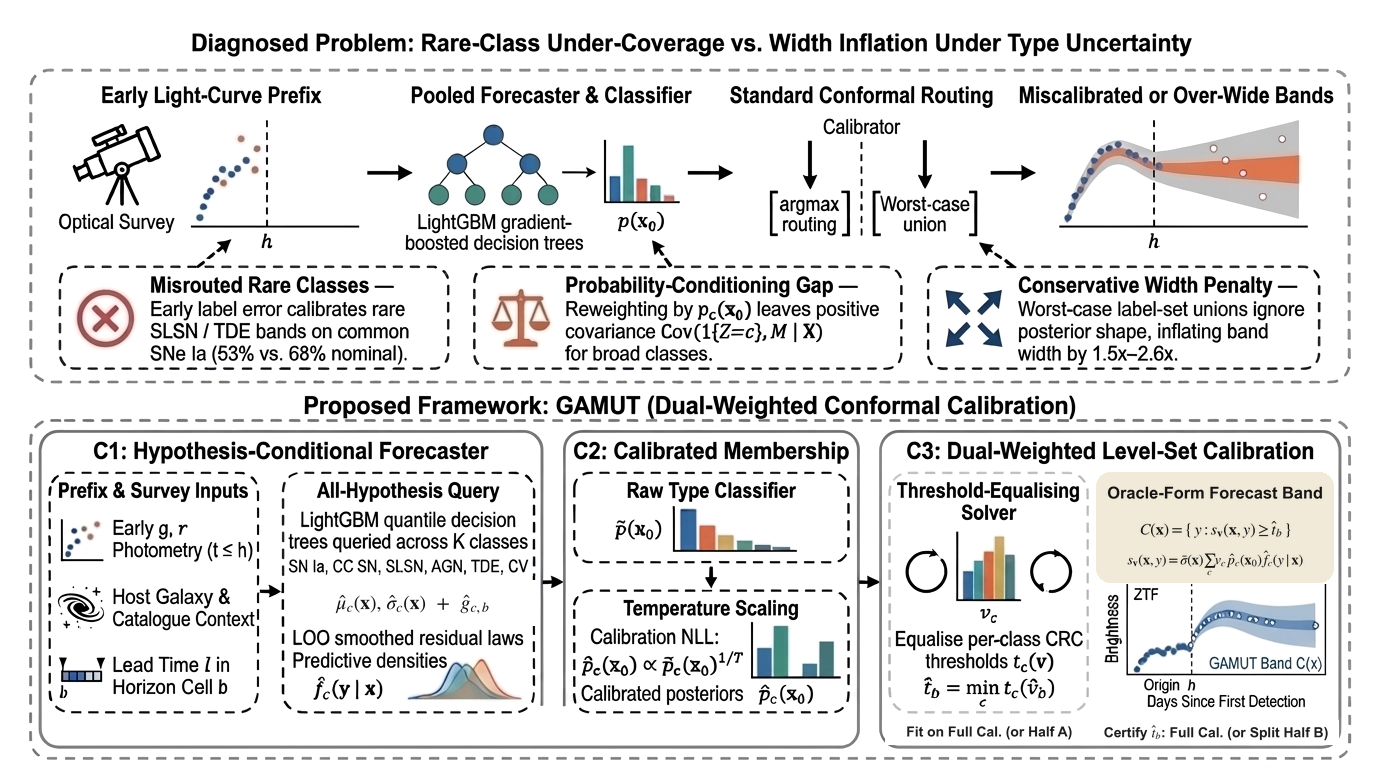
\includegraphics[width=0.97\textwidth]{figures/gamut_framework.png}
\vspace{-4pt}
\caption{Overview of \gamut{} and calibration failure modes under latent type uncertainty. \textbf{Top:} Routing multipliers by the early argmax class under-covers misclassified rare transients, probability reweighting leaves a positive covariance gap (\cref{prop:gap}), and worst-case unions inflate band width across common sources. \textbf{Bottom:} \gamut{} queries a shared hypothesis-conditional quantile forecaster and leave-one-object-out residual laws across all $K$ classes (\textbf{C1}), temperature-scales raw type posteriors (\textbf{C2}), and solves a multiplicative fixed point to equalise per-class conformal risk-control thresholds (\textbf{C3}), outputting level-set bands $C(x)$. Curves and icons are schematic.}
\label{fig:gamut-overview}
\vspace{-4pt}
\end{figure*}

While FLARE's bands achieve nominal marginal coverage across the SN~Ia-dominated stream, they systematically under-cover the rare classes most valuable for follow-up: five days after first detection, the 68\% band contains only \ZTFflareSLSNsixtyeight{} of future SLSN measurements, alongside substantial shortfalls for TDEs and CVs (\cref{fig:observation}).
The cause is structural: routing conformal multipliers by the \emph{predicted} class calibrates misclassified rare transients against common-supernova residuals.
The same mismatch arises across clinical subtyping, regime monitoring, and multi-source sensing whenever calibration data carry ground-truth group labels that remain latent at test time.

Existing remedies force a choice between rare-class under-coverage and excessive width (\cref{fig:gamut-overview}, top).
Conditioning on classifier \emph{probabilities}---via conditional-guarantee conformal prediction \citep{gibbs2025conformal}, posterior localisation \citep{guan2023localized}, or label-shift mixtures \citep{podkopaev2021distribution}---controls a probability-weighted moment rather than true-class coverage.
By \cref{prop:gap}, the two differ by the conditional covariance between class membership and miscoverage plus posterior error; whenever a rare class exhibits broader forecast residuals than the classes with which it is confused, this covariance is positive and sustains under-coverage.
Conversely, latent-class-valid constructions---the max-class quantile \citep{barber2021limits}, two-step label-set unions \citep{timans2024adaptive}, and multi-distribution CP \citep[MDCP;][]{yang2026multi}---ignore or coarsen posterior shape, inflating widths by $1.5\times$--$2.6\times$.

To resolve this tension, we derive the population-optimal band (\cref{prop:oracle}): the set of minimal scale-weighted length satisfying per-class coverage constraints is a superlevel set of $\bar\sigma(x)\sum_c v_c\,p_c(x)f_c(y\mid x)$, with posterior $p_c(x)$, class-$c$ predictive density $f_c(y\mid x)$, posterior-mean scale $\bar\sigma(x)$, and dual weights $v_c$ up-weighting hard-to-cover classes.
\gamut{} (\emph{Guarantees for All Members Under Type uncertainty}; \cref{fig:gamut-overview}, bottom) estimates this oracle via three modules:
\begin{itemize}\setlength{\itemsep}{1pt}\setlength{\parskip}{0pt}\setlength{\topsep}{2pt}
\item[\textbf{C1}] \textbf{Hypothesis-conditional forecaster:} shared LightGBM quantile trees queried across all $K$ hypotheses paired with leave-one-object-out smoothed residual laws $\hat f_c(y\mid x)$, letting rare classes borrow cadence and colour structure from common ones;
\item[\textbf{C2}] \textbf{Calibrated membership posterior:} temperature-scaled probabilities $\hat p_c(x_0)$ fitted on calibration labels;
\item[\textbf{C3}] \textbf{Dual-weighted level-set calibration:} a multiplicative fixed point adjusting $v_c$ to equalise per-class conformal risk-control thresholds across adaptive horizon cells, keeping the minimum eligible threshold.
\end{itemize}
Under FLARE's cross-conformal protocol, \gamut{} reuses out-of-fold calibration data to approximate the oracle empirically.
Under a strict train/calibration/test split reserving a disjoint calibration half for threshold certification (\cref{thm:valid}), the identical rule guarantees finite-sample coverage for every class--horizon cell with sufficient certification objects, regardless of posterior or density misspecification.

\paragraph{Contributions.}
(i) An exact coverage-gap decomposition showing why predicted-class and probability-conditioned calibration under-cover hard rare classes (\cref{prop:gap}), validated on ZTF-BTS.
(ii) Characterisation of the shortest scale-weighted class-valid band (\cref{prop:oracle}), the \gamut{} estimator (\cref{alg:gamut}), and its strict-split finite-sample guarantee (\cref{thm:valid}).
(iii) Evaluation across ZTF-BTS, PLAsTiCC, three UCR archives, a synthetic suite, a strict ZTF split, and two pre-registered untouched PLAsTiCC WFD chunks against 13 baselines: on ZTF, conservative valid baselines are \ZTFValidOverFlareSixtyeight{} (68\%) and \ZTFValidOverFlareNinetyfive{} (95\%) wider than FLARE, whereas \gamut{} achieves class validity at \ZTFWidthRatioSixtyeight{} and \ZTFWidthRatioNinetyfive{} times FLARE's width (\StrictWidthGamutSixtyeight{} and \StrictWidthGamutNinetyfive{} under the strict split) and is \SynValidOverGamutSixtyeight{} (68\%) and \SynValidOverGamutNinetyfive{} (95\%) narrower than valid baselines on synthetic data.
(iv) A learned next-detection simulation with Venn--Abers recalibration that sharpens FLARE's set-closure probabilities.

\section{Problem and Observation}
\label{sec:setup}

\paragraph{Setting.}
An object has a prefix $x_0$ (the light curve up to the forecast origin, summarised as features) and a latent class $Z\in[K]$.
It has future measurements $Y_j$ at lead times $\ell_j$, $j=1,\dots,m$.
Lead times are grouped into horizon cells $b$: unions of contiguous bins of FLARE's lead-time grid, whose finest choice is the grid itself (\cref{sec:method} merges bins only when data are scarce).
A band $C(x)$ is issued for each future point, with $x=(x_0,\ell)$.
Objects are the exchangeable units, so we measure coverage per object and per horizon cell.
Let $m_b$ be the number of the object's points in cell $b$.
The \emph{class-$c$ coverage in cell $b$} is
\begin{equation}
\label{eq:target}
\begin{split}
\cov_{c,b}(C) \coloneqq \E\Big[&\tfrac{1}{m_b}\textstyle\sum_{j:\,b(\ell_j)=b}\one\{Y_j\in C(x_j)\}\\
&\Big|\, Z=c,\ m_b\ge1\Big].
\end{split}
\end{equation}
We want $\cov_{c,b}\ge 1-\alpha$ for every class and every horizon cell.
FLARE reports the per-class coverage pooled over points and bins; we report both.
For cell $b$, let $Q_b$ be the law of $(X,Z,Y)$ obtained by drawing an object with $m_b\ge1$ and then one of its cell-$b$ points uniformly at random.
Then $\cov_{c,b}=Q_b(Y\in C(X)\mid Z=c)$.
Under $Q_b$ we write $p_c(x)=Q_b(Z=c\mid X=x)$, $\pi_{c,b}=Q_b(Z=c)$ and $f_c(y\mid x)$ for the density of $Y$ given $X=x,Z=c$.
The calibration set holds $n$ objects whose \emph{true} classes are known, for example from spectroscopy.
At test time only a classifier's posterior $\hat p(x_0)\in\Delta_K$ is available.

\paragraph{Why calibration on the predicted class or the probabilities fails.}
For any band let $M=\one\{Y\notin C(X)\}$.
Let $m(x)=\P(M=1\mid X=x)$ and $m_c(x)=\P(M=1\mid X=x,Z=c)$, under any of the laws $Q_b$.
\begin{proposition}[coverage gap]
\label{prop:gap}
For every band $C$ and class $c$,
\begin{equation}
\label{eq:gap}
\begin{split}
\P(M=1\mid Z=c) \;=\;& \frac{\E[p_c(X)\,M]}{\pi_c}\\
&+ \frac{\E\big[\Cov(\one\{Z=c\},M\mid X)\big]}{\pi_c},
\end{split}
\end{equation}
where $\Cov(\one\{Z=c\},M\mid X)=p_c(X)\{m_c(X)-m(X)\}$.
Consider a calibration that enforces $\E[\hat p_c(X)(M-\alpha)]=0$ under the same law.
An idealised example is the randomised conditional-guarantee method of \citet{gibbs2025conformal}, applied with objects as units and $\hat p_c$ in its function class.
For such a calibration the class-$c$ miscoverage is
\begin{multline*}
\alpha+\big\{\E[\Cov(\one\{Z=c\},M\mid X)]\\
+\E[(p_c-\hat p_c)(X)(M-\alpha)]\big\}/\pi_c .
\end{multline*}
For Mondrian calibration by the predicted class $L$ with exact cells, the miscoverage is $\alpha+\E[\Cov(\one\{Z=c\},M\mid L)]/\pi_c-\sum_k\P(L=k\mid Z=c)\,\varepsilon_k$, where $\varepsilon_k\in[0,1/(n_k+1)]$ is each cell's conformal slack.
\end{proposition}
The proof is two lines (\cref{app:proofs}).
Because $m=\sum_l p_l m_l$, the covariance is positive, and hence adds miscoverage, when at the same input class $c$ is harder to cover than the classes it is confused with.
This happens to rare classes with broad, heterogeneous light curves, as the class laws $f_c$ there are wider than the others.
A better classifier shrinks the covariance only by separating the classes.
Methods whose weights also depend on $y$ escape the covariance term.
One example is Kandinsky conformal prediction with weights $\P(Z=c\mid X,Y)$ \citep{bairaktari2025kandinsky}, which needs that posterior to be correct.

\paragraph{Observation on ZTF.}
\label{sec:observation}
\Cref{fig:observation} shows our re-implementation of FLARE's bands on its public Bright Transient Survey benchmark (\cref{sec:exp}). It uses the same features, folds and calibration cells; \cref{app:protocol} lists the differences.
At every origin the marginal coverage is within \ZTFflareMargDev{} of nominal.
The SLSN coverage is \ZTFflareSLSNsixtyeight{} at day 5.
Misclassified objects are covered at \ZTFflareMisclsSixtyeight{}, against \ZTFflareCorrectSixtyeight{} for correctly classified ones.
Calibrating on the probabilities instead of the decision raises the worst-class coverage by at most \ZTFprobGainMax{} across the five probability-conditioned methods (\cref{app:observation}).
This is what \cref{prop:gap} leads one to expect.
On synthetic data, where the true laws are known, \cref{eq:gap} reproduces the measured class coverage of the single-interval methods to within \SynPropGapErr{} (\cref{app:synthetic}). These are FLARE, split CP, CQR, GCC, the label-shift mixture and localised CP.

\begin{figure}[t]
\centering
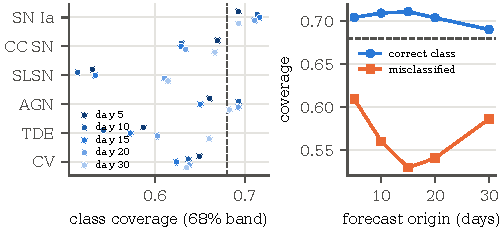
\includegraphics[width=\columnwidth]{figures/observation.pdf}
\caption{FLARE's 68\% bands on ZTF-BTS. Left: per-class coverage at each forecast origin. Right: coverage of correctly and incorrectly classified objects. Dashed: nominal.}
\label{fig:observation}
\end{figure}

\section{Methodology: The \gamut{} Framework}
\label{sec:method}

Given prefix features $x_0$ and lead time $\ell$ in cell $b$, \gamut{} queries a shared hypothesis-conditional forecaster across all $K$ classes to obtain densities $\hat f_c(y\mid x)$ (\textbf{C1}), calibrates membership probabilities $\hat p_c(x_0)$ via temperature scaling (\textbf{C2}), and thresholds $s_v(x,y)=\bar\sigma(x)\sum_c v_c\hat p_c(x_0)\hat f_c(y\mid x)$ using dual multipliers $v_c$ that equalise per-class conformal risk-control thresholds (\textbf{C3}; \cref{fig:gamut-overview,alg:gamut}).

\subsection{Oracle Level-Set Characterisation}
\label{sec:oracle}
To accommodate heteroscedasticity across brightness and horizon, we weight band length by $\omega(x)>0$ (with $\omega=1/\bar\sigma$ below) and relax $C(x)$ to an inclusion rule $I(x,y)\in[0,1]$.

\begin{proposition}[Oracle class-valid forecast band]
\label{prop:oracle}
Fix a cell $b$ with $\pi_{c,b}>0$ for all $c\in[K]$, and assume $Y$ has Lebesgue density $f_c(\cdot\mid x)$ given $(X=x,Z=c)$.
If $\min_C \E_{Q_b}[\omega(X)\,|C(X)|]$ subject to $Q_b(Y\in C(X)\mid Z=c)\ge1-\alpha$ ($\forall c$) admits a feasible band of finite weighted length covering every class strictly above $1-\alpha$, an optimal band is
\begin{equation}
\label{eq:oracle}
C^\star(x)=\Big\{y\in\R:\ \tfrac{1}{\omega(x)}\textstyle\sum_{c=1}^K v^\star_{c}\,p_c(x)\,f_c(y\mid x)\ \ge 1\Big\}
\end{equation}
up to randomisation on $\{\sum_c v^\star_c p_c f_c=\omega\}$, where $v^\star_c=\lambda^\star_c/\pi_{c,b}$, $\lambda^\star\in\R_+^K$ maximises $(1-\alpha)\sum_c\lambda_c-\E_{Q_b}\!\int(\sum_c\tfrac{\lambda_c}{\pi_{c,b}}p_c f_c-\omega)_+dy$, and every class with $v^\star_c>0$ is covered at $1-\alpha$.
\end{proposition}

Three properties guide \gamut{}:
(a) \emph{Scalar cell weights:} Whereas MDCP learns $x$-dependent multipliers, our marginal class programme needs only $K$ scalars $v_c$ per cell; Bayes' rule identifies MDCP's abstract density ratios \citep[Thm.~7]{yang2026multi} as $p_c(x)/\pi_{c,b}$, supplied by a class posterior as in classification \citep{sadinle2019least}.
(b) \emph{HPD interpolation:} Constant $v_c$ recovers the shortest marginally valid weighted level set \citep{lei2013distribution,lei2014distribution}, while larger $v_c$ selectively expands coverage for class $c$.
(c) \emph{Dominance over unions:} Class-wise unions or maxima are primal-feasible and hence no shorter in weighted length than $C^\star$.
With $\omega=1/\bar\sigma$ and $\bar\sigma(x)=\sum_c p_c(x)\sigma_c(x)$, $K=1$ under symmetric unimodal residuals recovers FLARE's normalised-residual band \citep{lei2018distribution}.

\begin{remark}[Scale-weighted length]
\label{rem:abs}
Setting $\omega\equiv1$ thresholds raw density at one bin-wide constant, concentrating coverage on sharp forecasts while abandoning uncertain objects.
Omitting $\bar\sigma$ shortens unweighted length by 2--16\% while trading coverage across objects and horizons (\cref{app:ablation}); we retain $\omega=1/\bar\sigma$ for even forecast adaptivity.
\end{remark}

\subsection{Three-Component Estimator (C1--C3)}
\label{sec:c3}
\paragraph{C1: Hypothesis-conditional forecaster.}
We train three shared LightGBM models (median and 16\%/84\% quantiles) using FLARE's features augmented with the one-hot true class.
Querying them under each hypothesis $c\in[K]$ gives $\hat\mu_c(x)$ and $\hat\sigma_c(x)=\max\{(\hat q_{84,c}-\hat q_{16,c})/2,\sigma_{\min}\}$, letting small classes borrow cadence, colour, and lead-time splits from abundant ones.
On out-of-fold calibration predictions, we estimate per $(c,b)$ the density $\hat g_{c,b}$ of $(y-\hat\mu_c)/\hat\sigma_c$ via a Gaussian-smoothed histogram on $[-60,60]$ with bandwidth twice Silverman's rule (validation-selected; \cref{app:hyper}), pooling bins of class $c$ with $<150$ points to obtain $\hat f_c(y\mid x)=\hat g_{c,b}((y-\hat\mu_c)/\hat\sigma_c)/\hat\sigma_c$.
When scoring a calibration point under its own true class, all points of that object are held out of $\hat g_{c,b}$, preventing self-kernel density inflation.

\paragraph{C2: Calibrated membership posterior.}
Because \cref{eq:oracle} uses $p_c$ as a likelihood-ratio weight, we temperature-scale raw classifier probabilities \citep{guo2017calibration}: $\hat p_c(x_0)\propto \tilde p_c(x_0)^{1/T}$, fitting $T>0$ by calibration NLL.
Although the classifier targets $\P(Z=c\mid x_0)$ whereas $Q_b(Z=c\mid x)$ also conditions on observing a point in cell $b$, multiplicative observation-rate factors $a_{c,b}$ are absorbed into $v_c$ up to input normalisation; residual approximation error affects width but never compromises strict-split validity (\cref{thm:valid}).

\paragraph{C3: Dual-weighted level-set calibration.}
Let $s_v(x,y)=\bar\sigma(x)\sum_c v_c\hat p_c(x_0)\hat f_c(y\mid x)$ and let $L_i(t)$ be the fraction of object $i$'s cell-$b$ points missed by $\{y:s_v(x,y)\ge t\}$.
Per-class conformal risk control \citep{angelopoulos2024conformal} sets
\begin{equation}
\label{eq:crc}
t_{c}(v)=\sup\Big\{t\in\R:\ \textstyle\sum_{i:z_i=c}L_i(t)\le \alpha(n_{c}+1)-1\Big\}
\end{equation}
over the $n_c$ class-$c$ calibration objects in cell $b$.
Using only calibration labels and lead times, we merge adjacent bins until every class with $\ge\lceil2/\alpha\rceil$ calibration objects overall has $\ge\lceil2/\alpha\rceil$ per cell---retaining 6--10 of ZTF's 10 bins at 68\% (2--7 at 95\%), all 6 UCR bins, and 4--9 PLAsTiCC cells at 68\% (1--2 at 95\%, yielding horizon-pooled class validity; \cref{app:cert}).
The cell threshold is $\hat t_b=\min_c t_c(v)$ over eligible classes with $n_c\ge 1/\alpha-1$.
To prevent a single class from pulling $\hat t_b$ down, we equalise $t_c(v)$ via the damped multiplicative fixed point
\begin{equation}
\label{eq:dual}
v_c\leftarrow v_c\cdot\mathrm{clip}\big((\bar t/t_c(v))^{1/2},\tfrac12,2\big),
\end{equation}
with $\bar t$ the geometric mean of included $t_c(v)$ and $v$ renormalised to unit geometric mean, starting from $v_c=1/\hat\pi_c$ and stopping at $\max_c|\log(t_c/\bar t)|<0.005$ or 100 steps.
This heuristic requires a median of \DualItersMedian{} iterations per cell, hitting the cap in \DualItersCapPct{} of cells (\DualItersCapSmall{} on PLAsTiCC-train and ECG5000 at 95\% as slack weights decay toward zero).
Coverage uses exact scores $s_{\hat v_b}(x,y)$, while band length is integrated on a shared grid (400 uniform points across $\pm8\hat\sigma_c$ for $\hat p_c\ge10^{-3}$ plus 49 points within $\pm3\hat\sigma_c$ per hypothesis, shared with Kandinsky CP and MDCP); empty calibration cells borrow the nearest cell's $(\hat v_b,\hat t_b)$.
Calibration and inference take \RuntimeGamutZTF{}s per ZTF fold (\cref{alg:gamut,app:runtime}).

\begin{algorithm}[t]
\caption{\gamut{} Calibration and Prediction}
\label{alg:gamut}
\begin{algorithmic}[1]
\REQUIRE Calibration objects with labels $z_i$; forecasts $\hat\mu_c,\hat\sigma_c$ (\textbf{C1}); raw posteriors $\tilde p$; level $\alpha$
\STATE Fit $T\gets\argmin_T \text{NLL}(\tilde p^{1/T}, z)$; normalise $\hat p\propto \tilde p^{1/T}$ \hfill (\textbf{C2})
\STATE Fit residual laws $\hat g_{c,b}$; score calibration points leave-one-object-out \hfill (\textbf{C1})
\STATE Merge adjacent bins until classes with $\ge\lceil2/\alpha\rceil$ objects overall have $\ge\lceil2/\alpha\rceil$ per cell
\FOR{each horizon cell $b$}
\STATE Set $v\gets 1/\hat\pi$; iterate \cref{eq:dual} until $\max_c|\log(t_c/\bar t)|<0.005$ or 100 steps \hfill (\textbf{C3})
\STATE Set $\hat t_b\gets\min_c t_c(v)$ over classes with $n_{c,b}\ge1/\alpha-1$; store $\hat v_b\gets v$
\ENDFOR
\STATE \textbf{Predict:} $C(x)=\big\{y:\bar\sigma(x)\sum_c \hat v_{b(x),c}\,\hat p_c(x_0)\hat f_c(y\mid x)\ge \hat t_{b(x)}\big\}$
\end{algorithmic}
\end{algorithm}

\subsection{Finite-Sample Guarantees and Operating Protocols}
\label{sec:theory}

\begin{theorem}[Finite-sample per-class validity under strict split]
\label{thm:valid}
Assume base classifiers and forecasters are trained disjointly from calibration and test objects, and calibration and test objects are exchangeable within each true class.
Split calibration objects by stratified halves into $A$ and $B$: on $A$, fit $T$, $\hat\pi$, $\hat g_{c,b}$ (bandwidth and pooling included), merged cells, and weights $\hat v_b$; on $B$, compute $t_c(\hat v_b)$ via \cref{eq:crc} and $\hat t_b=\min_c t_c(\hat v_b)$ over classes with $n^B_{c,b}\ge 1/\alpha-1$.
Conditional on $A$ and on the class labels and cell memberships of $B$, every class $c$ with $n^B_{c,b}\ge1/\alpha-1$ satisfies $\cov_{c,b}(C)\ge1-\alpha$ in every cell $b$ populated in $B$.
\end{theorem}

The proof (\cref{app:proofs}) pairs conformal risk control on $B$ with monotonicity of $L_i(t)$ in $t$.
Validity requires only accurate calibration labels and $n^B_{c,b}\ge1/\alpha-1$; misspecified $\hat p_c$ or $\hat f_c$ affects only width, unlike Kandinsky CP's reliance on exact $\P(Z\mid X,Y)$.
Default \gamut{} uses all out-of-fold calibration objects under FLARE's cross-conformal protocol---where overlapping base-model folds preclude exact finite-sample guarantees for every method \citep{barber2021predictive} and in-sample VC bounds (\cref{app:proofs}) are loose---and is validated empirically; \emph{\gamut{} (strict split)} executes the exact three-way + $A/B$ protocol of \cref{thm:valid} (\cref{app:cert}).

\section{Experiments}
\label{sec:exp}

\subsection{Experimental Setup}
\paragraph{Benchmarks.}
\emph{ZTF-BTS} is FLARE's public Bright Transient Survey benchmark \citep{fremling2020bts,perley2020bts,sasli2026forecast,sasli2026flare} (10,492 spectroscopically classified transients with future targets across six classes), evaluated using FLARE's prefix-causal features, relative $g$/$r$ magnitude targets up to 90 days, five origins ($5,10,15,20,30$d), and five stratified folds.
\emph{PLAsTiCC-train} (2,045 objects, 11 classes) and \emph{PLAsTiCC-DDF} (8,681 chunk-01 deep-drilling objects, 9 classes) come from the unblinded LSST simulation \citep{kessler2019models,hlozek2023results} at origins $5,15,30$d.
Three UCR archives \citep{dau2019ucr}---StarLightCurves (9,236, 3 classes), ECG5000 (5,000, 5 classes, smallest 24), and ElectricDevices (16,637, 7 classes)---are forecast from $20\%,40\%,60\%$ prefixes (\cref{tab:bench}), with UCR Wafer (20\%) and a synthetic suite in the appendix.
Main experiments follow FLARE's five-fold cross-conformal protocol, calibrating on four out-of-fold sets and pooling test predictions across all five folds.

\paragraph{Models and Baselines.}
Every method shares identical cross-fitted classifiers (FLARE's hierarchical model on ZTF; class-weighted LightGBM elsewhere) and LightGBM quantile forecasters \citep{ke2017lightgbm} (\cref{app:protocol}), isolating conformal calibration.
We evaluate 13 external baselines across four families (\cref{app:baselines}):
\emph{Deployed:} FLARE's predicted-class Mondrian bands \citep{sasli2026forecast,sasli2026flare};
\emph{Membership-blind:} normalised-residual split CP \citep{lei2018distribution}, CQR \citep{romano2019conformalized}, and DCP \citep{chernozhukov2021distributional};
\emph{Probability-conditioned:} Localized CP \citep{guan2023localized}, label-shift mixture \citep{podkopaev2021distribution}, GCC \citep{gibbs2025conformal}, learned-partition CP \citep{kiyani2024conformal}, and CPTC \citep{sun2025conformal};
\emph{Latent-class-valid:} two-step CP \citep{timans2024adaptive}, Kandinsky CP \citep{bairaktari2025kandinsky}, MDCP \citep{yang2026multi}, and max-class CP \citep{barber2021limits}.
CPTC, Kandinsky CP, and MDCP use our \textbf{C1} forecaster; we also test \emph{+\,C1} variants of two-step, MDCP, and max-class CP, plus an oracle \emph{True-class Mondrian} reference.

\paragraph{Metrics.}
We report point-pooled class coverage, object-level per-(class, bin) coverage (\cref{eq:target}), worst-class coverage, $\mathrm{CCG}=\frac1K\sum_c|\mathrm{cov}_c-(1-\alpha)|$, and mean width relative to FLARE.
A setting is \emph{valid} if every class's 95\% object-level bootstrap upper bound (500 resamples) reaches $1-\alpha$.
Our initial plan (\cref{app:plan}) pre-registered a fixed worst-class tolerance ($\ge$ nominal $-0.02$/$-0.015$; \cref{app:results}) and class-averaged interval score \citep[IS;][]{gneiting2007strictly}: on IS, \gamut{} ranks first among all valid methods in \ISWinsGamutSixtyeight{} (68\%) and \ISWinsGamutNinetyfive{} (95\%) settings, while beating each always-valid baseline in paired bootstrap tests far more often than losing (two-step \ISVsTwoStepGamutSixtyeight{}, \ISVsTwoStepGamutNinetyfive{}; max-class \ISVsMaxClassGamutSixtyeight{}, \ISVsMaxClassGamutNinetyfive{}; MDCP \ISVsMDGamutSixtyeight{}, \ISVsMDGamutNinetyfive{}; \cref{app:unfavourable}). Main tables report width, matching \cref{prop:oracle}.

\subsection{Main Quantitative Comparison}
\begin{table*}[t]
\centering
\caption{Aggregate performance across the six main benchmarks and all forecast origins (20 settings per nominal level). \emph{Valid}: percentage of settings with no significantly under-covered class (95\% object-level bootstrap upper bound $\ge 1-\alpha$). \emph{Worst}: mean worst-class coverage across settings. \emph{CCG}: mean absolute class-coverage gap. \emph{Cells}: mean number of significantly under-covered (class, lead-time bin) cells per setting. \emph{Width}: mean band length relative to deployed FLARE. Rows are grouped into deployed/membership-blind, probability-conditioned, latent-class-valid, controlled \emph{+\,C1} variants, and \gamut{}. Boldface highlights the best metric among methods achieving $\ge90\%$ empirical class validity at that level. Under this cross-fitted protocol, \emph{\gamut{} (split calibration)} is empirical; formal finite-sample certification requires the strict split in \cref{tab:strictsum,tab:strict}.}
\label{tab:main}
\small
\setlength{\tabcolsep}{5pt}
\resizebox{\linewidth}{!}{%
\begin{tabular}{lccccc@{\hspace{12pt}}ccccc}
\toprule
 & \multicolumn{5}{c}{68\% bands} & \multicolumn{5}{c}{95\% bands} \\
\cmidrule(lr){2-6} \cmidrule(lr){7-11}
Method & Valid (\%) $\uparrow$ & Worst $\uparrow$ & CCG $\downarrow$ & Cells $\downarrow$ & Width $\downarrow$ & Valid (\%) $\uparrow$ & Worst $\uparrow$ & CCG $\downarrow$ & Cells $\downarrow$ & Width $\downarrow$ \\
\midrule
FLARE & 5 & 0.556 & 0.042 & 10.2 & 1.00 & 10 & 0.879 & 0.021 & 7.0 & 1.00 \\
Split CP & 5 & 0.519 & 0.074 & 14.8 & 0.95 & 5 & 0.870 & 0.029 & 11.9 & 0.95 \\
CQR & 5 & 0.515 & 0.079 & 20.5 & 1.01 & 0 & 0.851 & 0.039 & 14.6 & 0.93 \\
DCP & 0 & 0.532 & 0.069 & 17.1 & 1.07 & 0 & 0.880 & 0.026 & 10.3 & 1.11 \\
\midrule
Localized CP & 10 & 0.534 & 0.065 & 13.2 & 0.96 & 5 & 0.876 & 0.026 & 9.8 & 0.96 \\
Label-shift mixture & 30 & 0.575 & 0.037 & 6.5 & 1.01 & 30 & 0.894 & 0.017 & 5.0 & 1.00 \\
GCC ($p$) & 20 & 0.563 & 0.042 & 11.9 & 1.00 & 15 & 0.879 & 0.021 & 8.9 & 0.98 \\
Learned partition & 30 & 0.563 & 0.039 & 9.2 & 1.01 & 25 & 0.883 & 0.020 & 6.8 & 1.00 \\
CPTC & 35 & 0.585 & 0.038 & 5.8 & 1.01 & 80 & 0.922 & 0.017 & 1.1 & 1.17 \\
\midrule
Two-step CP & \textbf{100} & 0.700 & 0.104 & \textbf{0.0} & 1.48 & \textbf{100} & 0.956 & 0.025 & \textbf{0.0} & 1.84 \\
Kandinsky CP & 70 & 0.615 & 0.021 & 7.5 & 1.07 & 55 & 0.917 & 0.010 & 4.8 & 1.10 \\
MDCP & \textbf{100} & 0.705 & 0.130 & 1.8 & 1.62 & \textbf{100} & 0.948 & 0.028 & 1.9 & 1.49 \\
Max-class CP & \textbf{100} & 0.704 & 0.121 & \textbf{0.0} & 1.55 & \textbf{100} & 0.958 & 0.030 & \textbf{0.0} & 2.61 \\
\midrule
Two-step CP + C1 & \textbf{100} & 0.734 & 0.135 & \textbf{0.0} & 1.70 & \textbf{100} & 0.962 & 0.029 & \textbf{0.0} & 1.75 \\
MDCP + C1 & \textbf{100} & 0.702 & 0.141 & 2.5 & 1.73 & \textbf{100} & 0.949 & 0.030 & 1.6 & 1.54 \\
Max-class CP + C1 & \textbf{100} & \textbf{0.751} & 0.174 & \textbf{0.0} & 1.96 & \textbf{100} & \textbf{0.968} & 0.036 & \textbf{0.0} & 2.22 \\
\midrule
\rowcolor{gray!12}\gamut{} (ours) & \textbf{100} & 0.671 & \textbf{0.014} & 0.2 & \textbf{1.09} & 90 & 0.949 & \textbf{0.012} & 0.8 & \textbf{1.36} \\
\gamut{} (split calibration) & \textbf{100} & 0.745 & 0.096 & \textbf{0.0} & 1.47 & \textbf{100} & \textbf{0.968} & 0.028 & 0.1 & 1.62 \\
\textcolor{gray}{True-class Mondrian (reference)} & 85 & 0.633 & 0.008 & 1.6 & 1.00 & 90 & 0.926 & 0.004 & 0.2 & 1.02 \\
\bottomrule
\end{tabular}}
\end{table*}


Across all 20 benchmark--origin settings (\cref{tab:main}), membership-blind and probability-conditioned methods maintain marginal coverage but fail on rare classes: at 68\%, none exceeds \MainValidBestNonValidSixtyeight{} validity, confirming \cref{prop:gap}.
Two-step, MDCP, and max-class CP reach 100\% validity by over-covering common classes (68\% CCG \MainCCGValidBaselinesSixtyeight{}), inflating widths to \MainWidthValidBaselinesSixtyeight{} (68\%) and \MainWidthValidBaselinesNinetyfive{} (95\%) times FLARE's (\MainWidthCOneBaselinesSixtyeight{} and \MainWidthCOneBaselinesNinetyfive{} with \emph{+\,C1}).
\gamut{} attains \MainValidGamutSixtyeight{} validity at 68\% (\MainValidTolGamutSixtyeight{} under fixed tolerance) at width \MainWidthGamutSixtyeight{} and CCG \MainCCGGamutSixtyeight{}---7--9$\times$ tighter around nominal---cutting mean width by \WidthGainValidMean{} versus always-valid baselines (\WidthGainValidSixtyeight{} at 68\%, \WidthGainValidNinetyfive{} at 95\%) and \WidthGainCOneMean{} versus their \emph{+\,C1} variants.
At 95\%, \gamut{} is valid in \MainValidGamutNinetyfive{} of settings (except point-pooled SN~Ia at 0.93 on PLAsTiCC-train); CPTC reaches \MainValidBestNonValidNinetyfive{} at width \MainWidthCPTCNinetyfive{} but only \MainValidCPTCSixtyeight{} at 68\%, while tiny classes (19--40 calibration objects on ECG5000 and PLAsTiCC-train) make \gamut{} wider than MDCP in \NinetyfiveWiderThanMDCP{} of 95\% settings (\cref{app:unfavourable}).
On fine-grained (class, bin) cells (\cref{eq:target}), \gamut{} cuts FLARE's \MainCellsFlareSixtyeight{}/\MainCellsFlareNinetyfive{} under-covered cells to \MainCellsGamutSixtyeight{}/\MainCellsGamutNinetyfive{} (vs.\ \MainCellsMDCPSixtyeight{}/\MainCellsMDCPNinetyfive{} for MDCP and 0.0 for two-step/max-class CP). On \gamut{}'s merged cells, in-sample reuse leaves \MergedGamutSixtyeight{}/\MergedGamutNinetyfive{} sparse PLAsTiCC cells under-covered, whereas split-calibration \gamut{} leaves \MergedCertSixtyeight{}/\MergedCertNinetyfive{} at widths \MainWidthCertSixtyeight{}/\MainWidthCertNinetyfive{}.

\begin{figure*}[t]
\centering
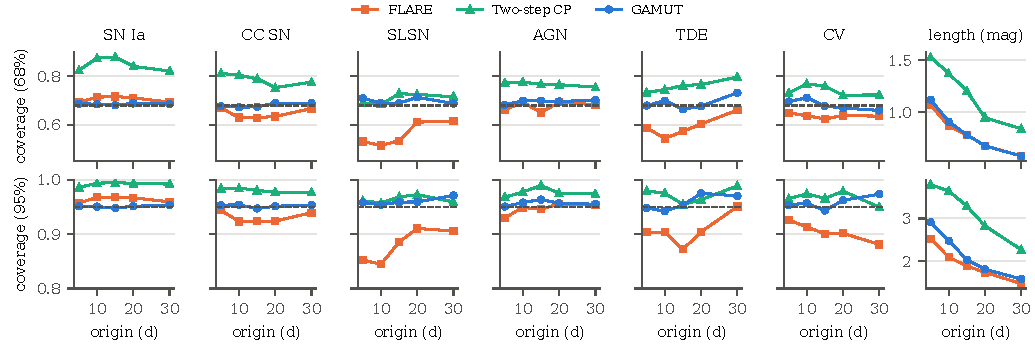
\includegraphics[width=0.92\textwidth]{figures/ztf_classes.pdf}
\vspace{-5pt}
\caption{ZTF-BTS per-class coverage and mean band width across forecast origins at 68\% (top) and 95\% (bottom) for FLARE, two-step CP, and \gamut{}. Dashed lines mark nominal coverage; right panels show mean band length in magnitudes.}
\label{fig:ztf}
\vspace{-4pt}
\end{figure*}

\paragraph{ZTF-BTS and Pre-Registered Held-Out Chunks.}
On ZTF-BTS (\cref{fig:ztf}), FLARE's 68\% SLSN and TDE coverage stays between \ZTFflareSLSNmin{} and \ZTFflareSLSNmax{}, whereas \gamut{} never falls more than \ZTFgamutMaxUnderSixtyeight{} (68\%) or \ZTFgamutMaxUnderNinetyfive{} (95\%) below nominal for any class at any origin at \ZTFWidthRatioSixtyeight{} and \ZTFWidthRatioNinetyfive{} times FLARE's width.
To bound post-inspection tuning (\cref{app:history}), we froze code checksums and ran once on untouched Wide-Fast-Deep transients from PLAsTiCC chunk 02 (20,760 objects, 12 classes; \cref{app:held}): FLARE is 0\% valid (worst class \HeldWorstFlareSixtyeight{} at 68\%), whereas \gamut{} is 100\% valid at all origins and levels at widths \HeldWidthGamutSixtyeight{} (68\%) and \HeldWidthGamutNinetyfive{} (95\%) versus \HeldWidthValidSixtyeight{} and \HeldWidthValidNinetyfive{} for conservative baselines (\HeldCellsGamutNinetyfive{} under-covered 95\% cells vs.\ 0.0 for two-step/max-class CP).
A second untouched WFD chunk 03 (20,475 objects; \cref{app:held}) confirms 100\% validity at widths \HeldBWidthGamutSixtyeight{} and \HeldBWidthGamutNinetyfive{} (FLARE: 0\%).

\subsection{Ablation, Synthetic, Strict-Split, and Closure Studies}
\begin{table}[t]
\centering
\caption{Ablations, aggregated over the six main benchmarks and all origins. Width is relative to full \gamut. Columns as in \cref{tab:main}.}
\label{tab:ablation}
\scriptsize
\setlength{\tabcolsep}{3pt}
\resizebox{\linewidth}{!}{%
\begin{tabular}{lccccc@{\hspace{6pt}}ccccc}
\toprule
 & \multicolumn{5}{c}{68\%} & \multicolumn{5}{c}{95\%} \\
\cmidrule(lr){2-6} \cmidrule(lr){7-11}
Variant & Val. & Worst & CCG & Cells & W. & Val. & Worst & CCG & Cells & W. \\
\midrule
\rowcolor{gray!12}\gamut{} (full) & 100 & 0.671 & 0.014 & 0.2 & 1.00 & 90 & 0.949 & 0.012 & 0.8 & 1.00 \\
\midrule
w/o C1: pooled forecaster & 100 & 0.675 & 0.017 & 0.1 & 1.04 & 85 & 0.952 & 0.015 & 0.7 & 1.03 \\
w/o C2: uniform posterior & 100 & 0.694 & 0.094 & 0.2 & 1.43 & 100 & 0.967 & 0.032 & 0.1 & 1.47 \\
w/o C2: argmax posterior & 100 & 0.698 & 0.089 & 0.0 & 1.38 & 100 & 0.960 & 0.029 & 0.0 & 1.35 \\
w/o C2 calibration (raw $\tilde p$) & 100 & 0.672 & 0.014 & 0.1 & 1.01 & 90 & 0.948 & 0.012 & 0.6 & 1.00 \\
w/o C3: posterior mixture & 0 & 0.516 & 0.068 & 15.1 & 0.86 & 0 & 0.862 & 0.026 & 10.2 & 0.73 \\
w/o C3: prior-ratio weights & 100 & 0.686 & 0.175 & 0.1 & 1.45 & 100 & 0.964 & 0.030 & 0.0 & 1.17 \\
fixed lead bins (no merging) & 100 & 0.671 & 0.015 & 0.1 & 1.01 & 95 & 0.946 & 0.013 & 0.2 & 1.03 \\
\gamut{} (split calibration) & 100 & 0.745 & 0.096 & 0.0 & 1.33 & 100 & 0.968 & 0.028 & 0.1 & 1.29 \\
\bottomrule
\end{tabular}}
\end{table}


\paragraph{Ablations and Synthetic Suite.}
In \cref{tab:ablation}, uniform or argmax posteriors keep validity via \textbf{C3} but widen bands by \AblWidthUniform{} and \AblWidthArgmax{}; dropping \textbf{C3} collapses 68\% validity to \AblValidMixtureSixtyeight{} (worst \AblWorstMixtureSixtyeight{}), and static inverse-prior weights add \AblWidthBalanced{} width.
Dropping \textbf{C1} shifts real-benchmark width by \AblWNoConeSixtyeight{}/\AblWNoConeNinetyfive{} (95\% validity \MainValidGamutNinetyfive{}$\to$\AblValidNoConeNinetyfive{}) where early prefixes look similar across classes, but \textbf{C1} cuts width by \AblConeSynSixtyeight{}/\AblConeSynNinetyfive{} on synthetic data with distinct class trajectories, where \gamut{} approaches the oracle band within \SynOracleGapSixtyeight{}/\SynOracleGapNinetyfive{} versus \SynOracleGapValidSixtyeight{}/\SynOracleGapValidNinetyfive{} for valid baselines (\cref{app:synthetic}).
Temperature scaling changes real width little (\AblWRawSixtyeight{}, \AblValidRawNinetyfive{} valid at 95\%) but saves \AblRawKtwoSixtyeight{}/\AblRawKtwoNinetyfive{} at $\kappa=2$.
Without leave-one-object-out scoring, day-20 ZTF CV coverage drops to \AblWorstNoLooZTF{} (95\% validity \AblValidNoLooNinetyfive{}); one horizon-wide threshold lets a ZTF cell hit \AblOneThreshWorstCell{}; and validation sweeps shift worst-class coverage by $\le$\HyperMaxWorstChange{} and width by $\le$\HyperMaxWidthChange{} aside from 5 dual steps raising ECG5000 CCG from \HyperDualFiveCCGFrom{} to \HyperDualFiveCCGTo{} (\cref{app:hyper}). Fixed bins slightly edge adaptive merging on 95\% test folds (\AblValidFixedBinsNinetyfive{} valid, \AblWFixedBinsSixtyeight{}/\AblWFixedBinsNinetyfive{} width), but we retain validation-chosen merging (\HyperFixedBinsWidthMin{}--\HyperFixedBinsWidthMax{} narrower on validation) and object-level units (\cref{thm:valid}).

\paragraph{Strict Three-Way Split.}
Rotating three base-training folds, one calibration fold, and one test fold on ZTF-BTS satisfies \cref{thm:valid} (\cref{tab:strictsum}, \cref{app:cert}).
Across all \StrictNOrigins{} origins, FLARE is 0\% valid, whereas \gamut{} is 100\% valid at widths \StrictWidthGamutSixtyeight{} (68\%) and \StrictWidthGamutNinetyfive{} (95\%) versus \StrictWidthTwoStepSixtyeight{}--\StrictWidthMDCPSixtyeight{} and \StrictWidthTwoStepNinetyfive{}--\StrictWidthMDCPNinetyfive{} for always-valid baselines.
Certified \emph{\gamut{} (strict split)} achieves 100\% empirical validity at widths \StrictWidthCertSixtyeight{} and \StrictWidthCertNinetyfive{}; at 95\%, full-fold \gamut{} is wider because 19--39-object classes remain active with near-zero risk budget, whereas Half-$B$ size screening ($n^B_{c,b}\ge19$) certifies SN~Ia and CC~SN while excluding SLSN, AGN, TDE, and CV.

\paragraph{Next-Observation Set Closure.}
To predict whether one next-night detection narrows FLARE's 90\% classification set to a singleton, replacing FLARE's argmax-routed fixed-scatter Gaussian draws with \textbf{C1} empirical-residual draws, \textbf{C2} mixing, and inductive Venn--Abers \citep{vovk2014venn} cuts test Brier score by \CloFiveBrierGainVA{} (day 5) and \CloTenBrierGainVA{} (day 10) against Venn--Abers-recalibrated FLARE and lifts AUC (\CloFiveAUCDep{}$\to$\CloFiveAUCOurs{}, \CloTenAUCDep{}$\to$\CloTenAUCOurs{}) at matching ECE (\cref{app:closure}).
Uncalibrated, it meets FLARE's $\pm0.10$ five-bin tolerance in \CloFiveProfOursRaw{} and \CloTenProfOursRaw{} bins versus \CloFiveProfDep{} and \CloTenProfDep{}.
A pooled empirical-residual control gives Brier \CloFiveBrierPooled{} and \CloTenBrierPooled{}, showing that the learned next-point law rather than class mixing drives the gain, while small day-10 SLSN slices remain noisy.

\section{Related Work}
\label{sec:related}

\paragraph{Conditional and Group Conformal Prediction.}
Distribution-free split conformal prediction \citep{papadopoulos2002inductive,vovk2005algorithmic,angelopoulos2023gentle} guarantees marginal coverage, whereas exact covariate-conditional validity is impossible without structural assumptions \citep{vovk2012conditional,barber2021limits}.
Tractable relaxations condition on observed groups or features via Mondrian strata \citep{vovk2005algorithmic}, equalised coverage \citep{romano2020malice}, multivalid calibration \citep{jung2023batch}, moment-class guarantees \citep{gibbs2025conformal}, learned partitions \citep{kiyani2024conformal}, localisation \citep{guan2023localized}, and group-weighted CP \citep{bhattacharyya2024group}, while class-conditional classification sets \citep{sadinle2019least,ding2023class} test candidate labels directly.
Because our target $Y$ is continuous while $Z$ is latent at test time, feature or probability conditioning leaves the covariance gap in \cref{prop:gap}.

\paragraph{Latent Groups and Multi-Source Calibration.}
Kandinsky CP \citep{bairaktari2025kandinsky} weights scores by $\P(Z=c\mid X,Y)$, requiring accurate joint posteriors.
MDCP \citep{yang2026multi} aggregates source $p$-values via max-$p$ unions and learns $x$-dependent multipliers for source-uniform validity at every $x$, leaving open how to exploit estimated membership with finite-sample guarantees---addressed at the per-class level by \cref{prop:oracle,thm:valid}.
Two-step CP \citep{timans2024adaptive} takes worst-case quantiles over conformal label sets, mixture-of-experts sets \citep{javanmard2022prediction} are asymptotic unions, and CPTC \citep{sun2025conformal} pairs state-conditional forecasters (akin to \textbf{C1}) with posterior-truncated unions for marginal coverage, while label-shift \citep{podkopaev2021distribution}, subpopulation-shift \citep{wang2025conformal}, and posterior CP \citep{zhang2024posterior} target marginal or shifted laws rather than per-component validity.

\paragraph{Level Sets and Transient Forecasting.}
Minimum-measure marginal sets are density superlevel sets \citep{lei2013distribution,lei2014distribution}, conformalised by HPD-split \citep{izbicki2022cd} and classification Neyman--Pearson sets \citep{sadinle2019least}; \cref{prop:oracle} extends them to latent-class constraints.
In transient astronomy, per-class models flag anomalies without calibrated bands \citep{muthukrishna2022real}, conformal time-series methods target marginal/online coverage \citep{stankeviciute2021conformal,gibbs2021adaptive}, and FLARE \citep{sasli2026forecast,sasli2026flare} and ASTRANet \citep{sasli2026astranet} stratify by predicted classes or anomaly scores.

\section{Conclusion}
\label{sec:conclusion}

Calibrating by the predicted type or its probabilities can under-cover rare latent types when the class is uncertain at prediction time.
\gamut{} estimates a scale-weighted band from class-conditional forecast distributions, classifier probabilities, and dual-weighted conformal calibration, while \gamut-cert{} supplies a finite-sample guarantee for eligible class--horizon cells under a strict split.
On ZTF, the method substantially improves the rare-class coverage problem in the reported settings, including the strict split and two held-out sets, with bands \MainWidthGamutSixtyeight{} (68\%) and \MainWidthGamutNinetyfive{} (95\%) times FLARE's and shorter bands than the always-valid baselines on average.
The default \gamut{} is an empirical method because it reuses calibration data; the certificate belongs to \gamut-cert{} and depends on having enough certification objects in each eligible cell.
The bands can become wider for very small classes at 95\%, and the closure study's main gain comes from the learned next-point law, while the additional benefit from class conditioning is smaller and not uniform across rare classes.


\section*{Impact Statement}
This work aims to make uncertainty statements reliable for every subpopulation, including rare ones, when the subpopulation of a new case is unknown.
In astronomy it supports the allocation of scarce follow-up time to rare transients.
In other domains with latent types, for example clinical subtypes, the same property guards against systematically over-confident predictions for minority groups.
The class-validity claim is limited by the labels of the calibration set and the chosen taxonomy; the finite-sample certificate also requires the strict split and enough certification objects.
A group missing from the taxonomy, or labelled unreliably, receives no protection.
Practitioners should audit both before relying on per-group coverage. The limitations of the method, including its dependence on the class taxonomy and on the quality of the calibration labels, are listed in \cref{app:limits}.


\section*{Software and Data}
Source code implementing \gamut{}, all thirteen external baselines, the benchmark builders, pre-registration checksums, raw evaluation tables, and end-to-end reproduction scripts is publicly available at \url{https://github.com/appleweiping/GAMUT}. The ZTF Bright Transient Survey photometric classification and forecasting pipeline from FLARE \citep{sasli2026flare,sasli2026forecast} is available at \url{https://github.com/applecider-ml/flare}. The unblinded LSST PLAsTiCC dataset \citep{kessler2019models,hlozek2023results} is archived on Zenodo (\texttt{doi:10.5281/zenodo.2539456}), and the UCR Time Series Archive \citep{dau2019ucr} is publicly available from the UCR repository.

\section*{Acknowledgements}
We thank the FLARE team and the Zwicky Transient Facility (ZTF) Bright Transient Survey collaboration for making their transient photometry, spectroscopic classifications, feature pipelines, and baseline models available \citep{bellm2019ztf,fremling2020bts,perley2020bts,sasli2026flare,sasli2026forecast}. We also acknowledge the LSST Dark Energy Science Collaboration and the PLAsTiCC team for the public transient simulation archive \citep{kessler2019models,hlozek2023results}, and the maintainers of the UCR Time Series Archive \citep{dau2019ucr}.

\bibliography{references}
\bibliographystyle{icml2026}

\newpage
\appendix
\crefalias{section}{appendix}
\crefalias{subsection}{appendix}
\counterwithin{table}{section}
\counterwithin{figure}{section}
\onecolumn
\section{Proofs}
\label{app:proofs}

Throughout, $(X,Z,Y)$ is drawn from one of the laws $Q_b$ of \cref{sec:setup}.
For a band $C$ we write $M=\one\{Y\notin C(X)\}$, $m(x)=\P(M=1\mid X=x)$, $m_c(x)=\P(M=1\mid X=x,Z=c)$ and $p_c(x)=\P(Z=c\mid X=x)$.

\paragraph{Proof of \cref{prop:gap}.}
By the tower property, $\P(M=1,Z=c)=\E[\E(\one\{Z=c\}M\mid X)]=\E[p_c(X)m_c(X)]$ and $\E[p_c(X)M]=\E[p_c(X)m(X)]$.
Subtracting and dividing by $\pi_c$ gives \cref{eq:gap}.
Moreover $\Cov(\one\{Z=c\},M\mid X)=\E[\one\{Z=c\}M\mid X]-p_c(X)m(X)=p_c(X)\{m_c(X)-m(X)\}$.
If a calibration ensures $\E[\hat p_c(X)(M-\alpha)]=0$, then
$\E[p_c(X)M]=\E[\hat p_c(X)M]+\E[(p_c-\hat p_c)(X)M]=\alpha\E[\hat p_c(X)]+\E[(p_c-\hat p_c)(X)M]$.
Since $\E[\hat p_c(X)]=\pi_c-\E[(p_c-\hat p_c)(X)]$, this equals $\alpha\pi_c+\E[(p_c-\hat p_c)(X)(M-\alpha)]$.
Substituting into \cref{eq:gap} gives the stated miscoverage.
The randomised version of the method of \citet{gibbs2025conformal} attains the moment equality exactly for every function in its finite-dimensional class, under the law of its exchangeable units.
Under $Q_b$ the units are objects drawn with one point each.
Point-level, unrandomised or subsampled versions, such as our baseline, attain the equality only approximately.
For Mondrian calibration by the predicted class $L$, apply the same argument with the sub-$\sigma$-algebra $\sigma(L)$ in place of $\sigma(X)$; the weight $\P(Z=c\mid L)$ is a linear combination of the cell indicators.
With exact cells and almost surely distinct scores, each cell's conformal quantile gives $\P(M=1\mid L=k)=\alpha-\varepsilon_k$ with $\varepsilon_k\in[0,1/(n_k+1)]$.
Substituting gives the formula in \cref{prop:gap}.
FLARE's fallback for small cells and its cross-conformal protocol make this only approximate.
\hfill$\square$

\paragraph{Proof of \cref{prop:oracle}.}
Write $\mathrm{cov}_c(I)=\pi_{c,b}^{-1}\E_{Q_b}\!\int I(X,y)\,p_c(X)f_c(y\mid X)\,dy$ for $I:\mathcal X\times\R\to[0,1]$, and $h_\lambda(x,y)=\sum_c(\lambda_c/\pi_{c,b})\,p_c(x)f_c(y\mid x)$.
\emph{Weak duality.} For feasible $I$ and $\lambda\ge0$,
\[
\E\!\int \omega I\,dy \ \ge\ \E\!\int \omega I\,dy-\sum_c\lambda_c\{\mathrm{cov}_c(I)-(1-\alpha)\}
= \E\!\int I(\omega-h_\lambda)\,dy+(1-\alpha)\sum_c\lambda_c \ \ge\ D(\lambda),
\]
where $D(\lambda)=(1-\alpha)\sum_c\lambda_c-\E\!\int(h_\lambda-\omega)_+dy$.
The last step uses $I(\omega-h_\lambda)\ge-(h_\lambda-\omega)_+$ for $I\in[0,1]$.
$D$ is concave as an infimum of affine functions of $\lambda$.
\emph{Existence and strong duality.} The set $\{0\le I\le1\}$ is weak-$^*$ compact in $L^\infty$, and the constraints are weak-$^*$ continuous because $p_cf_c\in L^1$.
The objective is weak-$^*$ lower semicontinuous.
A minimiser therefore exists among the feasible $I$ of finite weighted length, which are assumed to exist.
The programme is linear in $I$, with finitely many constraints and a Slater point (the assumption of the proposition).
Lagrange duality for convex programmes \citep[\S8.6, Thm.~1]{luenberger1969optimization} gives $\lambda^\star\ge0$ with $\min=D(\lambda^\star)$.
\emph{Characterisation.} Both inequalities are equalities iff three conditions hold: $I=1$ on $\{h_{\lambda^\star}>\omega\}$; $I=0$ on $\{h_{\lambda^\star}<\omega\}$; and $\lambda^\star_c\{\mathrm{cov}_c(I)-(1-\alpha)\}=0$ for all $c$.
With $v^\star_c=\lambda^\star_c/\pi_{c,b}$ this is \cref{eq:oracle}.
The solution need not be unique on $\{h_{\lambda^\star}=\omega\}$.
Finally, the union or maximum of class-wise valid bands is feasible, so its weighted length is at least that of $C^\star$.
\hfill$\square$

\paragraph{Proof of \cref{thm:valid}.}
Condition on the base models, on everything computed from $A$ (including the horizon cells), and on the class labels and cell memberships ($m_b\ge1$ or not) of the objects of $B$; the counts $n^B_{c,b}$ are then fixed.
Fix a cell $b$ with calibration points in $B$ and a class $c$ with $n^B_{c,b}\ge1/\alpha-1$.
The score $s_{v_b}$ is then a fixed function.
The losses $L_i(t)$ of the class-$c$ objects of $B$ with points in bin $b$ lie in $[0,1]$.
They are non-decreasing and left-continuous in $t$.
In the parametrisation $\lambda=-t$ they are non-increasing and right-continuous, and $L_i\to0$ as $t\to-\infty$.
These objects and a class-$c$ test object with points in cell $b$ are exchangeable given this conditioning, because nothing used to build the score depends on $B$ or on the test object, and the target \cref{eq:target} conditions on the same event $\{Z=c,\ m_b\ge1\}$.
Conformal risk control \citep[Thm.~1]{angelopoulos2024conformal} with bound $B=1$ therefore gives $\E[L_{n+1}(t_c)]\le\alpha$, with $t_c$ from \cref{eq:crc}.
The budget is non-negative because $n^B_{c,b}\ge1/\alpha-1$.
Since $\hat t_b\le t_c$ and $L_{n+1}$ is non-decreasing, $L_{n+1}(\hat t_b)\le L_{n+1}(t_c)$ pointwise.
Hence $1-\cov_{c,b}=\E[L_{n+1}(\hat t_b)]\le\alpha$, whatever the other classes' thresholds are.
Classes below the size cutoff are excluded from the minimum and receive no guarantee in that bin.
Cells without calibration points in $B$, which borrow a neighbour's threshold, receive none either.
\Cref{app:cert} counts both, and lists the realised cells.
\hfill$\square$

\paragraph{A uniform-convergence bound for in-sample weights.}
Suppose the features $\tilde T(x,y)=\bar\sigma(x)\,(\hat p_c(x)\hat f_c(y\mid x))_{c\le K}$ are fixed, that is, fitted on data independent of the calibration set.
Suppose also that, within a bin, $(v,t)$ is chosen on the calibration objects by any rule with $\hat R_c(v,t)\le\alpha$.
The miss indicators $\one\{\langle v,\tilde T\rangle<t\}$ are affine half-spaces in $\R^K$, so their VC dimension is at most $K+1$.
On $n_c$ i.i.d.\ objects with at most $m_{\max}$ points each, let $N_c=n_cm_{\max}\ge K+1$.
The Sauer--Shelah and Massart lemmas bound the Rademacher complexity of the object-level losses by $\sqrt{2(K+1)\log(eN_c/(K+1))/n_c}$.
With the bounded-differences inequality \citep[Thm.~3.3]{mohri2018foundations} and a union bound over $K$ classes and $J$ cells, with probability at least $1-\delta$ over the calibration data,
\[
\cov_{c,b}\ \ge\ 1-\alpha-2\sqrt{2(K+1)\log\big(eN_c/(K+1)\big)/n_c}-\sqrt{\log(KJ/\delta)/(2n_c)}
\]
for all $c$ and $b$.
Here the cells are fixed in advance; data-dependent merging adds a further union bound over the $2^{9}$ contiguous partitions of FLARE's ten bins.
With $K=6$, $m_{\max}=267$ (the most points of any ZTF object at day 5), $\delta=0.1$ and $J=10$, the slack is about 2.0 at $n_c=150$ and 0.35 at $n_c=7{,}000$, so the bound is uninformative for rare classes.
Moreover the default \gamut{} also fits $T$ and $\hat g$ on the calibration objects, so its features are not fixed.
We state the bound only to show that the in-sample fit of $K$ weights per bin costs $O(\sqrt{K\log N/n})$ in principle; we make no practical claim from it.

\paragraph{The dual fixed point.}
If $t_c(v)=t$ for all included classes, then $\{y:s_v\ge t\}=\{y:s_{v/t}\ge1\}$.
Every included class's calibration constraint \cref{eq:crc} then binds at the same threshold.
If $\hat p$ and $\hat f$ were the true laws, this would be the complementary-slackness pattern of \cref{prop:oracle} with all multipliers positive.
We do not claim more.
The update \cref{eq:dual} is a damped multiplicative rule on threshold ratios, not a gradient step on $D$, and we prove neither its convergence nor the uniqueness of its fixed point.


\FloatBarrier
\section{Benchmarks, Base Models, and Protocol}
\label{app:protocol}
\begin{table}[t]
\centering
\caption{Benchmarks. Objects with at least one future point, and future points, at the earliest origin; \emph{min} is the size of the smallest class.}
\label{tab:bench}
\scriptsize
\setlength{\tabcolsep}{3pt}
\resizebox{\linewidth}{!}{%
\begin{tabular}{llrrrrl}
\toprule
Benchmark & Domain & Objects & $K$ & min & Points & Origins \\
\midrule
ZTF-BTS & ZTF transients & 10,492 & 6 & 68 & 273,908 & 5,10,15,20,30 d \\
PLAsTiCC-train & LSST sim. & 2,045 & 11 & 36 & 21,461 & 5,15,30 d \\
PLAsTiCC-DDF & LSST sim. (DDF) & 8,681 & 9 & 42 & 74,139 & 5,15,30 d \\
StarLight & stellar light curves & 9,236 & 3 & 1329 & 221,664 & 20,40,60\% \\
ECG5000 & ECG & 5,000 & 5 & 24 & 120,000 & 20,40,60\% \\
ElecDevices & electricity & 16,637 & 7 & 1252 & 399,288 & 20,40,60\% \\
Wafer & semiconductor & 7,164 & 2 & 762 & 171,936 & 20\% \\
PLAsTiCC-WFD (held out) & LSST sim. (WFD) & 20,760 & 12 & 30 & 115,532 & 5,15,30 d \\
\bottomrule
\end{tabular}}
\end{table}


\paragraph{ZTF-BTS.}
Objects, spectroscopic class labels, photometry, and host-galaxy catalogue context follow FLARE's public Bright Transient Survey release \citep{sasli2026forecast,sasli2026flare}.
For each forecast origin $h\in\{5,10,15,20,30\}$ days since first detection, inputs consist of FLARE's prefix-causal feature vector computed strictly on detections at $t\le h$, matching FLARE's inference pipeline.
Targets comprise all subsequent $g$- or $r$-band detections in $h<t\le90$ days, expressed in AB magnitudes relative to the brightest prefix detection.
Outer folds match FLARE's exact split (\texttt{StratifiedKFold(5, shuffle=True, random\_state=42)} over the concatenated train/validation/test pool).
FLARE's hierarchical classifier is retrained in every fold using its released recipe to produce uncalibrated probabilities $\tilde p(x_0)$, and FLARE's baseline routes conformal multipliers by $\argmax_c \tilde p_c(x_0)$.
Whereas deployed FLARE switches to a class-weighted point forecaster when the argmax class is rare, all methods here share one pooled base forecaster (and shared \textbf{C1} where applicable) so differences reflect uncertainty calibration alone.

\paragraph{PLAsTiCC.}
From the unblinded LSST PLAsTiCC release \citep{kessler2019models,hlozek2023results}, $g$-, $r$-, and $i$-band detections are mapped to FLARE's event representation (days since first detection and log flux in $\mu$Jy), filtered by FLARE's quality criteria ($\ge8$ detections within 100 days, including at least two in $g$ and two in $r$), and featurised identically to ZTF without external host-catalogue features; classes with fewer than 30 objects are omitted.
\emph{PLAsTiCC-train} uses the spectroscopically selected training set, while \emph{PLAsTiCC-DDF} uses deep-drilling-field events from test chunk 01.

\paragraph{UCR Time-Series Archives.}
Archive training and test splits are pooled with archive class annotations serving as latent types $Z$.
Observing the first $h\in\{20,40,60\}\%$ of each series, we extract a 32-point resampled prefix together with its mean, standard deviation, extrema, terminal value, local slope, curvature, and quartiles; forecast targets are up to 24 uniformly spaced future steps measured relative to the last prefix value.
Because standard UCR releases $z$-normalise series across their full length, future scale information leaks mildly into prefixes \citep{renault2025early} identically for all methods (\cref{app:limits}); on phase-folded StarLightCurves, future steps correspond to later orbital/pulsation phases.

\paragraph{Cross-Fitting Hyperparameters.}
In each outer fold, base classifiers and LightGBM quantile forecasters (127 leaves, minimum child samples 100, feature fraction 0.6, bagging fraction 0.8) are trained on the remaining four folds using an 85/15 object-level split for early stopping.
Within our compute budget, we use learning rate 0.05 and up to 24 subsampled training targets per object on ZTF-BTS, and learning rate 0.1 with up to 16 training targets per object elsewhere; test evaluation retains every future observation.
Forecast scale is $\hat\sigma=\max(|\hat q_{84}-\hat q_{16}|/2,0.05)$ per FLARE, and lead-time grids follow FLARE's bin edges on astronomical benchmarks and six equal-width bins over the remaining horizon on UCR.

\FloatBarrier
\section{Baseline Specifications}
\label{app:baselines}
All baselines operate on the identical out-of-fold predictions under leave-one-fold-out cross-conformal evaluation; Mondrian strata containing fewer than 20 points fall back to coarser strata exactly as in FLARE.
\begin{itemize}
\item \textbf{FLARE} \citep{sasli2026forecast,sasli2026flare}: Normalised residual $|y-\hat\mu(x)|/\hat\sigma(x)$ with conformal quantiles stratified by $(\text{predicted class},\text{band},\text{lead-time bin})$, falling back to $(\text{band},\text{lead-time bin})$.
\item \textbf{Split CP} \citep{lei2018distribution}: Global normalised-residual multiplier pooled across classes and horizons.
\item \textbf{CQR} \citep{romano2019conformalized}: Conformalised quantile regression on the 16\%/84\% (for 68\%) and 2.5\%/97.5\% (for 95\%) quantile forecasts.
\item \textbf{DCP} \citep{chernozhukov2021distributional}: Distributional CP via piecewise-linear interpolation of the five predicted quantiles, scored by $|\hat F(y\mid x)-1/2|$.
\item \textbf{Localized CP} \citep{guan2023localized}: Gaussian-kernel localisation over posterior vectors $\tilde p(x_0)$ with median pairwise-distance bandwidth within each lead-time bin.
\item \textbf{Label-shift mixture} \citep{podkopaev2021distribution}: Empirical per-(class, bin) residual CDFs mixed linearly using the test object's posterior $\tilde p(x_0)$, yielding a posterior-weighted score mixture.
\item \textbf{GCC ($p$)} \citep{gibbs2025conformal}: Unrandomised pinball-loss quantile regression of conformity scores onto $[1,\tilde p_{1:K-1}(x_0),\text{bin indicators},\text{band}]$, fitted on a 15,000-point calibration subsample.
\item \textbf{Learned partition} \citep{kiyani2024conformal}: Mondrian CP stratified by $(\text{cluster},\text{lead-time bin})$ using 8 $k$-means clusters fitted on $\sqrt{\tilde p(x_0)}$.
\item \textbf{CPTC} \citep{sun2025conformal}: State-conditional intervals built from our \textbf{C1} forecaster and per-class residuals, taking the union across the most probable classes accumulating posterior mass $\ge 1-\alpha$ (omitting online ACI steps in our batch setting).
\item \textbf{Two-step CP} \citep{timans2024adaptive}: Class-conditional conformal label sets at $\alpha_L=0.01$ (matching the authors' default), followed by the maximum true-class Mondrian multiplier over classes inside the label set.
\item \textbf{Kandinsky CP} \citep{bairaktari2025kandinsky}: Fractional-membership calibration using $\Phi_c(x,y)=\hat\P(Z=c\mid x,y)$ fitted via multinomial logistic regression on log posteriors, hypothesis-specific standardised residuals, squared residuals, log scales, and bin indicators on half the calibration objects, followed by quantile regression on $[\Phi(x,y),\text{bin indicators}]$ on the second half and grid inversion over $y$.
\item \textbf{MDCP} \citep{yang2026multi}: Gaussian working densities parametrised by \textbf{C1}'s $(\hat\mu_c,\hat\sigma_c)$, with covariate multipliers $\lambda_k(x)=\mathrm{softplus}(\Lambda(x)^\top\theta_k)$ on basis $[1,\tilde p(x_0),\text{bin indicators}]$ trained via Adam (learning rate $10^{-3}$, batch size 256, relative stopping tolerance $10^{-4}$) on MDCP's empirical dual (their Eq.~10) over half the calibration objects, and max-$p$ conformal $p$-value aggregation on the second half over the $y$-grid.
\item \textbf{Max-class CP} \citep{barber2021limits}: Worst-case true-class Mondrian multiplier across all $K$ classes.
\item \textbf{+\,C1 variants}: Controlled variants equipping the three always-valid baselines with \gamut{}'s \textbf{C1} representation: \emph{MDCP\,+\,C1} substitutes \gamut{}'s smoothed kernel residual densities $\hat f_c$ (fitted on MDCP's first calibration half) for Gaussian working models; \emph{Two-step CP\,+\,C1} and \emph{Max-class CP\,+\,C1} take unions of true-class conformalised \textbf{C1} intervals $\hat\mu_c(x)\pm q_{c,b}\hat\sigma_c(x)$ across the conformal label set or all $K$ classes, respectively, preserving their original coverage guarantees.
\end{itemize}

\FloatBarrier
\section{Extended ZTF-BTS Observation Study}
\label{app:observation}
\Cref{tab:observation} disaggregates FLARE's coverage on ZTF-BTS across forecast origins, true spectroscopic classes, classification correctness, and the highest worst-class coverage achieved among all five probability-conditioned baselines.
Under-coverage concentrates sharply on early misclassified transients, and probability reweighting yields only marginal relief, matching \cref{prop:gap}.
\begin{table}[!htbp]
\centering
\caption{Observation study on ZTF-BTS: FLARE's bands by origin. Per-class coverage (point-pooled), coverage of correctly and incorrectly classified objects, the misclassified fraction, and the best worst-class coverage among the probability-conditioned methods.}
\label{tab:observation}
\scriptsize
\resizebox{\textwidth}{!}{%
\begin{tabular}{llccccccccccl}
\toprule
Level & Origin (d) & Marg. & SN Ia & SN CC & SLSN & AGN & TDE & CV & Correct & Miscl. & Miscl. frac. & Best prob.-conditioned worst \\
\midrule
68\% & 5 & 0.680 & 0.69 & 0.67 & 0.53 & 0.66 & 0.59 & 0.65 & 0.70 & 0.61 & 25\% & 0.551 (label-shift mixture) \\
68\% & 10 & 0.680 & 0.71 & 0.63 & 0.51 & 0.69 & 0.54 & 0.64 & 0.71 & 0.56 & 20\% & 0.541 (label-shift mixture) \\
68\% & 15 & 0.680 & 0.72 & 0.63 & 0.53 & 0.65 & 0.57 & 0.62 & 0.71 & 0.53 & 17\% & 0.590 (CPTC) \\
68\% & 20 & 0.680 & 0.71 & 0.63 & 0.61 & 0.69 & 0.60 & 0.64 & 0.70 & 0.54 & 15\% & 0.633 (CPTC) \\
68\% & 30 & 0.680 & 0.69 & 0.67 & 0.61 & 0.68 & 0.66 & 0.64 & 0.69 & 0.59 & 10\% & 0.639 (CPTC) \\
95\% & 5 & 0.949 & 0.96 & 0.94 & 0.85 & 0.93 & 0.90 & 0.93 & 0.96 & 0.92 & 25\% & 0.894 (CPTC) \\
95\% & 10 & 0.949 & 0.97 & 0.92 & 0.84 & 0.95 & 0.90 & 0.91 & 0.96 & 0.89 & 20\% & 0.877 (CPTC) \\
95\% & 15 & 0.950 & 0.97 & 0.92 & 0.89 & 0.95 & 0.87 & 0.90 & 0.96 & 0.88 & 17\% & 0.923 (CPTC) \\
95\% & 20 & 0.949 & 0.97 & 0.92 & 0.91 & 0.96 & 0.90 & 0.90 & 0.96 & 0.88 & 15\% & 0.940 (CPTC) \\
95\% & 30 & 0.949 & 0.96 & 0.94 & 0.91 & 0.95 & 0.95 & 0.88 & 0.95 & 0.90 & 10\% & 0.950 (CPTC) \\
\bottomrule
\end{tabular}}
\end{table}


\FloatBarrier
\section{Complete Per-Benchmark and Per-Origin Results}
\label{app:results}
\Cref{fig:day50} reproduces the day-50 slice evaluation introduced in FLARE's forecast paper \citep[Fig.~2 of][]{sasli2026forecast}, showing the fraction of detections in the 45--55 day window captured by FLARE and \gamut{} across forecast origins.
\Cref{tab:validity} compares bootstrap and fixed-tolerance validity rates, \cref{tab:perbench} summarises worst-class coverage and relative width per benchmark, and the subsequent tables report complete metrics for every individual benchmark, origin, and nominal level.
\begin{figure}[!htbp]
\centering
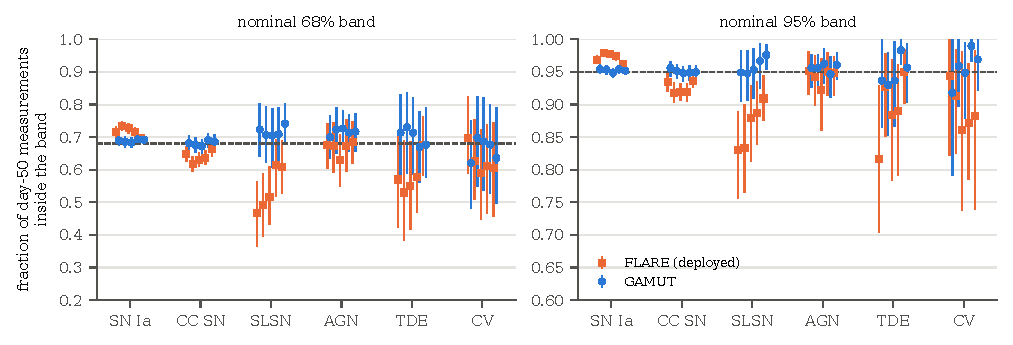
\includegraphics[width=\textwidth]{figures/day50.pdf}
\caption{Day-50 ZTF-BTS coverage slice following the diagnostic format of \citet{sasli2026forecast}: fraction of future measurements within 45--55 days post-detection falling inside the nominal 68\% (left) and 95\% (right) forecast bands per true spectroscopic class. Within each class, the five points from left to right correspond to forecast origins 5, 10, 15, 20, and 30 days, with vertical bars indicating 95\% object-level bootstrap intervals and dashed lines marking nominal levels.}
\label{fig:day50}
\end{figure}
\begin{table}[H]
\centering
\caption{Percentage of valid settings (six main benchmarks, all origins) under the bootstrap rule used in the main text and under the pre-registered fixed tolerance (worst class $\ge$ nominal $-0.02$ / $-0.015$).}
\label{tab:validity}
\scriptsize
\begin{tabular}{lcccc}
\toprule
 & \multicolumn{2}{c}{68\%} & \multicolumn{2}{c}{95\%} \\
\cmidrule(lr){2-3}\cmidrule(lr){4-5}
Method & bootstrap & tolerance & bootstrap & tolerance \\
\midrule
FLARE & 5 & 15 & 10 & 30 \\
Split CP & 5 & 5 & 5 & 10 \\
CQR & 5 & 10 & 0 & 10 \\
DCP & 0 & 10 & 0 & 15 \\
Localized CP & 10 & 15 & 5 & 10 \\
Label-shift mixture & 30 & 20 & 30 & 30 \\
GCC ($p$) & 20 & 20 & 15 & 30 \\
Learned partition & 30 & 20 & 25 & 30 \\
CPTC & 35 & 30 & 80 & 45 \\
Two-step CP & 100 & 100 & 100 & 100 \\
Kandinsky CP & 70 & 30 & 55 & 40 \\
MDCP & 100 & 100 & 100 & 80 \\
Max-class CP & 100 & 100 & 100 & 100 \\
Two-step CP + C1 & 100 & 100 & 100 & 100 \\
MDCP + C1 & 100 & 85 & 100 & 80 \\
Max-class CP + C1 & 100 & 100 & 100 & 100 \\
\gamut{} (ours) & 100 & 85 & 90 & 90 \\
\gamut-cert & 100 & 100 & 100 & 100 \\
True-class Mondrian (reference) & 85 & 75 & 90 & 75 \\
\bottomrule
\end{tabular}
\end{table}

\begin{table*}[t]
\centering
\caption{Per benchmark: worst-class coverage (minimum over origins) / mean band length relative to FLARE.}
\label{tab:perbench}
\scriptsize
\resizebox{\textwidth}{!}{%
\begin{tabular}{lcccccccc}
\toprule
Method & ZTF-BTS & PLAsTiCC-train & PLAsTiCC-DDF & StarLight & ECG5000 & ElecDevices & Wafer & PLAsTiCC-WFD (held out) \\
\midrule
\multicolumn{9}{l}{\textit{68\% bands}} \\
\midrule
FLARE & 0.514 / 1.00 & 0.385 / 1.00 & 0.371 / 1.00 & 0.675 / 1.00 & 0.613 / 1.00 & 0.616 / 1.00 & 0.679 / 1.00 & 0.266 / 1.00 \\
Split CP & 0.518 / 0.98 & 0.364 / 0.98 & 0.340 / 0.98 & 0.655 / 1.00 & 0.611 / 1.02 & 0.437 / 0.72 & 0.460 / 0.90 & 0.257 / 1.00 \\
CQR & 0.451 / 0.96 & 0.325 / 0.97 & 0.307 / 0.93 & 0.653 / 0.98 & 0.554 / 0.95 & 0.592 / 1.33 & 0.616 / 1.33 & 0.262 / 1.02 \\
DCP & 0.492 / 1.04 & 0.325 / 1.02 & 0.309 / 0.98 & 0.657 / 1.03 & 0.583 / 1.04 & 0.581 / 1.33 & 0.679 / 1.40 & 0.259 / 1.05 \\
Localized CP & 0.523 / 1.00 & 0.351 / 0.99 & 0.360 / 0.99 & 0.663 / 1.01 & 0.613 / 1.00 & 0.510 / 0.78 & 0.662 / 1.14 & 0.257 / 1.00 \\
Label-shift mixture & 0.541 / 1.01 & 0.403 / 1.02 & 0.398 / 1.01 & 0.677 / 1.01 & 0.616 / 1.01 & 0.650 / 0.97 & 0.680 / 1.01 & 0.349 / 1.05 \\
GCC ($p$) & 0.497 / 1.00 & 0.355 / 0.98 & 0.385 / 1.00 & 0.675 / 1.01 & 0.635 / 1.01 & 0.632 / 0.99 & 0.681 / 1.01 & 0.269 / 1.00 \\
Learned partition & 0.526 / 1.01 & 0.346 / 1.00 & 0.394 / 1.01 & 0.677 / 1.01 & 0.623 / 1.00 & 0.624 / 1.02 & 0.680 / 1.05 & 0.254 / 1.00 \\
CPTC & 0.514 / 0.97 & 0.522 / 1.10 & 0.334 / 0.96 & 0.676 / 1.00 & 0.594 / 1.00 & 0.666 / 1.04 & 0.678 / 0.89 & 0.333 / 1.14 \\
Two-step CP & 0.684 / 1.48 & 0.675 / 2.15 & 0.693 / 1.91 & 0.679 / 1.01 & 0.701 / 1.24 & 0.679 / 1.12 & 0.679 / 1.00 & 0.689 / 1.84 \\
Kandinsky CP & 0.623 / 1.03 & 0.461 / 1.26 & 0.548 / 1.10 & 0.676 / 1.00 & 0.645 / 1.05 & 0.656 / 1.00 & 0.676 / 1.00 & 0.563 / 2.33 \\
MDCP & 0.690 / 1.66 & 0.675 / 2.01 & 0.741 / 1.77 & 0.680 / 1.08 & 0.674 / 1.34 & 0.705 / 1.82 & 0.676 / 1.65 & 0.660 / 2.02 \\
Max-class CP & 0.695 / 1.58 & 0.675 / 2.15 & 0.699 / 1.93 & 0.680 / 1.06 & 0.701 / 1.25 & 0.680 / 1.31 & 0.680 / 1.73 & 0.698 / 1.84 \\
Two-step CP + C1 & 0.730 / 1.90 & 0.737 / 2.14 & 0.773 / 2.15 & 0.678 / 1.03 & 0.715 / 1.61 & 0.680 / 1.24 & 0.677 / 0.89 & 0.810 / 2.35 \\
MDCP + C1 & 0.678 / 1.85 & 0.652 / 2.06 & 0.697 / 1.83 & 0.681 / 1.12 & 0.658 / 1.62 & 0.691 / 1.80 & 0.673 / 1.89 & 0.673 / 2.00 \\
Max-class CP + C1 & 0.751 / 2.22 & 0.737 / 2.18 & 0.809 / 2.66 & 0.699 / 1.32 & 0.726 / 1.71 & 0.682 / 1.50 & 0.713 / 1.83 & 0.816 / 2.60 \\
\gamut{} (ours) & 0.659 / 1.02 & 0.651 / 1.33 & 0.669 / 1.21 & 0.680 / 1.00 & 0.668 / 1.06 & 0.680 / 1.00 & 0.683 / 0.91 & 0.665 / 1.51 \\
True-class Mondrian (reference) & 0.667 / 1.02 & 0.437 / 1.01 & 0.496 / 1.01 & 0.680 / 1.00 & 0.680 / 1.00 & 0.676 / 0.97 & 0.680 / 1.00 & 0.584 / 1.03 \\
\midrule
\multicolumn{9}{l}{\textit{95\% bands}} \\
\midrule
FLARE & 0.844 / 1.00 & 0.754 / 1.00 & 0.809 / 1.00 & 0.948 / 1.00 & 0.880 / 1.00 & 0.936 / 1.00 & 0.949 / 1.00 & 0.794 / 1.00 \\
Split CP & 0.847 / 0.98 & 0.747 / 0.93 & 0.774 / 0.96 & 0.929 / 0.98 & 0.878 / 1.02 & 0.909 / 0.80 & 0.873 / 0.96 & 0.790 / 1.00 \\
CQR & 0.799 / 0.98 & 0.723 / 0.87 & 0.769 / 0.91 & 0.933 / 0.97 & 0.837 / 1.02 & 0.910 / 0.78 & 0.898 / 1.22 & 0.684 / 0.95 \\
DCP & 0.836 / 1.18 & 0.753 / 1.02 & 0.845 / 1.14 & 0.946 / 1.16 & 0.868 / 1.33 & 0.914 / 0.80 & 0.936 / 1.58 & 0.704 / 1.01 \\
Localized CP & 0.849 / 0.99 & 0.754 / 0.94 & 0.808 / 0.98 & 0.934 / 0.99 & 0.872 / 1.00 & 0.915 / 0.84 & 0.768 / 0.90 & 0.783 / 0.99 \\
Label-shift mixture & 0.846 / 1.01 & 0.805 / 1.02 & 0.789 / 1.00 & 0.949 / 1.01 & 0.889 / 1.01 & 0.938 / 0.98 & 0.950 / 1.01 & 0.826 / 1.06 \\
GCC ($p$) & 0.835 / 1.00 & 0.744 / 0.92 & 0.792 / 0.98 & 0.946 / 1.00 & 0.885 / 1.02 & 0.938 / 0.96 & 0.951 / 1.01 & 0.777 / 0.98 \\
Learned partition & 0.844 / 1.01 & 0.747 / 0.97 & 0.809 / 0.99 & 0.949 / 1.01 & 0.898 / 1.01 & 0.938 / 1.00 & 0.950 / 1.04 & 0.785 / 1.00 \\
CPTC & 0.877 / 1.10 & 0.922 / 1.51 & 0.831 / 1.05 & 0.950 / 1.00 & 0.915 / 1.06 & 0.955 / 1.36 & 0.950 / 0.96 & 0.880 / 1.33 \\
Two-step CP & 0.950 / 1.63 & 0.941 / 2.25 & 0.962 / 2.08 & 0.949 / 1.00 & 0.936 / 2.01 & 0.958 / 2.19 & 0.949 / 1.00 & 0.967 / 1.95 \\
Kandinsky CP & 0.902 / 1.06 & 0.840 / 1.33 & 0.866 / 1.16 & 0.947 / 1.00 & 0.908 / 1.15 & 0.941 / 0.92 & 0.948 / 1.00 & 0.917 / 2.18 \\
MDCP & 0.950 / 1.80 & 0.926 / 1.46 & 0.952 / 1.54 & 0.949 / 1.04 & 0.911 / 1.59 & 0.950 / 1.32 & 0.949 / 1.46 & 0.936 / 1.49 \\
Max-class CP & 0.955 / 1.68 & 0.941 / 2.26 & 0.964 / 2.18 & 0.950 / 1.09 & 0.936 / 2.02 & 0.963 / 7.03 & 0.950 / 1.48 & 0.967 / 1.96 \\
Two-step CP + C1 & 0.958 / 1.78 & 0.960 / 2.14 & 0.973 / 1.94 & 0.949 / 1.01 & 0.943 / 2.15 & 0.959 / 1.46 & 0.948 / 0.95 & 0.984 / 1.96 \\
MDCP + C1 & 0.954 / 1.71 & 0.935 / 1.50 & 0.957 / 1.49 & 0.949 / 1.09 & 0.911 / 1.53 & 0.950 / 1.79 & 0.947 / 1.46 & 0.948 / 1.52 \\
Max-class CP + C1 & 0.966 / 2.00 & 0.960 / 2.17 & 0.981 / 2.43 & 0.957 / 1.27 & 0.944 / 2.16 & 0.962 / 3.46 & 0.958 / 1.79 & 0.984 / 2.13 \\
\gamut{} (ours) & 0.942 / 1.11 & 0.926 / 1.63 & 0.940 / 1.34 & 0.950 / 1.00 & 0.963 / 2.36 & 0.950 / 0.88 & 0.950 / 0.96 & 0.942 / 1.67 \\
True-class Mondrian (reference) & 0.937 / 1.01 & 0.792 / 0.99 & 0.925 / 1.01 & 0.950 / 1.00 & 0.936 / 1.01 & 0.949 / 1.13 & 0.950 / 1.00 & 0.920 / 0.99 \\
\bottomrule
\end{tabular}}
\end{table*}

\begin{table}[H]
\centering
\caption{ZTF-BTS, origin 5d, 68\% bands. Per-class coverage (point-pooled), worst class, CCG, mean length, interval score (IS) and class-averaged IS.}
\scriptsize
\resizebox{\textwidth}{!}{%
\begin{tabular}{lcccccccccccc}
\toprule
Method & Marg. & SN Ia & SN CC & SLSN & AGN & TDE & CV & Worst & CCG & Width & IS & cls-IS \\
\midrule
FLARE & 0.680 & 0.69 & 0.67 & 0.53 & 0.66 & 0.59 & 0.65 & 0.530 & 0.053 & 1.070 & 1.775 & 2.358 \\
Split CP & 0.680 & 0.69 & 0.67 & 0.55 & 0.66 & 0.58 & 0.62 & 0.548 & 0.057 & 1.075 & 1.775 & 2.344 \\
CQR & 0.680 & 0.69 & 0.68 & 0.54 & 0.65 & 0.59 & 0.61 & 0.535 & 0.057 & 1.056 & 1.764 & 2.314 \\
DCP & 0.680 & 0.67 & 0.71 & 0.54 & 0.66 & 0.59 & 0.64 & 0.543 & 0.053 & 1.087 & 1.771 & 2.304 \\
Localized CP & 0.680 & 0.69 & 0.67 & 0.54 & 0.66 & 0.58 & 0.62 & 0.540 & 0.057 & 1.070 & 1.774 & 2.346 \\
Label-shift mixture & 0.680 & 0.69 & 0.67 & 0.55 & 0.68 & 0.60 & 0.67 & 0.551 & 0.040 & 1.073 & 1.775 & 2.363 \\
GCC ($p$) & 0.682 & 0.69 & 0.67 & 0.54 & 0.63 & 0.57 & 0.63 & 0.537 & 0.061 & 1.074 & 1.776 & 2.361 \\
Learned partition & 0.680 & 0.69 & 0.67 & 0.54 & 0.65 & 0.59 & 0.65 & 0.540 & 0.054 & 1.072 & 1.775 & 2.355 \\
CPTC & 0.680 & 0.69 & 0.67 & 0.51 & 0.69 & 0.56 & 0.67 & 0.514 & 0.056 & 1.090 & 1.842 & 2.516 \\
Two-step CP & 0.815 & 0.83 & 0.81 & 0.69 & 0.77 & 0.73 & 0.73 & 0.689 & 0.080 & 1.530 & 1.924 & 2.432 \\
Kandinsky CP & 0.674 & 0.67 & 0.67 & 0.65 & 0.70 & 0.66 & 0.66 & 0.653 & 0.017 & 1.074 & 1.780 & 2.370 \\
MDCP & 0.747 & 0.73 & 0.78 & 0.73 & 0.76 & 0.80 & 0.70 & 0.697 & 0.070 & 1.582 & 2.151 & 2.489 \\
Max-class CP & 0.823 & 0.83 & 0.82 & 0.70 & 0.80 & 0.74 & 0.73 & 0.695 & 0.091 & 1.578 & 1.953 & 2.457 \\
Two-step CP + C1 & 0.844 & 0.84 & 0.87 & 0.80 & 0.78 & 0.87 & 0.77 & 0.767 & 0.141 & 1.769 & 2.078 & 2.390 \\
MDCP + C1 & 0.801 & 0.78 & 0.85 & 0.82 & 0.84 & 0.87 & 0.68 & 0.678 & 0.126 & 2.034 & 2.465 & 2.790 \\
Max-class CP + C1 & 0.889 & 0.89 & 0.91 & 0.81 & 0.86 & 0.88 & 0.78 & 0.782 & 0.175 & 2.114 & 2.359 & 2.589 \\
\gamut{} (ours) & 0.684 & 0.69 & 0.68 & 0.71 & 0.68 & 0.68 & 0.70 & 0.677 & 0.010 & 1.121 & 1.838 & 2.464 \\
True-class Mondrian (reference) & 0.680 & 0.68 & 0.68 & 0.67 & 0.68 & 0.67 & 0.69 & 0.673 & 0.004 & 1.076 & 1.770 & 2.357 \\
\gamut-cert (split certificate) & 0.804 & 0.81 & 0.80 & 0.78 & 0.79 & 0.76 & 0.80 & 0.762 & 0.110 & 1.536 & 1.962 & 2.610 \\
\gamut{} (point-level unit) & 0.681 & 0.68 & 0.68 & 0.68 & 0.69 & 0.69 & 0.68 & 0.680 & 0.004 & 1.107 & 1.832 & 2.466 \\
Union of class bands (early design) & 0.788 & 0.79 & 0.79 & 0.77 & 0.76 & 0.76 & 0.75 & 0.747 & 0.090 & 1.492 & 1.962 & 2.426 \\
\bottomrule
\end{tabular}}
\end{table}

\begin{table}[H]
\centering
\caption{ZTF-BTS, origin 10d, 68\% bands. Per-class coverage (point-pooled), worst class, CCG, mean length, interval score (IS) and class-averaged IS.}
\scriptsize
\resizebox{\textwidth}{!}{%
\begin{tabular}{lcccccccccccc}
\toprule
Method & Marg. & SN Ia & SN CC & SLSN & AGN & TDE & CV & Worst & CCG & Width & IS & cls-IS \\
\midrule
FLARE & 0.680 & 0.71 & 0.63 & 0.51 & 0.69 & 0.54 & 0.64 & 0.514 & 0.074 & 0.866 & 1.452 & 2.278 \\
Split CP & 0.680 & 0.72 & 0.62 & 0.52 & 0.62 & 0.56 & 0.63 & 0.518 & 0.082 & 0.863 & 1.453 & 2.267 \\
CQR & 0.680 & 0.73 & 0.61 & 0.48 & 0.61 & 0.52 & 0.60 & 0.483 & 0.104 & 0.847 & 1.453 & 2.248 \\
DCP & 0.680 & 0.71 & 0.63 & 0.49 & 0.63 & 0.54 & 0.66 & 0.492 & 0.079 & 0.895 & 1.460 & 2.233 \\
Localized CP & 0.681 & 0.71 & 0.63 & 0.52 & 0.66 & 0.56 & 0.63 & 0.523 & 0.072 & 0.870 & 1.449 & 2.265 \\
Label-shift mixture & 0.680 & 0.70 & 0.65 & 0.54 & 0.68 & 0.59 & 0.67 & 0.541 & 0.050 & 0.873 & 1.452 & 2.283 \\
GCC ($p$) & 0.680 & 0.71 & 0.63 & 0.50 & 0.69 & 0.58 & 0.64 & 0.497 & 0.069 & 0.867 & 1.452 & 2.278 \\
Learned partition & 0.680 & 0.71 & 0.64 & 0.53 & 0.70 & 0.56 & 0.65 & 0.526 & 0.066 & 0.873 & 1.449 & 2.271 \\
CPTC & 0.669 & 0.69 & 0.64 & 0.53 & 0.69 & 0.60 & 0.66 & 0.532 & 0.050 & 0.840 & 1.499 & 2.405 \\
Two-step CP & 0.844 & 0.87 & 0.80 & 0.68 & 0.78 & 0.75 & 0.77 & 0.684 & 0.096 & 1.373 & 1.650 & 2.375 \\
Kandinsky CP & 0.679 & 0.68 & 0.67 & 0.66 & 0.70 & 0.66 & 0.68 & 0.656 & 0.012 & 0.898 & 1.456 & 2.277 \\
MDCP & 0.878 & 0.89 & 0.87 & 0.76 & 0.85 & 0.84 & 0.71 & 0.710 & 0.140 & 1.597 & 1.840 & 2.420 \\
Max-class CP & 0.853 & 0.88 & 0.82 & 0.70 & 0.81 & 0.76 & 0.78 & 0.701 & 0.110 & 1.425 & 1.686 & 2.417 \\
Two-step CP + C1 & 0.863 & 0.86 & 0.88 & 0.81 & 0.76 & 0.83 & 0.76 & 0.760 & 0.138 & 1.665 & 1.868 & 2.286 \\
MDCP + C1 & 0.883 & 0.89 & 0.88 & 0.84 & 0.90 & 0.90 & 0.72 & 0.724 & 0.175 & 1.958 & 2.220 & 2.772 \\
Max-class CP + C1 & 0.925 & 0.94 & 0.92 & 0.83 & 0.86 & 0.87 & 0.77 & 0.770 & 0.185 & 1.970 & 2.104 & 2.490 \\
\gamut{} (ours) & 0.682 & 0.68 & 0.67 & 0.69 & 0.70 & 0.70 & 0.71 & 0.673 & 0.015 & 0.909 & 1.535 & 2.413 \\
True-class Mondrian (reference) & 0.680 & 0.68 & 0.68 & 0.67 & 0.68 & 0.68 & 0.68 & 0.669 & 0.003 & 0.884 & 1.439 & 2.259 \\
\gamut-cert (split certificate) & 0.796 & 0.80 & 0.79 & 0.74 & 0.82 & 0.80 & 0.82 & 0.742 & 0.117 & 1.233 & 1.615 & 2.525 \\
\gamut{} (point-level unit) & 0.681 & 0.68 & 0.68 & 0.69 & 0.69 & 0.69 & 0.69 & 0.679 & 0.007 & 0.910 & 1.534 & 2.411 \\
Union of class bands (early design) & 0.800 & 0.80 & 0.80 & 0.77 & 0.78 & 0.81 & 0.75 & 0.753 & 0.107 & 1.270 & 1.635 & 2.292 \\
\bottomrule
\end{tabular}}
\end{table}

\begin{table}[H]
\centering
\caption{ZTF-BTS, origin 15d, 68\% bands. Per-class coverage (point-pooled), worst class, CCG, mean length, interval score (IS) and class-averaged IS.}
\scriptsize
\resizebox{\textwidth}{!}{%
\begin{tabular}{lcccccccccccc}
\toprule
Method & Marg. & SN Ia & SN CC & SLSN & AGN & TDE & CV & Worst & CCG & Width & IS & cls-IS \\
\midrule
FLARE & 0.680 & 0.72 & 0.63 & 0.53 & 0.65 & 0.57 & 0.62 & 0.534 & 0.071 & 0.782 & 1.305 & 2.226 \\
Split CP & 0.680 & 0.73 & 0.61 & 0.53 & 0.59 & 0.56 & 0.57 & 0.534 & 0.099 & 0.774 & 1.307 & 2.239 \\
CQR & 0.680 & 0.74 & 0.59 & 0.49 & 0.57 & 0.53 & 0.54 & 0.493 & 0.123 & 0.743 & 1.310 & 2.209 \\
DCP & 0.680 & 0.73 & 0.61 & 0.50 & 0.61 & 0.55 & 0.61 & 0.503 & 0.093 & 0.813 & 1.327 & 2.188 \\
Localized CP & 0.680 & 0.72 & 0.63 & 0.55 & 0.64 & 0.57 & 0.58 & 0.549 & 0.078 & 0.784 & 1.303 & 2.218 \\
Label-shift mixture & 0.680 & 0.70 & 0.65 & 0.58 & 0.68 & 0.61 & 0.65 & 0.582 & 0.042 & 0.793 & 1.307 & 2.230 \\
GCC ($p$) & 0.677 & 0.71 & 0.63 & 0.55 & 0.66 & 0.59 & 0.60 & 0.545 & 0.067 & 0.781 & 1.306 & 2.247 \\
Learned partition & 0.680 & 0.71 & 0.63 & 0.55 & 0.65 & 0.59 & 0.62 & 0.554 & 0.064 & 0.792 & 1.303 & 2.216 \\
CPTC & 0.663 & 0.68 & 0.63 & 0.59 & 0.69 & 0.67 & 0.65 & 0.590 & 0.033 & 0.736 & 1.351 & 2.267 \\
Two-step CP & 0.842 & 0.88 & 0.79 & 0.73 & 0.77 & 0.76 & 0.76 & 0.728 & 0.101 & 1.203 & 1.462 & 2.336 \\
Kandinsky CP & 0.678 & 0.69 & 0.67 & 0.66 & 0.68 & 0.65 & 0.62 & 0.623 & 0.021 & 0.814 & 1.310 & 2.262 \\
MDCP & 0.780 & 0.79 & 0.77 & 0.69 & 0.77 & 0.74 & 0.72 & 0.690 & 0.066 & 1.192 & 1.582 & 2.291 \\
Max-class CP & 0.861 & 0.89 & 0.82 & 0.75 & 0.82 & 0.76 & 0.76 & 0.746 & 0.120 & 1.316 & 1.536 & 2.398 \\
Two-step CP + C1 & 0.855 & 0.85 & 0.87 & 0.80 & 0.79 & 0.84 & 0.75 & 0.748 & 0.137 & 1.554 & 1.743 & 2.237 \\
MDCP + C1 & 0.761 & 0.76 & 0.76 & 0.72 & 0.77 & 0.78 & 0.72 & 0.719 & 0.073 & 1.197 & 1.669 & 2.460 \\
Max-class CP + C1 & 0.910 & 0.92 & 0.91 & 0.83 & 0.87 & 0.86 & 0.76 & 0.757 & 0.177 & 1.767 & 1.906 & 2.414 \\
\gamut{} (ours) & 0.679 & 0.68 & 0.67 & 0.69 & 0.70 & 0.66 & 0.68 & 0.664 & 0.009 & 0.783 & 1.373 & 2.310 \\
True-class Mondrian (reference) & 0.680 & 0.68 & 0.68 & 0.68 & 0.67 & 0.68 & 0.68 & 0.674 & 0.002 & 0.804 & 1.293 & 2.207 \\
\gamut-cert (split certificate) & 0.767 & 0.77 & 0.76 & 0.79 & 0.82 & 0.78 & 0.77 & 0.764 & 0.102 & 1.052 & 1.447 & 2.438 \\
\gamut{} (point-level unit) & 0.681 & 0.68 & 0.68 & 0.68 & 0.68 & 0.69 & 0.68 & 0.680 & 0.003 & 0.788 & 1.372 & 2.307 \\
Union of class bands (early design) & 0.725 & 0.73 & 0.71 & 0.74 & 0.73 & 0.77 & 0.72 & 0.713 & 0.053 & 0.903 & 1.367 & 2.090 \\
\bottomrule
\end{tabular}}
\end{table}

\begin{table}[H]
\centering
\caption{ZTF-BTS, origin 20d, 68\% bands. Per-class coverage (point-pooled), worst class, CCG, mean length, interval score (IS) and class-averaged IS.}
\scriptsize
\resizebox{\textwidth}{!}{%
\begin{tabular}{lcccccccccccc}
\toprule
Method & Marg. & SN Ia & SN CC & SLSN & AGN & TDE & CV & Worst & CCG & Width & IS & cls-IS \\
\midrule
FLARE & 0.680 & 0.71 & 0.63 & 0.61 & 0.69 & 0.60 & 0.64 & 0.603 & 0.046 & 0.678 & 1.141 & 2.031 \\
Split CP & 0.680 & 0.73 & 0.61 & 0.58 & 0.64 & 0.60 & 0.55 & 0.551 & 0.079 & 0.662 & 1.143 & 2.041 \\
CQR & 0.680 & 0.75 & 0.58 & 0.53 & 0.57 & 0.54 & 0.51 & 0.508 & 0.125 & 0.643 & 1.161 & 2.085 \\
DCP & 0.680 & 0.74 & 0.60 & 0.53 & 0.60 & 0.58 & 0.59 & 0.534 & 0.093 & 0.722 & 1.186 & 2.071 \\
Localized CP & 0.679 & 0.71 & 0.63 & 0.60 & 0.68 & 0.62 & 0.58 & 0.581 & 0.054 & 0.676 & 1.140 & 2.029 \\
Label-shift mixture & 0.680 & 0.70 & 0.65 & 0.63 & 0.68 & 0.64 & 0.64 & 0.630 & 0.029 & 0.687 & 1.142 & 2.023 \\
GCC ($p$) & 0.681 & 0.71 & 0.64 & 0.62 & 0.69 & 0.63 & 0.60 & 0.599 & 0.046 & 0.682 & 1.143 & 2.046 \\
Learned partition & 0.680 & 0.71 & 0.64 & 0.62 & 0.69 & 0.63 & 0.63 & 0.620 & 0.040 & 0.688 & 1.139 & 2.023 \\
CPTC & 0.671 & 0.69 & 0.65 & 0.63 & 0.70 & 0.67 & 0.66 & 0.633 & 0.022 & 0.644 & 1.136 & 2.000 \\
Two-step CP & 0.805 & 0.84 & 0.75 & 0.73 & 0.77 & 0.77 & 0.72 & 0.722 & 0.082 & 0.947 & 1.233 & 2.118 \\
Kandinsky CP & 0.684 & 0.68 & 0.69 & 0.68 & 0.69 & 0.67 & 0.63 & 0.631 & 0.015 & 0.712 & 1.144 & 2.035 \\
MDCP & 0.848 & 0.87 & 0.82 & 0.74 & 0.83 & 0.80 & 0.72 & 0.715 & 0.115 & 1.229 & 1.480 & 2.267 \\
Max-class CP & 0.840 & 0.87 & 0.80 & 0.75 & 0.82 & 0.78 & 0.73 & 0.728 & 0.113 & 1.086 & 1.315 & 2.185 \\
Two-step CP + C1 & 0.842 & 0.85 & 0.84 & 0.79 & 0.76 & 0.83 & 0.73 & 0.730 & 0.122 & 1.302 & 1.498 & 2.093 \\
MDCP + C1 & 0.844 & 0.87 & 0.80 & 0.74 & 0.88 & 0.83 & 0.77 & 0.742 & 0.136 & 1.196 & 1.517 & 2.437 \\
Max-class CP + C1 & 0.895 & 0.90 & 0.90 & 0.82 & 0.87 & 0.86 & 0.75 & 0.751 & 0.170 & 1.553 & 1.697 & 2.309 \\
\gamut{} (ours) & 0.689 & 0.69 & 0.69 & 0.71 & 0.70 & 0.68 & 0.67 & 0.669 & 0.013 & 0.677 & 1.161 & 2.054 \\
True-class Mondrian (reference) & 0.680 & 0.68 & 0.68 & 0.68 & 0.68 & 0.67 & 0.68 & 0.670 & 0.003 & 0.695 & 1.133 & 2.011 \\
\gamut-cert (split certificate) & 0.813 & 0.82 & 0.80 & 0.79 & 0.85 & 0.80 & 0.84 & 0.787 & 0.138 & 0.962 & 1.244 & 2.264 \\
\gamut{} (point-level unit) & 0.681 & 0.68 & 0.68 & 0.69 & 0.69 & 0.69 & 0.68 & 0.681 & 0.004 & 0.663 & 1.163 & 2.077 \\
Union of class bands (early design) & 0.791 & 0.81 & 0.77 & 0.76 & 0.82 & 0.78 & 0.76 & 0.759 & 0.102 & 0.902 & 1.229 & 2.099 \\
\bottomrule
\end{tabular}}
\end{table}

\begin{table}[H]
\centering
\caption{ZTF-BTS, origin 30d, 68\% bands. Per-class coverage (point-pooled), worst class, CCG, mean length, interval score (IS) and class-averaged IS.}
\scriptsize
\resizebox{\textwidth}{!}{%
\begin{tabular}{lcccccccccccc}
\toprule
Method & Marg. & SN Ia & SN CC & SLSN & AGN & TDE & CV & Worst & CCG & Width & IS & cls-IS \\
\midrule
FLARE & 0.680 & 0.69 & 0.67 & 0.61 & 0.68 & 0.66 & 0.64 & 0.615 & 0.026 & 0.580 & 0.954 & 1.810 \\
Split CP & 0.680 & 0.74 & 0.61 & 0.55 & 0.61 & 0.58 & 0.59 & 0.553 & 0.087 & 0.552 & 0.956 & 1.789 \\
CQR & 0.680 & 0.75 & 0.60 & 0.56 & 0.55 & 0.56 & 0.45 & 0.451 & 0.125 & 0.530 & 0.967 & 1.834 \\
DCP & 0.680 & 0.73 & 0.62 & 0.61 & 0.61 & 0.63 & 0.54 & 0.537 & 0.074 & 0.602 & 0.995 & 1.812 \\
Localized CP & 0.677 & 0.70 & 0.66 & 0.59 & 0.66 & 0.62 & 0.62 & 0.587 & 0.045 & 0.571 & 0.950 & 1.782 \\
Label-shift mixture & 0.682 & 0.69 & 0.67 & 0.63 & 0.67 & 0.66 & 0.66 & 0.632 & 0.019 & 0.584 & 0.951 & 1.790 \\
GCC ($p$) & 0.677 & 0.69 & 0.67 & 0.64 & 0.67 & 0.66 & 0.64 & 0.635 & 0.023 & 0.575 & 0.952 & 1.797 \\
Learned partition & 0.680 & 0.69 & 0.67 & 0.63 & 0.68 & 0.67 & 0.66 & 0.626 & 0.018 & 0.587 & 0.951 & 1.790 \\
CPTC & 0.682 & 0.69 & 0.67 & 0.64 & 0.68 & 0.70 & 0.67 & 0.639 & 0.016 & 0.569 & 0.938 & 1.797 \\
Two-step CP & 0.798 & 0.82 & 0.78 & 0.71 & 0.76 & 0.80 & 0.72 & 0.715 & 0.085 & 0.841 & 1.066 & 1.888 \\
Kandinsky CP & 0.678 & 0.68 & 0.68 & 0.63 & 0.68 & 0.65 & 0.68 & 0.627 & 0.016 & 0.582 & 0.952 & 1.839 \\
MDCP & 0.836 & 0.89 & 0.78 & 0.73 & 0.77 & 0.83 & 0.76 & 0.729 & 0.112 & 0.947 & 1.205 & 1.995 \\
Max-class CP & 0.816 & 0.85 & 0.78 & 0.72 & 0.79 & 0.81 & 0.74 & 0.716 & 0.100 & 0.871 & 1.084 & 1.910 \\
Two-step CP + C1 & 0.881 & 0.91 & 0.86 & 0.77 & 0.76 & 0.86 & 0.75 & 0.752 & 0.140 & 1.177 & 1.330 & 1.960 \\
MDCP + C1 & 0.866 & 0.92 & 0.81 & 0.76 & 0.81 & 0.88 & 0.77 & 0.764 & 0.145 & 1.034 & 1.298 & 2.157 \\
Max-class CP + C1 & 0.907 & 0.93 & 0.89 & 0.83 & 0.83 & 0.89 & 0.79 & 0.790 & 0.180 & 1.339 & 1.467 & 2.167 \\
\gamut{} (ours) & 0.688 & 0.69 & 0.69 & 0.69 & 0.70 & 0.73 & 0.66 & 0.659 & 0.020 & 0.579 & 0.949 & 1.862 \\
True-class Mondrian (reference) & 0.680 & 0.68 & 0.68 & 0.68 & 0.68 & 0.68 & 0.67 & 0.667 & 0.003 & 0.585 & 0.952 & 1.793 \\
\gamut-cert (split certificate) & 0.768 & 0.77 & 0.77 & 0.75 & 0.79 & 0.83 & 0.78 & 0.751 & 0.101 & 0.745 & 1.007 & 2.003 \\
\gamut{} (point-level unit) & 0.682 & 0.68 & 0.68 & 0.69 & 0.68 & 0.69 & 0.68 & 0.680 & 0.004 & 0.569 & 0.949 & 1.874 \\
Union of class bands (early design) & 0.757 & 0.76 & 0.75 & 0.73 & 0.73 & 0.78 & 0.74 & 0.726 & 0.069 & 0.700 & 0.982 & 1.823 \\
\bottomrule
\end{tabular}}
\end{table}

\begin{table}[H]
\centering
\caption{ZTF-BTS, origin 5d, 95\% bands. Per-class coverage (point-pooled), worst class, CCG, mean length, interval score (IS) and class-averaged IS.}
\scriptsize
\resizebox{\textwidth}{!}{%
\begin{tabular}{lcccccccccccc}
\toprule
Method & Marg. & SN Ia & SN CC & SLSN & AGN & TDE & CV & Worst & CCG & Width & IS & cls-IS \\
\midrule
FLARE & 0.949 & 0.96 & 0.94 & 0.85 & 0.93 & 0.90 & 0.93 & 0.852 & 0.034 & 2.525 & 3.251 & 4.479 \\
Split CP & 0.950 & 0.96 & 0.95 & 0.86 & 0.91 & 0.91 & 0.90 & 0.862 & 0.037 & 2.549 & 3.258 & 4.370 \\
CQR & 0.950 & 0.95 & 0.96 & 0.88 & 0.93 & 0.93 & 0.86 & 0.863 & 0.034 & 2.465 & 3.215 & 4.300 \\
DCP & 0.950 & 0.95 & 0.96 & 0.90 & 0.94 & 0.95 & 0.87 & 0.874 & 0.027 & 2.674 & 3.346 & 4.244 \\
Localized CP & 0.949 & 0.96 & 0.94 & 0.85 & 0.92 & 0.90 & 0.91 & 0.855 & 0.037 & 2.505 & 3.245 & 4.407 \\
Label-shift mixture & 0.949 & 0.96 & 0.94 & 0.85 & 0.94 & 0.91 & 0.94 & 0.851 & 0.030 & 2.521 & 3.268 & 4.557 \\
GCC ($p$) & 0.950 & 0.96 & 0.94 & 0.86 & 0.93 & 0.89 & 0.92 & 0.855 & 0.036 & 2.532 & 3.266 & 4.537 \\
Learned partition & 0.949 & 0.96 & 0.94 & 0.86 & 0.93 & 0.91 & 0.93 & 0.856 & 0.032 & 2.535 & 3.264 & 4.438 \\
CPTC & 0.966 & 0.97 & 0.96 & 0.89 & 0.95 & 0.95 & 0.94 & 0.894 & 0.019 & 2.865 & 3.369 & 4.382 \\
Two-step CP & 0.984 & 0.99 & 0.98 & 0.96 & 0.97 & 0.98 & 0.96 & 0.961 & 0.024 & 3.790 & 3.996 & 4.721 \\
Kandinsky CP & 0.949 & 0.95 & 0.95 & 0.93 & 0.95 & 0.94 & 0.94 & 0.928 & 0.007 & 2.647 & 3.398 & 4.686 \\
MDCP & 0.987 & 0.99 & 0.99 & 0.95 & 0.97 & 0.99 & 0.96 & 0.950 & 0.025 & 3.910 & 4.126 & 4.404 \\
Max-class CP & 0.986 & 0.99 & 0.99 & 0.97 & 0.97 & 0.98 & 0.97 & 0.966 & 0.027 & 4.020 & 4.198 & 4.864 \\
Two-step CP + C1 & 0.989 & 0.99 & 0.99 & 0.97 & 0.98 & 1.00 & 0.96 & 0.958 & 0.031 & 3.944 & 4.087 & 4.542 \\
MDCP + C1 & 0.989 & 0.99 & 1.00 & 0.99 & 0.99 & 1.00 & 0.95 & 0.954 & 0.034 & 4.513 & 4.679 & 4.957 \\
Max-class CP + C1 & 0.994 & 0.99 & 1.00 & 0.97 & 0.99 & 1.00 & 0.97 & 0.968 & 0.036 & 4.536 & 4.631 & 4.867 \\
\gamut{} (ours) & 0.952 & 0.95 & 0.95 & 0.96 & 0.95 & 0.95 & 0.95 & 0.948 & 0.003 & 2.910 & 3.488 & 4.694 \\
True-class Mondrian (reference) & 0.950 & 0.95 & 0.95 & 0.95 & 0.94 & 0.95 & 0.95 & 0.939 & 0.004 & 2.489 & 3.192 & 4.323 \\
\gamut-cert (split certificate) & 0.989 & 0.99 & 0.99 & 0.99 & 0.99 & 0.97 & 0.98 & 0.971 & 0.036 & 4.671 & 4.798 & 5.769 \\
\gamut{} (point-level unit) & 0.950 & 0.95 & 0.95 & 0.96 & 0.96 & 0.96 & 0.95 & 0.949 & 0.004 & 2.889 & 3.499 & 4.735 \\
Union of class bands (early design) & 0.986 & 0.99 & 0.99 & 0.96 & 0.95 & 1.00 & 0.96 & 0.951 & 0.024 & 3.774 & 3.954 & 4.403 \\
\bottomrule
\end{tabular}}
\end{table}

\begin{table}[H]
\centering
\caption{ZTF-BTS, origin 10d, 95\% bands. Per-class coverage (point-pooled), worst class, CCG, mean length, interval score (IS) and class-averaged IS.}
\scriptsize
\resizebox{\textwidth}{!}{%
\begin{tabular}{lcccccccccccc}
\toprule
Method & Marg. & SN Ia & SN CC & SLSN & AGN & TDE & CV & Worst & CCG & Width & IS & cls-IS \\
\midrule
FLARE & 0.949 & 0.97 & 0.92 & 0.84 & 0.95 & 0.90 & 0.91 & 0.844 & 0.039 & 2.095 & 2.718 & 4.426 \\
Split CP & 0.950 & 0.97 & 0.93 & 0.85 & 0.91 & 0.89 & 0.90 & 0.847 & 0.048 & 2.099 & 2.717 & 4.367 \\
CQR & 0.950 & 0.97 & 0.94 & 0.83 & 0.90 & 0.87 & 0.86 & 0.825 & 0.062 & 2.074 & 2.687 & 4.370 \\
DCP & 0.950 & 0.96 & 0.95 & 0.86 & 0.91 & 0.89 & 0.89 & 0.855 & 0.044 & 2.306 & 2.837 & 4.271 \\
Localized CP & 0.950 & 0.97 & 0.93 & 0.85 & 0.93 & 0.90 & 0.91 & 0.849 & 0.043 & 2.107 & 2.714 & 4.303 \\
Label-shift mixture & 0.946 & 0.96 & 0.93 & 0.85 & 0.94 & 0.91 & 0.94 & 0.846 & 0.033 & 2.119 & 2.776 & 4.556 \\
GCC ($p$) & 0.948 & 0.97 & 0.92 & 0.84 & 0.95 & 0.90 & 0.92 & 0.835 & 0.041 & 2.093 & 2.727 & 4.420 \\
Learned partition & 0.949 & 0.97 & 0.92 & 0.84 & 0.95 & 0.89 & 0.92 & 0.844 & 0.040 & 2.109 & 2.731 & 4.388 \\
CPTC & 0.961 & 0.97 & 0.95 & 0.88 & 0.95 & 0.95 & 0.95 & 0.877 & 0.017 & 2.313 & 2.812 & 4.328 \\
Two-step CP & 0.989 & 0.99 & 0.98 & 0.96 & 0.98 & 0.97 & 0.97 & 0.957 & 0.027 & 3.641 & 3.752 & 4.932 \\
Kandinsky CP & 0.947 & 0.95 & 0.94 & 0.93 & 0.93 & 0.93 & 0.94 & 0.925 & 0.014 & 2.241 & 2.825 & 4.405 \\
MDCP & 0.995 & 1.00 & 0.99 & 0.96 & 0.99 & 0.99 & 0.96 & 0.956 & 0.031 & 3.818 & 3.897 & 4.422 \\
Max-class CP & 0.991 & 1.00 & 0.99 & 0.96 & 0.99 & 0.98 & 0.98 & 0.958 & 0.030 & 3.770 & 3.859 & 5.059 \\
Two-step CP + C1 & 0.991 & 0.99 & 0.99 & 0.97 & 0.98 & 0.98 & 0.97 & 0.965 & 0.031 & 3.685 & 3.778 & 4.316 \\
MDCP + C1 & 0.994 & 1.00 & 0.99 & 0.97 & 1.00 & 0.99 & 0.96 & 0.965 & 0.036 & 3.834 & 3.910 & 4.564 \\
Max-class CP + C1 & 0.997 & 1.00 & 1.00 & 0.97 & 1.00 & 0.99 & 0.97 & 0.966 & 0.037 & 4.252 & 4.305 & 4.704 \\
\gamut{} (ours) & 0.952 & 0.95 & 0.95 & 0.95 & 0.96 & 0.94 & 0.96 & 0.942 & 0.005 & 2.481 & 3.005 & 4.622 \\
True-class Mondrian (reference) & 0.950 & 0.95 & 0.95 & 0.95 & 0.94 & 0.94 & 0.95 & 0.943 & 0.002 & 2.099 & 2.616 & 4.307 \\
\gamut-cert (split certificate) & 0.990 & 0.99 & 0.99 & 1.00 & 0.99 & 0.99 & 0.99 & 0.987 & 0.042 & 4.298 & 4.380 & 5.502 \\
\gamut{} (point-level unit) & 0.952 & 0.95 & 0.95 & 0.95 & 0.95 & 0.94 & 0.96 & 0.943 & 0.005 & 2.545 & 3.079 & 4.720 \\
Union of class bands (early design) & 0.995 & 1.00 & 0.99 & 0.98 & 0.99 & 0.98 & 0.97 & 0.970 & 0.035 & 4.252 & 4.304 & 4.744 \\
\bottomrule
\end{tabular}}
\end{table}

\begin{table}[H]
\centering
\caption{ZTF-BTS, origin 15d, 95\% bands. Per-class coverage (point-pooled), worst class, CCG, mean length, interval score (IS) and class-averaged IS.}
\scriptsize
\resizebox{\textwidth}{!}{%
\begin{tabular}{lcccccccccccc}
\toprule
Method & Marg. & SN Ia & SN CC & SLSN & AGN & TDE & CV & Worst & CCG & Width & IS & cls-IS \\
\midrule
FLARE & 0.950 & 0.97 & 0.92 & 0.89 & 0.95 & 0.87 & 0.90 & 0.872 & 0.040 & 1.892 & 2.491 & 4.356 \\
Split CP & 0.950 & 0.97 & 0.93 & 0.89 & 0.93 & 0.87 & 0.88 & 0.868 & 0.046 & 1.865 & 2.469 & 4.237 \\
CQR & 0.950 & 0.97 & 0.93 & 0.83 & 0.90 & 0.84 & 0.82 & 0.825 & 0.074 & 1.872 & 2.479 & 4.502 \\
DCP & 0.950 & 0.96 & 0.94 & 0.85 & 0.92 & 0.87 & 0.86 & 0.849 & 0.054 & 2.218 & 2.696 & 4.318 \\
Localized CP & 0.950 & 0.97 & 0.92 & 0.89 & 0.93 & 0.87 & 0.90 & 0.875 & 0.042 & 1.884 & 2.474 & 4.225 \\
Label-shift mixture & 0.946 & 0.96 & 0.93 & 0.88 & 0.96 & 0.89 & 0.93 & 0.885 & 0.030 & 1.908 & 2.530 & 4.447 \\
GCC ($p$) & 0.948 & 0.97 & 0.92 & 0.88 & 0.94 & 0.88 & 0.91 & 0.877 & 0.040 & 1.877 & 2.484 & 4.371 \\
Learned partition & 0.949 & 0.97 & 0.92 & 0.89 & 0.94 & 0.88 & 0.91 & 0.877 & 0.039 & 1.890 & 2.487 & 4.272 \\
CPTC & 0.958 & 0.97 & 0.95 & 0.92 & 0.96 & 0.94 & 0.95 & 0.923 & 0.012 & 2.038 & 2.513 & 3.902 \\
Two-step CP & 0.989 & 0.99 & 0.98 & 0.97 & 0.99 & 0.95 & 0.97 & 0.955 & 0.025 & 3.291 & 3.440 & 5.024 \\
Kandinsky CP & 0.949 & 0.95 & 0.94 & 0.95 & 0.96 & 0.90 & 0.93 & 0.902 & 0.015 & 2.086 & 2.642 & 4.492 \\
MDCP & 0.995 & 1.00 & 0.99 & 0.97 & 0.99 & 0.97 & 0.96 & 0.964 & 0.031 & 3.687 & 3.758 & 4.646 \\
Max-class CP & 0.989 & 1.00 & 0.98 & 0.97 & 0.99 & 0.96 & 0.97 & 0.955 & 0.027 & 3.358 & 3.496 & 5.117 \\
Two-step CP + C1 & 0.993 & 0.99 & 0.99 & 0.97 & 0.98 & 0.97 & 0.97 & 0.967 & 0.031 & 3.566 & 3.638 & 4.442 \\
MDCP + C1 & 0.994 & 1.00 & 0.99 & 0.97 & 0.99 & 0.97 & 0.96 & 0.964 & 0.031 & 3.350 & 3.424 & 4.374 \\
Max-class CP + C1 & 0.997 & 1.00 & 1.00 & 0.98 & 0.99 & 0.98 & 0.97 & 0.973 & 0.035 & 3.975 & 4.025 & 4.758 \\
\gamut{} (ours) & 0.948 & 0.95 & 0.95 & 0.96 & 0.96 & 0.95 & 0.94 & 0.943 & 0.006 & 2.038 & 2.591 & 4.268 \\
True-class Mondrian (reference) & 0.950 & 0.95 & 0.95 & 0.95 & 0.95 & 0.94 & 0.95 & 0.940 & 0.003 & 1.922 & 2.433 & 4.578 \\
\gamut-cert (split certificate) & 0.987 & 0.99 & 0.99 & 0.99 & 0.99 & 1.00 & 0.98 & 0.983 & 0.038 & 3.545 & 3.687 & 5.364 \\
\gamut{} (point-level unit) & 0.951 & 0.95 & 0.95 & 0.95 & 0.96 & 0.95 & 0.95 & 0.949 & 0.003 & 2.053 & 2.569 & 4.302 \\
Union of class bands (early design) & 0.996 & 1.00 & 1.00 & 0.98 & 0.99 & 0.98 & 0.98 & 0.978 & 0.039 & 4.276 & 4.317 & 5.127 \\
\bottomrule
\end{tabular}}
\end{table}

\begin{table}[H]
\centering
\caption{ZTF-BTS, origin 20d, 95\% bands. Per-class coverage (point-pooled), worst class, CCG, mean length, interval score (IS) and class-averaged IS.}
\scriptsize
\resizebox{\textwidth}{!}{%
\begin{tabular}{lcccccccccccc}
\toprule
Method & Marg. & SN Ia & SN CC & SLSN & AGN & TDE & CV & Worst & CCG & Width & IS & cls-IS \\
\midrule
FLARE & 0.949 & 0.97 & 0.92 & 0.91 & 0.96 & 0.90 & 0.90 & 0.901 & 0.030 & 1.741 & 2.273 & 4.046 \\
Split CP & 0.950 & 0.97 & 0.92 & 0.90 & 0.93 & 0.91 & 0.90 & 0.896 & 0.035 & 1.679 & 2.251 & 3.821 \\
CQR & 0.950 & 0.97 & 0.93 & 0.81 & 0.90 & 0.88 & 0.80 & 0.799 & 0.075 & 1.705 & 2.269 & 4.420 \\
DCP & 0.950 & 0.96 & 0.94 & 0.84 & 0.92 & 0.89 & 0.84 & 0.836 & 0.056 & 2.128 & 2.556 & 4.275 \\
Localized CP & 0.950 & 0.97 & 0.92 & 0.91 & 0.95 & 0.92 & 0.92 & 0.912 & 0.025 & 1.719 & 2.252 & 3.828 \\
Label-shift mixture & 0.948 & 0.96 & 0.93 & 0.92 & 0.95 & 0.93 & 0.93 & 0.922 & 0.017 & 1.758 & 2.295 & 4.117 \\
GCC ($p$) & 0.950 & 0.97 & 0.92 & 0.92 & 0.96 & 0.91 & 0.92 & 0.908 & 0.026 & 1.735 & 2.269 & 3.873 \\
Learned partition & 0.949 & 0.96 & 0.93 & 0.92 & 0.96 & 0.91 & 0.92 & 0.912 & 0.025 & 1.757 & 2.273 & 3.938 \\
CPTC & 0.960 & 0.97 & 0.95 & 0.94 & 0.96 & 0.97 & 0.95 & 0.940 & 0.009 & 1.872 & 2.264 & 3.693 \\
Two-step CP & 0.986 & 0.99 & 0.98 & 0.97 & 0.98 & 0.96 & 0.98 & 0.963 & 0.027 & 2.826 & 2.987 & 4.746 \\
Kandinsky CP & 0.951 & 0.95 & 0.95 & 0.94 & 0.96 & 0.94 & 0.95 & 0.937 & 0.007 & 1.876 & 2.320 & 4.183 \\
MDCP & 0.995 & 1.00 & 0.99 & 0.97 & 0.99 & 0.99 & 0.99 & 0.967 & 0.038 & 3.409 & 3.479 & 4.587 \\
Max-class CP & 0.988 & 0.99 & 0.98 & 0.98 & 0.98 & 0.96 & 0.98 & 0.963 & 0.029 & 2.920 & 3.065 & 4.828 \\
Two-step CP + C1 & 0.989 & 0.99 & 0.99 & 0.96 & 0.98 & 0.99 & 0.98 & 0.961 & 0.032 & 3.165 & 3.254 & 4.263 \\
MDCP + C1 & 0.993 & 1.00 & 0.99 & 0.97 & 0.99 & 0.99 & 0.99 & 0.969 & 0.038 & 2.896 & 2.986 & 4.268 \\
Max-class CP + C1 & 0.994 & 1.00 & 0.99 & 0.97 & 1.00 & 0.99 & 0.98 & 0.971 & 0.038 & 3.503 & 3.562 & 4.587 \\
\gamut{} (ours) & 0.952 & 0.95 & 0.95 & 0.96 & 0.96 & 0.97 & 0.96 & 0.951 & 0.009 & 1.816 & 2.235 & 4.027 \\
True-class Mondrian (reference) & 0.950 & 0.95 & 0.95 & 0.95 & 0.95 & 0.94 & 0.94 & 0.944 & 0.003 & 1.780 & 2.240 & 4.241 \\
\gamut-cert (split certificate) & 0.992 & 0.99 & 0.99 & 0.99 & 0.99 & 1.00 & 1.00 & 0.985 & 0.043 & 3.066 & 3.143 & 5.144 \\
\gamut{} (point-level unit) & 0.951 & 0.95 & 0.95 & 0.96 & 0.95 & 0.97 & 0.96 & 0.951 & 0.007 & 1.813 & 2.231 & 3.910 \\
Union of class bands (early design) & 0.997 & 1.00 & 1.00 & 0.98 & 1.00 & 0.99 & 1.00 & 0.982 & 0.043 & 5.000 & 5.031 & 6.312 \\
\bottomrule
\end{tabular}}
\end{table}

\begin{table}[H]
\centering
\caption{ZTF-BTS, origin 30d, 95\% bands. Per-class coverage (point-pooled), worst class, CCG, mean length, interval score (IS) and class-averaged IS.}
\scriptsize
\resizebox{\textwidth}{!}{%
\begin{tabular}{lcccccccccccc}
\toprule
Method & Marg. & SN Ia & SN CC & SLSN & AGN & TDE & CV & Worst & CCG & Width & IS & cls-IS \\
\midrule
FLARE & 0.949 & 0.96 & 0.94 & 0.91 & 0.95 & 0.95 & 0.88 & 0.881 & 0.023 & 1.480 & 1.904 & 3.893 \\
Split CP & 0.950 & 0.97 & 0.92 & 0.87 & 0.93 & 0.95 & 0.87 & 0.870 & 0.038 & 1.419 & 1.895 & 3.586 \\
CQR & 0.950 & 0.97 & 0.93 & 0.85 & 0.89 & 0.92 & 0.82 & 0.821 & 0.061 & 1.425 & 1.957 & 4.111 \\
DCP & 0.950 & 0.96 & 0.94 & 0.88 & 0.93 & 0.92 & 0.88 & 0.880 & 0.037 & 2.020 & 2.402 & 4.229 \\
Localized CP & 0.949 & 0.96 & 0.94 & 0.90 & 0.95 & 0.95 & 0.89 & 0.890 & 0.023 & 1.461 & 1.873 & 3.508 \\
Label-shift mixture & 0.950 & 0.96 & 0.94 & 0.92 & 0.95 & 0.95 & 0.92 & 0.921 & 0.013 & 1.495 & 1.880 & 3.567 \\
GCC ($p$) & 0.949 & 0.96 & 0.94 & 0.91 & 0.95 & 0.95 & 0.92 & 0.914 & 0.014 & 1.473 & 1.875 & 3.508 \\
Learned partition & 0.949 & 0.96 & 0.94 & 0.91 & 0.95 & 0.95 & 0.89 & 0.888 & 0.020 & 1.493 & 1.895 & 3.736 \\
CPTC & 0.960 & 0.97 & 0.95 & 0.95 & 0.95 & 0.97 & 0.96 & 0.950 & 0.008 & 1.607 & 1.909 & 3.322 \\
Two-step CP & 0.984 & 0.99 & 0.98 & 0.96 & 0.97 & 0.99 & 0.95 & 0.950 & 0.023 & 2.272 & 2.411 & 4.036 \\
Kandinsky CP & 0.949 & 0.95 & 0.95 & 0.93 & 0.95 & 0.94 & 0.91 & 0.910 & 0.014 & 1.502 & 1.894 & 3.815 \\
MDCP & 0.991 & 1.00 & 0.99 & 0.96 & 0.97 & 0.99 & 0.97 & 0.960 & 0.031 & 2.576 & 2.679 & 3.717 \\
Max-class CP & 0.986 & 0.99 & 0.98 & 0.96 & 0.98 & 0.99 & 0.97 & 0.959 & 0.028 & 2.335 & 2.461 & 4.073 \\
Two-step CP + C1 & 0.990 & 1.00 & 0.98 & 0.97 & 0.97 & 0.99 & 0.98 & 0.969 & 0.031 & 2.800 & 2.894 & 3.793 \\
MDCP + C1 & 0.989 & 1.00 & 0.98 & 0.96 & 0.97 & 0.99 & 0.96 & 0.960 & 0.028 & 2.247 & 2.385 & 3.597 \\
Max-class CP + C1 & 0.994 & 1.00 & 0.99 & 0.98 & 0.98 & 0.99 & 0.98 & 0.981 & 0.038 & 3.049 & 3.109 & 4.092 \\
\gamut{} (ours) & 0.954 & 0.95 & 0.95 & 0.97 & 0.95 & 0.97 & 0.97 & 0.953 & 0.013 & 1.584 & 1.901 & 3.736 \\
True-class Mondrian (reference) & 0.950 & 0.95 & 0.95 & 0.95 & 0.95 & 0.95 & 0.94 & 0.937 & 0.003 & 1.496 & 1.876 & 3.687 \\
\gamut-cert (split certificate) & 0.975 & 0.98 & 0.97 & 0.99 & 0.97 & 0.99 & 0.99 & 0.971 & 0.032 & 1.960 & 2.151 & 4.423 \\
\gamut{} (point-level unit) & 0.951 & 0.95 & 0.95 & 0.96 & 0.96 & 0.96 & 0.97 & 0.950 & 0.008 & 1.488 & 1.829 & 3.606 \\
Union of class bands (early design) & 0.993 & 1.00 & 0.99 & 0.98 & 0.98 & 0.99 & 0.96 & 0.963 & 0.033 & 3.713 & 3.784 & 5.624 \\
\bottomrule
\end{tabular}}
\end{table}
\begin{table}[H]
\centering
\caption{PLAsTiCC-train, origin 5d, 68\% bands. Per-class coverage (point-pooled), worst class, CCG, mean length, interval score (IS) and class-averaged IS.}
\scriptsize
\resizebox{\textwidth}{!}{%
\begin{tabular}{lccccccccccccccccc}
\toprule
Method & Marg. & uLens & TDE & EB & SNII & SNIax & SNIbc & SNIa91bg & AGN & SNIa & RRL & SLSN & Worst & CCG & Width & IS & cls-IS \\
\midrule
FLARE & 0.683 & 0.44 & 0.65 & 0.77 & 0.71 & 0.67 & 0.66 & 0.69 & 0.72 & 0.69 & 0.63 & 0.52 & 0.441 & 0.063 & 1.891 & 3.012 & 3.513 \\
Split CP & 0.679 & 0.43 & 0.67 & 0.76 & 0.70 & 0.66 & 0.66 & 0.68 & 0.71 & 0.69 & 0.62 & 0.51 & 0.429 & 0.062 & 1.858 & 2.986 & 3.476 \\
CQR & 0.679 & 0.42 & 0.67 & 0.78 & 0.72 & 0.66 & 0.66 & 0.57 & 0.74 & 0.68 & 0.57 & 0.53 & 0.416 & 0.081 & 1.859 & 2.942 & 3.417 \\
DCP & 0.678 & 0.46 & 0.67 & 0.82 & 0.74 & 0.66 & 0.66 & 0.54 & 0.77 & 0.65 & 0.61 & 0.56 & 0.463 & 0.082 & 1.932 & 2.977 & 3.401 \\
Localized CP & 0.681 & 0.43 & 0.66 & 0.76 & 0.70 & 0.66 & 0.66 & 0.68 & 0.71 & 0.69 & 0.61 & 0.52 & 0.425 & 0.063 & 1.865 & 2.988 & 3.478 \\
Label-shift mixture & 0.691 & 0.46 & 0.69 & 0.75 & 0.71 & 0.67 & 0.68 & 0.69 & 0.72 & 0.70 & 0.67 & 0.53 & 0.463 & 0.051 & 1.924 & 3.013 & 3.504 \\
GCC ($p$) & 0.678 & 0.43 & 0.63 & 0.77 & 0.70 & 0.66 & 0.68 & 0.69 & 0.72 & 0.69 & 0.58 & 0.51 & 0.425 & 0.069 & 1.863 & 2.997 & 3.495 \\
Learned partition & 0.680 & 0.44 & 0.64 & 0.77 & 0.70 & 0.67 & 0.67 & 0.70 & 0.71 & 0.69 & 0.61 & 0.52 & 0.441 & 0.064 & 1.882 & 3.004 & 3.504 \\
CPTC & 0.732 & 0.53 & 0.77 & 0.78 & 0.75 & 0.77 & 0.70 & 0.73 & 0.76 & 0.73 & 0.66 & 0.65 & 0.528 & 0.070 & 2.181 & 3.124 & 3.576 \\
Two-step CP & 0.913 & 0.73 & 0.91 & 0.96 & 0.91 & 0.90 & 0.89 & 0.93 & 0.92 & 0.93 & 0.89 & 0.80 & 0.727 & 0.209 & 3.811 & 4.118 & 4.480 \\
Kandinsky CP & 0.683 & 0.50 & 0.67 & 0.75 & 0.70 & 0.65 & 0.69 & 0.73 & 0.72 & 0.68 & 0.70 & 0.59 & 0.497 & 0.048 & 2.106 & 3.223 & 3.730 \\
MDCP & 0.915 & 0.69 & 0.91 & 0.96 & 0.91 & 0.91 & 0.91 & 0.91 & 0.94 & 0.93 & 0.83 & 0.85 & 0.693 & 0.206 & 3.647 & 3.928 & 4.213 \\
Max-class CP & 0.913 & 0.73 & 0.91 & 0.96 & 0.91 & 0.90 & 0.89 & 0.93 & 0.92 & 0.93 & 0.89 & 0.80 & 0.727 & 0.209 & 3.811 & 4.118 & 4.480 \\
Two-step CP + C1 & 0.921 & 0.76 & 0.93 & 0.96 & 0.91 & 0.90 & 0.92 & 0.89 & 0.95 & 0.93 & 0.87 & 0.89 & 0.758 & 0.220 & 3.916 & 4.156 & 4.413 \\
MDCP + C1 & 0.879 & 0.65 & 0.88 & 0.94 & 0.87 & 0.89 & 0.88 & 0.87 & 0.91 & 0.88 & 0.81 & 0.83 & 0.652 & 0.182 & 3.848 & 4.340 & 4.632 \\
Max-class CP + C1 & 0.922 & 0.76 & 0.93 & 0.96 & 0.92 & 0.90 & 0.92 & 0.89 & 0.95 & 0.93 & 0.88 & 0.89 & 0.758 & 0.222 & 3.930 & 4.164 & 4.428 \\
\gamut{} (ours) & 0.684 & 0.69 & 0.71 & 0.70 & 0.67 & 0.73 & 0.71 & 0.76 & 0.66 & 0.68 & 0.70 & 0.66 & 0.661 & 0.025 & 2.779 & 3.906 & 4.340 \\
True-class Mondrian (reference) & 0.679 & 0.49 & 0.68 & 0.70 & 0.68 & 0.70 & 0.69 & 0.65 & 0.69 & 0.68 & 0.67 & 0.69 & 0.491 & 0.027 & 1.907 & 2.983 & 3.462 \\
\gamut-cert (split certificate) & 0.828 & 0.76 & 0.85 & 0.83 & 0.83 & 0.84 & 0.84 & 0.88 & 0.79 & 0.83 & 0.83 & 0.81 & 0.764 & 0.147 & 3.678 & 4.294 & 4.700 \\
\gamut{} (point-level unit) & 0.698 & 0.74 & 0.75 & 0.71 & 0.69 & 0.72 & 0.73 & 0.69 & 0.70 & 0.68 & 0.68 & 0.73 & 0.676 & 0.031 & 3.192 & 4.247 & 4.658 \\
\bottomrule
\end{tabular}}
\end{table}

\begin{table}[H]
\centering
\caption{PLAsTiCC-train, origin 15d, 68\% bands. Per-class coverage (point-pooled), worst class, CCG, mean length, interval score (IS) and class-averaged IS.}
\scriptsize
\resizebox{\textwidth}{!}{%
\begin{tabular}{lccccccccccccccccc}
\toprule
Method & Marg. & uLens & TDE & EB & SNII & SNIax & SNIbc & SNIa91bg & AGN & SNIa & RRL & SLSN & Worst & CCG & Width & IS & cls-IS \\
\midrule
FLARE & 0.681 & 0.40 & 0.67 & 0.77 & 0.68 & 0.73 & 0.66 & 0.61 & 0.72 & 0.70 & 0.63 & 0.47 & 0.399 & 0.077 & 1.565 & 2.523 & 3.309 \\
Split CP & 0.680 & 0.39 & 0.66 & 0.77 & 0.67 & 0.72 & 0.65 & 0.58 & 0.71 & 0.72 & 0.59 & 0.46 & 0.389 & 0.088 & 1.531 & 2.498 & 3.256 \\
CQR & 0.679 & 0.35 & 0.65 & 0.75 & 0.70 & 0.74 & 0.65 & 0.50 & 0.70 & 0.72 & 0.53 & 0.45 & 0.355 & 0.104 & 1.541 & 2.503 & 3.271 \\
DCP & 0.680 & 0.37 & 0.65 & 0.76 & 0.73 & 0.73 & 0.65 & 0.49 & 0.71 & 0.70 & 0.55 & 0.48 & 0.369 & 0.102 & 1.598 & 2.525 & 3.245 \\
Localized CP & 0.681 & 0.38 & 0.66 & 0.77 & 0.67 & 0.72 & 0.65 & 0.58 & 0.72 & 0.72 & 0.60 & 0.46 & 0.382 & 0.087 & 1.546 & 2.499 & 3.257 \\
Label-shift mixture & 0.694 & 0.45 & 0.70 & 0.77 & 0.69 & 0.72 & 0.67 & 0.66 & 0.71 & 0.72 & 0.66 & 0.49 & 0.447 & 0.064 & 1.620 & 2.527 & 3.293 \\
GCC ($p$) & 0.679 & 0.41 & 0.66 & 0.79 & 0.67 & 0.72 & 0.67 & 0.60 & 0.73 & 0.70 & 0.62 & 0.47 & 0.413 & 0.078 & 1.549 & 2.506 & 3.280 \\
Learned partition & 0.679 & 0.41 & 0.66 & 0.78 & 0.68 & 0.74 & 0.67 & 0.61 & 0.72 & 0.70 & 0.66 & 0.49 & 0.410 & 0.072 & 1.568 & 2.510 & 3.280 \\
CPTC & 0.713 & 0.52 & 0.72 & 0.78 & 0.72 & 0.74 & 0.73 & 0.74 & 0.72 & 0.71 & 0.67 & 0.66 & 0.522 & 0.055 & 1.706 & 2.526 & 3.163 \\
Two-step CP & 0.929 & 0.70 & 0.93 & 0.95 & 0.92 & 0.95 & 0.93 & 0.94 & 0.94 & 0.95 & 0.85 & 0.82 & 0.700 & 0.218 & 3.676 & 3.884 & 4.524 \\
Kandinsky CP & 0.680 & 0.46 & 0.69 & 0.77 & 0.67 & 0.64 & 0.67 & 0.61 & 0.70 & 0.69 & 0.74 & 0.60 & 0.461 & 0.056 & 2.356 & 3.599 & 4.525 \\
MDCP & 0.935 & 0.70 & 0.94 & 0.96 & 0.94 & 0.94 & 0.94 & 0.90 & 0.95 & 0.95 & 0.84 & 0.90 & 0.703 & 0.225 & 3.309 & 3.489 & 3.847 \\
Max-class CP & 0.929 & 0.70 & 0.93 & 0.95 & 0.92 & 0.95 & 0.93 & 0.94 & 0.94 & 0.95 & 0.85 & 0.82 & 0.700 & 0.218 & 3.676 & 3.884 & 4.524 \\
Two-step CP + C1 & 0.924 & 0.74 & 0.93 & 0.97 & 0.93 & 0.92 & 0.93 & 0.86 & 0.95 & 0.92 & 0.87 & 0.92 & 0.737 & 0.224 & 3.394 & 3.583 & 3.924 \\
MDCP + C1 & 0.921 & 0.69 & 0.94 & 0.94 & 0.93 & 0.93 & 0.89 & 0.90 & 0.93 & 0.94 & 0.85 & 0.86 & 0.689 & 0.211 & 3.343 & 3.618 & 4.043 \\
Max-class CP + C1 & 0.926 & 0.74 & 0.93 & 0.97 & 0.93 & 0.92 & 0.94 & 0.86 & 0.95 & 0.93 & 0.87 & 0.92 & 0.737 & 0.225 & 3.406 & 3.591 & 3.937 \\
\gamut{} (ours) & 0.675 & 0.67 & 0.69 & 0.66 & 0.65 & 0.68 & 0.70 & 0.73 & 0.67 & 0.68 & 0.70 & 0.67 & 0.651 & 0.018 & 2.108 & 3.077 & 3.826 \\
True-class Mondrian (reference) & 0.678 & 0.46 & 0.69 & 0.69 & 0.68 & 0.69 & 0.68 & 0.61 & 0.69 & 0.68 & 0.68 & 0.68 & 0.461 & 0.031 & 1.582 & 2.502 & 3.273 \\
\gamut-cert (split certificate) & 0.840 & 0.76 & 0.86 & 0.84 & 0.83 & 0.89 & 0.87 & 0.90 & 0.83 & 0.84 & 0.86 & 0.81 & 0.761 & 0.165 & 3.203 & 3.636 & 4.396 \\
\gamut{} (point-level unit) & 0.691 & 0.71 & 0.70 & 0.67 & 0.69 & 0.70 & 0.71 & 0.72 & 0.70 & 0.69 & 0.70 & 0.69 & 0.673 & 0.019 & 2.287 & 3.206 & 3.957 \\
\bottomrule
\end{tabular}}
\end{table}

\begin{table}[H]
\centering
\caption{PLAsTiCC-train, origin 30d, 68\% bands. Per-class coverage (point-pooled), worst class, CCG, mean length, interval score (IS) and class-averaged IS.}
\scriptsize
\resizebox{\textwidth}{!}{%
\begin{tabular}{lccccccccccccccccc}
\toprule
Method & Marg. & uLens & TDE & EB & SNII & SNIax & SNIbc & SNIa91bg & AGN & SNIa & RRL & SLSN & Worst & CCG & Width & IS & cls-IS \\
\midrule
FLARE & 0.685 & 0.39 & 0.73 & 0.72 & 0.69 & 0.69 & 0.70 & 0.74 & 0.64 & 0.70 & 0.60 & 0.66 & 0.385 & 0.057 & 1.232 & 1.921 & 2.559 \\
Split CP & 0.679 & 0.36 & 0.76 & 0.73 & 0.69 & 0.71 & 0.66 & 0.81 & 0.54 & 0.70 & 0.59 & 0.64 & 0.364 & 0.085 & 1.200 & 1.900 & 2.523 \\
CQR & 0.680 & 0.32 & 0.70 & 0.66 & 0.70 & 0.73 & 0.71 & 0.72 & 0.55 & 0.74 & 0.44 & 0.56 & 0.325 & 0.098 & 1.153 & 1.907 & 2.561 \\
DCP & 0.680 & 0.32 & 0.69 & 0.62 & 0.71 & 0.75 & 0.73 & 0.70 & 0.56 & 0.74 & 0.46 & 0.56 & 0.325 & 0.101 & 1.244 & 1.966 & 2.612 \\
Localized CP & 0.680 & 0.35 & 0.75 & 0.73 & 0.69 & 0.72 & 0.67 & 0.82 & 0.56 & 0.70 & 0.60 & 0.64 & 0.351 & 0.084 & 1.210 & 1.899 & 2.524 \\
Label-shift mixture & 0.686 & 0.40 & 0.73 & 0.72 & 0.69 & 0.70 & 0.68 & 0.75 & 0.65 & 0.69 & 0.65 & 0.65 & 0.403 & 0.052 & 1.252 & 1.916 & 2.540 \\
GCC ($p$) & 0.679 & 0.35 & 0.72 & 0.70 & 0.70 & 0.72 & 0.70 & 0.69 & 0.65 & 0.69 & 0.58 & 0.64 & 0.355 & 0.059 & 1.197 & 1.899 & 2.533 \\
Learned partition & 0.681 & 0.35 & 0.72 & 0.71 & 0.69 & 0.71 & 0.68 & 0.81 & 0.63 & 0.69 & 0.60 & 0.64 & 0.346 & 0.070 & 1.221 & 1.910 & 2.542 \\
CPTC & 0.698 & 0.58 & 0.74 & 0.75 & 0.70 & 0.72 & 0.70 & 0.71 & 0.68 & 0.69 & 0.67 & 0.70 & 0.580 & 0.036 & 1.291 & 1.922 & 2.493 \\
Two-step CP & 0.908 & 0.68 & 0.95 & 0.92 & 0.92 & 0.91 & 0.91 & 0.96 & 0.83 & 0.92 & 0.90 & 0.91 & 0.675 & 0.212 & 2.560 & 2.748 & 3.370 \\
Kandinsky CP & 0.676 & 0.50 & 0.71 & 0.69 & 0.66 & 0.69 & 0.66 & 0.73 & 0.65 & 0.69 & 0.63 & 0.69 & 0.502 & 0.038 & 1.429 & 2.235 & 2.950 \\
MDCP & 0.920 & 0.68 & 0.93 & 0.94 & 0.95 & 0.96 & 0.93 & 0.95 & 0.85 & 0.93 & 0.84 & 0.90 & 0.675 & 0.217 & 2.449 & 2.645 & 3.063 \\
Max-class CP & 0.908 & 0.68 & 0.95 & 0.92 & 0.92 & 0.91 & 0.91 & 0.96 & 0.83 & 0.92 & 0.90 & 0.91 & 0.675 & 0.212 & 2.560 & 2.748 & 3.370 \\
Two-step CP + C1 & 0.924 & 0.76 & 0.94 & 0.95 & 0.95 & 0.95 & 0.93 & 0.94 & 0.87 & 0.92 & 0.88 & 0.91 & 0.762 & 0.229 & 2.694 & 2.862 & 3.272 \\
MDCP + C1 & 0.921 & 0.65 & 0.94 & 0.93 & 0.95 & 0.95 & 0.93 & 0.96 & 0.87 & 0.93 & 0.80 & 0.92 & 0.654 & 0.219 & 2.490 & 2.696 & 3.113 \\
Max-class CP + C1 & 0.935 & 0.76 & 0.94 & 0.95 & 0.96 & 0.96 & 0.95 & 0.99 & 0.88 & 0.94 & 0.89 & 0.91 & 0.762 & 0.241 & 2.813 & 2.965 & 3.356 \\
\gamut{} (ours) & 0.676 & 0.72 & 0.69 & 0.66 & 0.65 & 0.70 & 0.70 & 0.72 & 0.68 & 0.67 & 0.71 & 0.69 & 0.653 & 0.021 & 1.435 & 2.157 & 2.847 \\
True-class Mondrian (reference) & 0.680 & 0.44 & 0.69 & 0.69 & 0.68 & 0.70 & 0.69 & 0.73 & 0.69 & 0.68 & 0.67 & 0.68 & 0.437 & 0.033 & 1.228 & 1.906 & 2.536 \\
\gamut-cert (split certificate) & 0.805 & 0.78 & 0.86 & 0.79 & 0.79 & 0.85 & 0.82 & 0.89 & 0.79 & 0.80 & 0.84 & 0.82 & 0.784 & 0.140 & 2.134 & 2.529 & 3.288 \\
\gamut{} (point-level unit) & 0.689 & 0.75 & 0.69 & 0.69 & 0.68 & 0.71 & 0.68 & 0.71 & 0.70 & 0.68 & 0.71 & 0.70 & 0.678 & 0.022 & 1.493 & 2.172 & 2.861 \\
\bottomrule
\end{tabular}}
\end{table}

\begin{table}[H]
\centering
\caption{PLAsTiCC-train, origin 5d, 95\% bands. Per-class coverage (point-pooled), worst class, CCG, mean length, interval score (IS) and class-averaged IS.}
\scriptsize
\resizebox{\textwidth}{!}{%
\begin{tabular}{lccccccccccccccccc}
\toprule
Method & Marg. & uLens & TDE & EB & SNII & SNIax & SNIbc & SNIa91bg & AGN & SNIa & RRL & SLSN & Worst & CCG & Width & IS & cls-IS \\
\midrule
FLARE & 0.948 & 0.77 & 0.94 & 0.98 & 0.96 & 0.95 & 0.94 & 0.96 & 0.95 & 0.96 & 0.91 & 0.85 & 0.770 & 0.036 & 4.689 & 5.883 & 6.927 \\
Split CP & 0.949 & 0.79 & 0.95 & 0.98 & 0.95 & 0.94 & 0.93 & 0.97 & 0.96 & 0.96 & 0.92 & 0.85 & 0.786 & 0.036 & 4.428 & 5.601 & 6.481 \\
CQR & 0.949 & 0.86 & 0.93 & 0.99 & 0.96 & 0.95 & 0.95 & 0.93 & 0.98 & 0.95 & 0.89 & 0.88 & 0.860 & 0.031 & 4.129 & 5.138 & 5.880 \\
DCP & 0.949 & 0.86 & 0.95 & 1.00 & 0.96 & 0.96 & 0.94 & 0.91 & 0.99 & 0.94 & 0.91 & 0.90 & 0.857 & 0.031 & 4.495 & 5.441 & 6.096 \\
Localized CP & 0.949 & 0.79 & 0.95 & 0.98 & 0.95 & 0.95 & 0.93 & 0.98 & 0.96 & 0.96 & 0.91 & 0.85 & 0.789 & 0.036 & 4.463 & 5.638 & 6.541 \\
Label-shift mixture & 0.952 & 0.84 & 0.96 & 0.97 & 0.96 & 0.95 & 0.94 & 0.96 & 0.96 & 0.96 & 0.93 & 0.85 & 0.842 & 0.028 & 4.766 & 5.846 & 6.758 \\
GCC ($p$) & 0.947 & 0.77 & 0.94 & 0.98 & 0.95 & 0.95 & 0.94 & 0.97 & 0.96 & 0.96 & 0.91 & 0.84 & 0.770 & 0.038 & 4.386 & 5.659 & 6.681 \\
Learned partition & 0.949 & 0.78 & 0.94 & 0.99 & 0.95 & 0.94 & 0.94 & 0.98 & 0.96 & 0.96 & 0.91 & 0.85 & 0.780 & 0.039 & 4.570 & 5.777 & 6.775 \\
CPTC & 0.985 & 0.93 & 0.99 & 1.00 & 0.99 & 0.99 & 0.98 & 0.99 & 0.98 & 0.99 & 0.97 & 0.95 & 0.935 & 0.031 & 7.092 & 7.391 & 7.849 \\
Two-step CP & 0.992 & 0.94 & 1.00 & 1.00 & 0.99 & 0.99 & 0.98 & 1.00 & 1.00 & 0.99 & 0.99 & 0.99 & 0.941 & 0.039 & 8.688 & 8.854 & 9.317 \\
Kandinsky CP & 0.945 & 0.87 & 0.94 & 0.97 & 0.95 & 0.93 & 0.94 & 0.98 & 0.95 & 0.95 & 0.92 & 0.90 & 0.873 & 0.022 & 5.331 & 6.493 & 7.465 \\
MDCP & 0.990 & 0.95 & 1.00 & 1.00 & 0.99 & 0.99 & 0.99 & 1.00 & 0.99 & 0.99 & 0.97 & 0.99 & 0.953 & 0.037 & 6.411 & 6.614 & 6.957 \\
Max-class CP & 0.992 & 0.94 & 1.00 & 1.00 & 0.99 & 0.99 & 0.98 & 1.00 & 1.00 & 0.99 & 0.99 & 0.99 & 0.941 & 0.039 & 8.689 & 8.854 & 9.318 \\
Two-step CP + C1 & 0.995 & 0.96 & 1.00 & 1.00 & 0.99 & 0.99 & 1.00 & 1.00 & 1.00 & 1.00 & 0.98 & 0.99 & 0.960 & 0.042 & 8.682 & 8.758 & 8.951 \\
MDCP + C1 & 0.990 & 0.93 & 1.00 & 1.00 & 0.99 & 0.98 & 0.99 & 1.00 & 0.99 & 0.99 & 0.97 & 0.99 & 0.935 & 0.037 & 6.654 & 6.886 & 7.254 \\
Max-class CP + C1 & 0.996 & 0.96 & 1.00 & 1.00 & 0.99 & 0.99 & 1.00 & 1.00 & 1.00 & 1.00 & 0.98 & 0.99 & 0.960 & 0.042 & 8.715 & 8.786 & 8.986 \\
\gamut{} (ours) & 0.946 & 0.95 & 0.98 & 0.95 & 0.95 & 0.95 & 0.96 & 0.98 & 0.93 & 0.93 & 0.97 & 0.96 & 0.932 & 0.014 & 7.233 & 8.229 & 8.695 \\
True-class Mondrian (reference) & 0.949 & 0.82 & 0.96 & 0.94 & 0.95 & 0.96 & 0.95 & 0.95 & 0.95 & 0.95 & 0.94 & 0.96 & 0.817 & 0.017 & 4.542 & 5.690 & 6.694 \\
\gamut-cert (split certificate) & 0.983 & 0.98 & 1.00 & 0.99 & 0.98 & 0.99 & 0.99 & 0.99 & 0.98 & 0.98 & 0.99 & 0.99 & 0.978 & 0.037 & 8.103 & 8.383 & 9.001 \\
\gamut{} (point-level unit) & 0.958 & 0.97 & 0.98 & 0.96 & 0.96 & 0.96 & 0.98 & 0.97 & 0.95 & 0.94 & 0.98 & 0.98 & 0.944 & 0.020 & 7.707 & 8.451 & 8.906 \\
\bottomrule
\end{tabular}}
\end{table}

\begin{table}[H]
\centering
\caption{PLAsTiCC-train, origin 15d, 95\% bands. Per-class coverage (point-pooled), worst class, CCG, mean length, interval score (IS) and class-averaged IS.}
\scriptsize
\resizebox{\textwidth}{!}{%
\begin{tabular}{lccccccccccccccccc}
\toprule
Method & Marg. & uLens & TDE & EB & SNII & SNIax & SNIbc & SNIa91bg & AGN & SNIa & RRL & SLSN & Worst & CCG & Width & IS & cls-IS \\
\midrule
FLARE & 0.950 & 0.75 & 0.94 & 0.96 & 0.95 & 0.98 & 0.96 & 0.97 & 0.96 & 0.97 & 0.88 & 0.83 & 0.754 & 0.045 & 4.117 & 5.135 & 6.898 \\
Split CP & 0.949 & 0.75 & 0.95 & 0.96 & 0.94 & 0.98 & 0.96 & 0.99 & 0.95 & 0.97 & 0.88 & 0.83 & 0.747 & 0.045 & 3.833 & 4.775 & 6.302 \\
CQR & 0.950 & 0.76 & 0.94 & 0.99 & 0.97 & 0.96 & 0.92 & 0.92 & 0.96 & 0.96 & 0.85 & 0.89 & 0.758 & 0.047 & 3.619 & 4.541 & 5.747 \\
DCP & 0.950 & 0.80 & 0.95 & 0.99 & 0.97 & 0.94 & 0.92 & 0.92 & 0.97 & 0.95 & 0.89 & 0.91 & 0.799 & 0.037 & 4.028 & 4.900 & 5.896 \\
Localized CP & 0.949 & 0.75 & 0.95 & 0.96 & 0.94 & 0.98 & 0.96 & 0.99 & 0.95 & 0.97 & 0.87 & 0.83 & 0.754 & 0.046 & 3.859 & 4.822 & 6.420 \\
Label-shift mixture & 0.951 & 0.81 & 0.96 & 0.95 & 0.95 & 0.97 & 0.96 & 0.99 & 0.96 & 0.97 & 0.92 & 0.85 & 0.805 & 0.036 & 4.144 & 5.055 & 6.762 \\
GCC ($p$) & 0.944 & 0.74 & 0.93 & 0.95 & 0.94 & 0.97 & 0.96 & 0.97 & 0.94 & 0.97 & 0.87 & 0.83 & 0.744 & 0.047 & 3.802 & 4.934 & 6.738 \\
Learned partition & 0.949 & 0.75 & 0.94 & 0.96 & 0.95 & 0.98 & 0.96 & 0.98 & 0.96 & 0.97 & 0.88 & 0.83 & 0.747 & 0.047 & 3.988 & 4.968 & 6.685 \\
CPTC & 0.982 & 0.92 & 1.00 & 0.99 & 0.98 & 0.99 & 0.99 & 0.99 & 0.97 & 0.98 & 0.98 & 0.98 & 0.922 & 0.035 & 5.886 & 6.163 & 7.053 \\
Two-step CP & 0.994 & 0.96 & 1.00 & 0.99 & 1.00 & 1.00 & 1.00 & 1.00 & 1.00 & 1.00 & 0.97 & 0.99 & 0.956 & 0.040 & 7.978 & 8.078 & 9.114 \\
Kandinsky CP & 0.943 & 0.89 & 0.95 & 0.95 & 0.94 & 0.94 & 0.94 & 0.96 & 0.94 & 0.95 & 0.93 & 0.91 & 0.887 & 0.016 & 6.840 & 8.633 & 10.150 \\
MDCP & 0.996 & 0.95 & 1.00 & 1.00 & 0.99 & 1.00 & 1.00 & 0.99 & 1.00 & 1.00 & 0.99 & 1.00 & 0.945 & 0.042 & 6.777 & 6.871 & 7.480 \\
Max-class CP & 0.994 & 0.96 & 1.00 & 0.99 & 1.00 & 1.00 & 1.00 & 1.00 & 1.00 & 1.00 & 0.97 & 0.99 & 0.956 & 0.040 & 7.981 & 8.080 & 9.116 \\
Two-step CP + C1 & 0.998 & 0.97 & 1.00 & 1.00 & 1.00 & 1.00 & 1.00 & 0.99 & 1.00 & 1.00 & 0.99 & 1.00 & 0.966 & 0.044 & 7.948 & 7.997 & 8.550 \\
MDCP + C1 & 0.995 & 0.95 & 1.00 & 1.00 & 0.99 & 1.00 & 1.00 & 0.99 & 1.00 & 1.00 & 0.98 & 1.00 & 0.949 & 0.041 & 7.087 & 7.198 & 7.956 \\
Max-class CP + C1 & 0.998 & 0.97 & 1.00 & 1.00 & 1.00 & 1.00 & 1.00 & 0.99 & 1.00 & 1.00 & 0.99 & 1.00 & 0.966 & 0.044 & 7.955 & 8.004 & 8.557 \\
\gamut{} (ours) & 0.966 & 0.98 & 1.00 & 0.99 & 0.96 & 1.00 & 0.99 & 0.99 & 0.97 & 0.95 & 0.99 & 0.99 & 0.947 & 0.033 & 8.356 & 8.834 & 9.738 \\
True-class Mondrian (reference) & 0.949 & 0.79 & 0.95 & 0.94 & 0.95 & 0.97 & 0.95 & 0.98 & 0.95 & 0.95 & 0.95 & 0.96 & 0.792 & 0.021 & 4.054 & 4.845 & 6.570 \\
\gamut-cert (split certificate) & 0.992 & 0.98 & 1.00 & 1.00 & 0.99 & 1.00 & 1.00 & 1.00 & 0.99 & 0.99 & 1.00 & 0.97 & 0.971 & 0.042 & 7.869 & 8.017 & 8.971 \\
\gamut{} (point-level unit) & 0.968 & 0.98 & 1.00 & 0.99 & 0.97 & 1.00 & 0.99 & 0.99 & 0.97 & 0.95 & 0.99 & 0.98 & 0.949 & 0.032 & 8.109 & 8.560 & 9.494 \\
\bottomrule
\end{tabular}}
\end{table}

\begin{table}[H]
\centering
\caption{PLAsTiCC-train, origin 30d, 95\% bands. Per-class coverage (point-pooled), worst class, CCG, mean length, interval score (IS) and class-averaged IS.}
\scriptsize
\resizebox{\textwidth}{!}{%
\begin{tabular}{lccccccccccccccccc}
\toprule
Method & Marg. & uLens & TDE & EB & SNII & SNIax & SNIbc & SNIa91bg & AGN & SNIa & RRL & SLSN & Worst & CCG & Width & IS & cls-IS \\
\midrule
FLARE & 0.947 & 0.81 & 0.96 & 0.94 & 0.94 & 0.94 & 0.95 & 0.97 & 0.94 & 0.95 & 0.93 & 0.95 & 0.814 & 0.020 & 3.467 & 4.164 & 5.455 \\
Split CP & 0.949 & 0.84 & 0.98 & 0.95 & 0.95 & 0.95 & 0.95 & 0.98 & 0.90 & 0.95 & 0.97 & 0.96 & 0.835 & 0.023 & 3.217 & 3.895 & 5.093 \\
CQR & 0.950 & 0.72 & 0.95 & 0.95 & 0.97 & 0.98 & 0.95 & 0.94 & 0.89 & 0.98 & 0.85 & 0.86 & 0.723 & 0.051 & 2.995 & 3.774 & 5.102 \\
DCP & 0.950 & 0.75 & 0.96 & 0.96 & 0.96 & 0.97 & 0.95 & 0.94 & 0.90 & 0.97 & 0.91 & 0.88 & 0.753 & 0.041 & 3.877 & 4.497 & 5.519 \\
Localized CP & 0.948 & 0.83 & 0.97 & 0.95 & 0.95 & 0.94 & 0.95 & 0.97 & 0.90 & 0.96 & 0.96 & 0.95 & 0.831 & 0.022 & 3.186 & 3.876 & 5.085 \\
Label-shift mixture & 0.952 & 0.87 & 0.97 & 0.95 & 0.95 & 0.95 & 0.95 & 0.96 & 0.94 & 0.95 & 0.97 & 0.96 & 0.874 & 0.014 & 3.558 & 4.138 & 5.384 \\
GCC ($p$) & 0.944 & 0.76 & 0.96 & 0.94 & 0.94 & 0.95 & 0.95 & 0.92 & 0.95 & 0.95 & 0.93 & 0.92 & 0.762 & 0.027 & 3.145 & 3.926 & 5.212 \\
Learned partition & 0.946 & 0.80 & 0.95 & 0.94 & 0.94 & 0.96 & 0.95 & 0.98 & 0.94 & 0.96 & 0.93 & 0.94 & 0.801 & 0.024 & 3.302 & 4.012 & 5.250 \\
CPTC & 0.979 & 0.95 & 0.99 & 0.97 & 0.98 & 0.99 & 0.98 & 0.99 & 0.96 & 0.98 & 0.98 & 0.98 & 0.948 & 0.028 & 5.493 & 5.680 & 6.942 \\
Two-step CP & 0.994 & 0.95 & 1.00 & 1.00 & 0.99 & 1.00 & 0.99 & 1.00 & 0.99 & 1.00 & 1.00 & 1.00 & 0.948 & 0.041 & 10.218 & 10.297 & 12.178 \\
Kandinsky CP & 0.944 & 0.84 & 0.96 & 0.95 & 0.94 & 0.92 & 0.95 & 0.96 & 0.91 & 0.96 & 0.92 & 0.95 & 0.840 & 0.022 & 4.107 & 5.149 & 6.578 \\
MDCP & 0.992 & 0.93 & 1.00 & 0.99 & 0.99 & 0.99 & 1.00 & 1.00 & 0.98 & 1.00 & 0.97 & 0.99 & 0.926 & 0.039 & 4.704 & 4.886 & 5.540 \\
Max-class CP & 0.995 & 0.95 & 1.00 & 1.00 & 0.99 & 1.00 & 0.99 & 1.00 & 0.99 & 1.00 & 1.00 & 1.00 & 0.948 & 0.042 & 10.332 & 10.400 & 12.290 \\
Two-step CP + C1 & 0.998 & 0.98 & 1.00 & 1.00 & 1.00 & 1.00 & 1.00 & 1.00 & 0.99 & 1.00 & 0.99 & 1.00 & 0.978 & 0.046 & 9.180 & 9.222 & 10.070 \\
MDCP + C1 & 0.993 & 0.94 & 1.00 & 0.99 & 0.99 & 1.00 & 1.00 & 1.00 & 0.98 & 1.00 & 0.97 & 0.99 & 0.935 & 0.039 & 4.727 & 4.870 & 5.493 \\
Max-class CP + C1 & 0.998 & 0.98 & 1.00 & 1.00 & 1.00 & 1.00 & 1.00 & 1.00 & 0.99 & 1.00 & 0.99 & 1.00 & 0.978 & 0.046 & 9.389 & 9.430 & 10.220 \\
\gamut{} (ours) & 0.943 & 0.96 & 0.96 & 0.93 & 0.94 & 0.99 & 0.95 & 0.98 & 0.93 & 0.94 & 0.95 & 0.96 & 0.926 & 0.016 & 4.568 & 5.086 & 6.389 \\
True-class Mondrian (reference) & 0.949 & 0.87 & 0.96 & 0.95 & 0.95 & 0.95 & 0.95 & 0.95 & 0.95 & 0.95 & 0.94 & 0.95 & 0.874 & 0.009 & 3.570 & 4.190 & 5.550 \\
\gamut-cert (split certificate) & 0.986 & 1.00 & 1.00 & 1.00 & 0.99 & 0.99 & 1.00 & 1.00 & 0.98 & 0.98 & 0.99 & 0.98 & 0.979 & 0.041 & 6.994 & 7.179 & 8.266 \\
\gamut{} (point-level unit) & 0.956 & 0.97 & 0.96 & 0.95 & 0.95 & 0.98 & 0.96 & 0.99 & 0.96 & 0.95 & 0.97 & 0.97 & 0.949 & 0.014 & 4.445 & 4.824 & 6.057 \\
\bottomrule
\end{tabular}}
\end{table}
\begin{table}[H]
\centering
\caption{PLAsTiCC-DDF, origin 5d, 68\% bands. Per-class coverage (point-pooled), worst class, CCG, mean length, interval score (IS) and class-averaged IS.}
\scriptsize
\resizebox{\textwidth}{!}{%
\begin{tabular}{lccccccccccccccc}
\toprule
Method & Marg. & TDE & SNII & SNIax & SNIbc & AGN & SNIa & RRL & SLSN & CaRT & Worst & CCG & Width & IS & cls-IS \\
\midrule
FLARE & 0.680 & 0.51 & 0.69 & 0.57 & 0.66 & 0.64 & 0.69 & 0.67 & 0.46 & 0.67 & 0.457 & 0.069 & 1.139 & 1.846 & 2.694 \\
Split CP & 0.680 & 0.49 & 0.69 & 0.57 & 0.65 & 0.62 & 0.69 & 0.65 & 0.45 & 0.66 & 0.449 & 0.078 & 1.130 & 1.843 & 2.693 \\
CQR & 0.680 & 0.46 & 0.72 & 0.58 & 0.64 & 0.61 & 0.66 & 0.56 & 0.43 & 0.66 & 0.434 & 0.097 & 1.095 & 1.826 & 2.635 \\
DCP & 0.680 & 0.48 & 0.70 & 0.58 & 0.65 & 0.63 & 0.67 & 0.59 & 0.48 & 0.71 & 0.483 & 0.081 & 1.129 & 1.834 & 2.584 \\
Localized CP & 0.680 & 0.50 & 0.69 & 0.57 & 0.65 & 0.63 & 0.70 & 0.65 & 0.45 & 0.67 & 0.452 & 0.073 & 1.137 & 1.842 & 2.687 \\
Label-shift mixture & 0.684 & 0.52 & 0.69 & 0.59 & 0.67 & 0.66 & 0.69 & 0.68 & 0.47 & 0.68 & 0.473 & 0.057 & 1.156 & 1.848 & 2.701 \\
GCC ($p$) & 0.680 & 0.49 & 0.69 & 0.57 & 0.66 & 0.62 & 0.69 & 0.67 & 0.46 & 0.68 & 0.457 & 0.071 & 1.136 & 1.845 & 2.695 \\
Learned partition & 0.680 & 0.51 & 0.69 & 0.57 & 0.66 & 0.65 & 0.69 & 0.67 & 0.46 & 0.68 & 0.460 & 0.066 & 1.144 & 1.846 & 2.691 \\
CPTC & 0.675 & 0.43 & 0.68 & 0.60 & 0.68 & 0.64 & 0.68 & 0.66 & 0.52 & 0.66 & 0.431 & 0.064 & 1.118 & 1.872 & 2.793 \\
Two-step CP & 0.878 & 0.76 & 0.88 & 0.80 & 0.87 & 0.88 & 0.89 & 0.88 & 0.75 & 0.88 & 0.750 & 0.163 & 2.085 & 2.329 & 3.134 \\
Kandinsky CP & 0.680 & 0.58 & 0.68 & 0.57 & 0.64 & 0.67 & 0.69 & 0.68 & 0.55 & 0.68 & 0.548 & 0.045 & 1.281 & 2.012 & 2.819 \\
MDCP & 0.797 & 0.74 & 0.80 & 0.80 & 0.86 & 0.87 & 0.78 & 0.77 & 0.76 & 0.82 & 0.744 & 0.122 & 1.854 & 2.338 & 2.763 \\
Max-class CP & 0.885 & 0.76 & 0.89 & 0.80 & 0.87 & 0.88 & 0.89 & 0.88 & 0.75 & 0.88 & 0.750 & 0.165 & 2.101 & 2.336 & 3.136 \\
Two-step CP + C1 & 0.888 & 0.86 & 0.90 & 0.87 & 0.90 & 0.90 & 0.88 & 0.81 & 0.86 & 0.87 & 0.809 & 0.193 & 2.286 & 2.499 & 2.867 \\
MDCP + C1 & 0.845 & 0.83 & 0.86 & 0.85 & 0.91 & 0.90 & 0.82 & 0.75 & 0.79 & 0.86 & 0.749 & 0.161 & 2.137 & 2.544 & 3.003 \\
Max-class CP + C1 & 0.905 & 0.87 & 0.91 & 0.88 & 0.91 & 0.92 & 0.91 & 0.82 & 0.87 & 0.88 & 0.817 & 0.205 & 2.448 & 2.634 & 2.918 \\
\gamut{} (ours) & 0.692 & 0.70 & 0.69 & 0.69 & 0.75 & 0.72 & 0.68 & 0.70 & 0.72 & 0.81 & 0.685 & 0.038 & 1.483 & 2.126 & 2.973 \\
True-class Mondrian (reference) & 0.680 & 0.67 & 0.68 & 0.68 & 0.68 & 0.68 & 0.68 & 0.68 & 0.66 & 0.69 & 0.663 & 0.005 & 1.147 & 1.838 & 2.673 \\
\gamut-cert (split certificate) & 0.835 & 0.81 & 0.83 & 0.83 & 0.87 & 0.81 & 0.83 & 0.84 & 0.86 & 0.88 & 0.807 & 0.160 & 2.164 & 2.478 & 3.325 \\
\gamut{} (point-level unit) & 0.686 & 0.68 & 0.68 & 0.70 & 0.73 & 0.71 & 0.68 & 0.70 & 0.73 & 0.78 & 0.679 & 0.030 & 1.478 & 2.135 & 2.980 \\
\bottomrule
\end{tabular}}
\end{table}

\begin{table}[H]
\centering
\caption{PLAsTiCC-DDF, origin 15d, 68\% bands. Per-class coverage (point-pooled), worst class, CCG, mean length, interval score (IS) and class-averaged IS.}
\scriptsize
\resizebox{\textwidth}{!}{%
\begin{tabular}{lccccccccccccccc}
\toprule
Method & Marg. & TDE & SNII & SNIax & SNIbc & AGN & SNIa & RRL & SLSN & CaRT & Worst & CCG & Width & IS & cls-IS \\
\midrule
FLARE & 0.679 & 0.37 & 0.69 & 0.66 & 0.67 & 0.59 & 0.70 & 0.63 & 0.38 & 0.63 & 0.371 & 0.094 & 0.871 & 1.433 & 2.382 \\
Split CP & 0.680 & 0.34 & 0.69 & 0.64 & 0.65 & 0.53 & 0.71 & 0.66 & 0.36 & 0.61 & 0.340 & 0.112 & 0.854 & 1.429 & 2.380 \\
CQR & 0.680 & 0.31 & 0.71 & 0.59 & 0.64 & 0.48 & 0.70 & 0.52 & 0.37 & 0.54 & 0.307 & 0.152 & 0.800 & 1.417 & 2.354 \\
DCP & 0.680 & 0.31 & 0.70 & 0.59 & 0.64 & 0.50 & 0.71 & 0.56 & 0.39 & 0.58 & 0.309 & 0.139 & 0.850 & 1.432 & 2.320 \\
Localized CP & 0.681 & 0.36 & 0.69 & 0.63 & 0.66 & 0.55 & 0.71 & 0.68 & 0.37 & 0.63 & 0.360 & 0.103 & 0.868 & 1.430 & 2.371 \\
Label-shift mixture & 0.681 & 0.42 & 0.69 & 0.67 & 0.68 & 0.62 & 0.69 & 0.68 & 0.40 & 0.63 & 0.398 & 0.077 & 0.880 & 1.433 & 2.381 \\
GCC ($p$) & 0.678 & 0.39 & 0.69 & 0.66 & 0.70 & 0.58 & 0.70 & 0.63 & 0.39 & 0.67 & 0.385 & 0.090 & 0.867 & 1.430 & 2.376 \\
Learned partition & 0.681 & 0.39 & 0.69 & 0.69 & 0.69 & 0.60 & 0.70 & 0.64 & 0.40 & 0.69 & 0.394 & 0.082 & 0.883 & 1.433 & 2.371 \\
CPTC & 0.670 & 0.33 & 0.68 & 0.67 & 0.68 & 0.56 & 0.68 & 0.65 & 0.46 & 0.62 & 0.334 & 0.087 & 0.838 & 1.454 & 2.473 \\
Two-step CP & 0.898 & 0.75 & 0.90 & 0.89 & 0.89 & 0.83 & 0.92 & 0.93 & 0.72 & 0.88 & 0.718 & 0.176 & 1.859 & 2.018 & 2.934 \\
Kandinsky CP & 0.684 & 0.60 & 0.68 & 0.69 & 0.70 & 0.68 & 0.70 & 0.66 & 0.57 & 0.60 & 0.572 & 0.037 & 1.013 & 1.551 & 2.529 \\
MDCP & 0.782 & 0.79 & 0.77 & 0.77 & 0.82 & 0.79 & 0.79 & 0.87 & 0.78 & 0.74 & 0.741 & 0.110 & 1.590 & 1.988 & 2.473 \\
Max-class CP & 0.899 & 0.75 & 0.90 & 0.89 & 0.89 & 0.83 & 0.92 & 0.93 & 0.72 & 0.89 & 0.718 & 0.176 & 1.862 & 2.020 & 2.935 \\
Two-step CP + C1 & 0.904 & 0.94 & 0.89 & 0.89 & 0.89 & 0.90 & 0.93 & 0.83 & 0.91 & 0.86 & 0.828 & 0.213 & 2.136 & 2.286 & 2.706 \\
MDCP + C1 & 0.748 & 0.80 & 0.71 & 0.72 & 0.77 & 0.79 & 0.78 & 0.91 & 0.71 & 0.71 & 0.705 & 0.085 & 1.605 & 2.156 & 2.670 \\
Max-class CP + C1 & 0.919 & 0.94 & 0.91 & 0.89 & 0.90 & 0.91 & 0.94 & 0.84 & 0.92 & 0.87 & 0.836 & 0.222 & 2.322 & 2.454 & 2.765 \\
\gamut{} (ours) & 0.689 & 0.73 & 0.69 & 0.72 & 0.74 & 0.67 & 0.69 & 0.69 & 0.68 & 0.74 & 0.672 & 0.026 & 1.101 & 1.612 & 2.652 \\
True-class Mondrian (reference) & 0.680 & 0.66 & 0.68 & 0.70 & 0.68 & 0.68 & 0.68 & 0.68 & 0.65 & 0.65 & 0.645 & 0.011 & 0.885 & 1.417 & 2.323 \\
\gamut-cert (split certificate) & 0.840 & 0.78 & 0.84 & 0.86 & 0.87 & 0.82 & 0.84 & 0.81 & 0.85 & 0.88 & 0.778 & 0.158 & 1.744 & 2.000 & 3.118 \\
\gamut{} (point-level unit) & 0.686 & 0.72 & 0.68 & 0.70 & 0.72 & 0.68 & 0.68 & 0.68 & 0.69 & 0.75 & 0.681 & 0.022 & 1.117 & 1.626 & 2.665 \\
\bottomrule
\end{tabular}}
\end{table}

\begin{table}[H]
\centering
\caption{PLAsTiCC-DDF, origin 30d, 68\% bands. Per-class coverage (point-pooled), worst class, CCG, mean length, interval score (IS) and class-averaged IS.}
\scriptsize
\resizebox{\textwidth}{!}{%
\begin{tabular}{lccccccccccccccc}
\toprule
Method & Marg. & TDE & SNII & SNIax & SNIbc & AGN & SNIa & RRL & SLSN & CaRT & Worst & CCG & Width & IS & cls-IS \\
\midrule
FLARE & 0.680 & 0.66 & 0.68 & 0.59 & 0.69 & 0.62 & 0.70 & 0.65 & 0.46 & 0.49 & 0.462 & 0.072 & 0.747 & 1.194 & 1.890 \\
Split CP & 0.680 & 0.63 & 0.67 & 0.58 & 0.67 & 0.50 & 0.73 & 0.63 & 0.44 & 0.47 & 0.444 & 0.098 & 0.720 & 1.193 & 1.876 \\
CQR & 0.680 & 0.60 & 0.68 & 0.61 & 0.66 & 0.46 & 0.75 & 0.51 & 0.42 & 0.47 & 0.423 & 0.123 & 0.670 & 1.184 & 1.879 \\
DCP & 0.680 & 0.61 & 0.67 & 0.62 & 0.69 & 0.48 & 0.74 & 0.53 & 0.45 & 0.54 & 0.450 & 0.104 & 0.735 & 1.216 & 1.856 \\
Localized CP & 0.680 & 0.64 & 0.68 & 0.58 & 0.67 & 0.52 & 0.73 & 0.64 & 0.46 & 0.47 & 0.464 & 0.090 & 0.732 & 1.191 & 1.873 \\
Label-shift mixture & 0.681 & 0.70 & 0.69 & 0.62 & 0.68 & 0.64 & 0.69 & 0.67 & 0.48 & 0.52 & 0.483 & 0.056 & 0.751 & 1.192 & 1.892 \\
GCC ($p$) & 0.679 & 0.63 & 0.68 & 0.64 & 0.70 & 0.62 & 0.70 & 0.64 & 0.49 & 0.56 & 0.489 & 0.061 & 0.744 & 1.190 & 1.890 \\
Learned partition & 0.679 & 0.67 & 0.68 & 0.61 & 0.70 & 0.62 & 0.70 & 0.65 & 0.48 & 0.48 & 0.481 & 0.068 & 0.747 & 1.190 & 1.878 \\
CPTC & 0.676 & 0.76 & 0.67 & 0.68 & 0.71 & 0.62 & 0.69 & 0.66 & 0.49 & 0.50 & 0.487 & 0.065 & 0.692 & 1.147 & 1.865 \\
Two-step CP & 0.863 & 0.87 & 0.86 & 0.79 & 0.85 & 0.75 & 0.89 & 0.87 & 0.69 & 0.80 & 0.693 & 0.139 & 1.309 & 1.495 & 2.150 \\
Kandinsky CP & 0.682 & 0.66 & 0.68 & 0.68 & 0.68 & 0.65 & 0.69 & 0.70 & 0.56 & 0.55 & 0.549 & 0.038 & 0.764 & 1.196 & 1.881 \\
MDCP & 0.828 & 0.91 & 0.86 & 0.75 & 0.90 & 0.75 & 0.79 & 0.84 & 0.78 & 0.93 & 0.749 & 0.156 & 1.398 & 1.679 & 2.082 \\
Max-class CP & 0.875 & 0.87 & 0.87 & 0.81 & 0.85 & 0.75 & 0.90 & 0.87 & 0.70 & 0.81 & 0.699 & 0.148 & 1.344 & 1.522 & 2.166 \\
Two-step CP + C1 & 0.870 & 0.93 & 0.86 & 0.81 & 0.94 & 0.78 & 0.89 & 0.77 & 0.88 & 0.95 & 0.773 & 0.188 & 1.493 & 1.669 & 2.095 \\
MDCP + C1 & 0.809 & 0.92 & 0.84 & 0.75 & 0.88 & 0.76 & 0.77 & 0.87 & 0.70 & 0.87 & 0.697 & 0.137 & 1.328 & 1.695 & 2.225 \\
Max-class CP + C1 & 0.939 & 0.96 & 0.96 & 0.87 & 0.97 & 0.84 & 0.94 & 0.81 & 0.93 & 0.97 & 0.809 & 0.235 & 2.358 & 2.466 & 2.593 \\
\gamut{} (ours) & 0.687 & 0.74 & 0.68 & 0.73 & 0.71 & 0.69 & 0.68 & 0.70 & 0.69 & 0.67 & 0.669 & 0.022 & 0.791 & 1.196 & 1.942 \\
True-class Mondrian (reference) & 0.679 & 0.69 & 0.68 & 0.68 & 0.68 & 0.69 & 0.68 & 0.68 & 0.66 & 0.50 & 0.496 & 0.025 & 0.758 & 1.188 & 1.875 \\
\gamut-cert (split certificate) & 0.836 & 0.87 & 0.84 & 0.91 & 0.87 & 0.82 & 0.83 & 0.83 & 0.78 & 0.81 & 0.783 & 0.160 & 1.389 & 1.605 & 2.547 \\
\gamut{} (point-level unit) & 0.683 & 0.70 & 0.68 & 0.75 & 0.70 & 0.69 & 0.68 & 0.69 & 0.72 & 0.73 & 0.678 & 0.024 & 0.819 & 1.229 & 2.013 \\
\bottomrule
\end{tabular}}
\end{table}

\begin{table}[H]
\centering
\caption{PLAsTiCC-DDF, origin 5d, 95\% bands. Per-class coverage (point-pooled), worst class, CCG, mean length, interval score (IS) and class-averaged IS.}
\scriptsize
\resizebox{\textwidth}{!}{%
\begin{tabular}{lccccccccccccccc}
\toprule
Method & Marg. & TDE & SNII & SNIax & SNIbc & AGN & SNIa & RRL & SLSN & CaRT & Worst & CCG & Width & IS & cls-IS \\
\midrule
FLARE & 0.950 & 0.85 & 0.96 & 0.90 & 0.94 & 0.94 & 0.95 & 0.94 & 0.85 & 0.93 & 0.853 & 0.033 & 2.773 & 3.474 & 4.984 \\
Split CP & 0.950 & 0.84 & 0.95 & 0.91 & 0.95 & 0.92 & 0.96 & 0.93 & 0.83 & 0.92 & 0.825 & 0.041 & 2.745 & 3.453 & 5.017 \\
CQR & 0.950 & 0.86 & 0.96 & 0.89 & 0.95 & 0.94 & 0.94 & 0.88 & 0.88 & 0.93 & 0.856 & 0.039 & 2.641 & 3.431 & 4.479 \\
DCP & 0.950 & 0.89 & 0.96 & 0.91 & 0.96 & 0.96 & 0.94 & 0.91 & 0.92 & 0.93 & 0.888 & 0.025 & 2.972 & 3.668 & 4.431 \\
Localized CP & 0.950 & 0.85 & 0.96 & 0.90 & 0.95 & 0.93 & 0.95 & 0.93 & 0.85 & 0.93 & 0.848 & 0.035 & 2.760 & 3.449 & 4.950 \\
Label-shift mixture & 0.951 & 0.85 & 0.95 & 0.92 & 0.95 & 0.94 & 0.96 & 0.95 & 0.86 & 0.93 & 0.848 & 0.031 & 2.822 & 3.502 & 5.083 \\
GCC ($p$) & 0.950 & 0.84 & 0.96 & 0.90 & 0.95 & 0.93 & 0.95 & 0.94 & 0.85 & 0.92 & 0.837 & 0.038 & 2.768 & 3.473 & 4.986 \\
Learned partition & 0.950 & 0.85 & 0.96 & 0.90 & 0.94 & 0.93 & 0.95 & 0.94 & 0.86 & 0.93 & 0.853 & 0.034 & 2.772 & 3.482 & 5.001 \\
CPTC & 0.961 & 0.83 & 0.96 & 0.97 & 0.98 & 0.95 & 0.96 & 0.94 & 0.88 & 0.97 & 0.831 & 0.033 & 3.082 & 3.610 & 5.067 \\
Two-step CP & 0.991 & 0.97 & 0.99 & 0.99 & 1.00 & 0.99 & 0.99 & 0.99 & 0.97 & 0.99 & 0.969 & 0.036 & 5.187 & 5.304 & 6.814 \\
Kandinsky CP & 0.949 & 0.87 & 0.95 & 0.91 & 0.94 & 0.93 & 0.95 & 0.94 & 0.90 & 0.90 & 0.866 & 0.028 & 3.325 & 4.196 & 5.830 \\
MDCP & 0.989 & 1.00 & 0.99 & 0.98 & 0.99 & 0.99 & 0.99 & 0.96 & 0.98 & 0.99 & 0.957 & 0.035 & 3.999 & 4.203 & 4.709 \\
Max-class CP & 0.993 & 0.98 & 0.99 & 0.99 & 1.00 & 0.99 & 0.99 & 0.99 & 0.97 & 0.99 & 0.970 & 0.037 & 5.288 & 5.393 & 6.849 \\
Two-step CP + C1 & 0.995 & 1.00 & 1.00 & 0.99 & 1.00 & 1.00 & 0.99 & 0.98 & 0.99 & 0.99 & 0.979 & 0.042 & 5.038 & 5.124 & 5.599 \\
MDCP + C1 & 0.991 & 0.99 & 0.99 & 0.99 & 0.99 & 0.99 & 0.99 & 0.96 & 0.99 & 1.00 & 0.957 & 0.039 & 4.178 & 4.354 & 4.878 \\
Max-class CP + C1 & 0.997 & 1.00 & 1.00 & 1.00 & 1.00 & 1.00 & 1.00 & 0.98 & 0.99 & 0.99 & 0.981 & 0.043 & 5.455 & 5.517 & 5.784 \\
\gamut{} (ours) & 0.955 & 0.94 & 0.95 & 0.99 & 0.99 & 0.97 & 0.95 & 0.97 & 0.97 & 0.99 & 0.942 & 0.020 & 3.651 & 4.063 & 5.183 \\
True-class Mondrian (reference) & 0.950 & 0.94 & 0.95 & 0.95 & 0.95 & 0.95 & 0.95 & 0.95 & 0.93 & 0.94 & 0.934 & 0.006 & 2.790 & 3.473 & 5.299 \\
\gamut-cert (split certificate) & 0.978 & 1.00 & 0.97 & 1.00 & 1.00 & 0.99 & 0.99 & 0.97 & 0.99 & 1.00 & 0.967 & 0.038 & 6.147 & 6.384 & 7.208 \\
\gamut{} (point-level unit) & 0.953 & 0.96 & 0.95 & 0.98 & 0.98 & 0.97 & 0.95 & 0.96 & 0.97 & 0.98 & 0.949 & 0.017 & 3.735 & 4.153 & 5.101 \\
\bottomrule
\end{tabular}}
\end{table}

\begin{table}[H]
\centering
\caption{PLAsTiCC-DDF, origin 15d, 95\% bands. Per-class coverage (point-pooled), worst class, CCG, mean length, interval score (IS) and class-averaged IS.}
\scriptsize
\resizebox{\textwidth}{!}{%
\begin{tabular}{lccccccccccccccc}
\toprule
Method & Marg. & TDE & SNII & SNIax & SNIbc & AGN & SNIa & RRL & SLSN & CaRT & Worst & CCG & Width & IS & cls-IS \\
\midrule
FLARE & 0.950 & 0.86 & 0.95 & 0.96 & 0.95 & 0.91 & 0.96 & 0.94 & 0.81 & 0.92 & 0.809 & 0.037 & 2.359 & 2.932 & 4.648 \\
Split CP & 0.950 & 0.82 & 0.96 & 0.96 & 0.95 & 0.86 & 0.96 & 0.95 & 0.77 & 0.92 & 0.774 & 0.050 & 2.259 & 2.878 & 4.727 \\
CQR & 0.950 & 0.81 & 0.97 & 0.91 & 0.95 & 0.84 & 0.96 & 0.85 & 0.77 & 0.93 & 0.774 & 0.069 & 2.131 & 2.822 & 4.122 \\
DCP & 0.950 & 0.88 & 0.96 & 0.90 & 0.95 & 0.89 & 0.95 & 0.91 & 0.84 & 0.93 & 0.845 & 0.040 & 2.616 & 3.186 & 4.087 \\
Localized CP & 0.950 & 0.84 & 0.96 & 0.95 & 0.95 & 0.89 & 0.96 & 0.96 & 0.81 & 0.93 & 0.808 & 0.040 & 2.306 & 2.879 & 4.610 \\
Label-shift mixture & 0.949 & 0.86 & 0.95 & 0.95 & 0.96 & 0.89 & 0.95 & 0.96 & 0.79 & 0.93 & 0.789 & 0.039 & 2.314 & 2.902 & 4.751 \\
GCC ($p$) & 0.948 & 0.85 & 0.95 & 0.96 & 0.95 & 0.88 & 0.95 & 0.93 & 0.79 & 0.93 & 0.792 & 0.043 & 2.276 & 2.887 & 4.657 \\
Learned partition & 0.950 & 0.85 & 0.96 & 0.97 & 0.96 & 0.89 & 0.95 & 0.94 & 0.81 & 0.94 & 0.809 & 0.039 & 2.353 & 2.923 & 4.677 \\
CPTC & 0.958 & 0.89 & 0.96 & 0.97 & 0.97 & 0.95 & 0.96 & 0.94 & 0.86 & 0.96 & 0.862 & 0.025 & 2.535 & 3.006 & 4.741 \\
Two-step CP & 0.995 & 0.97 & 1.00 & 0.99 & 0.99 & 0.99 & 1.00 & 0.99 & 0.97 & 0.99 & 0.970 & 0.038 & 5.838 & 5.904 & 8.353 \\
Kandinsky CP & 0.950 & 0.91 & 0.95 & 0.96 & 0.94 & 0.94 & 0.95 & 0.95 & 0.94 & 0.94 & 0.906 & 0.010 & 2.943 & 3.488 & 5.335 \\
MDCP & 0.981 & 0.99 & 0.98 & 0.98 & 0.97 & 0.97 & 0.99 & 0.95 & 1.00 & 0.95 & 0.952 & 0.025 & 3.405 & 3.614 & 4.155 \\
Max-class CP & 0.995 & 0.97 & 1.00 & 0.99 & 0.99 & 0.99 & 1.00 & 0.99 & 0.97 & 0.99 & 0.970 & 0.038 & 5.891 & 5.955 & 8.376 \\
Two-step CP + C1 & 0.996 & 1.00 & 0.99 & 1.00 & 1.00 & 1.00 & 1.00 & 0.99 & 1.00 & 1.00 & 0.987 & 0.046 & 5.180 & 5.220 & 6.052 \\
MDCP + C1 & 0.981 & 0.99 & 0.97 & 0.97 & 0.98 & 0.97 & 0.99 & 0.97 & 0.99 & 0.96 & 0.964 & 0.028 & 3.297 & 3.518 & 4.167 \\
Max-class CP + C1 & 0.998 & 1.00 & 1.00 & 1.00 & 1.00 & 1.00 & 1.00 & 0.99 & 1.00 & 1.00 & 0.991 & 0.047 & 5.741 & 5.767 & 6.245 \\
\gamut{} (ours) & 0.955 & 0.94 & 0.96 & 0.97 & 0.98 & 0.95 & 0.95 & 0.96 & 0.95 & 0.98 & 0.940 & 0.012 & 3.038 & 3.426 & 5.170 \\
True-class Mondrian (reference) & 0.950 & 0.95 & 0.95 & 0.96 & 0.95 & 0.95 & 0.95 & 0.95 & 0.95 & 0.94 & 0.940 & 0.004 & 2.374 & 2.885 & 4.950 \\
\gamut-cert (split certificate) & 0.991 & 1.00 & 0.98 & 1.00 & 1.00 & 0.99 & 1.00 & 1.00 & 1.00 & 0.99 & 0.984 & 0.045 & 7.689 & 7.772 & 9.645 \\
\gamut{} (point-level unit) & 0.952 & 0.94 & 0.95 & 0.97 & 0.97 & 0.96 & 0.95 & 0.96 & 0.96 & 0.98 & 0.945 & 0.011 & 3.095 & 3.501 & 5.252 \\
\bottomrule
\end{tabular}}
\end{table}

\begin{table}[H]
\centering
\caption{PLAsTiCC-DDF, origin 30d, 95\% bands. Per-class coverage (point-pooled), worst class, CCG, mean length, interval score (IS) and class-averaged IS.}
\scriptsize
\resizebox{\textwidth}{!}{%
\begin{tabular}{lccccccccccccccc}
\toprule
Method & Marg. & TDE & SNII & SNIax & SNIbc & AGN & SNIa & RRL & SLSN & CaRT & Worst & CCG & Width & IS & cls-IS \\
\midrule
FLARE & 0.951 & 0.96 & 0.95 & 0.93 & 0.95 & 0.92 & 0.96 & 0.93 & 0.90 & 0.94 & 0.898 & 0.018 & 2.154 & 2.580 & 3.994 \\
Split CP & 0.950 & 0.95 & 0.95 & 0.91 & 0.95 & 0.85 & 0.97 & 0.94 & 0.86 & 0.93 & 0.853 & 0.030 & 2.027 & 2.501 & 3.744 \\
CQR & 0.950 & 0.95 & 0.96 & 0.93 & 0.98 & 0.82 & 0.97 & 0.81 & 0.77 & 0.97 & 0.769 & 0.061 & 1.868 & 2.463 & 3.562 \\
DCP & 0.949 & 0.95 & 0.95 & 0.97 & 0.97 & 0.87 & 0.96 & 0.91 & 0.88 & 0.98 & 0.866 & 0.031 & 2.693 & 3.108 & 3.806 \\
Localized CP & 0.951 & 0.96 & 0.95 & 0.91 & 0.95 & 0.87 & 0.97 & 0.94 & 0.87 & 0.92 & 0.869 & 0.030 & 2.076 & 2.510 & 3.747 \\
Label-shift mixture & 0.950 & 0.95 & 0.95 & 0.93 & 0.95 & 0.93 & 0.95 & 0.95 & 0.90 & 0.93 & 0.902 & 0.014 & 2.132 & 2.550 & 3.993 \\
GCC ($p$) & 0.950 & 0.93 & 0.95 & 0.95 & 0.95 & 0.91 & 0.96 & 0.93 & 0.91 & 0.95 & 0.906 & 0.016 & 2.077 & 2.486 & 3.848 \\
Learned partition & 0.951 & 0.96 & 0.95 & 0.93 & 0.96 & 0.91 & 0.96 & 0.93 & 0.93 & 0.94 & 0.910 & 0.014 & 2.116 & 2.524 & 3.775 \\
CPTC & 0.957 & 0.98 & 0.96 & 0.97 & 0.98 & 0.94 & 0.96 & 0.95 & 0.96 & 0.86 & 0.865 & 0.021 & 2.068 & 2.414 & 3.750 \\
Two-step CP & 0.991 & 0.99 & 0.99 & 0.98 & 0.99 & 0.96 & 1.00 & 0.99 & 0.99 & 0.98 & 0.962 & 0.036 & 4.112 & 4.199 & 5.761 \\
Kandinsky CP & 0.949 & 0.94 & 0.95 & 0.95 & 0.94 & 0.94 & 0.95 & 0.96 & 0.91 & 0.94 & 0.914 & 0.010 & 2.240 & 2.656 & 4.076 \\
MDCP & 0.992 & 0.99 & 0.99 & 0.98 & 1.00 & 0.96 & 1.00 & 0.97 & 0.99 & 0.99 & 0.963 & 0.035 & 3.755 & 3.859 & 4.138 \\
Max-class CP & 0.994 & 0.99 & 0.99 & 0.98 & 0.99 & 0.96 & 1.00 & 0.99 & 0.99 & 1.00 & 0.964 & 0.039 & 4.615 & 4.686 & 6.249 \\
Two-step CP + C1 & 0.993 & 1.00 & 0.99 & 1.00 & 0.99 & 0.97 & 1.00 & 0.98 & 1.00 & 0.99 & 0.973 & 0.041 & 3.889 & 3.956 & 4.836 \\
MDCP + C1 & 0.992 & 1.00 & 0.99 & 0.98 & 1.00 & 0.96 & 1.00 & 0.97 & 0.98 & 0.99 & 0.960 & 0.036 & 3.341 & 3.435 & 3.896 \\
Max-class CP + C1 & 0.999 & 1.00 & 1.00 & 1.00 & 1.00 & 0.99 & 1.00 & 0.99 & 1.00 & 1.00 & 0.986 & 0.047 & 6.200 & 6.224 & 6.155 \\
\gamut{} (ours) & 0.956 & 0.97 & 0.95 & 0.98 & 0.99 & 0.96 & 0.95 & 0.97 & 0.99 & 0.99 & 0.950 & 0.023 & 3.030 & 3.323 & 4.723 \\
True-class Mondrian (reference) & 0.951 & 0.95 & 0.95 & 0.95 & 0.95 & 0.96 & 0.95 & 0.96 & 0.95 & 0.92 & 0.925 & 0.006 & 2.191 & 2.553 & 4.127 \\
\gamut-cert (split certificate) & 0.991 & 1.00 & 0.99 & 1.00 & 1.00 & 0.99 & 0.99 & 1.00 & 1.00 & 1.00 & 0.986 & 0.045 & 4.481 & 4.558 & 6.163 \\
\gamut{} (point-level unit) & 0.955 & 0.96 & 0.95 & 0.98 & 0.99 & 0.96 & 0.95 & 0.96 & 0.99 & 0.99 & 0.951 & 0.021 & 2.519 & 2.809 & 4.186 \\
\bottomrule
\end{tabular}}
\end{table}
\begin{table}[H]
\centering
\caption{StarLight, origin 20\%, 68\% bands. Per-class coverage (point-pooled), worst class, CCG, mean length, interval score (IS) and class-averaged IS.}
\scriptsize
\resizebox{\textwidth}{!}{%
\begin{tabular}{lccccccccc}
\toprule
Method & Marg. & class 1 & class 2 & class 3 & Worst & CCG & Width & IS & cls-IS \\
\midrule
FLARE & 0.680 & 0.70 & 0.68 & 0.67 & 0.675 & 0.009 & 0.502 & 0.853 & 0.803 \\
Split CP & 0.680 & 0.72 & 0.71 & 0.65 & 0.655 & 0.033 & 0.508 & 0.855 & 0.807 \\
CQR & 0.680 & 0.71 & 0.70 & 0.66 & 0.661 & 0.025 & 0.497 & 0.836 & 0.793 \\
DCP & 0.680 & 0.70 & 0.72 & 0.66 & 0.657 & 0.027 & 0.516 & 0.835 & 0.794 \\
Localized CP & 0.683 & 0.72 & 0.70 & 0.66 & 0.663 & 0.028 & 0.508 & 0.855 & 0.806 \\
Label-shift mixture & 0.682 & 0.70 & 0.68 & 0.68 & 0.678 & 0.007 & 0.505 & 0.853 & 0.803 \\
GCC ($p$) & 0.681 & 0.69 & 0.68 & 0.68 & 0.677 & 0.006 & 0.510 & 0.854 & 0.804 \\
Learned partition & 0.680 & 0.69 & 0.68 & 0.68 & 0.677 & 0.005 & 0.503 & 0.853 & 0.802 \\
CPTC & 0.679 & 0.69 & 0.68 & 0.68 & 0.676 & 0.004 & 0.496 & 0.847 & 0.794 \\
Two-step CP & 0.684 & 0.71 & 0.68 & 0.68 & 0.679 & 0.009 & 0.506 & 0.853 & 0.803 \\
Kandinsky CP & 0.677 & 0.68 & 0.68 & 0.68 & 0.676 & 0.003 & 0.504 & 0.854 & 0.803 \\
MDCP & 0.716 & 0.79 & 0.71 & 0.70 & 0.700 & 0.054 & 0.497 & 1.035 & 0.999 \\
Max-class CP & 0.708 & 0.75 & 0.73 & 0.68 & 0.684 & 0.043 & 0.542 & 0.860 & 0.813 \\
Two-step CP + C1 & 0.702 & 0.71 & 0.68 & 0.71 & 0.682 & 0.022 & 0.530 & 0.853 & 0.802 \\
MDCP + C1 & 0.707 & 0.78 & 0.71 & 0.69 & 0.687 & 0.046 & 0.474 & 1.054 & 1.015 \\
Max-class CP + C1 & 0.784 & 0.83 & 0.81 & 0.76 & 0.763 & 0.119 & 0.720 & 0.971 & 0.959 \\
\gamut{} (ours) & 0.681 & 0.68 & 0.68 & 0.68 & 0.680 & 0.001 & 0.498 & 0.850 & 0.796 \\
True-class Mondrian (reference) & 0.680 & 0.68 & 0.68 & 0.68 & 0.680 & 0.000 & 0.503 & 0.853 & 0.803 \\
\gamut-cert (split certificate) & 0.693 & 0.70 & 0.69 & 0.69 & 0.691 & 0.013 & 0.515 & 0.852 & 0.798 \\
\gamut{} (point-level unit) & 0.681 & 0.68 & 0.68 & 0.68 & 0.680 & 0.001 & 0.498 & 0.850 & 0.796 \\
\bottomrule
\end{tabular}}
\end{table}

\begin{table}[H]
\centering
\caption{StarLight, origin 40\%, 68\% bands. Per-class coverage (point-pooled), worst class, CCG, mean length, interval score (IS) and class-averaged IS.}
\scriptsize
\resizebox{\textwidth}{!}{%
\begin{tabular}{lccccccccc}
\toprule
Method & Marg. & class 1 & class 2 & class 3 & Worst & CCG & Width & IS & cls-IS \\
\midrule
FLARE & 0.680 & 0.70 & 0.68 & 0.68 & 0.676 & 0.007 & 0.300 & 0.530 & 0.526 \\
Split CP & 0.680 & 0.72 & 0.69 & 0.66 & 0.664 & 0.022 & 0.301 & 0.531 & 0.527 \\
CQR & 0.680 & 0.69 & 0.68 & 0.68 & 0.677 & 0.006 & 0.295 & 0.521 & 0.518 \\
DCP & 0.680 & 0.70 & 0.70 & 0.67 & 0.668 & 0.015 & 0.307 & 0.518 & 0.516 \\
Localized CP & 0.682 & 0.72 & 0.69 & 0.67 & 0.669 & 0.020 & 0.304 & 0.531 & 0.527 \\
Label-shift mixture & 0.682 & 0.69 & 0.68 & 0.68 & 0.680 & 0.004 & 0.302 & 0.530 & 0.526 \\
GCC ($p$) & 0.680 & 0.69 & 0.68 & 0.68 & 0.677 & 0.006 & 0.303 & 0.531 & 0.526 \\
Learned partition & 0.680 & 0.69 & 0.68 & 0.68 & 0.677 & 0.005 & 0.303 & 0.530 & 0.526 \\
CPTC & 0.681 & 0.69 & 0.68 & 0.68 & 0.679 & 0.003 & 0.303 & 0.531 & 0.527 \\
Two-step CP & 0.681 & 0.69 & 0.68 & 0.68 & 0.680 & 0.004 & 0.301 & 0.530 & 0.526 \\
Kandinsky CP & 0.677 & 0.68 & 0.68 & 0.68 & 0.676 & 0.003 & 0.301 & 0.530 & 0.526 \\
MDCP & 0.704 & 0.76 & 0.68 & 0.70 & 0.682 & 0.034 & 0.269 & 0.615 & 0.622 \\
Max-class CP & 0.695 & 0.73 & 0.71 & 0.68 & 0.680 & 0.026 & 0.315 & 0.533 & 0.529 \\
Two-step CP + C1 & 0.687 & 0.70 & 0.68 & 0.69 & 0.680 & 0.009 & 0.309 & 0.531 & 0.527 \\
MDCP + C1 & 0.712 & 0.76 & 0.69 & 0.71 & 0.688 & 0.041 & 0.275 & 0.628 & 0.634 \\
Max-class CP + C1 & 0.738 & 0.78 & 0.80 & 0.70 & 0.699 & 0.080 & 0.355 & 0.544 & 0.548 \\
\gamut{} (ours) & 0.681 & 0.68 & 0.68 & 0.68 & 0.680 & 0.001 & 0.302 & 0.532 & 0.528 \\
True-class Mondrian (reference) & 0.680 & 0.68 & 0.68 & 0.68 & 0.680 & 0.000 & 0.300 & 0.530 & 0.526 \\
\gamut-cert (split certificate) & 0.693 & 0.69 & 0.69 & 0.69 & 0.692 & 0.013 & 0.311 & 0.532 & 0.528 \\
\gamut{} (point-level unit) & 0.681 & 0.68 & 0.68 & 0.68 & 0.680 & 0.001 & 0.302 & 0.532 & 0.528 \\
\bottomrule
\end{tabular}}
\end{table}

\begin{table}[H]
\centering
\caption{StarLight, origin 60\%, 68\% bands. Per-class coverage (point-pooled), worst class, CCG, mean length, interval score (IS) and class-averaged IS.}
\scriptsize
\resizebox{\textwidth}{!}{%
\begin{tabular}{lccccccccc}
\toprule
Method & Marg. & class 1 & class 2 & class 3 & Worst & CCG & Width & IS & cls-IS \\
\midrule
FLARE & 0.680 & 0.70 & 0.68 & 0.67 & 0.675 & 0.009 & 0.275 & 0.486 & 0.482 \\
Split CP & 0.680 & 0.78 & 0.68 & 0.66 & 0.657 & 0.042 & 0.269 & 0.486 & 0.482 \\
CQR & 0.680 & 0.74 & 0.65 & 0.68 & 0.653 & 0.031 & 0.267 & 0.476 & 0.471 \\
DCP & 0.680 & 0.71 & 0.69 & 0.66 & 0.665 & 0.021 & 0.282 & 0.475 & 0.470 \\
Localized CP & 0.683 & 0.77 & 0.68 & 0.66 & 0.664 & 0.038 & 0.274 & 0.486 & 0.483 \\
Label-shift mixture & 0.682 & 0.70 & 0.68 & 0.68 & 0.677 & 0.008 & 0.276 & 0.486 & 0.482 \\
GCC ($p$) & 0.680 & 0.70 & 0.68 & 0.67 & 0.675 & 0.008 & 0.275 & 0.486 & 0.482 \\
Learned partition & 0.680 & 0.69 & 0.68 & 0.68 & 0.677 & 0.005 & 0.276 & 0.486 & 0.481 \\
CPTC & 0.682 & 0.70 & 0.68 & 0.68 & 0.678 & 0.008 & 0.273 & 0.484 & 0.480 \\
Two-step CP & 0.682 & 0.70 & 0.68 & 0.68 & 0.679 & 0.007 & 0.276 & 0.486 & 0.481 \\
Kandinsky CP & 0.679 & 0.70 & 0.68 & 0.68 & 0.676 & 0.008 & 0.275 & 0.486 & 0.482 \\
MDCP & 0.836 & 0.94 & 0.68 & 0.89 & 0.680 & 0.157 & 0.374 & 0.612 & 0.623 \\
Max-class CP & 0.702 & 0.80 & 0.70 & 0.68 & 0.680 & 0.045 & 0.288 & 0.488 & 0.486 \\
Two-step CP + C1 & 0.683 & 0.71 & 0.68 & 0.68 & 0.678 & 0.009 & 0.273 & 0.484 & 0.480 \\
MDCP + C1 & 0.864 & 0.96 & 0.68 & 0.93 & 0.681 & 0.177 & 0.409 & 0.637 & 0.645 \\
Max-class CP + C1 & 0.788 & 0.89 & 0.73 & 0.79 & 0.734 & 0.125 & 0.372 & 0.533 & 0.535 \\
\gamut{} (ours) & 0.681 & 0.68 & 0.68 & 0.68 & 0.680 & 0.002 & 0.273 & 0.486 & 0.481 \\
True-class Mondrian (reference) & 0.680 & 0.68 & 0.68 & 0.68 & 0.680 & 0.000 & 0.275 & 0.486 & 0.482 \\
\gamut-cert (split certificate) & 0.691 & 0.69 & 0.69 & 0.69 & 0.690 & 0.011 & 0.279 & 0.487 & 0.482 \\
\gamut{} (point-level unit) & 0.681 & 0.68 & 0.68 & 0.68 & 0.680 & 0.002 & 0.273 & 0.486 & 0.481 \\
\bottomrule
\end{tabular}}
\end{table}

\begin{table}[H]
\centering
\caption{StarLight, origin 20\%, 95\% bands. Per-class coverage (point-pooled), worst class, CCG, mean length, interval score (IS) and class-averaged IS.}
\scriptsize
\resizebox{\textwidth}{!}{%
\begin{tabular}{lccccccccc}
\toprule
Method & Marg. & class 1 & class 2 & class 3 & Worst & CCG & Width & IS & cls-IS \\
\midrule
FLARE & 0.950 & 0.95 & 0.95 & 0.95 & 0.948 & 0.002 & 1.251 & 1.698 & 1.647 \\
Split CP & 0.950 & 0.96 & 0.95 & 0.95 & 0.948 & 0.005 & 1.272 & 1.708 & 1.658 \\
CQR & 0.950 & 0.97 & 0.95 & 0.95 & 0.945 & 0.007 & 1.163 & 1.520 & 1.500 \\
DCP & 0.950 & 0.96 & 0.95 & 0.95 & 0.946 & 0.005 & 1.336 & 1.616 & 1.605 \\
Localized CP & 0.950 & 0.96 & 0.95 & 0.95 & 0.949 & 0.005 & 1.262 & 1.701 & 1.652 \\
Label-shift mixture & 0.951 & 0.95 & 0.95 & 0.95 & 0.950 & 0.002 & 1.260 & 1.700 & 1.645 \\
GCC ($p$) & 0.950 & 0.96 & 0.95 & 0.95 & 0.949 & 0.003 & 1.274 & 1.709 & 1.654 \\
Learned partition & 0.950 & 0.95 & 0.95 & 0.95 & 0.949 & 0.001 & 1.254 & 1.697 & 1.645 \\
CPTC & 0.952 & 0.96 & 0.95 & 0.95 & 0.950 & 0.004 & 1.253 & 1.688 & 1.637 \\
Two-step CP & 0.951 & 0.96 & 0.95 & 0.95 & 0.950 & 0.002 & 1.257 & 1.698 & 1.644 \\
Kandinsky CP & 0.950 & 0.95 & 0.95 & 0.95 & 0.947 & 0.002 & 1.270 & 1.707 & 1.650 \\
MDCP & 0.954 & 0.97 & 0.96 & 0.95 & 0.949 & 0.009 & 1.237 & 1.704 & 1.695 \\
Max-class CP & 0.957 & 0.97 & 0.95 & 0.96 & 0.954 & 0.009 & 1.338 & 1.732 & 1.681 \\
Two-step CP + C1 & 0.955 & 0.96 & 0.95 & 0.96 & 0.950 & 0.005 & 1.284 & 1.700 & 1.641 \\
MDCP + C1 & 0.957 & 0.98 & 0.95 & 0.96 & 0.951 & 0.011 & 1.227 & 1.744 & 1.738 \\
Max-class CP + C1 & 0.975 & 0.98 & 0.97 & 0.97 & 0.973 & 0.027 & 1.597 & 1.878 & 1.884 \\
\gamut{} (ours) & 0.950 & 0.95 & 0.95 & 0.95 & 0.950 & 0.000 & 1.239 & 1.675 & 1.611 \\
True-class Mondrian (reference) & 0.950 & 0.95 & 0.95 & 0.95 & 0.950 & 0.000 & 1.252 & 1.698 & 1.645 \\
\gamut-cert (split certificate) & 0.958 & 0.96 & 0.96 & 0.96 & 0.957 & 0.008 & 1.328 & 1.710 & 1.644 \\
\gamut{} (point-level unit) & 0.950 & 0.95 & 0.95 & 0.95 & 0.950 & 0.000 & 1.239 & 1.675 & 1.611 \\
\bottomrule
\end{tabular}}
\end{table}

\begin{table}[H]
\centering
\caption{StarLight, origin 40\%, 95\% bands. Per-class coverage (point-pooled), worst class, CCG, mean length, interval score (IS) and class-averaged IS.}
\scriptsize
\resizebox{\textwidth}{!}{%
\begin{tabular}{lccccccccc}
\toprule
Method & Marg. & class 1 & class 2 & class 3 & Worst & CCG & Width & IS & cls-IS \\
\midrule
FLARE & 0.950 & 0.96 & 0.95 & 0.95 & 0.948 & 0.003 & 0.764 & 1.101 & 1.121 \\
Split CP & 0.950 & 0.96 & 0.94 & 0.95 & 0.941 & 0.008 & 0.751 & 1.101 & 1.122 \\
CQR & 0.950 & 0.97 & 0.94 & 0.95 & 0.944 & 0.007 & 0.760 & 1.036 & 1.058 \\
DCP & 0.950 & 0.96 & 0.95 & 0.95 & 0.947 & 0.004 & 0.920 & 1.127 & 1.154 \\
Localized CP & 0.950 & 0.96 & 0.94 & 0.95 & 0.943 & 0.007 & 0.756 & 1.102 & 1.123 \\
Label-shift mixture & 0.951 & 0.95 & 0.95 & 0.95 & 0.950 & 0.001 & 0.769 & 1.103 & 1.121 \\
GCC ($p$) & 0.949 & 0.96 & 0.95 & 0.95 & 0.946 & 0.003 & 0.758 & 1.104 & 1.124 \\
Learned partition & 0.950 & 0.95 & 0.95 & 0.95 & 0.949 & 0.002 & 0.771 & 1.102 & 1.122 \\
CPTC & 0.952 & 0.96 & 0.95 & 0.95 & 0.950 & 0.003 & 0.765 & 1.091 & 1.114 \\
Two-step CP & 0.950 & 0.95 & 0.95 & 0.95 & 0.950 & 0.001 & 0.766 & 1.101 & 1.120 \\
Kandinsky CP & 0.948 & 0.95 & 0.95 & 0.95 & 0.947 & 0.002 & 0.758 & 1.105 & 1.124 \\
MDCP & 0.953 & 0.97 & 0.95 & 0.95 & 0.949 & 0.008 & 0.707 & 1.095 & 1.126 \\
Max-class CP & 0.959 & 0.97 & 0.95 & 0.96 & 0.950 & 0.011 & 0.816 & 1.121 & 1.142 \\
Two-step CP + C1 & 0.952 & 0.96 & 0.95 & 0.95 & 0.950 & 0.003 & 0.766 & 1.092 & 1.112 \\
MDCP + C1 & 0.964 & 0.98 & 0.95 & 0.97 & 0.949 & 0.016 & 0.757 & 1.240 & 1.299 \\
Max-class CP + C1 & 0.966 & 0.98 & 0.97 & 0.96 & 0.961 & 0.020 & 0.855 & 1.131 & 1.164 \\
\gamut{} (ours) & 0.951 & 0.95 & 0.95 & 0.95 & 0.950 & 0.001 & 0.761 & 1.091 & 1.108 \\
True-class Mondrian (reference) & 0.950 & 0.95 & 0.95 & 0.95 & 0.950 & 0.000 & 0.764 & 1.101 & 1.120 \\
\gamut-cert (split certificate) & 0.955 & 0.96 & 0.96 & 0.96 & 0.955 & 0.006 & 0.794 & 1.102 & 1.119 \\
\gamut{} (point-level unit) & 0.951 & 0.95 & 0.95 & 0.95 & 0.950 & 0.001 & 0.761 & 1.091 & 1.108 \\
\bottomrule
\end{tabular}}
\end{table}

\begin{table}[H]
\centering
\caption{StarLight, origin 60\%, 95\% bands. Per-class coverage (point-pooled), worst class, CCG, mean length, interval score (IS) and class-averaged IS.}
\scriptsize
\resizebox{\textwidth}{!}{%
\begin{tabular}{lccccccccc}
\toprule
Method & Marg. & class 1 & class 2 & class 3 & Worst & CCG & Width & IS & cls-IS \\
\midrule
FLARE & 0.950 & 0.96 & 0.95 & 0.95 & 0.948 & 0.004 & 0.708 & 1.021 & 1.048 \\
Split CP & 0.950 & 0.98 & 0.93 & 0.95 & 0.929 & 0.017 & 0.672 & 1.021 & 1.052 \\
CQR & 0.950 & 0.98 & 0.93 & 0.95 & 0.933 & 0.015 & 0.690 & 0.971 & 0.996 \\
DCP & 0.950 & 0.96 & 0.95 & 0.95 & 0.948 & 0.005 & 0.856 & 1.057 & 1.083 \\
Localized CP & 0.950 & 0.98 & 0.93 & 0.95 & 0.934 & 0.015 & 0.679 & 1.018 & 1.048 \\
Label-shift mixture & 0.951 & 0.96 & 0.95 & 0.95 & 0.949 & 0.003 & 0.713 & 1.023 & 1.049 \\
GCC ($p$) & 0.949 & 0.96 & 0.95 & 0.95 & 0.946 & 0.004 & 0.698 & 1.024 & 1.050 \\
Learned partition & 0.950 & 0.95 & 0.95 & 0.95 & 0.949 & 0.002 & 0.712 & 1.020 & 1.047 \\
CPTC & 0.952 & 0.96 & 0.95 & 0.95 & 0.950 & 0.005 & 0.716 & 1.028 & 1.058 \\
Two-step CP & 0.951 & 0.96 & 0.95 & 0.95 & 0.949 & 0.003 & 0.710 & 1.021 & 1.047 \\
Kandinsky CP & 0.951 & 0.96 & 0.95 & 0.95 & 0.950 & 0.002 & 0.711 & 1.028 & 1.054 \\
MDCP & 0.975 & 0.99 & 0.95 & 0.98 & 0.949 & 0.026 & 0.857 & 1.155 & 1.187 \\
Max-class CP & 0.968 & 0.99 & 0.95 & 0.97 & 0.950 & 0.020 & 0.794 & 1.057 & 1.087 \\
Two-step CP + C1 & 0.951 & 0.96 & 0.95 & 0.95 & 0.949 & 0.003 & 0.712 & 1.029 & 1.057 \\
MDCP + C1 & 0.981 & 1.00 & 0.95 & 0.99 & 0.949 & 0.030 & 0.924 & 1.261 & 1.301 \\
Max-class CP + C1 & 0.975 & 0.99 & 0.96 & 0.98 & 0.957 & 0.026 & 0.994 & 1.238 & 1.268 \\
\gamut{} (ours) & 0.951 & 0.95 & 0.95 & 0.95 & 0.950 & 0.001 & 0.713 & 1.023 & 1.049 \\
True-class Mondrian (reference) & 0.950 & 0.95 & 0.95 & 0.95 & 0.950 & 0.000 & 0.708 & 1.022 & 1.050 \\
\gamut-cert (split certificate) & 0.957 & 0.96 & 0.96 & 0.96 & 0.956 & 0.007 & 0.755 & 1.036 & 1.061 \\
\gamut{} (point-level unit) & 0.951 & 0.95 & 0.95 & 0.95 & 0.950 & 0.001 & 0.713 & 1.023 & 1.049 \\
\bottomrule
\end{tabular}}
\end{table}
\begin{table}[H]
\centering
\caption{ECG5000, origin 20\%, 68\% bands. Per-class coverage (point-pooled), worst class, CCG, mean length, interval score (IS) and class-averaged IS.}
\scriptsize
\resizebox{\textwidth}{!}{%
\begin{tabular}{lccccccccccc}
\toprule
Method & Marg. & class 1 & class 2 & class 3 & class 4 & class 5 & Worst & CCG & Width & IS & cls-IS \\
\midrule
FLARE & 0.680 & 0.68 & 0.68 & 0.69 & 0.65 & 0.61 & 0.613 & 0.022 & 0.475 & 0.750 & 1.290 \\
Split CP & 0.680 & 0.68 & 0.69 & 0.68 & 0.66 & 0.61 & 0.611 & 0.021 & 0.486 & 0.752 & 1.289 \\
CQR & 0.680 & 0.68 & 0.70 & 0.63 & 0.61 & 0.55 & 0.554 & 0.053 & 0.446 & 0.748 & 1.302 \\
DCP & 0.680 & 0.67 & 0.70 & 0.71 & 0.63 & 0.58 & 0.583 & 0.042 & 0.489 & 0.757 & 1.298 \\
Localized CP & 0.680 & 0.68 & 0.69 & 0.69 & 0.65 & 0.61 & 0.613 & 0.022 & 0.475 & 0.750 & 1.287 \\
Label-shift mixture & 0.683 & 0.68 & 0.69 & 0.69 & 0.66 & 0.62 & 0.616 & 0.021 & 0.478 & 0.750 & 1.290 \\
GCC ($p$) & 0.680 & 0.68 & 0.68 & 0.71 & 0.66 & 0.64 & 0.642 & 0.019 & 0.479 & 0.751 & 1.293 \\
Learned partition & 0.680 & 0.68 & 0.68 & 0.70 & 0.66 & 0.62 & 0.623 & 0.020 & 0.476 & 0.750 & 1.283 \\
CPTC & 0.682 & 0.68 & 0.68 & 0.71 & 0.67 & 0.59 & 0.594 & 0.027 & 0.474 & 0.746 & 1.286 \\
Two-step CP & 0.775 & 0.77 & 0.79 & 0.77 & 0.75 & 0.70 & 0.701 & 0.077 & 0.577 & 0.786 & 1.316 \\
Kandinsky CP & 0.679 & 0.68 & 0.68 & 0.65 & 0.67 & 0.71 & 0.653 & 0.015 & 0.511 & 0.794 & 1.513 \\
MDCP & 0.844 & 0.85 & 0.85 & 0.80 & 0.78 & 0.67 & 0.674 & 0.113 & 0.635 & 0.916 & 1.492 \\
Max-class CP & 0.779 & 0.78 & 0.79 & 0.77 & 0.75 & 0.70 & 0.701 & 0.078 & 0.579 & 0.787 & 1.316 \\
Two-step CP + C1 & 0.859 & 0.87 & 0.85 & 0.83 & 0.81 & 0.73 & 0.729 & 0.137 & 0.754 & 0.897 & 1.391 \\
MDCP + C1 & 0.887 & 0.89 & 0.90 & 0.81 & 0.83 & 0.66 & 0.658 & 0.146 & 0.763 & 1.067 & 1.687 \\
Max-class CP + C1 & 0.872 & 0.88 & 0.87 & 0.84 & 0.82 & 0.74 & 0.736 & 0.149 & 0.803 & 0.937 & 1.422 \\
\gamut{} (ours) & 0.682 & 0.68 & 0.68 & 0.67 & 0.69 & 0.72 & 0.668 & 0.012 & 0.503 & 0.766 & 1.387 \\
True-class Mondrian (reference) & 0.680 & 0.68 & 0.68 & 0.68 & 0.68 & 0.69 & 0.680 & 0.001 & 0.475 & 0.750 & 1.294 \\
\gamut-cert (split certificate) & 0.733 & 0.73 & 0.73 & 0.77 & 0.75 & 0.80 & 0.730 & 0.077 & 0.628 & 0.832 & 1.594 \\
\gamut{} (point-level unit) & 0.682 & 0.68 & 0.68 & 0.67 & 0.69 & 0.72 & 0.668 & 0.012 & 0.503 & 0.766 & 1.387 \\
\bottomrule
\end{tabular}}
\end{table}

\begin{table}[H]
\centering
\caption{ECG5000, origin 40\%, 68\% bands. Per-class coverage (point-pooled), worst class, CCG, mean length, interval score (IS) and class-averaged IS.}
\scriptsize
\resizebox{\textwidth}{!}{%
\begin{tabular}{lccccccccccc}
\toprule
Method & Marg. & class 1 & class 2 & class 3 & class 4 & class 5 & Worst & CCG & Width & IS & cls-IS \\
\midrule
FLARE & 0.680 & 0.68 & 0.68 & 0.70 & 0.64 & 0.62 & 0.618 & 0.024 & 0.472 & 0.757 & 1.193 \\
Split CP & 0.680 & 0.68 & 0.68 & 0.71 & 0.63 & 0.62 & 0.623 & 0.027 & 0.490 & 0.759 & 1.193 \\
CQR & 0.680 & 0.68 & 0.69 & 0.64 & 0.62 & 0.60 & 0.599 & 0.038 & 0.451 & 0.759 & 1.204 \\
DCP & 0.680 & 0.67 & 0.70 & 0.72 & 0.65 & 0.63 & 0.630 & 0.030 & 0.497 & 0.765 & 1.199 \\
Localized CP & 0.680 & 0.68 & 0.68 & 0.71 & 0.63 & 0.62 & 0.622 & 0.028 & 0.475 & 0.756 & 1.191 \\
Label-shift mixture & 0.683 & 0.68 & 0.69 & 0.70 & 0.65 & 0.63 & 0.628 & 0.023 & 0.475 & 0.756 & 1.191 \\
GCC ($p$) & 0.681 & 0.68 & 0.68 & 0.69 & 0.64 & 0.64 & 0.635 & 0.020 & 0.477 & 0.758 & 1.203 \\
Learned partition & 0.680 & 0.68 & 0.68 & 0.70 & 0.65 & 0.65 & 0.646 & 0.019 & 0.475 & 0.756 & 1.187 \\
CPTC & 0.681 & 0.68 & 0.68 & 0.71 & 0.65 & 0.63 & 0.634 & 0.022 & 0.477 & 0.754 & 1.171 \\
Two-step CP & 0.764 & 0.76 & 0.77 & 0.79 & 0.72 & 0.71 & 0.708 & 0.071 & 0.606 & 0.798 & 1.234 \\
Kandinsky CP & 0.681 & 0.68 & 0.69 & 0.69 & 0.67 & 0.72 & 0.666 & 0.014 & 0.489 & 0.763 & 1.219 \\
MDCP & 0.818 & 0.80 & 0.86 & 0.77 & 0.79 & 0.69 & 0.693 & 0.103 & 0.616 & 0.909 & 1.323 \\
Max-class CP & 0.771 & 0.77 & 0.78 & 0.79 & 0.73 & 0.71 & 0.712 & 0.074 & 0.610 & 0.799 & 1.234 \\
Two-step CP + C1 & 0.826 & 0.82 & 0.84 & 0.82 & 0.78 & 0.72 & 0.715 & 0.115 & 0.729 & 0.894 & 1.262 \\
MDCP + C1 & 0.857 & 0.83 & 0.90 & 0.79 & 0.85 & 0.72 & 0.719 & 0.138 & 0.724 & 1.047 & 1.489 \\
Max-class CP + C1 & 0.836 & 0.83 & 0.85 & 0.83 & 0.79 & 0.73 & 0.726 & 0.127 & 0.758 & 0.915 & 1.287 \\
\gamut{} (ours) & 0.681 & 0.68 & 0.68 & 0.68 & 0.69 & 0.73 & 0.676 & 0.013 & 0.498 & 0.770 & 1.295 \\
True-class Mondrian (reference) & 0.680 & 0.68 & 0.68 & 0.69 & 0.68 & 0.69 & 0.680 & 0.004 & 0.473 & 0.756 & 1.195 \\
\gamut-cert (split certificate) & 0.767 & 0.76 & 0.77 & 0.80 & 0.77 & 0.80 & 0.762 & 0.101 & 0.730 & 0.916 & 1.712 \\
\gamut{} (point-level unit) & 0.681 & 0.68 & 0.68 & 0.68 & 0.69 & 0.73 & 0.676 & 0.013 & 0.498 & 0.770 & 1.295 \\
\bottomrule
\end{tabular}}
\end{table}

\begin{table}[H]
\centering
\caption{ECG5000, origin 60\%, 68\% bands. Per-class coverage (point-pooled), worst class, CCG, mean length, interval score (IS) and class-averaged IS.}
\scriptsize
\resizebox{\textwidth}{!}{%
\begin{tabular}{lccccccccccc}
\toprule
Method & Marg. & class 1 & class 2 & class 3 & class 4 & class 5 & Worst & CCG & Width & IS & cls-IS \\
\midrule
FLARE & 0.680 & 0.68 & 0.68 & 0.68 & 0.65 & 0.65 & 0.652 & 0.012 & 0.540 & 0.849 & 1.347 \\
Split CP & 0.680 & 0.67 & 0.70 & 0.69 & 0.66 & 0.64 & 0.644 & 0.019 & 0.539 & 0.848 & 1.340 \\
CQR & 0.680 & 0.67 & 0.70 & 0.62 & 0.65 & 0.61 & 0.613 & 0.037 & 0.507 & 0.852 & 1.346 \\
DCP & 0.680 & 0.67 & 0.70 & 0.69 & 0.68 & 0.65 & 0.651 & 0.014 & 0.564 & 0.858 & 1.349 \\
Localized CP & 0.681 & 0.67 & 0.69 & 0.69 & 0.66 & 0.65 & 0.651 & 0.016 & 0.542 & 0.849 & 1.342 \\
Label-shift mixture & 0.682 & 0.68 & 0.69 & 0.69 & 0.66 & 0.66 & 0.656 & 0.010 & 0.543 & 0.849 & 1.344 \\
GCC ($p$) & 0.679 & 0.68 & 0.68 & 0.68 & 0.65 & 0.65 & 0.651 & 0.012 & 0.538 & 0.849 & 1.346 \\
Learned partition & 0.680 & 0.68 & 0.68 & 0.69 & 0.66 & 0.65 & 0.655 & 0.013 & 0.542 & 0.848 & 1.343 \\
CPTC & 0.681 & 0.68 & 0.69 & 0.69 & 0.65 & 0.65 & 0.646 & 0.015 & 0.539 & 0.839 & 1.321 \\
Two-step CP & 0.761 & 0.75 & 0.78 & 0.77 & 0.74 & 0.72 & 0.715 & 0.071 & 0.651 & 0.894 & 1.395 \\
Kandinsky CP & 0.680 & 0.68 & 0.68 & 0.65 & 0.66 & 0.68 & 0.645 & 0.012 & 0.566 & 0.895 & 1.666 \\
MDCP & 0.820 & 0.79 & 0.88 & 0.79 & 0.83 & 0.68 & 0.681 & 0.114 & 0.749 & 1.064 & 1.503 \\
Max-class CP & 0.766 & 0.76 & 0.78 & 0.77 & 0.74 & 0.72 & 0.719 & 0.075 & 0.661 & 0.896 & 1.397 \\
Two-step CP + C1 & 0.865 & 0.86 & 0.88 & 0.83 & 0.83 & 0.73 & 0.731 & 0.146 & 0.920 & 1.090 & 1.476 \\
MDCP + C1 & 0.877 & 0.86 & 0.92 & 0.83 & 0.88 & 0.69 & 0.693 & 0.155 & 0.929 & 1.183 & 1.611 \\
Max-class CP + C1 & 0.876 & 0.86 & 0.90 & 0.85 & 0.86 & 0.75 & 0.747 & 0.164 & 0.993 & 1.150 & 1.547 \\
\gamut{} (ours) & 0.680 & 0.68 & 0.68 & 0.67 & 0.69 & 0.70 & 0.671 & 0.008 & 0.570 & 0.862 & 1.515 \\
True-class Mondrian (reference) & 0.680 & 0.68 & 0.68 & 0.68 & 0.68 & 0.69 & 0.680 & 0.003 & 0.541 & 0.849 & 1.363 \\
\gamut-cert (split certificate) & 0.764 & 0.77 & 0.76 & 0.76 & 0.76 & 0.78 & 0.758 & 0.085 & 0.820 & 1.026 & 1.884 \\
\gamut{} (point-level unit) & 0.680 & 0.68 & 0.68 & 0.67 & 0.69 & 0.70 & 0.671 & 0.008 & 0.570 & 0.862 & 1.515 \\
\bottomrule
\end{tabular}}
\end{table}

\begin{table}[H]
\centering
\caption{ECG5000, origin 20\%, 95\% bands. Per-class coverage (point-pooled), worst class, CCG, mean length, interval score (IS) and class-averaged IS.}
\scriptsize
\resizebox{\textwidth}{!}{%
\begin{tabular}{lccccccccccc}
\toprule
Method & Marg. & class 1 & class 2 & class 3 & class 4 & class 5 & Worst & CCG & Width & IS & cls-IS \\
\midrule
FLARE & 0.950 & 0.95 & 0.95 & 0.94 & 0.93 & 0.88 & 0.880 & 0.022 & 1.098 & 1.379 & 2.630 \\
Split CP & 0.950 & 0.95 & 0.96 & 0.94 & 0.93 & 0.88 & 0.878 & 0.023 & 1.129 & 1.395 & 2.610 \\
CQR & 0.950 & 0.95 & 0.95 & 0.94 & 0.91 & 0.84 & 0.837 & 0.035 & 1.129 & 1.470 & 2.875 \\
DCP & 0.950 & 0.95 & 0.95 & 0.95 & 0.93 & 0.87 & 0.868 & 0.022 & 1.437 & 1.668 & 2.894 \\
Localized CP & 0.950 & 0.95 & 0.96 & 0.94 & 0.93 & 0.87 & 0.872 & 0.024 & 1.096 & 1.376 & 2.598 \\
Label-shift mixture & 0.951 & 0.95 & 0.95 & 0.95 & 0.93 & 0.91 & 0.906 & 0.014 & 1.113 & 1.378 & 2.540 \\
GCC ($p$) & 0.949 & 0.95 & 0.95 & 0.95 & 0.92 & 0.90 & 0.899 & 0.016 & 1.109 & 1.381 & 2.533 \\
Learned partition & 0.950 & 0.95 & 0.95 & 0.95 & 0.93 & 0.90 & 0.898 & 0.016 & 1.104 & 1.373 & 2.525 \\
CPTC & 0.955 & 0.95 & 0.96 & 0.97 & 0.96 & 0.93 & 0.931 & 0.011 & 1.175 & 1.401 & 2.641 \\
Two-step CP & 0.987 & 0.99 & 0.99 & 0.98 & 0.98 & 0.96 & 0.960 & 0.029 & 2.126 & 2.208 & 3.473 \\
Kandinsky CP & 0.950 & 0.95 & 0.95 & 0.93 & 0.94 & 0.94 & 0.933 & 0.007 & 1.316 & 1.649 & 3.485 \\
MDCP & 0.988 & 0.99 & 0.99 & 0.97 & 0.98 & 0.91 & 0.911 & 0.034 & 1.624 & 1.728 & 2.715 \\
Max-class CP & 0.988 & 0.99 & 0.99 & 0.98 & 0.98 & 0.96 & 0.960 & 0.029 & 2.128 & 2.209 & 3.473 \\
Two-step CP + C1 & 0.994 & 1.00 & 0.99 & 0.98 & 0.99 & 0.96 & 0.957 & 0.033 & 2.240 & 2.301 & 3.310 \\
MDCP + C1 & 0.991 & 0.99 & 0.99 & 0.98 & 0.98 & 0.91 & 0.911 & 0.035 & 1.606 & 1.734 & 2.699 \\
Max-class CP + C1 & 0.994 & 1.00 & 0.99 & 0.99 & 0.99 & 0.96 & 0.958 & 0.034 & 2.259 & 2.317 & 3.321 \\
\gamut{} (ours) & 0.979 & 0.98 & 0.98 & 0.98 & 0.98 & 0.97 & 0.974 & 0.030 & 2.287 & 2.384 & 4.004 \\
True-class Mondrian (reference) & 0.950 & 0.95 & 0.95 & 0.95 & 0.95 & 0.94 & 0.944 & 0.001 & 1.107 & 1.379 & 2.795 \\
\gamut-cert (split certificate) & 0.963 & 0.96 & 0.97 & 0.98 & 0.97 & 0.97 & 0.961 & 0.018 & 1.419 & 1.586 & 3.116 \\
\gamut{} (point-level unit) & 0.979 & 0.98 & 0.98 & 0.98 & 0.98 & 0.97 & 0.974 & 0.030 & 2.287 & 2.384 & 4.004 \\
\bottomrule
\end{tabular}}
\end{table}

\begin{table}[H]
\centering
\caption{ECG5000, origin 40\%, 95\% bands. Per-class coverage (point-pooled), worst class, CCG, mean length, interval score (IS) and class-averaged IS.}
\scriptsize
\resizebox{\textwidth}{!}{%
\begin{tabular}{lccccccccccc}
\toprule
Method & Marg. & class 1 & class 2 & class 3 & class 4 & class 5 & Worst & CCG & Width & IS & cls-IS \\
\midrule
FLARE & 0.950 & 0.95 & 0.95 & 0.94 & 0.94 & 0.90 & 0.896 & 0.015 & 1.098 & 1.392 & 2.432 \\
Split CP & 0.950 & 0.95 & 0.95 & 0.93 & 0.93 & 0.91 & 0.913 & 0.014 & 1.142 & 1.409 & 2.347 \\
CQR & 0.950 & 0.95 & 0.95 & 0.93 & 0.92 & 0.88 & 0.875 & 0.025 & 1.128 & 1.480 & 2.507 \\
DCP & 0.950 & 0.95 & 0.95 & 0.95 & 0.94 & 0.91 & 0.910 & 0.011 & 1.477 & 1.707 & 2.697 \\
Localized CP & 0.950 & 0.95 & 0.95 & 0.94 & 0.93 & 0.90 & 0.905 & 0.016 & 1.108 & 1.392 & 2.335 \\
Label-shift mixture & 0.951 & 0.95 & 0.95 & 0.94 & 0.94 & 0.92 & 0.917 & 0.011 & 1.114 & 1.392 & 2.390 \\
GCC ($p$) & 0.950 & 0.95 & 0.95 & 0.95 & 0.95 & 0.92 & 0.922 & 0.007 & 1.139 & 1.407 & 2.461 \\
Learned partition & 0.950 & 0.95 & 0.95 & 0.95 & 0.95 & 0.91 & 0.915 & 0.008 & 1.115 & 1.391 & 2.356 \\
CPTC & 0.954 & 0.95 & 0.96 & 0.97 & 0.95 & 0.92 & 0.922 & 0.012 & 1.162 & 1.410 & 2.460 \\
Two-step CP & 0.990 & 0.99 & 0.99 & 0.98 & 0.99 & 0.96 & 0.958 & 0.032 & 2.505 & 2.577 & 4.007 \\
Kandinsky CP & 0.949 & 0.95 & 0.95 & 0.94 & 0.95 & 0.94 & 0.939 & 0.005 & 1.216 & 1.508 & 2.861 \\
MDCP & 0.986 & 0.99 & 0.99 & 0.97 & 0.98 & 0.92 & 0.924 & 0.030 & 1.658 & 1.780 & 2.599 \\
Max-class CP & 0.990 & 0.99 & 0.99 & 0.98 & 0.99 & 0.96 & 0.958 & 0.032 & 2.506 & 2.578 & 4.008 \\
Two-step CP + C1 & 0.993 & 0.99 & 0.99 & 0.99 & 0.99 & 0.95 & 0.951 & 0.033 & 2.360 & 2.414 & 3.249 \\
MDCP + C1 & 0.989 & 0.99 & 0.99 & 0.97 & 0.98 & 0.93 & 0.934 & 0.030 & 1.631 & 1.758 & 2.531 \\
Max-class CP + C1 & 0.993 & 0.99 & 0.99 & 0.99 & 0.99 & 0.95 & 0.951 & 0.033 & 2.369 & 2.421 & 3.258 \\
\gamut{} (ours) & 0.971 & 0.96 & 0.98 & 0.99 & 0.98 & 0.97 & 0.965 & 0.027 & 2.641 & 2.747 & 4.164 \\
True-class Mondrian (reference) & 0.950 & 0.95 & 0.95 & 0.95 & 0.95 & 0.96 & 0.948 & 0.002 & 1.114 & 1.400 & 2.802 \\
\gamut-cert (split certificate) & 0.973 & 0.97 & 0.98 & 0.99 & 0.98 & 0.96 & 0.957 & 0.023 & 1.462 & 1.609 & 2.961 \\
\gamut{} (point-level unit) & 0.971 & 0.96 & 0.98 & 0.99 & 0.98 & 0.97 & 0.965 & 0.027 & 2.641 & 2.747 & 4.164 \\
\bottomrule
\end{tabular}}
\end{table}

\begin{table}[H]
\centering
\caption{ECG5000, origin 60\%, 95\% bands. Per-class coverage (point-pooled), worst class, CCG, mean length, interval score (IS) and class-averaged IS.}
\scriptsize
\resizebox{\textwidth}{!}{%
\begin{tabular}{lccccccccccc}
\toprule
Method & Marg. & class 1 & class 2 & class 3 & class 4 & class 5 & Worst & CCG & Width & IS & cls-IS \\
\midrule
FLARE & 0.950 & 0.95 & 0.95 & 0.94 & 0.93 & 0.88 & 0.884 & 0.018 & 1.276 & 1.583 & 2.920 \\
Split CP & 0.950 & 0.95 & 0.96 & 0.94 & 0.93 & 0.88 & 0.878 & 0.021 & 1.282 & 1.586 & 2.769 \\
CQR & 0.950 & 0.95 & 0.95 & 0.91 & 0.93 & 0.84 & 0.839 & 0.034 & 1.270 & 1.648 & 2.840 \\
DCP & 0.950 & 0.95 & 0.95 & 0.94 & 0.94 & 0.90 & 0.898 & 0.015 & 1.693 & 1.938 & 2.979 \\
Localized CP & 0.950 & 0.95 & 0.95 & 0.94 & 0.93 & 0.88 & 0.875 & 0.021 & 1.271 & 1.578 & 2.763 \\
Label-shift mixture & 0.951 & 0.95 & 0.95 & 0.95 & 0.94 & 0.89 & 0.889 & 0.016 & 1.287 & 1.578 & 2.819 \\
GCC ($p$) & 0.949 & 0.95 & 0.95 & 0.95 & 0.93 & 0.89 & 0.885 & 0.017 & 1.287 & 1.583 & 2.880 \\
Learned partition & 0.950 & 0.95 & 0.95 & 0.96 & 0.94 & 0.90 & 0.899 & 0.015 & 1.295 & 1.581 & 2.825 \\
CPTC & 0.955 & 0.95 & 0.96 & 0.97 & 0.95 & 0.91 & 0.915 & 0.014 & 1.337 & 1.583 & 2.850 \\
Two-step CP & 0.991 & 0.99 & 0.99 & 0.99 & 0.98 & 0.94 & 0.936 & 0.034 & 2.330 & 2.414 & 3.862 \\
Kandinsky CP & 0.949 & 0.95 & 0.95 & 0.94 & 0.94 & 0.91 & 0.908 & 0.012 & 1.475 & 1.856 & 3.872 \\
MDCP & 0.994 & 0.99 & 1.00 & 0.99 & 0.99 & 0.93 & 0.931 & 0.037 & 2.288 & 2.349 & 3.182 \\
Max-class CP & 0.991 & 0.99 & 0.99 & 0.99 & 0.98 & 0.94 & 0.936 & 0.034 & 2.331 & 2.415 & 3.862 \\
Two-step CP + C1 & 0.995 & 1.00 & 1.00 & 0.99 & 0.99 & 0.94 & 0.943 & 0.035 & 2.867 & 2.914 & 3.810 \\
MDCP + C1 & 0.993 & 0.99 & 0.99 & 0.98 & 0.99 & 0.92 & 0.924 & 0.036 & 2.100 & 2.183 & 3.021 \\
Max-class CP + C1 & 0.996 & 1.00 & 1.00 & 0.99 & 0.99 & 0.94 & 0.944 & 0.036 & 2.900 & 2.945 & 3.845 \\
\gamut{} (ours) & 0.973 & 0.96 & 0.99 & 0.99 & 0.99 & 0.97 & 0.963 & 0.029 & 3.303 & 3.406 & 5.125 \\
True-class Mondrian (reference) & 0.950 & 0.95 & 0.95 & 0.95 & 0.95 & 0.94 & 0.936 & 0.004 & 1.283 & 1.588 & 3.130 \\
\gamut-cert (split certificate) & 0.967 & 0.97 & 0.97 & 0.98 & 0.97 & 0.95 & 0.946 & 0.017 & 1.756 & 1.921 & 3.586 \\
\gamut{} (point-level unit) & 0.973 & 0.96 & 0.99 & 0.99 & 0.99 & 0.97 & 0.963 & 0.029 & 3.303 & 3.406 & 5.125 \\
\bottomrule
\end{tabular}}
\end{table}
\begin{table}[H]
\centering
\caption{ElecDevices, origin 20\%, 68\% bands. Per-class coverage (point-pooled), worst class, CCG, mean length, interval score (IS) and class-averaged IS.}
\scriptsize
\resizebox{\textwidth}{!}{%
\begin{tabular}{lccccccccccccc}
\toprule
Method & Marg. & class 1 & class 2 & class 3 & class 4 & class 5 & class 6 & class 7 & Worst & CCG & Width & IS & cls-IS \\
\midrule
FLARE & 0.679 & 0.62 & 0.68 & 0.76 & 0.68 & 0.68 & 0.68 & 0.67 & 0.616 & 0.023 & 0.783 & 2.369 & 2.179 \\
Split CP & 0.680 & 0.83 & 0.44 & 0.92 & 0.82 & 0.64 & 0.86 & 0.68 & 0.437 & 0.143 & 0.500 & 2.488 & 2.255 \\
CQR & 0.700 & 0.79 & 0.59 & 0.83 & 0.79 & 0.64 & 0.81 & 0.70 & 0.592 & 0.091 & 1.017 & 2.000 & 1.885 \\
DCP & 0.715 & 0.80 & 0.58 & 0.85 & 0.81 & 0.67 & 0.83 & 0.71 & 0.581 & 0.102 & 1.015 & 1.997 & 1.882 \\
Localized CP & 0.688 & 0.81 & 0.51 & 0.91 & 0.80 & 0.63 & 0.85 & 0.67 & 0.510 & 0.127 & 0.552 & 2.439 & 2.229 \\
Label-shift mixture & 0.722 & 0.74 & 0.67 & 0.90 & 0.75 & 0.67 & 0.82 & 0.68 & 0.671 & 0.072 & 0.739 & 2.374 & 2.182 \\
GCC ($p$) & 0.716 & 0.70 & 0.68 & 0.85 & 0.74 & 0.70 & 0.75 & 0.68 & 0.676 & 0.049 & 0.764 & 2.372 & 2.180 \\
Learned partition & 0.678 & 0.69 & 0.68 & 0.72 & 0.68 & 0.68 & 0.62 & 0.66 & 0.624 & 0.019 & 0.813 & 2.344 & 2.146 \\
CPTC & 0.724 & 0.73 & 0.68 & 0.89 & 0.75 & 0.67 & 0.81 & 0.70 & 0.672 & 0.070 & 0.786 & 2.368 & 2.170 \\
Two-step CP & 0.758 & 0.81 & 0.68 & 0.92 & 0.81 & 0.70 & 0.85 & 0.73 & 0.680 & 0.107 & 0.875 & 2.377 & 2.196 \\
Kandinsky CP & 0.680 & 0.67 & 0.68 & 0.69 & 0.68 & 0.68 & 0.68 & 0.67 & 0.667 & 0.006 & 0.779 & 2.362 & 2.167 \\
MDCP & 0.800 & 0.87 & 0.71 & 0.92 & 0.88 & 0.74 & 0.89 & 0.79 & 0.713 & 0.150 & 1.255 & 2.670 & 2.450 \\
Max-class CP & 0.798 & 0.88 & 0.68 & 0.92 & 0.88 & 0.77 & 0.88 & 0.78 & 0.683 & 0.148 & 1.009 & 2.385 & 2.200 \\
Two-step CP + C1 & 0.771 & 0.82 & 0.68 & 0.92 & 0.83 & 0.73 & 0.86 & 0.77 & 0.680 & 0.121 & 0.985 & 2.390 & 2.221 \\
MDCP + C1 & 0.805 & 0.86 & 0.75 & 0.92 & 0.88 & 0.74 & 0.89 & 0.76 & 0.736 & 0.148 & 1.289 & 2.673 & 2.457 \\
Max-class CP + C1 & 0.821 & 0.90 & 0.68 & 0.92 & 0.90 & 0.82 & 0.90 & 0.82 & 0.682 & 0.169 & 1.218 & 2.476 & 2.307 \\
\gamut{} (ours) & 0.700 & 0.68 & 0.68 & 0.83 & 0.68 & 0.68 & 0.73 & 0.68 & 0.680 & 0.031 & 0.768 & 2.351 & 2.151 \\
True-class Mondrian (reference) & 0.679 & 0.68 & 0.68 & 0.68 & 0.68 & 0.68 & 0.68 & 0.68 & 0.676 & 0.001 & 0.743 & 2.390 & 2.204 \\
\gamut-cert (split certificate) & 0.723 & 0.70 & 0.72 & 0.85 & 0.71 & 0.69 & 0.76 & 0.70 & 0.694 & 0.053 & 0.841 & 2.351 & 2.149 \\
\gamut{} (point-level unit) & 0.700 & 0.68 & 0.68 & 0.83 & 0.68 & 0.68 & 0.73 & 0.68 & 0.680 & 0.031 & 0.768 & 2.351 & 2.151 \\
\bottomrule
\end{tabular}}
\end{table}

\begin{table}[H]
\centering
\caption{ElecDevices, origin 40\%, 68\% bands. Per-class coverage (point-pooled), worst class, CCG, mean length, interval score (IS) and class-averaged IS.}
\scriptsize
\resizebox{\textwidth}{!}{%
\begin{tabular}{lccccccccccccc}
\toprule
Method & Marg. & class 1 & class 2 & class 3 & class 4 & class 5 & class 6 & class 7 & Worst & CCG & Width & IS & cls-IS \\
\midrule
FLARE & 0.680 & 0.63 & 0.68 & 0.70 & 0.71 & 0.69 & 0.65 & 0.65 & 0.634 & 0.024 & 0.823 & 2.474 & 2.231 \\
Split CP & 0.680 & 0.81 & 0.49 & 0.87 & 0.81 & 0.64 & 0.79 & 0.69 & 0.489 & 0.114 & 0.615 & 2.546 & 2.271 \\
CQR & 0.681 & 0.76 & 0.61 & 0.70 & 0.79 & 0.65 & 0.74 & 0.64 & 0.609 & 0.057 & 1.094 & 2.110 & 1.977 \\
DCP & 0.685 & 0.76 & 0.60 & 0.72 & 0.78 & 0.66 & 0.76 & 0.66 & 0.596 & 0.062 & 1.093 & 2.106 & 1.970 \\
Localized CP & 0.685 & 0.79 & 0.54 & 0.85 & 0.80 & 0.64 & 0.77 & 0.67 & 0.536 & 0.099 & 0.655 & 2.516 & 2.254 \\
Label-shift mixture & 0.690 & 0.71 & 0.68 & 0.73 & 0.74 & 0.67 & 0.69 & 0.65 & 0.650 & 0.026 & 0.808 & 2.468 & 2.223 \\
GCC ($p$) & 0.681 & 0.65 & 0.68 & 0.70 & 0.70 & 0.69 & 0.63 & 0.67 & 0.632 & 0.020 & 0.822 & 2.473 & 2.230 \\
Learned partition & 0.681 & 0.62 & 0.68 & 0.70 & 0.72 & 0.69 & 0.64 & 0.65 & 0.624 & 0.028 & 0.832 & 2.468 & 2.224 \\
CPTC & 0.700 & 0.72 & 0.68 & 0.73 & 0.75 & 0.68 & 0.71 & 0.67 & 0.666 & 0.029 & 0.856 & 2.467 & 2.229 \\
Two-step CP & 0.740 & 0.79 & 0.68 & 0.86 & 0.81 & 0.69 & 0.77 & 0.71 & 0.679 & 0.079 & 0.912 & 2.473 & 2.233 \\
Kandinsky CP & 0.678 & 0.66 & 0.68 & 0.69 & 0.68 & 0.68 & 0.66 & 0.68 & 0.656 & 0.009 & 0.822 & 2.474 & 2.228 \\
MDCP & 0.826 & 0.86 & 0.91 & 0.88 & 0.87 & 0.70 & 0.87 & 0.72 & 0.705 & 0.150 & 1.621 & 2.951 & 2.609 \\
Max-class CP & 0.785 & 0.86 & 0.68 & 0.90 & 0.87 & 0.76 & 0.84 & 0.80 & 0.680 & 0.133 & 1.067 & 2.492 & 2.258 \\
Two-step CP + C1 & 0.754 & 0.82 & 0.68 & 0.87 & 0.83 & 0.71 & 0.79 & 0.74 & 0.680 & 0.096 & 1.021 & 2.501 & 2.268 \\
MDCP + C1 & 0.810 & 0.84 & 0.89 & 0.88 & 0.85 & 0.69 & 0.85 & 0.71 & 0.691 & 0.136 & 1.469 & 2.888 & 2.551 \\
Max-class CP + C1 & 0.807 & 0.88 & 0.68 & 0.91 & 0.88 & 0.80 & 0.86 & 0.83 & 0.682 & 0.155 & 1.230 & 2.568 & 2.340 \\
\gamut{} (ours) & 0.683 & 0.68 & 0.68 & 0.68 & 0.69 & 0.68 & 0.68 & 0.68 & 0.680 & 0.003 & 0.822 & 2.461 & 2.221 \\
True-class Mondrian (reference) & 0.680 & 0.68 & 0.68 & 0.68 & 0.68 & 0.68 & 0.68 & 0.68 & 0.679 & 0.000 & 0.803 & 2.483 & 2.239 \\
\gamut-cert (split certificate) & 0.717 & 0.70 & 0.75 & 0.71 & 0.71 & 0.71 & 0.70 & 0.71 & 0.696 & 0.032 & 0.973 & 2.467 & 2.222 \\
\gamut{} (point-level unit) & 0.683 & 0.68 & 0.68 & 0.68 & 0.69 & 0.68 & 0.68 & 0.68 & 0.680 & 0.003 & 0.822 & 2.461 & 2.221 \\
\bottomrule
\end{tabular}}
\end{table}

\begin{table}[H]
\centering
\caption{ElecDevices, origin 60\%, 68\% bands. Per-class coverage (point-pooled), worst class, CCG, mean length, interval score (IS) and class-averaged IS.}
\scriptsize
\resizebox{\textwidth}{!}{%
\begin{tabular}{lccccccccccccc}
\toprule
Method & Marg. & class 1 & class 2 & class 3 & class 4 & class 5 & class 6 & class 7 & Worst & CCG & Width & IS & cls-IS \\
\midrule
FLARE & 0.680 & 0.67 & 0.68 & 0.71 & 0.68 & 0.68 & 0.69 & 0.66 & 0.656 & 0.012 & 0.857 & 2.506 & 2.200 \\
Split CP & 0.680 & 0.83 & 0.49 & 0.89 & 0.79 & 0.62 & 0.86 & 0.70 & 0.486 & 0.130 & 0.663 & 2.589 & 2.253 \\
CQR & 0.679 & 0.76 & 0.61 & 0.74 & 0.75 & 0.64 & 0.76 & 0.65 & 0.611 & 0.060 & 1.175 & 2.135 & 1.939 \\
DCP & 0.680 & 0.74 & 0.60 & 0.78 & 0.74 & 0.64 & 0.77 & 0.68 & 0.596 & 0.061 & 1.174 & 2.129 & 1.931 \\
Localized CP & 0.689 & 0.82 & 0.53 & 0.88 & 0.78 & 0.63 & 0.84 & 0.68 & 0.535 & 0.115 & 0.709 & 2.557 & 2.234 \\
Label-shift mixture & 0.688 & 0.72 & 0.68 & 0.73 & 0.71 & 0.67 & 0.70 & 0.65 & 0.651 & 0.027 & 0.853 & 2.502 & 2.194 \\
GCC ($p$) & 0.678 & 0.65 & 0.68 & 0.69 & 0.68 & 0.69 & 0.66 & 0.67 & 0.648 & 0.012 & 0.863 & 2.505 & 2.198 \\
Learned partition & 0.680 & 0.67 & 0.68 & 0.70 & 0.68 & 0.68 & 0.68 & 0.66 & 0.661 & 0.009 & 0.860 & 2.503 & 2.196 \\
CPTC & 0.699 & 0.73 & 0.68 & 0.73 & 0.73 & 0.68 & 0.73 & 0.67 & 0.669 & 0.031 & 0.913 & 2.500 & 2.200 \\
Two-step CP & 0.748 & 0.83 & 0.68 & 0.88 & 0.80 & 0.69 & 0.84 & 0.72 & 0.679 & 0.097 & 0.983 & 2.519 & 2.217 \\
Kandinsky CP & 0.681 & 0.67 & 0.68 & 0.68 & 0.68 & 0.69 & 0.67 & 0.69 & 0.667 & 0.006 & 0.867 & 2.505 & 2.197 \\
MDCP & 0.821 & 0.91 & 0.73 & 0.93 & 0.87 & 0.75 & 0.93 & 0.89 & 0.730 & 0.180 & 1.606 & 2.939 & 2.623 \\
Max-class CP & 0.789 & 0.88 & 0.68 & 0.92 & 0.84 & 0.75 & 0.90 & 0.81 & 0.680 & 0.144 & 1.150 & 2.547 & 2.254 \\
Two-step CP + C1 & 0.759 & 0.85 & 0.68 & 0.89 & 0.81 & 0.70 & 0.86 & 0.73 & 0.680 & 0.109 & 1.047 & 2.528 & 2.233 \\
MDCP + C1 & 0.824 & 0.89 & 0.72 & 0.93 & 0.87 & 0.80 & 0.92 & 0.88 & 0.719 & 0.177 & 1.690 & 2.965 & 2.629 \\
Max-class CP + C1 & 0.806 & 0.89 & 0.68 & 0.93 & 0.86 & 0.78 & 0.91 & 0.84 & 0.682 & 0.161 & 1.245 & 2.597 & 2.310 \\
\gamut{} (ours) & 0.681 & 0.68 & 0.68 & 0.68 & 0.68 & 0.68 & 0.68 & 0.68 & 0.680 & 0.001 & 0.870 & 2.491 & 2.188 \\
True-class Mondrian (reference) & 0.680 & 0.68 & 0.68 & 0.68 & 0.68 & 0.68 & 0.68 & 0.68 & 0.680 & 0.000 & 0.853 & 2.517 & 2.210 \\
\gamut-cert (split certificate) & 0.732 & 0.71 & 0.78 & 0.73 & 0.70 & 0.72 & 0.71 & 0.72 & 0.704 & 0.044 & 1.085 & 2.505 & 2.196 \\
\gamut{} (point-level unit) & 0.681 & 0.68 & 0.68 & 0.68 & 0.68 & 0.68 & 0.68 & 0.68 & 0.680 & 0.001 & 0.870 & 2.491 & 2.188 \\
\bottomrule
\end{tabular}}
\end{table}

\begin{table}[H]
\centering
\caption{ElecDevices, origin 20\%, 95\% bands. Per-class coverage (point-pooled), worst class, CCG, mean length, interval score (IS) and class-averaged IS.}
\scriptsize
\resizebox{\textwidth}{!}{%
\begin{tabular}{lccccccccccccc}
\toprule
Method & Marg. & class 1 & class 2 & class 3 & class 4 & class 5 & class 6 & class 7 & Worst & CCG & Width & IS & cls-IS \\
\midrule
FLARE & 0.950 & 0.95 & 0.95 & 0.95 & 0.95 & 0.96 & 0.94 & 0.94 & 0.940 & 0.005 & 3.917 & 7.407 & 8.127 \\
Split CP & 0.950 & 0.93 & 0.98 & 0.93 & 0.94 & 0.95 & 0.91 & 0.94 & 0.909 & 0.020 & 2.989 & 7.363 & 7.945 \\
CQR & 0.950 & 0.97 & 0.91 & 0.97 & 0.97 & 0.95 & 0.97 & 0.96 & 0.910 & 0.019 & 2.927 & 4.216 & 4.605 \\
DCP & 0.950 & 0.97 & 0.91 & 0.97 & 0.97 & 0.95 & 0.97 & 0.96 & 0.914 & 0.018 & 2.966 & 4.193 & 4.580 \\
Localized CP & 0.952 & 0.94 & 0.97 & 0.93 & 0.94 & 0.96 & 0.92 & 0.94 & 0.918 & 0.015 & 3.296 & 7.370 & 7.955 \\
Label-shift mixture & 0.950 & 0.95 & 0.95 & 0.94 & 0.95 & 0.95 & 0.94 & 0.95 & 0.942 & 0.004 & 3.845 & 7.448 & 8.085 \\
GCC ($p$) & 0.948 & 0.95 & 0.94 & 0.94 & 0.95 & 0.96 & 0.94 & 0.94 & 0.941 & 0.005 & 3.575 & 7.310 & 8.024 \\
Learned partition & 0.950 & 0.95 & 0.95 & 0.95 & 0.95 & 0.95 & 0.94 & 0.94 & 0.943 & 0.004 & 3.684 & 7.040 & 7.652 \\
CPTC & 0.967 & 0.97 & 0.96 & 0.97 & 0.97 & 0.97 & 0.97 & 0.98 & 0.957 & 0.019 & 5.935 & 7.992 & 8.694 \\
Two-step CP & 0.968 & 0.97 & 0.96 & 0.96 & 0.97 & 0.97 & 0.97 & 0.98 & 0.961 & 0.019 & 11.264 & 13.371 & 13.835 \\
Kandinsky CP & 0.950 & 0.95 & 0.95 & 0.95 & 0.95 & 0.95 & 0.96 & 0.95 & 0.948 & 0.002 & 3.735 & 7.259 & 7.884 \\
MDCP & 0.974 & 0.96 & 1.00 & 0.95 & 0.97 & 0.98 & 0.95 & 0.97 & 0.950 & 0.017 & 4.869 & 7.422 & 7.682 \\
Max-class CP & 0.986 & 0.97 & 1.00 & 0.96 & 0.98 & 1.00 & 0.97 & 0.98 & 0.965 & 0.030 & 40.956 & 42.607 & 33.793 \\
Two-step CP + C1 & 0.970 & 0.97 & 0.96 & 0.97 & 0.97 & 0.97 & 0.97 & 0.98 & 0.961 & 0.021 & 6.262 & 8.220 & 8.894 \\
MDCP + C1 & 0.979 & 0.96 & 1.00 & 0.95 & 0.96 & 0.99 & 0.96 & 0.98 & 0.950 & 0.021 & 8.185 & 11.076 & 10.205 \\
Max-class CP + C1 & 0.987 & 0.97 & 1.00 & 0.97 & 0.98 & 1.00 & 0.97 & 0.98 & 0.972 & 0.033 & 16.795 & 18.271 & 15.772 \\
\gamut{} (ours) & 0.952 & 0.95 & 0.95 & 0.97 & 0.95 & 0.95 & 0.95 & 0.95 & 0.950 & 0.003 & 3.428 & 6.318 & 6.700 \\
True-class Mondrian (reference) & 0.950 & 0.95 & 0.95 & 0.95 & 0.95 & 0.95 & 0.95 & 0.95 & 0.950 & 0.000 & 4.728 & 7.986 & 8.757 \\
\gamut-cert (split certificate) & 0.964 & 0.96 & 0.97 & 0.97 & 0.97 & 0.96 & 0.96 & 0.96 & 0.961 & 0.014 & 4.039 & 6.864 & 7.150 \\
\gamut{} (point-level unit) & 0.952 & 0.95 & 0.95 & 0.97 & 0.95 & 0.95 & 0.95 & 0.95 & 0.950 & 0.003 & 3.428 & 6.318 & 6.700 \\
\bottomrule
\end{tabular}}
\end{table}

\begin{table}[H]
\centering
\caption{ElecDevices, origin 40\%, 95\% bands. Per-class coverage (point-pooled), worst class, CCG, mean length, interval score (IS) and class-averaged IS.}
\scriptsize
\resizebox{\textwidth}{!}{%
\begin{tabular}{lccccccccccccc}
\toprule
Method & Marg. & class 1 & class 2 & class 3 & class 4 & class 5 & class 6 & class 7 & Worst & CCG & Width & IS & cls-IS \\
\midrule
FLARE & 0.950 & 0.95 & 0.95 & 0.95 & 0.95 & 0.96 & 0.94 & 0.95 & 0.936 & 0.004 & 4.112 & 7.684 & 8.329 \\
Split CP & 0.950 & 0.92 & 0.99 & 0.93 & 0.93 & 0.95 & 0.91 & 0.94 & 0.910 & 0.022 & 3.275 & 7.627 & 8.085 \\
CQR & 0.950 & 0.96 & 0.93 & 0.96 & 0.97 & 0.95 & 0.96 & 0.94 & 0.930 & 0.011 & 3.138 & 4.374 & 4.751 \\
DCP & 0.950 & 0.96 & 0.93 & 0.97 & 0.96 & 0.95 & 0.96 & 0.95 & 0.929 & 0.011 & 3.217 & 4.332 & 4.694 \\
Localized CP & 0.951 & 0.93 & 0.98 & 0.93 & 0.94 & 0.96 & 0.91 & 0.95 & 0.915 & 0.018 & 3.318 & 7.505 & 8.003 \\
Label-shift mixture & 0.950 & 0.95 & 0.95 & 0.95 & 0.95 & 0.95 & 0.94 & 0.95 & 0.938 & 0.004 & 4.044 & 7.695 & 8.354 \\
GCC ($p$) & 0.950 & 0.95 & 0.95 & 0.95 & 0.95 & 0.95 & 0.94 & 0.95 & 0.938 & 0.004 & 4.128 & 7.688 & 8.294 \\
Learned partition & 0.950 & 0.95 & 0.95 & 0.95 & 0.95 & 0.95 & 0.94 & 0.95 & 0.938 & 0.003 & 4.180 & 7.671 & 8.301 \\
CPTC & 0.964 & 0.97 & 0.96 & 0.96 & 0.97 & 0.97 & 0.97 & 0.97 & 0.956 & 0.015 & 5.515 & 7.910 & 8.427 \\
Two-step CP & 0.966 & 0.96 & 0.96 & 0.96 & 0.97 & 0.97 & 0.97 & 0.97 & 0.958 & 0.016 & 8.616 & 11.113 & 11.576 \\
Kandinsky CP & 0.949 & 0.95 & 0.95 & 0.95 & 0.95 & 0.95 & 0.95 & 0.95 & 0.948 & 0.001 & 3.551 & 7.232 & 7.771 \\
MDCP & 0.976 & 0.96 & 1.00 & 0.95 & 0.96 & 0.99 & 0.95 & 0.97 & 0.950 & 0.019 & 6.049 & 8.540 & 8.417 \\
Max-class CP & 0.985 & 0.97 & 1.00 & 0.97 & 0.97 & 0.99 & 0.97 & 0.99 & 0.965 & 0.029 & 28.816 & 30.710 & 24.746 \\
Two-step CP + C1 & 0.967 & 0.97 & 0.96 & 0.96 & 0.97 & 0.97 & 0.97 & 0.97 & 0.959 & 0.017 & 5.944 & 8.203 & 8.652 \\
MDCP + C1 & 0.976 & 0.96 & 1.00 & 0.95 & 0.96 & 0.99 & 0.95 & 0.98 & 0.951 & 0.019 & 6.925 & 9.784 & 8.934 \\
Max-class CP + C1 & 0.986 & 0.97 & 1.00 & 0.97 & 0.98 & 1.00 & 0.97 & 0.99 & 0.967 & 0.031 & 15.468 & 17.110 & 14.723 \\
\gamut{} (ours) & 0.951 & 0.95 & 0.95 & 0.95 & 0.95 & 0.95 & 0.95 & 0.95 & 0.950 & 0.001 & 3.505 & 6.561 & 6.907 \\
True-class Mondrian (reference) & 0.950 & 0.95 & 0.95 & 0.95 & 0.95 & 0.95 & 0.95 & 0.95 & 0.950 & 0.000 & 4.614 & 8.065 & 8.780 \\
\gamut-cert (split certificate) & 0.964 & 0.96 & 0.97 & 0.96 & 0.96 & 0.96 & 0.96 & 0.96 & 0.957 & 0.013 & 4.124 & 7.114 & 7.328 \\
\gamut{} (point-level unit) & 0.951 & 0.95 & 0.95 & 0.95 & 0.95 & 0.95 & 0.95 & 0.95 & 0.950 & 0.001 & 3.505 & 6.561 & 6.907 \\
\bottomrule
\end{tabular}}
\end{table}

\begin{table}[H]
\centering
\caption{ElecDevices, origin 60\%, 95\% bands. Per-class coverage (point-pooled), worst class, CCG, mean length, interval score (IS) and class-averaged IS.}
\scriptsize
\resizebox{\textwidth}{!}{%
\begin{tabular}{lccccccccccccc}
\toprule
Method & Marg. & class 1 & class 2 & class 3 & class 4 & class 5 & class 6 & class 7 & Worst & CCG & Width & IS & cls-IS \\
\midrule
FLARE & 0.950 & 0.95 & 0.95 & 0.95 & 0.95 & 0.95 & 0.95 & 0.95 & 0.945 & 0.002 & 3.732 & 6.999 & 7.287 \\
Split CP & 0.950 & 0.93 & 0.98 & 0.94 & 0.93 & 0.95 & 0.94 & 0.94 & 0.925 & 0.016 & 3.164 & 7.149 & 7.395 \\
CQR & 0.950 & 0.97 & 0.93 & 0.97 & 0.96 & 0.95 & 0.97 & 0.95 & 0.926 & 0.013 & 3.050 & 3.979 & 4.101 \\
DCP & 0.950 & 0.96 & 0.93 & 0.97 & 0.96 & 0.95 & 0.97 & 0.95 & 0.930 & 0.012 & 3.198 & 3.949 & 4.055 \\
Localized CP & 0.951 & 0.93 & 0.98 & 0.94 & 0.93 & 0.95 & 0.94 & 0.94 & 0.933 & 0.013 & 3.228 & 7.040 & 7.295 \\
Label-shift mixture & 0.951 & 0.95 & 0.95 & 0.95 & 0.95 & 0.95 & 0.95 & 0.95 & 0.947 & 0.002 & 3.683 & 6.988 & 7.243 \\
GCC ($p$) & 0.950 & 0.95 & 0.95 & 0.95 & 0.95 & 0.95 & 0.95 & 0.95 & 0.947 & 0.002 & 3.641 & 6.943 & 7.189 \\
Learned partition & 0.950 & 0.95 & 0.95 & 0.95 & 0.95 & 0.95 & 0.95 & 0.95 & 0.946 & 0.002 & 3.917 & 7.074 & 7.388 \\
CPTC & 0.962 & 0.97 & 0.95 & 0.96 & 0.96 & 0.97 & 0.97 & 0.96 & 0.955 & 0.012 & 4.557 & 6.950 & 7.104 \\
Two-step CP & 0.966 & 0.97 & 0.96 & 0.96 & 0.97 & 0.97 & 0.97 & 0.96 & 0.959 & 0.016 & 5.999 & 8.454 & 8.467 \\
Kandinsky CP & 0.949 & 0.95 & 0.95 & 0.95 & 0.95 & 0.95 & 0.94 & 0.95 & 0.941 & 0.002 & 3.537 & 6.943 & 7.217 \\
MDCP & 0.972 & 0.96 & 1.00 & 0.95 & 0.95 & 0.98 & 0.96 & 0.96 & 0.952 & 0.016 & 4.595 & 7.230 & 7.185 \\
Max-class CP & 0.983 & 0.97 & 1.00 & 0.96 & 0.97 & 0.99 & 0.97 & 0.98 & 0.963 & 0.028 & 13.545 & 15.589 & 13.082 \\
Two-step CP + C1 & 0.967 & 0.97 & 0.96 & 0.96 & 0.97 & 0.97 & 0.97 & 0.96 & 0.959 & 0.016 & 4.990 & 7.205 & 7.281 \\
MDCP + C1 & 0.976 & 0.95 & 1.00 & 0.96 & 0.95 & 0.99 & 0.97 & 0.98 & 0.951 & 0.019 & 5.982 & 8.826 & 8.158 \\
Max-class CP + C1 & 0.983 & 0.97 & 1.00 & 0.96 & 0.97 & 0.99 & 0.97 & 0.98 & 0.962 & 0.028 & 8.699 & 10.470 & 9.424 \\
\gamut{} (ours) & 0.950 & 0.95 & 0.95 & 0.95 & 0.95 & 0.95 & 0.95 & 0.95 & 0.950 & 0.001 & 3.451 & 6.234 & 6.335 \\
True-class Mondrian (reference) & 0.950 & 0.95 & 0.95 & 0.95 & 0.95 & 0.95 & 0.95 & 0.95 & 0.949 & 0.000 & 3.907 & 7.115 & 7.380 \\
\gamut-cert (split certificate) & 0.965 & 0.96 & 0.97 & 0.96 & 0.96 & 0.97 & 0.96 & 0.96 & 0.957 & 0.013 & 4.095 & 6.566 & 6.613 \\
\gamut{} (point-level unit) & 0.950 & 0.95 & 0.95 & 0.95 & 0.95 & 0.95 & 0.95 & 0.95 & 0.950 & 0.001 & 3.451 & 6.234 & 6.335 \\
\bottomrule
\end{tabular}}
\end{table}
\begin{table}[H]
\centering
\caption{Wafer, origin 20\%, 68\% bands. Per-class coverage (point-pooled), worst class, CCG, mean length, interval score (IS) and class-averaged IS.}
\scriptsize
\resizebox{\textwidth}{!}{%
\begin{tabular}{lcccccccc}
\toprule
Method & Marg. & class -1 & class 1 & Worst & CCG & Width & IS & cls-IS \\
\midrule
FLARE & 0.680 & 0.68 & 0.68 & 0.679 & 0.001 & 0.155 & 0.439 & 0.587 \\
Split CP & 0.680 & 0.46 & 0.71 & 0.460 & 0.123 & 0.140 & 0.444 & 0.604 \\
CQR & 0.680 & 0.62 & 0.69 & 0.616 & 0.036 & 0.206 & 0.364 & 0.495 \\
DCP & 0.680 & 0.69 & 0.68 & 0.679 & 0.007 & 0.217 & 0.359 & 0.492 \\
Localized CP & 0.676 & 0.66 & 0.68 & 0.662 & 0.010 & 0.177 & 0.458 & 0.644 \\
Label-shift mixture & 0.682 & 0.68 & 0.68 & 0.680 & 0.001 & 0.156 & 0.439 & 0.587 \\
GCC ($p$) & 0.681 & 0.68 & 0.68 & 0.681 & 0.001 & 0.157 & 0.440 & 0.591 \\
Learned partition & 0.681 & 0.68 & 0.68 & 0.680 & 0.000 & 0.162 & 0.438 & 0.586 \\
CPTC & 0.680 & 0.68 & 0.68 & 0.678 & 0.002 & 0.138 & 0.422 & 0.551 \\
Two-step CP & 0.680 & 0.68 & 0.68 & 0.679 & 0.001 & 0.155 & 0.439 & 0.587 \\
Kandinsky CP & 0.677 & 0.68 & 0.68 & 0.676 & 0.003 & 0.156 & 0.440 & 0.591 \\
MDCP & 0.852 & 0.68 & 0.87 & 0.676 & 0.098 & 0.255 & 0.652 & 0.789 \\
Max-class CP & 0.843 & 0.68 & 0.86 & 0.680 & 0.091 & 0.268 & 0.456 & 0.596 \\
Two-step CP + C1 & 0.680 & 0.68 & 0.68 & 0.677 & 0.002 & 0.138 & 0.423 & 0.553 \\
MDCP + C1 & 0.820 & 0.67 & 0.84 & 0.673 & 0.082 & 0.292 & 0.692 & 0.795 \\
Max-class CP + C1 & 0.810 & 0.71 & 0.82 & 0.713 & 0.088 & 0.284 & 0.527 & 0.640 \\
\gamut{} (ours) & 0.684 & 0.68 & 0.68 & 0.683 & 0.004 & 0.140 & 0.423 & 0.553 \\
True-class Mondrian (reference) & 0.680 & 0.68 & 0.68 & 0.680 & 0.000 & 0.155 & 0.439 & 0.586 \\
\gamut-cert (split certificate) & 0.684 & 0.69 & 0.68 & 0.684 & 0.006 & 0.141 & 0.422 & 0.553 \\
\gamut{} (point-level unit) & 0.684 & 0.68 & 0.68 & 0.683 & 0.004 & 0.140 & 0.423 & 0.553 \\
\bottomrule
\end{tabular}}
\end{table}

\begin{table}[H]
\centering
\caption{Wafer, origin 20\%, 95\% bands. Per-class coverage (point-pooled), worst class, CCG, mean length, interval score (IS) and class-averaged IS.}
\scriptsize
\resizebox{\textwidth}{!}{%
\begin{tabular}{lcccccccc}
\toprule
Method & Marg. & class -1 & class 1 & Worst & CCG & Width & IS & cls-IS \\
\midrule
FLARE & 0.950 & 0.95 & 0.95 & 0.949 & 0.000 & 0.557 & 1.071 & 1.483 \\
Split CP & 0.950 & 0.87 & 0.96 & 0.873 & 0.043 & 0.534 & 1.072 & 1.477 \\
CQR & 0.950 & 0.90 & 0.96 & 0.898 & 0.029 & 0.677 & 0.897 & 1.258 \\
DCP & 0.950 & 0.94 & 0.95 & 0.936 & 0.008 & 0.879 & 0.990 & 1.344 \\
Localized CP & 0.902 & 0.77 & 0.92 & 0.768 & 0.107 & 0.503 & 1.455 & 2.492 \\
Label-shift mixture & 0.951 & 0.95 & 0.95 & 0.950 & 0.001 & 0.560 & 1.070 & 1.483 \\
GCC ($p$) & 0.951 & 0.95 & 0.95 & 0.951 & 0.001 & 0.564 & 1.077 & 1.507 \\
Learned partition & 0.950 & 0.95 & 0.95 & 0.950 & 0.000 & 0.580 & 1.080 & 1.498 \\
CPTC & 0.951 & 0.95 & 0.95 & 0.950 & 0.001 & 0.532 & 1.056 & 1.440 \\
Two-step CP & 0.950 & 0.95 & 0.95 & 0.949 & 0.000 & 0.557 & 1.071 & 1.482 \\
Kandinsky CP & 0.949 & 0.95 & 0.95 & 0.948 & 0.002 & 0.556 & 1.080 & 1.508 \\
MDCP & 0.978 & 0.95 & 0.98 & 0.949 & 0.016 & 0.813 & 1.269 & 1.601 \\
Max-class CP & 0.981 & 0.95 & 0.98 & 0.950 & 0.017 & 0.824 & 1.163 & 1.533 \\
Two-step CP + C1 & 0.950 & 0.95 & 0.95 & 0.948 & 0.001 & 0.528 & 1.062 & 1.458 \\
MDCP + C1 & 0.970 & 0.95 & 0.97 & 0.947 & 0.013 & 0.815 & 1.476 & 1.678 \\
Max-class CP + C1 & 0.981 & 0.96 & 0.98 & 0.958 & 0.021 & 0.994 & 1.334 & 1.656 \\
\gamut{} (ours) & 0.951 & 0.95 & 0.95 & 0.950 & 0.002 & 0.536 & 1.056 & 1.450 \\
True-class Mondrian (reference) & 0.950 & 0.95 & 0.95 & 0.950 & 0.000 & 0.556 & 1.072 & 1.482 \\
\gamut-cert (split certificate) & 0.953 & 0.96 & 0.95 & 0.953 & 0.005 & 0.552 & 1.066 & 1.483 \\
\gamut{} (point-level unit) & 0.951 & 0.95 & 0.95 & 0.950 & 0.002 & 0.536 & 1.056 & 1.450 \\
\bottomrule
\end{tabular}}
\end{table}
\begin{table}[H]
\centering
\caption{Synth ($\kappa{=}1$), origin 0\%, 68\% bands. Per-class coverage (point-pooled), worst class, CCG, mean length, interval score (IS) and class-averaged IS.}
\scriptsize
\resizebox{\textwidth}{!}{%
\begin{tabular}{lccccccccc}
\toprule
Method & Marg. & common & medium & rare & Worst & CCG & Width & IS & cls-IS \\
\midrule
FLARE & 0.680 & 0.75 & 0.57 & 0.28 & 0.282 & 0.191 & 1.096 & 1.909 & 3.582 \\
Split CP & 0.680 & 0.74 & 0.58 & 0.28 & 0.283 & 0.189 & 1.103 & 1.908 & 3.577 \\
CQR & 0.680 & 0.74 & 0.59 & 0.30 & 0.299 & 0.175 & 1.125 & 1.865 & 3.443 \\
DCP & 0.680 & 0.74 & 0.59 & 0.30 & 0.298 & 0.176 & 1.122 & 1.865 & 3.446 \\
Localized CP & 0.681 & 0.75 & 0.57 & 0.28 & 0.283 & 0.191 & 1.094 & 1.908 & 3.583 \\
Label-shift mixture & 0.683 & 0.73 & 0.62 & 0.35 & 0.346 & 0.146 & 1.194 & 1.935 & 3.517 \\
GCC ($p$) & 0.680 & 0.75 & 0.57 & 0.29 & 0.285 & 0.192 & 1.091 & 1.909 & 3.583 \\
Learned partition & 0.681 & 0.75 & 0.57 & 0.29 & 0.288 & 0.191 & 1.091 & 1.909 & 3.586 \\
CPTC & 0.666 & 0.70 & 0.62 & 0.36 & 0.356 & 0.134 & 1.109 & 1.977 & 3.629 \\
Two-step CP & 0.944 & 0.97 & 0.92 & 0.68 & 0.681 & 0.178 & 2.825 & 2.977 & 3.998 \\
Kandinsky CP & 0.678 & 0.69 & 0.65 & 0.65 & 0.650 & 0.021 & 2.168 & 3.188 & 4.738 \\
MDCP & 0.904 & 0.96 & 0.78 & 0.69 & 0.691 & 0.132 & 2.833 & 3.237 & 3.796 \\
Max-class CP & 0.962 & 0.99 & 0.93 & 0.68 & 0.682 & 0.187 & 2.893 & 3.020 & 4.016 \\
Two-step CP + C1 & 0.913 & 0.96 & 0.81 & 0.72 & 0.721 & 0.151 & 3.045 & 3.355 & 3.905 \\
MDCP + C1 & 0.904 & 0.96 & 0.79 & 0.69 & 0.691 & 0.134 & 2.821 & 3.266 & 3.845 \\
Max-class CP + C1 & 0.930 & 0.99 & 0.81 & 0.73 & 0.729 & 0.163 & 3.272 & 3.558 & 4.004 \\
\gamut{} (ours) & 0.683 & 0.68 & 0.68 & 0.69 & 0.683 & 0.004 & 1.710 & 2.471 & 3.885 \\
True-class Mondrian (reference) & 0.680 & 0.68 & 0.68 & 0.68 & 0.680 & 0.001 & 1.240 & 1.849 & 3.172 \\
\gamut-cert (split certificate) & 0.754 & 0.76 & 0.74 & 0.71 & 0.707 & 0.056 & 1.932 & 2.507 & 3.906 \\
\gamut{} (point-level unit) & 0.683 & 0.68 & 0.68 & 0.69 & 0.683 & 0.004 & 1.710 & 2.471 & 3.885 \\
\bottomrule
\end{tabular}}
\end{table}

\begin{table}[H]
\centering
\caption{Synth ($\kappa{=}1$), origin 0\%, 95\% bands. Per-class coverage (point-pooled), worst class, CCG, mean length, interval score (IS) and class-averaged IS.}
\scriptsize
\resizebox{\textwidth}{!}{%
\begin{tabular}{lccccccccc}
\toprule
Method & Marg. & common & medium & rare & Worst & CCG & Width & IS & cls-IS \\
\midrule
FLARE & 0.950 & 0.99 & 0.90 & 0.61 & 0.612 & 0.142 & 2.554 & 3.636 & 8.109 \\
Split CP & 0.950 & 0.99 & 0.90 & 0.63 & 0.631 & 0.136 & 2.595 & 3.650 & 7.903 \\
CQR & 0.950 & 0.98 & 0.91 & 0.70 & 0.705 & 0.104 & 2.500 & 3.368 & 6.839 \\
DCP & 0.950 & 0.98 & 0.91 & 0.70 & 0.703 & 0.105 & 2.488 & 3.367 & 6.870 \\
Localized CP & 0.951 & 0.99 & 0.90 & 0.63 & 0.634 & 0.134 & 2.599 & 3.639 & 7.908 \\
Label-shift mixture & 0.941 & 0.97 & 0.90 & 0.73 & 0.734 & 0.095 & 2.853 & 3.842 & 7.390 \\
GCC ($p$) & 0.948 & 0.99 & 0.89 & 0.67 & 0.665 & 0.127 & 2.579 & 3.640 & 7.834 \\
Learned partition & 0.950 & 0.99 & 0.91 & 0.67 & 0.665 & 0.122 & 2.604 & 3.605 & 7.622 \\
CPTC & 0.974 & 0.99 & 0.97 & 0.85 & 0.846 & 0.052 & 3.565 & 4.030 & 6.334 \\
Two-step CP & 0.993 & 1.00 & 0.99 & 0.95 & 0.946 & 0.031 & 5.927 & 6.037 & 7.516 \\
Kandinsky CP & 0.949 & 0.95 & 0.94 & 0.94 & 0.938 & 0.008 & 6.306 & 7.266 & 9.489 \\
MDCP & 0.993 & 1.00 & 0.98 & 0.95 & 0.948 & 0.028 & 5.312 & 5.433 & 5.930 \\
Max-class CP & 0.997 & 1.00 & 1.00 & 0.95 & 0.948 & 0.033 & 6.068 & 6.132 & 7.520 \\
Two-step CP + C1 & 0.991 & 1.00 & 0.98 & 0.96 & 0.956 & 0.027 & 5.424 & 5.561 & 6.090 \\
MDCP + C1 & 0.993 & 1.00 & 0.98 & 0.95 & 0.950 & 0.028 & 5.357 & 5.478 & 5.970 \\
Max-class CP + C1 & 0.994 & 1.00 & 0.98 & 0.96 & 0.959 & 0.031 & 5.714 & 5.807 & 6.174 \\
\gamut{} (ours) & 0.950 & 0.95 & 0.95 & 0.95 & 0.950 & 0.001 & 4.660 & 5.201 & 6.763 \\
True-class Mondrian (reference) & 0.950 & 0.95 & 0.95 & 0.95 & 0.948 & 0.001 & 2.670 & 3.114 & 5.398 \\
\gamut-cert (split certificate) & 0.968 & 0.97 & 0.97 & 0.97 & 0.967 & 0.018 & 5.470 & 5.827 & 7.205 \\
\gamut{} (point-level unit) & 0.950 & 0.95 & 0.95 & 0.95 & 0.950 & 0.001 & 4.660 & 5.201 & 6.763 \\
\bottomrule
\end{tabular}}
\end{table}
\begin{table}[H]
\centering
\caption{Synth ($\kappa{=}0.5$), origin 0\%, 68\% bands. Per-class coverage (point-pooled), worst class, CCG, mean length, interval score (IS) and class-averaged IS.}
\scriptsize
\resizebox{\textwidth}{!}{%
\begin{tabular}{lccccccccc}
\toprule
Method & Marg. & common & medium & rare & Worst & CCG & Width & IS & cls-IS \\
\midrule
FLARE & 0.680 & 0.76 & 0.52 & 0.30 & 0.299 & 0.206 & 1.123 & 1.927 & 3.489 \\
Split CP & 0.680 & 0.77 & 0.50 & 0.29 & 0.288 & 0.220 & 1.108 & 1.929 & 3.509 \\
CQR & 0.680 & 0.75 & 0.56 & 0.31 & 0.308 & 0.186 & 1.190 & 1.902 & 3.370 \\
DCP & 0.680 & 0.76 & 0.53 & 0.30 & 0.300 & 0.201 & 1.138 & 1.901 & 3.411 \\
Localized CP & 0.677 & 0.76 & 0.51 & 0.29 & 0.292 & 0.213 & 1.105 & 1.927 & 3.500 \\
Label-shift mixture & 0.733 & 0.80 & 0.61 & 0.38 & 0.383 & 0.162 & 1.323 & 1.960 & 3.378 \\
GCC ($p$) & 0.681 & 0.76 & 0.52 & 0.30 & 0.297 & 0.209 & 1.119 & 1.928 & 3.491 \\
Learned partition & 0.680 & 0.76 & 0.52 & 0.30 & 0.303 & 0.206 & 1.122 & 1.926 & 3.485 \\
CPTC & 0.749 & 0.78 & 0.71 & 0.44 & 0.440 & 0.125 & 1.445 & 2.067 & 3.370 \\
Two-step CP & 0.942 & 0.97 & 0.91 & 0.68 & 0.680 & 0.174 & 2.727 & 2.876 & 3.795 \\
Kandinsky CP & 0.678 & 0.69 & 0.65 & 0.65 & 0.650 & 0.021 & 2.029 & 2.906 & 4.224 \\
MDCP & 0.897 & 0.98 & 0.69 & 0.78 & 0.691 & 0.137 & 3.306 & 3.956 & 4.427 \\
Max-class CP & 0.960 & 0.99 & 0.91 & 0.68 & 0.681 & 0.184 & 2.791 & 2.916 & 3.812 \\
Two-step CP + C1 & 0.913 & 0.96 & 0.81 & 0.72 & 0.720 & 0.151 & 3.038 & 3.345 & 3.894 \\
MDCP + C1 & 0.900 & 0.98 & 0.69 & 0.79 & 0.692 & 0.142 & 3.425 & 4.193 & 4.689 \\
Max-class CP + C1 & 0.930 & 0.99 & 0.81 & 0.73 & 0.729 & 0.163 & 3.272 & 3.558 & 4.004 \\
\gamut{} (ours) & 0.683 & 0.68 & 0.68 & 0.69 & 0.683 & 0.004 & 1.710 & 2.471 & 3.885 \\
True-class Mondrian (reference) & 0.680 & 0.68 & 0.68 & 0.68 & 0.680 & 0.001 & 1.263 & 1.835 & 3.100 \\
\gamut-cert (split certificate) & 0.754 & 0.76 & 0.74 & 0.71 & 0.707 & 0.056 & 1.932 & 2.508 & 3.906 \\
\gamut{} (point-level unit) & 0.683 & 0.68 & 0.68 & 0.69 & 0.683 & 0.004 & 1.710 & 2.471 & 3.885 \\
\bottomrule
\end{tabular}}
\end{table}

\begin{table}[H]
\centering
\caption{Synth ($\kappa{=}0.5$), origin 0\%, 95\% bands. Per-class coverage (point-pooled), worst class, CCG, mean length, interval score (IS) and class-averaged IS.}
\scriptsize
\resizebox{\textwidth}{!}{%
\begin{tabular}{lccccccccc}
\toprule
Method & Marg. & common & medium & rare & Worst & CCG & Width & IS & cls-IS \\
\midrule
FLARE & 0.950 & 0.99 & 0.89 & 0.64 & 0.645 & 0.135 & 2.585 & 3.557 & 7.380 \\
Split CP & 0.950 & 0.99 & 0.89 & 0.64 & 0.644 & 0.135 & 2.593 & 3.557 & 7.349 \\
CQR & 0.950 & 0.98 & 0.89 & 0.75 & 0.752 & 0.097 & 2.959 & 3.658 & 6.116 \\
DCP & 0.950 & 0.99 & 0.88 & 0.69 & 0.694 & 0.122 & 2.671 & 3.549 & 6.684 \\
Localized CP & 0.951 & 0.99 & 0.90 & 0.66 & 0.659 & 0.127 & 2.616 & 3.546 & 7.220 \\
Label-shift mixture & 0.970 & 0.99 & 0.95 & 0.79 & 0.793 & 0.067 & 3.252 & 3.785 & 6.330 \\
GCC ($p$) & 0.948 & 0.99 & 0.89 & 0.69 & 0.687 & 0.120 & 2.594 & 3.551 & 7.122 \\
Learned partition & 0.950 & 0.99 & 0.90 & 0.68 & 0.678 & 0.119 & 2.616 & 3.531 & 7.089 \\
CPTC & 0.992 & 1.00 & 0.98 & 0.95 & 0.951 & 0.027 & 5.439 & 5.558 & 6.129 \\
Two-step CP & 0.993 & 0.99 & 1.00 & 0.95 & 0.949 & 0.030 & 5.716 & 5.815 & 7.114 \\
Kandinsky CP & 0.949 & 0.95 & 0.94 & 0.94 & 0.938 & 0.008 & 5.528 & 6.497 & 8.422 \\
MDCP & 0.989 & 1.00 & 0.97 & 0.95 & 0.949 & 0.023 & 5.263 & 5.440 & 5.939 \\
Max-class CP & 0.997 & 1.00 & 1.00 & 0.95 & 0.952 & 0.033 & 5.855 & 5.912 & 7.125 \\
Two-step CP + C1 & 0.991 & 1.00 & 0.98 & 0.96 & 0.955 & 0.027 & 5.419 & 5.551 & 6.077 \\
MDCP + C1 & 0.989 & 1.00 & 0.97 & 0.95 & 0.952 & 0.023 & 5.299 & 5.478 & 5.977 \\
Max-class CP + C1 & 0.994 & 1.00 & 0.98 & 0.96 & 0.959 & 0.031 & 5.714 & 5.807 & 6.174 \\
\gamut{} (ours) & 0.950 & 0.95 & 0.95 & 0.95 & 0.950 & 0.001 & 4.660 & 5.201 & 6.763 \\
True-class Mondrian (reference) & 0.950 & 0.95 & 0.95 & 0.95 & 0.950 & 0.001 & 2.550 & 2.965 & 5.082 \\
\gamut-cert (split certificate) & 0.968 & 0.97 & 0.97 & 0.97 & 0.967 & 0.018 & 5.470 & 5.827 & 7.205 \\
\gamut{} (point-level unit) & 0.950 & 0.95 & 0.95 & 0.95 & 0.950 & 0.001 & 4.660 & 5.201 & 6.763 \\
\bottomrule
\end{tabular}}
\end{table}
\begin{table}[H]
\centering
\caption{Synth ($\kappa{=}2$), origin 0\%, 68\% bands. Per-class coverage (point-pooled), worst class, CCG, mean length, interval score (IS) and class-averaged IS.}
\scriptsize
\resizebox{\textwidth}{!}{%
\begin{tabular}{lccccccccc}
\toprule
Method & Marg. & common & medium & rare & Worst & CCG & Width & IS & cls-IS \\
\midrule
FLARE & 0.680 & 0.74 & 0.58 & 0.27 & 0.274 & 0.190 & 1.073 & 1.945 & 3.723 \\
Split CP & 0.680 & 0.74 & 0.58 & 0.28 & 0.280 & 0.188 & 1.070 & 1.945 & 3.724 \\
CQR & 0.680 & 0.74 & 0.59 & 0.28 & 0.278 & 0.185 & 1.048 & 1.906 & 3.672 \\
DCP & 0.680 & 0.74 & 0.60 & 0.29 & 0.289 & 0.176 & 1.074 & 1.898 & 3.626 \\
Localized CP & 0.680 & 0.74 & 0.58 & 0.28 & 0.279 & 0.187 & 1.076 & 1.944 & 3.716 \\
Label-shift mixture & 0.663 & 0.71 & 0.61 & 0.32 & 0.317 & 0.153 & 1.116 & 1.970 & 3.722 \\
GCC ($p$) & 0.680 & 0.74 & 0.58 & 0.27 & 0.274 & 0.188 & 1.076 & 1.945 & 3.724 \\
Learned partition & 0.680 & 0.74 & 0.59 & 0.28 & 0.280 & 0.184 & 1.085 & 1.945 & 3.709 \\
CPTC & 0.621 & 0.67 & 0.55 & 0.27 & 0.269 & 0.183 & 0.944 & 2.031 & 3.894 \\
Two-step CP & 0.949 & 0.97 & 0.93 & 0.68 & 0.680 & 0.181 & 3.067 & 3.225 & 4.302 \\
Kandinsky CP & 0.677 & 0.69 & 0.65 & 0.65 & 0.645 & 0.023 & 2.492 & 3.823 & 5.482 \\
MDCP & 0.923 & 0.97 & 0.84 & 0.69 & 0.688 & 0.152 & 2.899 & 3.229 & 3.797 \\
Max-class CP & 0.965 & 1.00 & 0.93 & 0.68 & 0.681 & 0.190 & 3.155 & 3.289 & 4.330 \\
Two-step CP + C1 & 0.913 & 0.96 & 0.81 & 0.72 & 0.721 & 0.151 & 3.046 & 3.357 & 3.907 \\
MDCP + C1 & 0.922 & 0.97 & 0.84 & 0.69 & 0.687 & 0.152 & 2.884 & 3.231 & 3.809 \\
Max-class CP + C1 & 0.930 & 0.99 & 0.81 & 0.73 & 0.729 & 0.163 & 3.272 & 3.558 & 4.004 \\
\gamut{} (ours) & 0.683 & 0.68 & 0.68 & 0.69 & 0.683 & 0.004 & 1.710 & 2.471 & 3.886 \\
True-class Mondrian (reference) & 0.680 & 0.68 & 0.68 & 0.68 & 0.680 & 0.000 & 1.219 & 1.887 & 3.320 \\
\gamut-cert (split certificate) & 0.754 & 0.76 & 0.74 & 0.71 & 0.707 & 0.056 & 1.932 & 2.507 & 3.906 \\
\gamut{} (point-level unit) & 0.683 & 0.68 & 0.68 & 0.69 & 0.683 & 0.004 & 1.710 & 2.471 & 3.886 \\
\bottomrule
\end{tabular}}
\end{table}

\begin{table}[H]
\centering
\caption{Synth ($\kappa{=}2$), origin 0\%, 95\% bands. Per-class coverage (point-pooled), worst class, CCG, mean length, interval score (IS) and class-averaged IS.}
\scriptsize
\resizebox{\textwidth}{!}{%
\begin{tabular}{lccccccccc}
\toprule
Method & Marg. & common & medium & rare & Worst & CCG & Width & IS & cls-IS \\
\midrule
FLARE & 0.950 & 0.99 & 0.90 & 0.61 & 0.609 & 0.144 & 2.728 & 3.913 & 8.728 \\
Split CP & 0.950 & 0.99 & 0.90 & 0.61 & 0.610 & 0.144 & 2.629 & 3.913 & 9.013 \\
CQR & 0.950 & 0.99 & 0.91 & 0.62 & 0.620 & 0.135 & 2.337 & 3.540 & 8.543 \\
DCP & 0.950 & 0.98 & 0.91 & 0.64 & 0.641 & 0.126 & 2.409 & 3.506 & 8.183 \\
Localized CP & 0.951 & 0.99 & 0.90 & 0.61 & 0.612 & 0.142 & 2.703 & 3.832 & 8.479 \\
Label-shift mixture & 0.922 & 0.96 & 0.86 & 0.65 & 0.648 & 0.136 & 2.634 & 4.082 & 8.942 \\
GCC ($p$) & 0.949 & 0.99 & 0.90 & 0.63 & 0.631 & 0.137 & 2.732 & 3.914 & 8.668 \\
Learned partition & 0.950 & 0.99 & 0.91 & 0.64 & 0.637 & 0.130 & 2.683 & 3.751 & 8.199 \\
CPTC & 0.936 & 0.96 & 0.91 & 0.68 & 0.675 & 0.108 & 2.409 & 3.734 & 8.706 \\
Two-step CP & 0.994 & 1.00 & 1.00 & 0.95 & 0.946 & 0.032 & 6.373 & 6.473 & 7.950 \\
Kandinsky CP & 0.950 & 0.95 & 0.94 & 0.94 & 0.940 & 0.006 & 6.485 & 7.359 & 9.345 \\
MDCP & 0.994 & 1.00 & 0.98 & 0.95 & 0.948 & 0.029 & 5.318 & 5.430 & 5.927 \\
Max-class CP & 0.997 & 1.00 & 1.00 & 0.95 & 0.950 & 0.033 & 6.547 & 6.608 & 7.973 \\
Two-step CP + C1 & 0.991 & 1.00 & 0.98 & 0.96 & 0.956 & 0.027 & 5.425 & 5.562 & 6.091 \\
MDCP + C1 & 0.995 & 1.00 & 0.99 & 0.95 & 0.953 & 0.030 & 5.409 & 5.506 & 5.992 \\
Max-class CP + C1 & 0.994 & 1.00 & 0.98 & 0.96 & 0.959 & 0.031 & 5.714 & 5.807 & 6.174 \\
\gamut{} (ours) & 0.950 & 0.95 & 0.95 & 0.95 & 0.950 & 0.001 & 4.660 & 5.201 & 6.763 \\
True-class Mondrian (reference) & 0.950 & 0.95 & 0.95 & 0.95 & 0.950 & 0.000 & 2.707 & 3.282 & 5.651 \\
\gamut-cert (split certificate) & 0.968 & 0.97 & 0.97 & 0.97 & 0.967 & 0.018 & 5.470 & 5.827 & 7.205 \\
\gamut{} (point-level unit) & 0.950 & 0.95 & 0.95 & 0.95 & 0.950 & 0.001 & 4.660 & 5.201 & 6.763 \\
\bottomrule
\end{tabular}}
\end{table}
\begin{table}[H]
\centering
\caption{PLAsTiCC-WFD (held out), origin 5d, 68\% bands. Per-class coverage (point-pooled), worst class, CCG, mean length, interval score (IS) and class-averaged IS.}
\scriptsize
\resizebox{\textwidth}{!}{%
\begin{tabular}{lcccccccccccccccccc}
\toprule
Method & Marg. & TDE & EB & SNII & SNIax & SNIbc & SNIa91bg & AGN & SNIa & RRL & SLSN & ILOT & CaRT & Worst & CCG & Width & IS & cls-IS \\
\midrule
FLARE & 0.681 & 0.65 & 0.72 & 0.75 & 0.70 & 0.65 & 0.42 & 0.72 & 0.67 & 0.55 & 0.56 & 0.65 & 0.69 & 0.418 & 0.067 & 1.552 & 2.533 & 2.945 \\
Split CP & 0.680 & 0.65 & 0.71 & 0.74 & 0.70 & 0.65 & 0.42 & 0.71 & 0.67 & 0.54 & 0.56 & 0.64 & 0.70 & 0.415 & 0.067 & 1.550 & 2.530 & 2.937 \\
CQR & 0.680 & 0.68 & 0.74 & 0.75 & 0.70 & 0.66 & 0.39 & 0.72 & 0.66 & 0.54 & 0.59 & 0.64 & 0.69 & 0.389 & 0.066 & 1.586 & 2.484 & 2.851 \\
DCP & 0.680 & 0.68 & 0.75 & 0.75 & 0.70 & 0.67 & 0.39 & 0.72 & 0.65 & 0.55 & 0.61 & 0.66 & 0.70 & 0.388 & 0.064 & 1.608 & 2.487 & 2.834 \\
Localized CP & 0.679 & 0.65 & 0.70 & 0.74 & 0.70 & 0.65 & 0.41 & 0.71 & 0.67 & 0.54 & 0.56 & 0.64 & 0.70 & 0.410 & 0.067 & 1.546 & 2.531 & 2.940 \\
Label-shift mixture & 0.692 & 0.65 & 0.75 & 0.74 & 0.71 & 0.66 & 0.45 & 0.72 & 0.68 & 0.64 & 0.57 & 0.63 & 0.71 & 0.446 & 0.059 & 1.614 & 2.549 & 2.949 \\
GCC ($p$) & 0.680 & 0.65 & 0.71 & 0.75 & 0.70 & 0.65 & 0.40 & 0.71 & 0.67 & 0.54 & 0.56 & 0.63 & 0.69 & 0.404 & 0.068 & 1.547 & 2.533 & 2.946 \\
Learned partition & 0.680 & 0.65 & 0.72 & 0.74 & 0.70 & 0.65 & 0.41 & 0.71 & 0.67 & 0.54 & 0.55 & 0.63 & 0.69 & 0.412 & 0.068 & 1.551 & 2.532 & 2.942 \\
CPTC & 0.747 & 0.69 & 0.81 & 0.80 & 0.75 & 0.73 & 0.47 & 0.80 & 0.73 & 0.64 & 0.67 & 0.83 & 0.79 & 0.475 & 0.089 & 1.943 & 2.750 & 3.033 \\
Two-step CP & 0.900 & 0.85 & 0.93 & 0.94 & 0.91 & 0.87 & 0.71 & 0.92 & 0.90 & 0.78 & 0.77 & 0.88 & 0.93 & 0.706 & 0.186 & 2.770 & 3.087 & 3.367 \\
Kandinsky CP & 0.678 & 0.64 & 0.73 & 0.69 & 0.70 & 0.67 & 0.56 & 0.68 & 0.67 & 0.67 & 0.65 & 0.68 & 0.71 & 0.563 & 0.028 & 6.049 & 10.528 & 11.156 \\
MDCP & 0.815 & 0.83 & 0.94 & 0.83 & 0.82 & 0.80 & 0.69 & 0.87 & 0.79 & 0.81 & 0.82 & 0.93 & 0.80 & 0.692 & 0.149 & 2.984 & 3.564 & 3.685 \\
Max-class CP & 0.900 & 0.85 & 0.93 & 0.94 & 0.91 & 0.87 & 0.71 & 0.92 & 0.91 & 0.78 & 0.77 & 0.88 & 0.93 & 0.708 & 0.187 & 2.774 & 3.090 & 3.371 \\
Two-step CP + C1 & 0.919 & 0.92 & 0.99 & 0.94 & 0.93 & 0.91 & 0.82 & 0.95 & 0.91 & 0.84 & 0.90 & 0.95 & 0.93 & 0.823 & 0.237 & 3.369 & 3.566 & 3.613 \\
MDCP + C1 & 0.824 & 0.85 & 0.95 & 0.84 & 0.82 & 0.81 & 0.70 & 0.89 & 0.80 & 0.83 & 0.84 & 0.95 & 0.82 & 0.699 & 0.161 & 3.076 & 3.647 & 3.807 \\
Max-class CP + C1 & 0.931 & 0.93 & 0.99 & 0.95 & 0.94 & 0.93 & 0.83 & 0.96 & 0.92 & 0.85 & 0.93 & 0.95 & 0.94 & 0.828 & 0.247 & 3.633 & 3.797 & 3.779 \\
\gamut{} (ours) & 0.713 & 0.72 & 0.72 & 0.72 & 0.72 & 0.72 & 0.71 & 0.75 & 0.70 & 0.68 & 0.71 & 0.79 & 0.76 & 0.681 & 0.046 & 2.605 & 3.557 & 3.769 \\
True-class Mondrian (reference) & 0.680 & 0.69 & 0.68 & 0.68 & 0.69 & 0.68 & 0.62 & 0.68 & 0.68 & 0.68 & 0.68 & 0.64 & 0.70 & 0.622 & 0.012 & 1.588 & 2.501 & 2.886 \\
\gamut-cert (split certificate) & 0.802 & 0.81 & 0.82 & 0.81 & 0.83 & 0.81 & 0.78 & 0.84 & 0.79 & 0.77 & 0.79 & 0.88 & 0.82 & 0.766 & 0.132 & 3.288 & 3.934 & 4.159 \\
\gamut{} (point-level unit) & 0.719 & 0.73 & 0.72 & 0.73 & 0.74 & 0.74 & 0.70 & 0.77 & 0.71 & 0.68 & 0.71 & 0.79 & 0.79 & 0.682 & 0.054 & 2.647 & 3.589 & 3.822 \\
\bottomrule
\end{tabular}}
\end{table}

\begin{table}[H]
\centering
\caption{PLAsTiCC-WFD (held out), origin 15d, 68\% bands. Per-class coverage (point-pooled), worst class, CCG, mean length, interval score (IS) and class-averaged IS.}
\scriptsize
\resizebox{\textwidth}{!}{%
\begin{tabular}{lcccccccccccccccccc}
\toprule
Method & Marg. & TDE & EB & SNII & SNIax & SNIbc & SNIa91bg & AGN & SNIa & RRL & SLSN & ILOT & CaRT & Worst & CCG & Width & IS & cls-IS \\
\midrule
FLARE & 0.681 & 0.57 & 0.69 & 0.72 & 0.66 & 0.62 & 0.27 & 0.66 & 0.71 & 0.56 & 0.50 & 0.67 & 0.68 & 0.266 & 0.086 & 1.350 & 2.220 & 2.797 \\
Split CP & 0.680 & 0.55 & 0.69 & 0.71 & 0.66 & 0.61 & 0.26 & 0.65 & 0.72 & 0.55 & 0.49 & 0.67 & 0.68 & 0.257 & 0.089 & 1.357 & 2.218 & 2.783 \\
CQR & 0.680 & 0.59 & 0.66 & 0.74 & 0.67 & 0.64 & 0.26 & 0.66 & 0.70 & 0.53 & 0.52 & 0.70 & 0.70 & 0.262 & 0.084 & 1.383 & 2.181 & 2.712 \\
DCP & 0.680 & 0.60 & 0.68 & 0.74 & 0.67 & 0.65 & 0.26 & 0.67 & 0.69 & 0.55 & 0.53 & 0.73 & 0.70 & 0.259 & 0.082 & 1.412 & 2.187 & 2.693 \\
Localized CP & 0.681 & 0.55 & 0.69 & 0.71 & 0.66 & 0.62 & 0.26 & 0.66 & 0.72 & 0.55 & 0.49 & 0.67 & 0.67 & 0.257 & 0.089 & 1.352 & 2.217 & 2.787 \\
Label-shift mixture & 0.700 & 0.58 & 0.73 & 0.72 & 0.67 & 0.65 & 0.35 & 0.70 & 0.73 & 0.65 & 0.52 & 0.71 & 0.68 & 0.349 & 0.071 & 1.434 & 2.234 & 2.794 \\
GCC ($p$) & 0.679 & 0.56 & 0.70 & 0.72 & 0.65 & 0.61 & 0.27 & 0.67 & 0.71 & 0.56 & 0.49 & 0.67 & 0.67 & 0.269 & 0.087 & 1.345 & 2.219 & 2.799 \\
Learned partition & 0.680 & 0.56 & 0.70 & 0.71 & 0.65 & 0.62 & 0.25 & 0.66 & 0.71 & 0.56 & 0.49 & 0.68 & 0.68 & 0.254 & 0.087 & 1.353 & 2.217 & 2.794 \\
CPTC & 0.715 & 0.61 & 0.78 & 0.75 & 0.66 & 0.70 & 0.33 & 0.73 & 0.72 & 0.64 & 0.62 & 0.75 & 0.71 & 0.333 & 0.077 & 1.557 & 2.359 & 2.890 \\
Two-step CP & 0.923 & 0.85 & 0.94 & 0.94 & 0.92 & 0.89 & 0.70 & 0.91 & 0.95 & 0.83 & 0.76 & 0.91 & 0.90 & 0.701 & 0.196 & 2.733 & 2.950 & 3.306 \\
Kandinsky CP & 0.686 & 0.64 & 0.71 & 0.71 & 0.67 & 0.69 & 0.58 & 0.67 & 0.68 & 0.67 & 0.68 & 0.70 & 0.68 & 0.582 & 0.022 & 2.683 & 4.403 & 4.895 \\
MDCP & 0.926 & 0.92 & 0.98 & 0.95 & 0.91 & 0.91 & 0.69 & 0.95 & 0.92 & 0.85 & 0.88 & 0.94 & 0.94 & 0.685 & 0.224 & 3.021 & 3.208 & 3.465 \\
Max-class CP & 0.924 & 0.85 & 0.94 & 0.94 & 0.92 & 0.89 & 0.70 & 0.91 & 0.96 & 0.83 & 0.76 & 0.91 & 0.90 & 0.704 & 0.197 & 2.744 & 2.957 & 3.315 \\
Two-step CP + C1 & 0.947 & 0.92 & 0.99 & 0.97 & 0.95 & 0.94 & 0.81 & 0.96 & 0.95 & 0.85 & 0.88 & 0.95 & 0.95 & 0.810 & 0.247 & 3.257 & 3.381 & 3.474 \\
MDCP + C1 & 0.896 & 0.90 & 0.98 & 0.93 & 0.88 & 0.88 & 0.67 & 0.95 & 0.88 & 0.86 & 0.85 & 0.95 & 0.91 & 0.673 & 0.208 & 2.906 & 3.218 & 3.523 \\
Max-class CP + C1 & 0.959 & 0.97 & 0.99 & 0.98 & 0.95 & 0.95 & 0.82 & 0.98 & 0.96 & 0.86 & 0.93 & 0.97 & 0.97 & 0.816 & 0.263 & 3.580 & 3.672 & 3.696 \\
\gamut{} (ours) & 0.722 & 0.74 & 0.73 & 0.72 & 0.72 & 0.76 & 0.69 & 0.72 & 0.72 & 0.70 & 0.70 & 0.81 & 0.75 & 0.690 & 0.051 & 2.082 & 2.856 & 3.261 \\
True-class Mondrian (reference) & 0.680 & 0.68 & 0.68 & 0.68 & 0.68 & 0.69 & 0.58 & 0.68 & 0.68 & 0.68 & 0.68 & 0.66 & 0.68 & 0.584 & 0.011 & 1.394 & 2.186 & 2.730 \\
\gamut-cert (split certificate) & 0.841 & 0.81 & 0.84 & 0.84 & 0.84 & 0.87 & 0.78 & 0.85 & 0.84 & 0.80 & 0.81 & 0.88 & 0.85 & 0.777 & 0.155 & 2.801 & 3.190 & 3.562 \\
\gamut{} (point-level unit) & 0.711 & 0.72 & 0.69 & 0.71 & 0.72 & 0.76 & 0.71 & 0.71 & 0.71 & 0.70 & 0.71 & 0.80 & 0.74 & 0.694 & 0.042 & 2.100 & 2.915 & 3.318 \\
\bottomrule
\end{tabular}}
\end{table}

\begin{table}[H]
\centering
\caption{PLAsTiCC-WFD (held out), origin 30d, 68\% bands. Per-class coverage (point-pooled), worst class, CCG, mean length, interval score (IS) and class-averaged IS.}
\scriptsize
\resizebox{\textwidth}{!}{%
\begin{tabular}{lcccccccccccccccccc}
\toprule
Method & Marg. & TDE & EB & SNII & SNIax & SNIbc & SNIa91bg & AGN & SNIa & RRL & SLSN & ILOT & CaRT & Worst & CCG & Width & IS & cls-IS \\
\midrule
FLARE & 0.680 & 0.59 & 0.70 & 0.68 & 0.66 & 0.69 & 0.40 & 0.62 & 0.73 & 0.60 & 0.52 & 0.64 & 0.67 & 0.397 & 0.069 & 1.120 & 1.805 & 2.241 \\
Split CP & 0.680 & 0.58 & 0.69 & 0.67 & 0.66 & 0.68 & 0.40 & 0.59 & 0.74 & 0.58 & 0.51 & 0.62 & 0.69 & 0.401 & 0.075 & 1.130 & 1.806 & 2.221 \\
CQR & 0.680 & 0.63 & 0.61 & 0.70 & 0.71 & 0.71 & 0.29 & 0.59 & 0.73 & 0.53 & 0.51 & 0.64 & 0.70 & 0.292 & 0.092 & 1.146 & 1.788 & 2.206 \\
DCP & 0.680 & 0.64 & 0.61 & 0.71 & 0.74 & 0.71 & 0.29 & 0.58 & 0.72 & 0.55 & 0.51 & 0.64 & 0.73 & 0.287 & 0.096 & 1.192 & 1.806 & 2.205 \\
Localized CP & 0.682 & 0.59 & 0.69 & 0.68 & 0.66 & 0.68 & 0.40 & 0.59 & 0.74 & 0.58 & 0.51 & 0.63 & 0.69 & 0.397 & 0.074 & 1.124 & 1.804 & 2.224 \\
Label-shift mixture & 0.693 & 0.63 & 0.73 & 0.69 & 0.66 & 0.70 & 0.46 & 0.66 & 0.73 & 0.66 & 0.56 & 0.69 & 0.68 & 0.461 & 0.048 & 1.172 & 1.811 & 2.247 \\
GCC ($p$) & 0.679 & 0.58 & 0.68 & 0.68 & 0.66 & 0.69 & 0.43 & 0.62 & 0.73 & 0.59 & 0.53 & 0.65 & 0.68 & 0.432 & 0.064 & 1.117 & 1.803 & 2.230 \\
Learned partition & 0.681 & 0.60 & 0.70 & 0.68 & 0.66 & 0.69 & 0.39 & 0.63 & 0.73 & 0.60 & 0.53 & 0.64 & 0.68 & 0.392 & 0.066 & 1.128 & 1.799 & 2.229 \\
CPTC & 0.685 & 0.63 & 0.76 & 0.70 & 0.56 & 0.67 & 0.47 & 0.66 & 0.69 & 0.65 & 0.67 & 0.60 & 0.68 & 0.468 & 0.054 & 1.147 & 1.837 & 2.240 \\
Two-step CP & 0.878 & 0.81 & 0.88 & 0.88 & 0.87 & 0.88 & 0.69 & 0.81 & 0.92 & 0.80 & 0.75 & 0.89 & 0.87 & 0.689 & 0.157 & 1.911 & 2.162 & 2.486 \\
Kandinsky CP & 0.682 & 0.65 & 0.71 & 0.68 & 0.64 & 0.69 & 0.62 & 0.66 & 0.69 & 0.67 & 0.67 & 0.73 & 0.69 & 0.615 & 0.025 & 1.239 & 1.888 & 2.285 \\
MDCP & 0.864 & 0.87 & 0.90 & 0.92 & 0.88 & 0.89 & 0.66 & 0.84 & 0.85 & 0.78 & 0.80 & 0.89 & 0.93 & 0.660 & 0.173 & 2.134 & 2.425 & 2.659 \\
Max-class CP & 0.878 & 0.82 & 0.88 & 0.88 & 0.87 & 0.88 & 0.70 & 0.82 & 0.92 & 0.80 & 0.75 & 0.89 & 0.87 & 0.698 & 0.159 & 1.915 & 2.164 & 2.488 \\
Two-step CP + C1 & 0.946 & 0.96 & 0.98 & 0.96 & 0.95 & 0.96 & 0.86 & 0.91 & 0.95 & 0.85 & 0.91 & 0.95 & 0.98 & 0.849 & 0.255 & 2.746 & 2.840 & 2.971 \\
MDCP + C1 & 0.851 & 0.86 & 0.89 & 0.88 & 0.85 & 0.88 & 0.68 & 0.84 & 0.85 & 0.78 & 0.78 & 0.89 & 0.92 & 0.677 & 0.161 & 2.097 & 2.457 & 2.758 \\
Max-class CP + C1 & 0.962 & 0.98 & 0.99 & 0.98 & 0.96 & 0.96 & 0.86 & 0.97 & 0.96 & 0.86 & 0.96 & 0.95 & 0.98 & 0.860 & 0.271 & 3.132 & 3.202 & 3.259 \\
\gamut{} (ours) & 0.687 & 0.68 & 0.70 & 0.69 & 0.72 & 0.74 & 0.67 & 0.67 & 0.68 & 0.69 & 0.68 & 0.79 & 0.70 & 0.665 & 0.025 & 1.479 & 2.202 & 2.576 \\
True-class Mondrian (reference) & 0.680 & 0.68 & 0.68 & 0.68 & 0.69 & 0.68 & 0.59 & 0.68 & 0.68 & 0.68 & 0.68 & 0.62 & 0.65 & 0.587 & 0.016 & 1.145 & 1.781 & 2.209 \\
\gamut-cert (split certificate) & 0.836 & 0.83 & 0.83 & 0.84 & 0.85 & 0.89 & 0.82 & 0.82 & 0.84 & 0.80 & 0.82 & 0.95 & 0.86 & 0.803 & 0.165 & 2.261 & 2.599 & 2.952 \\
\gamut{} (point-level unit) & 0.692 & 0.68 & 0.69 & 0.69 & 0.73 & 0.76 & 0.70 & 0.68 & 0.69 & 0.69 & 0.68 & 0.80 & 0.69 & 0.678 & 0.027 & 1.547 & 2.260 & 2.610 \\
\bottomrule
\end{tabular}}
\end{table}

\begin{table}[H]
\centering
\caption{PLAsTiCC-WFD (held out), origin 5d, 95\% bands. Per-class coverage (point-pooled), worst class, CCG, mean length, interval score (IS) and class-averaged IS.}
\scriptsize
\resizebox{\textwidth}{!}{%
\begin{tabular}{lcccccccccccccccccc}
\toprule
Method & Marg. & TDE & EB & SNII & SNIax & SNIbc & SNIa91bg & AGN & SNIa & RRL & SLSN & ILOT & CaRT & Worst & CCG & Width & IS & cls-IS \\
\midrule
FLARE & 0.951 & 0.93 & 0.97 & 0.97 & 0.96 & 0.93 & 0.83 & 0.97 & 0.96 & 0.87 & 0.86 & 0.96 & 0.97 & 0.834 & 0.036 & 3.558 & 4.598 & 5.371 \\
Split CP & 0.950 & 0.93 & 0.97 & 0.97 & 0.96 & 0.93 & 0.84 & 0.97 & 0.96 & 0.86 & 0.86 & 0.95 & 0.97 & 0.838 & 0.036 & 3.516 & 4.568 & 5.352 \\
CQR & 0.950 & 0.96 & 0.99 & 0.97 & 0.96 & 0.94 & 0.76 & 0.98 & 0.95 & 0.86 & 0.91 & 0.97 & 0.96 & 0.761 & 0.040 & 3.333 & 4.208 & 4.704 \\
DCP & 0.950 & 0.96 & 0.99 & 0.97 & 0.96 & 0.94 & 0.77 & 0.99 & 0.94 & 0.88 & 0.92 & 0.98 & 0.96 & 0.771 & 0.038 & 3.471 & 4.275 & 4.705 \\
Localized CP & 0.949 & 0.93 & 0.97 & 0.97 & 0.96 & 0.93 & 0.84 & 0.97 & 0.96 & 0.86 & 0.86 & 0.94 & 0.97 & 0.835 & 0.037 & 3.507 & 4.564 & 5.339 \\
Label-shift mixture & 0.954 & 0.92 & 0.97 & 0.97 & 0.96 & 0.94 & 0.86 & 0.97 & 0.96 & 0.91 & 0.87 & 0.96 & 0.96 & 0.863 & 0.028 & 3.780 & 4.717 & 5.522 \\
GCC ($p$) & 0.949 & 0.92 & 0.97 & 0.97 & 0.96 & 0.93 & 0.84 & 0.97 & 0.95 & 0.87 & 0.85 & 0.95 & 0.96 & 0.836 & 0.036 & 3.508 & 4.576 & 5.371 \\
Learned partition & 0.951 & 0.93 & 0.97 & 0.97 & 0.96 & 0.93 & 0.83 & 0.97 & 0.96 & 0.87 & 0.86 & 0.95 & 0.97 & 0.829 & 0.037 & 3.533 & 4.576 & 5.351 \\
CPTC & 0.984 & 0.98 & 1.00 & 0.99 & 0.99 & 0.98 & 0.90 & 1.00 & 0.98 & 0.95 & 0.97 & 0.99 & 0.97 & 0.903 & 0.033 & 4.932 & 5.232 & 5.602 \\
Two-step CP & 0.993 & 0.99 & 1.00 & 1.00 & 0.99 & 0.99 & 0.97 & 1.00 & 1.00 & 0.97 & 0.97 & 0.99 & 0.99 & 0.969 & 0.037 & 6.462 & 6.601 & 6.899 \\
Kandinsky CP & 0.949 & 0.93 & 0.97 & 0.95 & 0.95 & 0.95 & 0.92 & 0.95 & 0.95 & 0.96 & 0.93 & 0.96 & 0.93 & 0.922 & 0.011 & 11.017 & 13.829 & 14.516 \\
MDCP & 0.985 & 0.99 & 1.00 & 0.99 & 0.99 & 0.98 & 0.94 & 0.99 & 0.98 & 0.97 & 0.98 & 1.00 & 0.99 & 0.936 & 0.036 & 5.535 & 5.803 & 5.977 \\
Max-class CP & 0.993 & 0.99 & 1.00 & 1.00 & 0.99 & 0.99 & 0.97 & 1.00 & 1.00 & 0.97 & 0.97 & 0.99 & 0.99 & 0.970 & 0.038 & 6.518 & 6.653 & 6.950 \\
Two-step CP + C1 & 0.995 & 0.99 & 1.00 & 1.00 & 0.99 & 0.99 & 0.99 & 1.00 & 1.00 & 0.99 & 0.98 & 1.00 & 1.00 & 0.984 & 0.044 & 6.709 & 6.785 & 6.752 \\
MDCP + C1 & 0.988 & 1.00 & 1.00 & 0.99 & 0.99 & 0.98 & 0.95 & 1.00 & 0.99 & 0.97 & 0.99 & 1.00 & 0.98 & 0.948 & 0.038 & 5.742 & 5.951 & 6.229 \\
Max-class CP + C1 & 0.997 & 1.00 & 1.00 & 1.00 & 0.99 & 0.99 & 0.99 & 1.00 & 1.00 & 0.99 & 0.99 & 1.00 & 1.00 & 0.987 & 0.046 & 7.101 & 7.152 & 7.023 \\
\gamut{} (ours) & 0.969 & 0.97 & 0.98 & 0.97 & 0.98 & 0.97 & 0.95 & 0.98 & 0.97 & 0.94 & 0.96 & 0.99 & 0.97 & 0.942 & 0.022 & 5.645 & 6.179 & 6.413 \\
True-class Mondrian (reference) & 0.950 & 0.95 & 0.96 & 0.95 & 0.96 & 0.95 & 0.93 & 0.95 & 0.95 & 0.95 & 0.95 & 0.95 & 0.95 & 0.932 & 0.004 & 3.490 & 4.372 & 5.145 \\
\gamut-cert (split certificate) & 0.993 & 0.99 & 1.00 & 0.99 & 1.00 & 0.99 & 0.98 & 1.00 & 0.99 & 0.97 & 0.99 & 1.00 & 0.99 & 0.972 & 0.042 & 7.875 & 8.622 & 8.696 \\
\gamut{} (point-level unit) & 0.972 & 0.96 & 0.97 & 0.97 & 0.98 & 0.97 & 0.96 & 0.98 & 0.98 & 0.95 & 0.96 & 0.99 & 0.97 & 0.951 & 0.020 & 5.820 & 6.406 & 6.712 \\
\bottomrule
\end{tabular}}
\end{table}

\begin{table}[H]
\centering
\caption{PLAsTiCC-WFD (held out), origin 15d, 95\% bands. Per-class coverage (point-pooled), worst class, CCG, mean length, interval score (IS) and class-averaged IS.}
\scriptsize
\resizebox{\textwidth}{!}{%
\begin{tabular}{lcccccccccccccccccc}
\toprule
Method & Marg. & TDE & EB & SNII & SNIax & SNIbc & SNIa91bg & AGN & SNIa & RRL & SLSN & ILOT & CaRT & Worst & CCG & Width & IS & cls-IS \\
\midrule
FLARE & 0.951 & 0.89 & 0.97 & 0.96 & 0.95 & 0.93 & 0.79 & 0.95 & 0.97 & 0.88 & 0.82 & 0.94 & 0.94 & 0.794 & 0.043 & 3.154 & 4.066 & 5.085 \\
Split CP & 0.950 & 0.89 & 0.97 & 0.96 & 0.94 & 0.93 & 0.79 & 0.95 & 0.97 & 0.89 & 0.82 & 0.93 & 0.94 & 0.790 & 0.045 & 3.150 & 4.039 & 5.077 \\
CQR & 0.950 & 0.94 & 0.99 & 0.97 & 0.95 & 0.93 & 0.68 & 0.97 & 0.96 & 0.86 & 0.86 & 0.96 & 0.96 & 0.684 & 0.049 & 2.985 & 3.766 & 4.459 \\
DCP & 0.950 & 0.95 & 0.99 & 0.97 & 0.96 & 0.94 & 0.70 & 0.97 & 0.95 & 0.88 & 0.88 & 0.96 & 0.96 & 0.704 & 0.043 & 3.154 & 3.867 & 4.458 \\
Localized CP & 0.950 & 0.89 & 0.97 & 0.96 & 0.94 & 0.93 & 0.78 & 0.95 & 0.97 & 0.88 & 0.82 & 0.93 & 0.94 & 0.783 & 0.046 & 3.142 & 4.042 & 5.079 \\
Label-shift mixture & 0.954 & 0.90 & 0.97 & 0.96 & 0.94 & 0.94 & 0.83 & 0.95 & 0.97 & 0.92 & 0.85 & 0.95 & 0.95 & 0.826 & 0.032 & 3.395 & 4.206 & 5.318 \\
GCC ($p$) & 0.947 & 0.88 & 0.97 & 0.96 & 0.94 & 0.92 & 0.78 & 0.95 & 0.97 & 0.87 & 0.81 & 0.92 & 0.93 & 0.777 & 0.051 & 3.088 & 4.049 & 5.091 \\
Learned partition & 0.950 & 0.89 & 0.97 & 0.96 & 0.94 & 0.93 & 0.79 & 0.95 & 0.97 & 0.88 & 0.82 & 0.93 & 0.93 & 0.785 & 0.047 & 3.149 & 4.049 & 5.058 \\
CPTC & 0.982 & 0.97 & 1.00 & 0.99 & 0.97 & 0.98 & 0.88 & 0.99 & 0.99 & 0.95 & 0.96 & 0.98 & 0.98 & 0.880 & 0.031 & 4.233 & 4.519 & 5.064 \\
Two-step CP & 0.995 & 0.99 & 1.00 & 1.00 & 1.00 & 0.99 & 0.97 & 1.00 & 1.00 & 0.99 & 0.97 & 1.00 & 1.00 & 0.968 & 0.041 & 6.699 & 6.786 & 7.232 \\
Kandinsky CP & 0.952 & 0.94 & 0.95 & 0.96 & 0.94 & 0.95 & 0.94 & 0.94 & 0.95 & 0.95 & 0.94 & 0.94 & 0.94 & 0.936 & 0.007 & 7.076 & 8.836 & 9.323 \\
MDCP & 0.992 & 0.99 & 1.00 & 0.99 & 0.99 & 0.99 & 0.95 & 1.00 & 0.99 & 0.97 & 0.98 & 1.00 & 1.00 & 0.954 & 0.038 & 4.764 & 4.903 & 5.148 \\
Max-class CP & 0.995 & 0.99 & 1.00 & 1.00 & 1.00 & 0.99 & 0.97 & 1.00 & 1.00 & 0.99 & 0.97 & 1.00 & 1.00 & 0.968 & 0.041 & 6.734 & 6.818 & 7.270 \\
Two-step CP + C1 & 0.997 & 1.00 & 1.00 & 1.00 & 1.00 & 1.00 & 0.99 & 1.00 & 1.00 & 0.99 & 0.99 & 1.00 & 1.00 & 0.988 & 0.047 & 6.397 & 6.438 & 6.657 \\
MDCP + C1 & 0.993 & 0.99 & 1.00 & 1.00 & 0.99 & 0.99 & 0.96 & 1.00 & 0.99 & 0.98 & 0.99 & 1.00 & 0.99 & 0.958 & 0.040 & 4.875 & 5.002 & 5.287 \\
Max-class CP + C1 & 0.998 & 1.00 & 1.00 & 1.00 & 1.00 & 1.00 & 0.99 & 1.00 & 1.00 & 0.99 & 1.00 & 1.00 & 1.00 & 0.988 & 0.048 & 6.852 & 6.879 & 6.989 \\
\gamut{} (ours) & 0.978 & 0.98 & 0.98 & 0.98 & 0.98 & 0.98 & 0.98 & 0.98 & 0.98 & 0.98 & 0.98 & 0.97 & 0.98 & 0.965 & 0.028 & 6.537 & 6.808 & 7.304 \\
True-class Mondrian (reference) & 0.950 & 0.95 & 0.95 & 0.95 & 0.95 & 0.95 & 0.92 & 0.95 & 0.95 & 0.95 & 0.95 & 0.92 & 0.94 & 0.920 & 0.007 & 3.099 & 3.808 & 5.019 \\
\gamut-cert (split certificate) & 0.988 & 0.99 & 0.99 & 0.99 & 0.99 & 0.99 & 0.98 & 0.99 & 0.99 & 0.97 & 0.98 & 1.00 & 0.99 & 0.970 & 0.037 & 5.057 & 5.222 & 5.599 \\
\gamut{} (point-level unit) & 0.957 & 0.94 & 0.95 & 0.96 & 0.96 & 0.97 & 0.95 & 0.96 & 0.96 & 0.95 & 0.96 & 0.96 & 0.96 & 0.945 & 0.007 & 4.428 & 5.008 & 5.549 \\
\bottomrule
\end{tabular}}
\end{table}

\begin{table}[H]
\centering
\caption{PLAsTiCC-WFD (held out), origin 30d, 95\% bands. Per-class coverage (point-pooled), worst class, CCG, mean length, interval score (IS) and class-averaged IS.}
\scriptsize
\resizebox{\textwidth}{!}{%
\begin{tabular}{lcccccccccccccccccc}
\toprule
Method & Marg. & TDE & EB & SNII & SNIax & SNIbc & SNIa91bg & AGN & SNIa & RRL & SLSN & ILOT & CaRT & Worst & CCG & Width & IS & cls-IS \\
\midrule
FLARE & 0.950 & 0.93 & 0.95 & 0.95 & 0.95 & 0.95 & 0.89 & 0.92 & 0.97 & 0.90 & 0.87 & 0.94 & 0.93 & 0.868 & 0.027 & 2.678 & 3.316 & 4.015 \\
Split CP & 0.950 & 0.92 & 0.95 & 0.95 & 0.95 & 0.95 & 0.88 & 0.92 & 0.97 & 0.90 & 0.88 & 0.94 & 0.92 & 0.880 & 0.026 & 2.695 & 3.310 & 3.987 \\
CQR & 0.950 & 0.94 & 0.93 & 0.98 & 0.96 & 0.95 & 0.75 & 0.91 & 0.96 & 0.86 & 0.86 & 0.95 & 0.98 & 0.746 & 0.044 & 2.569 & 3.136 & 3.604 \\
DCP & 0.950 & 0.96 & 0.95 & 0.97 & 0.97 & 0.96 & 0.77 & 0.92 & 0.96 & 0.89 & 0.90 & 0.93 & 0.97 & 0.767 & 0.036 & 2.834 & 3.344 & 3.730 \\
Localized CP & 0.951 & 0.92 & 0.95 & 0.95 & 0.95 & 0.95 & 0.89 & 0.92 & 0.97 & 0.90 & 0.88 & 0.94 & 0.93 & 0.877 & 0.026 & 2.681 & 3.308 & 3.979 \\
Label-shift mixture & 0.950 & 0.93 & 0.95 & 0.95 & 0.94 & 0.96 & 0.89 & 0.94 & 0.96 & 0.93 & 0.89 & 0.95 & 0.93 & 0.886 & 0.020 & 2.788 & 3.398 & 4.205 \\
GCC ($p$) & 0.949 & 0.92 & 0.94 & 0.95 & 0.95 & 0.95 & 0.88 & 0.92 & 0.97 & 0.89 & 0.87 & 0.94 & 0.93 & 0.866 & 0.029 & 2.633 & 3.313 & 4.028 \\
Learned partition & 0.950 & 0.93 & 0.95 & 0.95 & 0.95 & 0.95 & 0.88 & 0.92 & 0.97 & 0.90 & 0.87 & 0.94 & 0.92 & 0.870 & 0.027 & 2.686 & 3.320 & 3.993 \\
CPTC & 0.980 & 0.98 & 0.99 & 0.98 & 0.98 & 0.99 & 0.96 & 0.98 & 0.98 & 0.95 & 0.98 & 0.98 & 0.99 & 0.949 & 0.028 & 3.369 & 3.577 & 3.969 \\
Two-step CP & 0.990 & 0.99 & 0.99 & 0.99 & 0.99 & 0.99 & 0.98 & 0.98 & 1.00 & 0.97 & 0.97 & 0.98 & 0.98 & 0.967 & 0.034 & 5.123 & 5.260 & 5.749 \\
Kandinsky CP & 0.948 & 0.94 & 0.93 & 0.94 & 0.93 & 0.95 & 0.92 & 0.94 & 0.96 & 0.95 & 0.94 & 0.95 & 0.93 & 0.917 & 0.011 & 3.185 & 3.760 & 4.511 \\
MDCP & 0.990 & 1.00 & 1.00 & 0.99 & 0.98 & 0.99 & 0.98 & 1.00 & 0.99 & 0.96 & 0.99 & 1.00 & 1.00 & 0.958 & 0.038 & 3.763 & 3.883 & 4.100 \\
Max-class CP & 0.990 & 0.99 & 0.99 & 0.99 & 0.99 & 0.99 & 0.98 & 0.98 & 1.00 & 0.97 & 0.97 & 0.98 & 0.98 & 0.967 & 0.035 & 5.139 & 5.272 & 5.761 \\
Two-step CP + C1 & 0.997 & 1.00 & 1.00 & 1.00 & 1.00 & 1.00 & 1.00 & 0.99 & 1.00 & 0.98 & 0.99 & 1.00 & 1.00 & 0.984 & 0.046 & 5.228 & 5.264 & 5.500 \\
MDCP + C1 & 0.991 & 0.99 & 1.00 & 1.00 & 0.99 & 1.00 & 0.97 & 0.99 & 1.00 & 0.95 & 0.98 & 1.00 & 1.00 & 0.950 & 0.037 & 3.762 & 3.874 & 4.143 \\
Max-class CP + C1 & 0.998 & 1.00 & 1.00 & 1.00 & 1.00 & 1.00 & 1.00 & 1.00 & 1.00 & 0.98 & 1.00 & 1.00 & 1.00 & 0.984 & 0.047 & 5.954 & 5.979 & 6.082 \\
\gamut{} (ours) & 0.965 & 0.98 & 0.97 & 0.97 & 0.97 & 0.98 & 0.97 & 0.98 & 0.96 & 0.95 & 0.98 & 0.98 & 0.98 & 0.948 & 0.022 & 3.584 & 3.921 & 4.321 \\
True-class Mondrian (reference) & 0.951 & 0.95 & 0.95 & 0.95 & 0.96 & 0.95 & 0.92 & 0.95 & 0.95 & 0.95 & 0.95 & 0.95 & 0.94 & 0.924 & 0.005 & 2.669 & 3.198 & 4.185 \\
\gamut-cert (split certificate) & 0.978 & 0.98 & 0.97 & 0.98 & 0.99 & 0.99 & 0.98 & 0.97 & 0.98 & 0.97 & 0.97 & 1.00 & 1.00 & 0.967 & 0.032 & 3.480 & 3.693 & 4.237 \\
\gamut{} (point-level unit) & 0.961 & 0.98 & 0.97 & 0.97 & 0.96 & 0.98 & 0.97 & 0.98 & 0.95 & 0.95 & 0.98 & 0.99 & 0.97 & 0.950 & 0.020 & 3.559 & 3.920 & 4.314 \\
\bottomrule
\end{tabular}}
\end{table}
\begin{table}[H]
\centering
\caption{PLAsTiCC-WFD03 (held out), origin 5d, 68\% bands. Per-class coverage (point-pooled), worst class, CCG, mean length, interval score (IS) and class-averaged IS.}
\scriptsize
\resizebox{\textwidth}{!}{%
\begin{tabular}{lccccccccccccccccc}
\toprule
Method & Marg. & TDE & EB & SNII & SNIax & SNIbc & SNIa91bg & AGN & SNIa & RRL & SLSN & CaRT & Worst & CCG & Width & IS & cls-IS \\
\midrule
FLARE & 0.681 & 0.60 & 0.71 & 0.74 & 0.69 & 0.67 & 0.45 & 0.71 & 0.67 & 0.57 & 0.54 & 0.70 & 0.454 & 0.065 & 1.546 & 2.524 & 2.899 \\
Split CP & 0.680 & 0.61 & 0.70 & 0.74 & 0.68 & 0.68 & 0.46 & 0.70 & 0.67 & 0.57 & 0.54 & 0.70 & 0.459 & 0.063 & 1.542 & 2.521 & 2.893 \\
CQR & 0.680 & 0.64 & 0.74 & 0.74 & 0.69 & 0.68 & 0.43 & 0.72 & 0.66 & 0.55 & 0.58 & 0.69 & 0.428 & 0.066 & 1.581 & 2.475 & 2.827 \\
DCP & 0.680 & 0.64 & 0.75 & 0.75 & 0.69 & 0.68 & 0.42 & 0.72 & 0.66 & 0.56 & 0.58 & 0.70 & 0.420 & 0.067 & 1.599 & 2.477 & 2.818 \\
Localized CP & 0.680 & 0.61 & 0.70 & 0.74 & 0.68 & 0.68 & 0.46 & 0.70 & 0.67 & 0.57 & 0.54 & 0.70 & 0.456 & 0.062 & 1.540 & 2.521 & 2.894 \\
Label-shift mixture & 0.693 & 0.61 & 0.73 & 0.74 & 0.69 & 0.69 & 0.48 & 0.71 & 0.69 & 0.66 & 0.55 & 0.69 & 0.479 & 0.054 & 1.605 & 2.535 & 2.903 \\
GCC ($p$) & 0.679 & 0.60 & 0.70 & 0.74 & 0.68 & 0.67 & 0.46 & 0.70 & 0.67 & 0.58 & 0.54 & 0.70 & 0.458 & 0.063 & 1.534 & 2.521 & 2.895 \\
Learned partition & 0.681 & 0.61 & 0.71 & 0.74 & 0.68 & 0.67 & 0.45 & 0.70 & 0.67 & 0.57 & 0.54 & 0.70 & 0.454 & 0.063 & 1.542 & 2.521 & 2.893 \\
CPTC & 0.743 & 0.70 & 0.83 & 0.78 & 0.72 & 0.74 & 0.51 & 0.79 & 0.73 & 0.65 & 0.67 & 0.74 & 0.511 & 0.073 & 1.899 & 2.705 & 2.956 \\
Two-step CP & 0.887 & 0.82 & 0.92 & 0.92 & 0.89 & 0.87 & 0.74 & 0.90 & 0.89 & 0.78 & 0.76 & 0.89 & 0.736 & 0.173 & 2.632 & 2.983 & 3.251 \\
Kandinsky CP & 0.684 & 0.65 & 0.69 & 0.69 & 0.68 & 0.70 & 0.56 & 0.68 & 0.69 & 0.66 & 0.66 & 0.68 & 0.562 & 0.023 & 5.844 & 9.277 & 9.601 \\
MDCP & 0.816 & 0.82 & 0.94 & 0.83 & 0.82 & 0.80 & 0.70 & 0.88 & 0.80 & 0.80 & 0.79 & 0.77 & 0.700 & 0.135 & 2.844 & 3.424 & 3.547 \\
Max-class CP & 0.889 & 0.82 & 0.92 & 0.93 & 0.89 & 0.87 & 0.74 & 0.90 & 0.89 & 0.79 & 0.76 & 0.89 & 0.738 & 0.175 & 2.642 & 2.989 & 3.261 \\
Two-step CP + C1 & 0.913 & 0.91 & 0.99 & 0.93 & 0.91 & 0.90 & 0.81 & 0.94 & 0.91 & 0.84 & 0.87 & 0.93 & 0.806 & 0.224 & 3.201 & 3.431 & 3.518 \\
MDCP + C1 & 0.803 & 0.81 & 0.92 & 0.82 & 0.81 & 0.78 & 0.66 & 0.88 & 0.78 & 0.79 & 0.79 & 0.77 & 0.660 & 0.125 & 2.832 & 3.501 & 3.657 \\
Max-class CP + C1 & 0.926 & 0.93 & 0.99 & 0.94 & 0.92 & 0.92 & 0.82 & 0.95 & 0.92 & 0.85 & 0.90 & 0.94 & 0.818 & 0.236 & 3.384 & 3.576 & 3.633 \\
\gamut{} (ours) & 0.708 & 0.69 & 0.72 & 0.71 & 0.73 & 0.74 & 0.69 & 0.72 & 0.70 & 0.68 & 0.70 & 0.72 & 0.683 & 0.029 & 2.417 & 3.399 & 3.557 \\
True-class Mondrian (reference) & 0.681 & 0.68 & 0.69 & 0.68 & 0.68 & 0.68 & 0.63 & 0.68 & 0.68 & 0.68 & 0.68 & 0.68 & 0.627 & 0.008 & 1.577 & 2.494 & 2.857 \\
\gamut-cert (split certificate) & 0.807 & 0.79 & 0.83 & 0.80 & 0.84 & 0.83 & 0.80 & 0.82 & 0.81 & 0.77 & 0.79 & 0.85 & 0.766 & 0.133 & 3.003 & 3.630 & 3.779 \\
\gamut{} (point-level unit) & 0.707 & 0.70 & 0.69 & 0.71 & 0.73 & 0.74 & 0.69 & 0.73 & 0.70 & 0.68 & 0.70 & 0.70 & 0.683 & 0.026 & 2.455 & 3.449 & 3.604 \\
\bottomrule
\end{tabular}}
\end{table}

\begin{table}[H]
\centering
\caption{PLAsTiCC-WFD03 (held out), origin 15d, 68\% bands. Per-class coverage (point-pooled), worst class, CCG, mean length, interval score (IS) and class-averaged IS.}
\scriptsize
\resizebox{\textwidth}{!}{%
\begin{tabular}{lccccccccccccccccc}
\toprule
Method & Marg. & TDE & EB & SNII & SNIax & SNIbc & SNIa91bg & AGN & SNIa & RRL & SLSN & CaRT & Worst & CCG & Width & IS & cls-IS \\
\midrule
FLARE & 0.681 & 0.53 & 0.71 & 0.70 & 0.70 & 0.62 & 0.35 & 0.66 & 0.72 & 0.59 & 0.49 & 0.63 & 0.349 & 0.090 & 1.346 & 2.219 & 2.807 \\
Split CP & 0.680 & 0.53 & 0.70 & 0.70 & 0.70 & 0.62 & 0.35 & 0.66 & 0.72 & 0.57 & 0.49 & 0.63 & 0.355 & 0.091 & 1.348 & 2.218 & 2.797 \\
CQR & 0.680 & 0.56 & 0.68 & 0.73 & 0.70 & 0.64 & 0.32 & 0.67 & 0.70 & 0.54 & 0.51 & 0.64 & 0.324 & 0.087 & 1.381 & 2.178 & 2.733 \\
DCP & 0.680 & 0.57 & 0.69 & 0.74 & 0.70 & 0.64 & 0.33 & 0.67 & 0.69 & 0.56 & 0.52 & 0.63 & 0.326 & 0.085 & 1.410 & 2.182 & 2.717 \\
Localized CP & 0.681 & 0.53 & 0.70 & 0.70 & 0.70 & 0.62 & 0.34 & 0.66 & 0.72 & 0.57 & 0.49 & 0.64 & 0.343 & 0.091 & 1.345 & 2.218 & 2.799 \\
Label-shift mixture & 0.699 & 0.57 & 0.74 & 0.71 & 0.71 & 0.65 & 0.36 & 0.69 & 0.73 & 0.65 & 0.53 & 0.67 & 0.365 & 0.075 & 1.427 & 2.234 & 2.813 \\
GCC ($p$) & 0.682 & 0.53 & 0.70 & 0.71 & 0.70 & 0.62 & 0.35 & 0.67 & 0.71 & 0.59 & 0.49 & 0.64 & 0.351 & 0.087 & 1.346 & 2.220 & 2.807 \\
Learned partition & 0.680 & 0.53 & 0.72 & 0.70 & 0.70 & 0.62 & 0.35 & 0.66 & 0.72 & 0.59 & 0.49 & 0.64 & 0.347 & 0.091 & 1.345 & 2.217 & 2.804 \\
CPTC & 0.712 & 0.63 & 0.82 & 0.74 & 0.68 & 0.68 & 0.36 & 0.73 & 0.72 & 0.64 & 0.62 & 0.66 & 0.365 & 0.071 & 1.567 & 2.370 & 2.871 \\
Two-step CP & 0.919 & 0.82 & 0.93 & 0.93 & 0.93 & 0.89 & 0.70 & 0.90 & 0.95 & 0.85 & 0.75 & 0.87 & 0.704 & 0.186 & 2.729 & 2.961 & 3.348 \\
Kandinsky CP & 0.676 & 0.65 & 0.72 & 0.68 & 0.68 & 0.66 & 0.58 & 0.68 & 0.68 & 0.66 & 0.65 & 0.63 & 0.575 & 0.026 & 2.687 & 4.201 & 4.418 \\
MDCP & 0.912 & 0.91 & 0.98 & 0.94 & 0.88 & 0.89 & 0.69 & 0.94 & 0.91 & 0.89 & 0.86 & 0.89 & 0.688 & 0.208 & 2.990 & 3.219 & 3.480 \\
Max-class CP & 0.921 & 0.82 & 0.93 & 0.93 & 0.93 & 0.89 & 0.71 & 0.90 & 0.95 & 0.85 & 0.75 & 0.87 & 0.708 & 0.188 & 2.742 & 2.969 & 3.359 \\
Two-step CP + C1 & 0.935 & 0.92 & 0.99 & 0.96 & 0.94 & 0.92 & 0.82 & 0.94 & 0.94 & 0.85 & 0.87 & 0.91 & 0.819 & 0.233 & 3.107 & 3.258 & 3.395 \\
MDCP + C1 & 0.911 & 0.89 & 0.98 & 0.93 & 0.87 & 0.89 & 0.70 & 0.94 & 0.90 & 0.90 & 0.87 & 0.91 & 0.702 & 0.210 & 3.045 & 3.303 & 3.628 \\
Max-class CP + C1 & 0.946 & 0.95 & 0.99 & 0.96 & 0.94 & 0.93 & 0.82 & 0.96 & 0.94 & 0.87 & 0.91 & 0.92 & 0.821 & 0.247 & 3.358 & 3.482 & 3.571 \\
\gamut{} (ours) & 0.703 & 0.70 & 0.72 & 0.70 & 0.71 & 0.72 & 0.70 & 0.70 & 0.70 & 0.70 & 0.69 & 0.73 & 0.695 & 0.027 & 2.056 & 2.899 & 3.229 \\
True-class Mondrian (reference) & 0.680 & 0.69 & 0.68 & 0.68 & 0.69 & 0.68 & 0.57 & 0.68 & 0.68 & 0.69 & 0.68 & 0.66 & 0.573 & 0.014 & 1.385 & 2.191 & 2.752 \\
\gamut-cert (split certificate) & 0.823 & 0.81 & 0.86 & 0.82 & 0.83 & 0.84 & 0.79 & 0.82 & 0.83 & 0.80 & 0.79 & 0.81 & 0.791 & 0.139 & 2.763 & 3.240 & 3.536 \\
\gamut{} (point-level unit) & 0.693 & 0.69 & 0.71 & 0.69 & 0.71 & 0.72 & 0.71 & 0.69 & 0.69 & 0.69 & 0.69 & 0.73 & 0.685 & 0.021 & 2.024 & 2.900 & 3.229 \\
\bottomrule
\end{tabular}}
\end{table}

\begin{table}[H]
\centering
\caption{PLAsTiCC-WFD03 (held out), origin 30d, 68\% bands. Per-class coverage (point-pooled), worst class, CCG, mean length, interval score (IS) and class-averaged IS.}
\scriptsize
\resizebox{\textwidth}{!}{%
\begin{tabular}{lccccccccccccccccc}
\toprule
Method & Marg. & TDE & EB & SNII & SNIax & SNIbc & SNIa91bg & AGN & SNIa & RRL & SLSN & CaRT & Worst & CCG & Width & IS & cls-IS \\
\midrule
FLARE & 0.681 & 0.60 & 0.67 & 0.68 & 0.71 & 0.67 & 0.39 & 0.62 & 0.73 & 0.61 & 0.54 & 0.61 & 0.391 & 0.074 & 1.106 & 1.779 & 2.257 \\
Split CP & 0.680 & 0.59 & 0.67 & 0.67 & 0.72 & 0.66 & 0.40 & 0.60 & 0.74 & 0.60 & 0.52 & 0.60 & 0.397 & 0.083 & 1.116 & 1.780 & 2.244 \\
CQR & 0.680 & 0.64 & 0.57 & 0.70 & 0.76 & 0.69 & 0.38 & 0.61 & 0.73 & 0.53 & 0.50 & 0.66 & 0.382 & 0.093 & 1.133 & 1.768 & 2.241 \\
DCP & 0.680 & 0.63 & 0.55 & 0.70 & 0.78 & 0.70 & 0.38 & 0.60 & 0.72 & 0.54 & 0.50 & 0.67 & 0.382 & 0.096 & 1.171 & 1.785 & 2.238 \\
Localized CP & 0.682 & 0.60 & 0.67 & 0.67 & 0.72 & 0.66 & 0.40 & 0.61 & 0.74 & 0.60 & 0.53 & 0.60 & 0.397 & 0.080 & 1.114 & 1.778 & 2.243 \\
Label-shift mixture & 0.692 & 0.65 & 0.71 & 0.68 & 0.72 & 0.69 & 0.41 & 0.67 & 0.73 & 0.66 & 0.57 & 0.62 & 0.414 & 0.057 & 1.159 & 1.785 & 2.259 \\
GCC ($p$) & 0.682 & 0.61 & 0.67 & 0.68 & 0.71 & 0.67 & 0.43 & 0.63 & 0.73 & 0.61 & 0.53 & 0.60 & 0.428 & 0.070 & 1.110 & 1.779 & 2.247 \\
Learned partition & 0.680 & 0.61 & 0.68 & 0.68 & 0.72 & 0.67 & 0.39 & 0.62 & 0.73 & 0.61 & 0.54 & 0.62 & 0.385 & 0.073 & 1.117 & 1.776 & 2.246 \\
CPTC & 0.695 & 0.62 & 0.76 & 0.71 & 0.63 & 0.68 & 0.51 & 0.67 & 0.71 & 0.64 & 0.66 & 0.68 & 0.506 & 0.044 & 1.144 & 1.823 & 2.247 \\
Two-step CP & 0.886 & 0.82 & 0.90 & 0.88 & 0.91 & 0.88 & 0.68 & 0.83 & 0.93 & 0.81 & 0.76 & 0.87 & 0.675 & 0.163 & 1.940 & 2.179 & 2.552 \\
Kandinsky CP & 0.680 & 0.66 & 0.70 & 0.68 & 0.69 & 0.68 & 0.60 & 0.65 & 0.69 & 0.66 & 0.68 & 0.65 & 0.603 & 0.020 & 1.203 & 1.847 & 2.311 \\
MDCP & 0.873 & 0.88 & 0.88 & 0.91 & 0.88 & 0.88 & 0.67 & 0.85 & 0.87 & 0.82 & 0.80 & 0.88 & 0.672 & 0.169 & 2.185 & 2.463 & 2.732 \\
Max-class CP & 0.887 & 0.82 & 0.90 & 0.88 & 0.91 & 0.88 & 0.68 & 0.83 & 0.93 & 0.81 & 0.76 & 0.87 & 0.675 & 0.164 & 1.943 & 2.181 & 2.554 \\
Two-step CP + C1 & 0.952 & 0.96 & 0.98 & 0.97 & 0.97 & 0.96 & 0.83 & 0.91 & 0.97 & 0.85 & 0.90 & 0.96 & 0.833 & 0.252 & 2.790 & 2.876 & 3.041 \\
MDCP + C1 & 0.879 & 0.89 & 0.92 & 0.92 & 0.88 & 0.89 & 0.72 & 0.88 & 0.86 & 0.87 & 0.82 & 0.90 & 0.716 & 0.188 & 2.289 & 2.603 & 2.901 \\
Max-class CP + C1 & 0.966 & 0.98 & 0.99 & 0.99 & 0.97 & 0.96 & 0.83 & 0.95 & 0.97 & 0.87 & 0.94 & 0.97 & 0.833 & 0.267 & 3.101 & 3.167 & 3.274 \\
\gamut{} (ours) & 0.685 & 0.69 & 0.70 & 0.69 & 0.70 & 0.69 & 0.67 & 0.68 & 0.68 & 0.69 & 0.69 & 0.71 & 0.670 & 0.012 & 1.211 & 1.983 & 2.426 \\
True-class Mondrian (reference) & 0.680 & 0.69 & 0.69 & 0.68 & 0.70 & 0.68 & 0.58 & 0.68 & 0.68 & 0.68 & 0.68 & 0.62 & 0.578 & 0.019 & 1.133 & 1.762 & 2.239 \\
\gamut-cert (split certificate) & 0.824 & 0.82 & 0.85 & 0.83 & 0.84 & 0.85 & 0.85 & 0.82 & 0.82 & 0.80 & 0.81 & 0.83 & 0.801 & 0.149 & 1.939 & 2.335 & 2.789 \\
\gamut{} (point-level unit) & 0.682 & 0.68 & 0.70 & 0.68 & 0.69 & 0.69 & 0.68 & 0.68 & 0.68 & 0.69 & 0.68 & 0.70 & 0.677 & 0.008 & 1.224 & 2.004 & 2.460 \\
\bottomrule
\end{tabular}}
\end{table}

\begin{table}[H]
\centering
\caption{PLAsTiCC-WFD03 (held out), origin 5d, 95\% bands. Per-class coverage (point-pooled), worst class, CCG, mean length, interval score (IS) and class-averaged IS.}
\scriptsize
\resizebox{\textwidth}{!}{%
\begin{tabular}{lccccccccccccccccc}
\toprule
Method & Marg. & TDE & EB & SNII & SNIax & SNIbc & SNIa91bg & AGN & SNIa & RRL & SLSN & CaRT & Worst & CCG & Width & IS & cls-IS \\
\midrule
FLARE & 0.950 & 0.90 & 0.98 & 0.97 & 0.95 & 0.94 & 0.90 & 0.96 & 0.95 & 0.88 & 0.86 & 0.94 & 0.864 & 0.031 & 3.529 & 4.541 & 5.182 \\
Split CP & 0.950 & 0.90 & 0.98 & 0.97 & 0.95 & 0.94 & 0.91 & 0.96 & 0.95 & 0.87 & 0.86 & 0.94 & 0.859 & 0.032 & 3.474 & 4.511 & 5.134 \\
CQR & 0.950 & 0.94 & 0.99 & 0.97 & 0.95 & 0.94 & 0.79 & 0.98 & 0.95 & 0.88 & 0.90 & 0.96 & 0.792 & 0.037 & 3.306 & 4.182 & 4.699 \\
DCP & 0.950 & 0.95 & 0.99 & 0.97 & 0.95 & 0.94 & 0.79 & 0.98 & 0.94 & 0.89 & 0.91 & 0.95 & 0.792 & 0.034 & 3.436 & 4.246 & 4.725 \\
Localized CP & 0.949 & 0.90 & 0.98 & 0.97 & 0.95 & 0.94 & 0.91 & 0.96 & 0.95 & 0.87 & 0.86 & 0.94 & 0.860 & 0.031 & 3.464 & 4.507 & 5.129 \\
Label-shift mixture & 0.954 & 0.91 & 0.98 & 0.97 & 0.95 & 0.94 & 0.92 & 0.96 & 0.96 & 0.92 & 0.88 & 0.94 & 0.879 & 0.024 & 3.716 & 4.628 & 5.258 \\
GCC ($p$) & 0.950 & 0.90 & 0.98 & 0.97 & 0.95 & 0.94 & 0.91 & 0.96 & 0.95 & 0.88 & 0.86 & 0.94 & 0.861 & 0.031 & 3.483 & 4.521 & 5.159 \\
Learned partition & 0.951 & 0.91 & 0.98 & 0.97 & 0.95 & 0.94 & 0.91 & 0.96 & 0.95 & 0.88 & 0.86 & 0.94 & 0.863 & 0.031 & 3.499 & 4.519 & 5.141 \\
CPTC & 0.983 & 0.97 & 1.00 & 0.99 & 0.98 & 0.98 & 0.96 & 0.99 & 0.98 & 0.96 & 0.96 & 0.98 & 0.956 & 0.028 & 4.842 & 5.160 & 5.461 \\
Two-step CP & 0.991 & 0.98 & 1.00 & 1.00 & 0.99 & 0.99 & 0.98 & 1.00 & 0.99 & 0.98 & 0.97 & 0.99 & 0.966 & 0.037 & 6.021 & 6.194 & 6.531 \\
Kandinsky CP & 0.949 & 0.92 & 0.95 & 0.95 & 0.95 & 0.95 & 0.95 & 0.95 & 0.95 & 0.95 & 0.94 & 0.94 & 0.922 & 0.005 & 9.162 & 11.619 & 11.996 \\
MDCP & 0.980 & 0.98 & 1.00 & 0.99 & 0.98 & 0.98 & 0.94 & 0.99 & 0.97 & 0.98 & 0.97 & 0.99 & 0.940 & 0.030 & 5.235 & 5.590 & 5.781 \\
Max-class CP & 0.992 & 0.98 & 1.00 & 1.00 & 0.99 & 0.99 & 0.99 & 1.00 & 0.99 & 0.98 & 0.97 & 0.99 & 0.967 & 0.038 & 6.109 & 6.270 & 6.604 \\
Two-step CP + C1 & 0.994 & 0.99 & 1.00 & 1.00 & 0.99 & 0.99 & 0.98 & 1.00 & 0.99 & 0.99 & 0.98 & 0.99 & 0.984 & 0.043 & 6.775 & 6.881 & 6.979 \\
MDCP + C1 & 0.977 & 0.98 & 1.00 & 0.98 & 0.98 & 0.98 & 0.94 & 0.99 & 0.97 & 0.98 & 0.97 & 0.99 & 0.938 & 0.030 & 5.293 & 5.701 & 5.920 \\
Max-class CP + C1 & 0.996 & 0.99 & 1.00 & 1.00 & 1.00 & 1.00 & 0.99 & 1.00 & 1.00 & 0.99 & 0.99 & 1.00 & 0.989 & 0.045 & 7.074 & 7.148 & 7.180 \\
\gamut{} (ours) & 0.963 & 0.97 & 0.96 & 0.96 & 0.97 & 0.97 & 0.95 & 0.98 & 0.96 & 0.95 & 0.96 & 0.97 & 0.949 & 0.014 & 5.249 & 5.907 & 6.054 \\
True-class Mondrian (reference) & 0.951 & 0.96 & 0.96 & 0.95 & 0.96 & 0.95 & 0.95 & 0.95 & 0.95 & 0.95 & 0.95 & 0.97 & 0.950 & 0.005 & 3.458 & 4.322 & 4.955 \\
\gamut-cert (split certificate) & 0.990 & 0.98 & 0.99 & 0.99 & 0.99 & 0.99 & 0.99 & 0.99 & 0.99 & 0.97 & 0.97 & 0.99 & 0.968 & 0.037 & 6.660 & 6.960 & 7.111 \\
\gamut{} (point-level unit) & 0.952 & 0.95 & 0.95 & 0.95 & 0.96 & 0.96 & 0.95 & 0.96 & 0.95 & 0.95 & 0.95 & 0.97 & 0.949 & 0.006 & 4.866 & 5.664 & 5.845 \\
\bottomrule
\end{tabular}}
\end{table}

\begin{table}[H]
\centering
\caption{PLAsTiCC-WFD03 (held out), origin 15d, 95\% bands. Per-class coverage (point-pooled), worst class, CCG, mean length, interval score (IS) and class-averaged IS.}
\scriptsize
\resizebox{\textwidth}{!}{%
\begin{tabular}{lccccccccccccccccc}
\toprule
Method & Marg. & TDE & EB & SNII & SNIax & SNIbc & SNIa91bg & AGN & SNIa & RRL & SLSN & CaRT & Worst & CCG & Width & IS & cls-IS \\
\midrule
FLARE & 0.951 & 0.87 & 0.97 & 0.96 & 0.96 & 0.93 & 0.79 & 0.94 & 0.97 & 0.90 & 0.83 & 0.90 & 0.789 & 0.051 & 3.195 & 4.096 & 5.268 \\
Split CP & 0.950 & 0.87 & 0.97 & 0.96 & 0.96 & 0.93 & 0.78 & 0.94 & 0.97 & 0.91 & 0.82 & 0.90 & 0.782 & 0.051 & 3.180 & 4.078 & 5.202 \\
CQR & 0.950 & 0.93 & 0.98 & 0.97 & 0.95 & 0.93 & 0.72 & 0.96 & 0.96 & 0.87 & 0.86 & 0.95 & 0.721 & 0.046 & 2.964 & 3.736 & 4.478 \\
DCP & 0.950 & 0.94 & 0.99 & 0.97 & 0.95 & 0.94 & 0.73 & 0.96 & 0.95 & 0.89 & 0.88 & 0.96 & 0.733 & 0.041 & 3.126 & 3.831 & 4.489 \\
Localized CP & 0.950 & 0.87 & 0.97 & 0.96 & 0.96 & 0.93 & 0.79 & 0.94 & 0.97 & 0.90 & 0.82 & 0.90 & 0.786 & 0.051 & 3.173 & 4.078 & 5.195 \\
Label-shift mixture & 0.954 & 0.89 & 0.96 & 0.96 & 0.96 & 0.94 & 0.80 & 0.95 & 0.97 & 0.93 & 0.85 & 0.90 & 0.801 & 0.040 & 3.437 & 4.259 & 5.412 \\
GCC ($p$) & 0.950 & 0.87 & 0.97 & 0.96 & 0.96 & 0.92 & 0.78 & 0.94 & 0.97 & 0.89 & 0.82 & 0.90 & 0.782 & 0.055 & 3.144 & 4.087 & 5.240 \\
Learned partition & 0.950 & 0.87 & 0.97 & 0.96 & 0.96 & 0.93 & 0.80 & 0.94 & 0.97 & 0.89 & 0.82 & 0.90 & 0.799 & 0.051 & 3.185 & 4.083 & 5.180 \\
CPTC & 0.981 & 0.97 & 0.99 & 0.98 & 0.98 & 0.98 & 0.92 & 0.98 & 0.99 & 0.96 & 0.95 & 0.98 & 0.920 & 0.026 & 4.386 & 4.679 & 5.162 \\
Two-step CP & 0.997 & 0.99 & 1.00 & 1.00 & 1.00 & 0.99 & 0.98 & 1.00 & 1.00 & 0.99 & 0.98 & 0.98 & 0.979 & 0.042 & 7.998 & 8.052 & 8.783 \\
Kandinsky CP & 0.948 & 0.94 & 0.96 & 0.95 & 0.94 & 0.94 & 0.92 & 0.94 & 0.95 & 0.94 & 0.94 & 0.91 & 0.907 & 0.013 & 6.296 & 7.682 & 7.997 \\
MDCP & 0.992 & 0.99 & 1.00 & 1.00 & 0.99 & 0.99 & 0.95 & 1.00 & 0.99 & 0.99 & 0.98 & 0.97 & 0.951 & 0.036 & 5.115 & 5.237 & 5.503 \\
Max-class CP & 0.997 & 0.99 & 1.00 & 1.00 & 1.00 & 0.99 & 0.98 & 1.00 & 1.00 & 0.99 & 0.98 & 0.98 & 0.982 & 0.043 & 8.019 & 8.072 & 8.807 \\
Two-step CP + C1 & 0.997 & 1.00 & 1.00 & 1.00 & 1.00 & 0.99 & 0.99 & 1.00 & 1.00 & 0.99 & 0.99 & 0.99 & 0.990 & 0.045 & 7.082 & 7.130 & 7.492 \\
MDCP + C1 & 0.993 & 0.99 & 1.00 & 1.00 & 0.99 & 0.99 & 0.96 & 1.00 & 0.99 & 0.99 & 0.98 & 0.98 & 0.959 & 0.038 & 5.182 & 5.313 & 5.700 \\
Max-class CP + C1 & 0.998 & 1.00 & 1.00 & 1.00 & 1.00 & 1.00 & 0.99 & 1.00 & 1.00 & 0.99 & 1.00 & 0.99 & 0.990 & 0.046 & 7.427 & 7.460 & 7.753 \\
\gamut{} (ours) & 0.973 & 0.97 & 0.96 & 0.98 & 0.99 & 0.98 & 0.97 & 0.97 & 0.98 & 0.95 & 0.95 & 0.96 & 0.952 & 0.019 & 5.114 & 5.543 & 5.933 \\
True-class Mondrian (reference) & 0.950 & 0.95 & 0.96 & 0.95 & 0.96 & 0.95 & 0.90 & 0.95 & 0.95 & 0.95 & 0.95 & 0.95 & 0.901 & 0.007 & 3.118 & 3.869 & 5.105 \\
\gamut-cert (split certificate) & 0.991 & 0.99 & 0.99 & 0.99 & 0.99 & 0.99 & 0.99 & 0.99 & 0.99 & 0.97 & 0.97 & 1.00 & 0.973 & 0.039 & 7.150 & 7.332 & 7.695 \\
\gamut{} (point-level unit) & 0.970 & 0.97 & 0.96 & 0.97 & 0.99 & 0.98 & 0.97 & 0.96 & 0.97 & 0.95 & 0.95 & 0.96 & 0.950 & 0.016 & 4.972 & 5.428 & 5.833 \\
\bottomrule
\end{tabular}}
\end{table}

\begin{table}[H]
\centering
\caption{PLAsTiCC-WFD03 (held out), origin 30d, 95\% bands. Per-class coverage (point-pooled), worst class, CCG, mean length, interval score (IS) and class-averaged IS.}
\scriptsize
\resizebox{\textwidth}{!}{%
\begin{tabular}{lccccccccccccccccc}
\toprule
Method & Marg. & TDE & EB & SNII & SNIax & SNIbc & SNIa91bg & AGN & SNIa & RRL & SLSN & CaRT & Worst & CCG & Width & IS & cls-IS \\
\midrule
FLARE & 0.950 & 0.89 & 0.95 & 0.95 & 0.96 & 0.94 & 0.84 & 0.92 & 0.97 & 0.90 & 0.89 & 0.90 & 0.839 & 0.037 & 2.626 & 3.286 & 4.146 \\
Split CP & 0.950 & 0.91 & 0.96 & 0.95 & 0.96 & 0.95 & 0.84 & 0.92 & 0.97 & 0.90 & 0.89 & 0.91 & 0.836 & 0.034 & 2.650 & 3.274 & 4.095 \\
CQR & 0.950 & 0.94 & 0.94 & 0.97 & 0.98 & 0.95 & 0.78 & 0.90 & 0.97 & 0.86 & 0.86 & 0.95 & 0.776 & 0.045 & 2.551 & 3.141 & 3.811 \\
DCP & 0.950 & 0.95 & 0.94 & 0.97 & 0.98 & 0.95 & 0.79 & 0.91 & 0.96 & 0.89 & 0.88 & 0.94 & 0.787 & 0.038 & 2.808 & 3.337 & 3.926 \\
Localized CP & 0.950 & 0.91 & 0.96 & 0.95 & 0.96 & 0.95 & 0.84 & 0.92 & 0.97 & 0.90 & 0.89 & 0.90 & 0.845 & 0.035 & 2.620 & 3.265 & 4.079 \\
Label-shift mixture & 0.950 & 0.91 & 0.96 & 0.95 & 0.95 & 0.95 & 0.85 & 0.94 & 0.96 & 0.93 & 0.90 & 0.91 & 0.853 & 0.025 & 2.733 & 3.361 & 4.260 \\
GCC ($p$) & 0.951 & 0.89 & 0.96 & 0.95 & 0.96 & 0.95 & 0.90 & 0.92 & 0.97 & 0.89 & 0.88 & 0.92 & 0.881 & 0.031 & 2.609 & 3.269 & 4.045 \\
Learned partition & 0.950 & 0.91 & 0.96 & 0.95 & 0.96 & 0.94 & 0.84 & 0.92 & 0.97 & 0.89 & 0.88 & 0.90 & 0.839 & 0.037 & 2.622 & 3.273 & 4.062 \\
CPTC & 0.980 & 0.98 & 0.99 & 0.98 & 0.98 & 0.98 & 0.98 & 0.97 & 0.98 & 0.95 & 0.97 & 0.96 & 0.946 & 0.026 & 3.338 & 3.579 & 4.035 \\
Two-step CP & 0.993 & 0.99 & 1.00 & 0.99 & 0.99 & 0.99 & 0.99 & 0.99 & 1.00 & 0.98 & 0.98 & 0.98 & 0.976 & 0.039 & 9.615 & 9.705 & 11.119 \\
Kandinsky CP & 0.948 & 0.94 & 0.96 & 0.94 & 0.94 & 0.94 & 0.93 & 0.94 & 0.95 & 0.94 & 0.95 & 0.92 & 0.917 & 0.010 & 3.270 & 3.892 & 4.695 \\
MDCP & 0.992 & 0.99 & 1.00 & 1.00 & 0.99 & 0.99 & 0.97 & 0.99 & 1.00 & 0.97 & 0.98 & 0.98 & 0.966 & 0.036 & 4.036 & 4.152 & 4.454 \\
Max-class CP & 0.993 & 0.99 & 1.00 & 0.99 & 0.99 & 0.99 & 0.99 & 0.99 & 1.00 & 0.98 & 0.98 & 0.98 & 0.976 & 0.039 & 9.643 & 9.730 & 11.141 \\
Two-step CP + C1 & 0.999 & 1.00 & 1.00 & 1.00 & 1.00 & 1.00 & 1.00 & 1.00 & 1.00 & 1.00 & 1.00 & 1.00 & 0.995 & 0.048 & 7.623 & 7.645 & 8.175 \\
MDCP + C1 & 0.990 & 0.99 & 0.99 & 0.99 & 1.00 & 0.99 & 0.97 & 0.98 & 0.99 & 0.96 & 0.97 & 0.98 & 0.961 & 0.033 & 3.768 & 3.914 & 4.314 \\
Max-class CP + C1 & 0.999 & 1.00 & 1.00 & 1.00 & 1.00 & 1.00 & 1.00 & 1.00 & 1.00 & 1.00 & 1.00 & 1.00 & 0.995 & 0.049 & 7.939 & 7.954 & 8.420 \\
\gamut{} (ours) & 0.969 & 0.97 & 0.96 & 0.97 & 0.98 & 0.98 & 0.95 & 0.96 & 0.97 & 0.96 & 0.96 & 0.98 & 0.954 & 0.018 & 4.345 & 5.078 & 5.537 \\
True-class Mondrian (reference) & 0.950 & 0.95 & 0.96 & 0.95 & 0.96 & 0.95 & 0.92 & 0.95 & 0.95 & 0.95 & 0.95 & 0.95 & 0.922 & 0.005 & 2.629 & 3.165 & 4.538 \\
\gamut-cert (split certificate) & 0.997 & 1.00 & 1.00 & 1.00 & 1.00 & 1.00 & 1.00 & 0.99 & 1.00 & 0.99 & 1.00 & 1.00 & 0.986 & 0.047 & 7.870 & 8.149 & 8.717 \\
\gamut{} (point-level unit) & 0.972 & 0.97 & 0.96 & 0.98 & 0.99 & 0.99 & 0.96 & 0.96 & 0.97 & 0.95 & 0.96 & 0.98 & 0.954 & 0.020 & 4.468 & 5.217 & 5.627 \\
\bottomrule
\end{tabular}}
\end{table}

\clearpage

\FloatBarrier
\section{Extended Component Ablations}
\label{app:ablation}
\begin{table}[H]
\centering
\caption{Ablations per benchmark: worst-class coverage (minimum over origins) / band length relative to \gamut{} / mean absolute deviation from nominal over (class, lead-time bin) cells with at least 40 objects.}
\label{tab:ablation_full}
\scriptsize
\resizebox{\textwidth}{!}{%
\begin{tabular}{lcccccc}
\toprule
Variant & ZTF-BTS & PLAsTiCC-train & PLAsTiCC-DDF & StarLight & ECG5000 & ElecDevices \\
\midrule
\multicolumn{7}{l}{\textit{68\% bands}} \\
\midrule
\gamut{} (full) & 0.659 / 1.00 / 0.022 & 0.651 / 1.00 / 0.036 & 0.669 / 1.00 / 0.029 & 0.680 / 1.00 / 0.002 & 0.668 / 1.00 / 0.007 & 0.680 / 1.00 / 0.012 \\
w/o C1: pooled forecaster & 0.667 / 1.03 / 0.022 & 0.628 / 1.04 / 0.037 & 0.685 / 1.15 / 0.035 & 0.680 / 1.01 / 0.002 & 0.666 / 0.99 / 0.005 & 0.680 / 1.01 / 0.015 \\
w/o C2: uniform posterior & 0.644 / 1.50 / 0.077 & 0.700 / 1.51 / 0.155 & 0.692 / 1.58 / 0.106 & 0.680 / 1.13 / 0.040 & 0.710 / 1.43 / 0.109 & 0.680 / 1.36 / 0.135 \\
w/o C2: argmax posterior & 0.679 / 1.54 / 0.095 & 0.703 / 1.58 / 0.171 & 0.680 / 1.75 / 0.196 & 0.682 / 1.00 / 0.003 & 0.696 / 1.25 / 0.104 & 0.682 / 1.04 / 0.019 \\
w/o C2 calibration (raw $\tilde p$) & 0.662 / 1.00 / 0.022 & 0.652 / 1.02 / 0.035 & 0.669 / 1.02 / 0.028 & 0.680 / 1.00 / 0.002 & 0.669 / 1.00 / 0.007 & 0.680 / 1.00 / 0.011 \\
w/o C3: posterior mixture & 0.444 / 0.92 / 0.088 & 0.420 / 0.72 / 0.062 & 0.256 / 0.78 / 0.069 & 0.662 / 1.00 / 0.026 & 0.580 / 0.94 / 0.030 & 0.529 / 0.76 / 0.094 \\
w/o C3: prior-ratio weights & 0.676 / 1.55 / 0.194 & 0.686 / 1.38 / 0.185 & 0.681 / 1.64 / 0.199 & 0.680 / 1.29 / 0.126 & 0.680 / 1.55 / 0.181 & 0.681 / 1.21 / 0.132 \\
w/o C3 lead-time cells (one threshold) & 0.605 / 0.99 / 0.044 & 0.596 / 0.86 / 0.060 & 0.647 / 0.93 / 0.038 & 0.680 / 1.01 / 0.019 & 0.663 / 1.02 / 0.036 & 0.680 / 0.97 / 0.035 \\
w/o C3 scale normalisation & 0.645 / 0.93 / 0.025 & 0.637 / 0.98 / 0.040 & 0.632 / 0.94 / 0.036 & 0.680 / 0.84 / 0.001 & 0.663 / 0.91 / 0.012 & 0.680 / 0.97 / 0.026 \\
w/o C1 leave-one-object-out laws & 0.655 / 1.00 / 0.022 & 0.653 / 0.99 / 0.035 & 0.666 / 0.99 / 0.027 & 0.680 / 1.00 / 0.001 & 0.664 / 1.00 / 0.008 & 0.679 / 1.00 / 0.012 \\
w/o C3 adaptive horizon cells & 0.659 / 1.00 / 0.022 & 0.647 / 1.03 / 0.037 & 0.666 / 1.03 / 0.027 & 0.680 / 1.00 / 0.002 & 0.668 / 1.00 / 0.007 & 0.680 / 1.00 / 0.012 \\
\gamut{} (split calibration) & 0.742 / 1.36 / 0.113 & 0.761 / 1.44 / 0.149 & 0.778 / 1.60 / 0.161 & 0.690 / 1.03 / 0.012 & 0.730 / 1.38 / 0.081 & 0.694 / 1.18 / 0.043 \\
\gamut{} (point-level unit) & 0.679 / 0.99 / 0.009 & 0.673 / 1.09 / 0.032 & 0.678 / 1.02 / 0.024 & 0.680 / 1.00 / 0.002 & 0.668 / 1.00 / 0.007 & 0.680 / 1.00 / 0.012 \\
\midrule
\multicolumn{7}{l}{\textit{95\% bands}} \\
\midrule
\gamut{} (full) & 0.942 / 1.00 / 0.012 & 0.926 / 1.00 / 0.024 & 0.940 / 1.00 / 0.020 & 0.950 / 1.00 / 0.001 & 0.963 / 1.00 / 0.036 & 0.950 / 1.00 / 0.002 \\
w/o C1: pooled forecaster & 0.939 / 1.04 / 0.012 & 0.926 / 0.99 / 0.027 & 0.941 / 1.06 / 0.021 & 0.950 / 1.01 / 0.001 & 0.962 / 0.92 / 0.041 & 0.950 / 1.13 / 0.008 \\
w/o C2: uniform posterior & 0.949 / 1.60 / 0.033 & 0.959 / 1.34 / 0.047 & 0.957 / 1.45 / 0.036 & 0.950 / 1.15 / 0.013 & 0.981 / 1.25 / 0.046 & 0.962 / 1.95 / 0.025 \\
w/o C2: argmax posterior & 0.946 / 1.65 / 0.032 & 0.939 / 1.15 / 0.041 & 0.954 / 1.57 / 0.044 & 0.950 / 1.01 / 0.001 & 0.974 / 1.03 / 0.046 & 0.951 / 1.48 / 0.016 \\
w/o C2 calibration (raw $\tilde p$) & 0.938 / 1.01 / 0.012 & 0.926 / 0.97 / 0.023 & 0.939 / 1.01 / 0.020 & 0.950 / 1.00 / 0.001 & 0.961 / 0.99 / 0.035 & 0.950 / 1.00 / 0.002 \\
w/o C3: posterior mixture & 0.802 / 0.82 / 0.033 & 0.744 / 0.54 / 0.026 & 0.791 / 0.66 / 0.024 & 0.934 / 0.97 / 0.009 & 0.859 / 0.42 / 0.008 & 0.909 / 0.87 / 0.025 \\
w/o C3: prior-ratio weights & 0.953 / 1.13 / 0.028 & 0.938 / 1.09 / 0.041 & 0.947 / 1.23 / 0.040 & 0.950 / 1.07 / 0.015 & 0.972 / 0.95 / 0.043 & 0.958 / 1.56 / 0.025 \\
w/o C3 lead-time cells (one threshold) & 0.936 / 0.98 / 0.014 & 0.926 / 1.01 / 0.025 & 0.940 / 0.95 / 0.020 & 0.950 / 0.99 / 0.005 & 0.983 / 1.48 / 0.049 & 0.949 / 0.87 / 0.012 \\
w/o C3 scale normalisation & 0.931 / 0.93 / 0.013 & 0.931 / 0.98 / 0.027 & 0.936 / 0.91 / 0.019 & 0.950 / 0.88 / 0.001 & 0.965 / 0.96 / 0.038 & 0.949 / 0.92 / 0.003 \\
w/o C1 leave-one-object-out laws & 0.934 / 0.97 / 0.011 & 0.924 / 0.89 / 0.023 & 0.932 / 0.93 / 0.019 & 0.950 / 1.00 / 0.001 & 0.959 / 0.95 / 0.035 & 0.942 / 0.95 / 0.003 \\
w/o C3 adaptive horizon cells & 0.939 / 1.01 / 0.011 & 0.867 / 0.95 / 0.022 & 0.947 / 1.22 / 0.021 & 0.950 / 1.00 / 0.001 & 0.963 / 1.00 / 0.036 & 0.950 / 1.00 / 0.002 \\
\gamut{} (split calibration) & 0.971 / 1.60 / 0.039 & 0.971 / 1.20 / 0.039 & 0.967 / 1.90 / 0.042 & 0.955 / 1.06 / 0.007 & 0.946 / 0.57 / 0.022 & 0.957 / 1.18 / 0.013 \\
\gamut{} (point-level unit) & 0.943 / 0.99 / 0.010 & 0.944 / 1.00 / 0.023 & 0.945 / 0.96 / 0.019 & 0.950 / 1.00 / 0.001 & 0.963 / 1.00 / 0.036 & 0.950 / 1.00 / 0.002 \\
\bottomrule
\end{tabular}}
\end{table}


\FloatBarrier
\section{Hyperparameter Sensitivity on Validation Folds}
\label{app:hyper}
\FloatBarrier
\begingroup
\scriptsize
\begin{longtable}{lllp{4.2cm}cccc}
\caption{Hyperparameter analysis on validation folds only (nested leave-one-fold-out inside the four calibration folds of every outer fold; the outer test fold is never used).}
\label{tab:hyper}\\
\toprule
Benchmark & Origin & Level & Variant & Worst & CCG & Width & cls-IS \\
\midrule
\endfirsthead
\toprule
Benchmark & Origin & Level & Variant & Worst & CCG & Width & cls-IS \\
\midrule
\endhead
PLAsTiCC-train & 5 & 95\% & default & 0.953 & 0.021 & 7.854 & 9.016 \\
PLAsTiCC-train & 5 & 95\% & min bin $= 50$ & 0.953 & 0.021 & 7.841 & 9.035 \\
PLAsTiCC-train & 5 & 95\% & min bin $= 500$ & 0.953 & 0.021 & 7.852 & 9.018 \\
PLAsTiCC-train & 5 & 95\% & min bin $= \infty$ (one law per class) & 0.953 & 0.022 & 7.851 & 9.016 \\
PLAsTiCC-train & 5 & 95\% & bandwidth $\times 1$ (Silverman) & 0.951 & 0.028 & 8.438 & 9.291 \\
PLAsTiCC-train & 5 & 95\% & bandwidth $\times 4$ & 0.940 & 0.017 & 8.054 & 9.649 \\
PLAsTiCC-train & 5 & 95\% & prune $= 10^{-4}$ & 0.953 & 0.021 & 7.854 & 9.016 \\
PLAsTiCC-train & 5 & 95\% & prune $= 10^{-2}$ & 0.953 & 0.021 & 7.850 & 9.013 \\
PLAsTiCC-train & 5 & 95\% & dual iterations $= 5$ & 0.957 & 0.033 & 8.068 & 8.986 \\
PLAsTiCC-train & 5 & 95\% & dual iterations $= 20$ & 0.953 & 0.024 & 7.852 & 8.961 \\
PLAsTiCC-train & 5 & 95\% & no finite-sample correction & 0.889 & 0.015 & 5.182 & 6.902 \\
PLAsTiCC-train & 5 & 95\% & point-level unit & 0.960 & 0.026 & 8.058 & 9.113 \\
PLAsTiCC-train & 5 & 95\% & raw posterior (no temperature) & 0.951 & 0.017 & 7.770 & 9.124 \\
PLAsTiCC-train & 5 & 95\% & fixed lead bins (no merging) & 0.946 & 0.027 & 9.295 & 10.110 \\
PLAsTiCC-train & 5 & 68\% & default & 0.700 & 0.080 & 3.120 & 4.386 \\
PLAsTiCC-train & 5 & 68\% & min bin $= 50$ & 0.705 & 0.083 & 3.200 & 4.487 \\
PLAsTiCC-train & 5 & 68\% & min bin $= 500$ & 0.696 & 0.078 & 3.108 & 4.379 \\
PLAsTiCC-train & 5 & 68\% & min bin $= \infty$ (one law per class) & 0.692 & 0.078 & 3.107 & 4.383 \\
PLAsTiCC-train & 5 & 68\% & bandwidth $\times 1$ (Silverman) & 0.695 & 0.073 & 3.047 & 4.334 \\
PLAsTiCC-train & 5 & 68\% & bandwidth $\times 4$ & 0.703 & 0.097 & 3.446 & 4.699 \\
PLAsTiCC-train & 5 & 68\% & prune $= 10^{-4}$ & 0.700 & 0.080 & 3.120 & 4.386 \\
PLAsTiCC-train & 5 & 68\% & prune $= 10^{-2}$ & 0.700 & 0.080 & 3.120 & 4.386 \\
PLAsTiCC-train & 5 & 68\% & dual iterations $= 5$ & 0.682 & 0.134 & 3.017 & 4.178 \\
PLAsTiCC-train & 5 & 68\% & dual iterations $= 20$ & 0.691 & 0.085 & 3.054 & 4.314 \\
PLAsTiCC-train & 5 & 68\% & no finite-sample correction & 0.655 & 0.052 & 2.780 & 4.149 \\
PLAsTiCC-train & 5 & 68\% & point-level unit & 0.728 & 0.100 & 3.599 & 4.798 \\
PLAsTiCC-train & 5 & 68\% & raw posterior (no temperature) & 0.696 & 0.078 & 3.202 & 4.504 \\
PLAsTiCC-train & 5 & 68\% & fixed lead bins (no merging) & 0.732 & 0.098 & 3.344 & 4.560 \\
ECG5000 & 40 & 95\% & default & 0.934 & 0.007 & 1.191 & 2.626 \\
ECG5000 & 40 & 95\% & min bin $= 50$ & 0.927 & 0.008 & 1.198 & 2.623 \\
ECG5000 & 40 & 95\% & min bin $= 500$ & 0.934 & 0.007 & 1.192 & 2.633 \\
ECG5000 & 40 & 95\% & min bin $= \infty$ (one law per class) & 0.932 & 0.007 & 1.196 & 2.639 \\
ECG5000 & 40 & 95\% & bandwidth $\times 1$ (Silverman) & 0.937 & 0.007 & 1.192 & 2.667 \\
ECG5000 & 40 & 95\% & bandwidth $\times 4$ & 0.937 & 0.006 & 1.207 & 2.656 \\
ECG5000 & 40 & 95\% & prune $= 10^{-4}$ & 0.934 & 0.007 & 1.191 & 2.626 \\
ECG5000 & 40 & 95\% & prune $= 10^{-2}$ & 0.934 & 0.007 & 1.191 & 2.626 \\
ECG5000 & 40 & 95\% & dual iterations $= 5$ & 0.939 & 0.011 & 1.228 & 2.722 \\
ECG5000 & 40 & 95\% & dual iterations $= 20$ & 0.935 & 0.008 & 1.195 & 2.630 \\
ECG5000 & 40 & 95\% & no finite-sample correction & 0.922 & 0.007 & 1.145 & 2.529 \\
ECG5000 & 40 & 95\% & point-level unit & 0.934 & 0.007 & 1.191 & 2.626 \\
ECG5000 & 40 & 95\% & raw posterior (no temperature) & 0.934 & 0.006 & 1.190 & 2.655 \\
ECG5000 & 40 & 95\% & fixed lead bins (no merging) & 0.934 & 0.007 & 1.191 & 2.626 \\
ECG5000 & 40 & 68\% & default & 0.680 & 0.019 & 0.522 & 1.390 \\
ECG5000 & 40 & 68\% & min bin $= 50$ & 0.681 & 0.018 & 0.523 & 1.411 \\
ECG5000 & 40 & 68\% & min bin $= 500$ & 0.680 & 0.019 & 0.522 & 1.394 \\
ECG5000 & 40 & 68\% & min bin $= \infty$ (one law per class) & 0.681 & 0.021 & 0.529 & 1.414 \\
ECG5000 & 40 & 68\% & bandwidth $\times 1$ (Silverman) & 0.682 & 0.020 & 0.526 & 1.404 \\
ECG5000 & 40 & 68\% & bandwidth $\times 4$ & 0.681 & 0.019 & 0.523 & 1.419 \\
ECG5000 & 40 & 68\% & prune $= 10^{-4}$ & 0.680 & 0.019 & 0.522 & 1.390 \\
ECG5000 & 40 & 68\% & prune $= 10^{-2}$ & 0.680 & 0.019 & 0.521 & 1.390 \\
ECG5000 & 40 & 68\% & dual iterations $= 5$ & 0.687 & 0.082 & 0.554 & 1.456 \\
ECG5000 & 40 & 68\% & dual iterations $= 20$ & 0.682 & 0.026 & 0.520 & 1.374 \\
ECG5000 & 40 & 68\% & no finite-sample correction & 0.678 & 0.007 & 0.495 & 1.289 \\
ECG5000 & 40 & 68\% & point-level unit & 0.680 & 0.019 & 0.522 & 1.390 \\
ECG5000 & 40 & 68\% & raw posterior (no temperature) & 0.681 & 0.018 & 0.520 & 1.403 \\
ECG5000 & 40 & 68\% & fixed lead bins (no merging) & 0.680 & 0.019 & 0.522 & 1.390 \\
ZTF-BTS & 20 & 95\% & default & 0.948 & 0.010 & 1.883 & 3.990 \\
ZTF-BTS & 20 & 95\% & min bin $= 50$ & 0.948 & 0.010 & 1.881 & 3.976 \\
ZTF-BTS & 20 & 95\% & min bin $= 500$ & 0.948 & 0.010 & 1.874 & 4.006 \\
ZTF-BTS & 20 & 95\% & min bin $= \infty$ (one law per class) & 0.949 & 0.010 & 1.867 & 4.013 \\
ZTF-BTS & 20 & 95\% & bandwidth $\times 1$ (Silverman) & 0.946 & 0.010 & 1.881 & 4.012 \\
ZTF-BTS & 20 & 95\% & bandwidth $\times 4$ & 0.947 & 0.011 & 1.942 & 4.077 \\
ZTF-BTS & 20 & 95\% & prune $= 10^{-4}$ & 0.948 & 0.010 & 1.884 & 3.995 \\
ZTF-BTS & 20 & 95\% & prune $= 10^{-2}$ & 0.948 & 0.010 & 1.881 & 3.979 \\
ZTF-BTS & 20 & 95\% & dual iterations $= 5$ & 0.956 & 0.017 & 1.918 & 4.133 \\
ZTF-BTS & 20 & 95\% & dual iterations $= 20$ & 0.948 & 0.011 & 1.886 & 4.000 \\
ZTF-BTS & 20 & 95\% & no finite-sample correction & 0.920 & 0.007 & 1.802 & 3.807 \\
ZTF-BTS & 20 & 95\% & point-level unit & 0.941 & 0.009 & 1.843 & 3.938 \\
ZTF-BTS & 20 & 95\% & raw posterior (no temperature) & 0.947 & 0.010 & 1.906 & 4.047 \\
ZTF-BTS & 20 & 95\% & fixed lead bins (no merging) & 0.951 & 0.011 & 1.919 & 4.210 \\
ZTF-BTS & 20 & 68\% & default & 0.680 & 0.013 & 0.682 & 2.087 \\
ZTF-BTS & 20 & 68\% & min bin $= 50$ & 0.677 & 0.014 & 0.683 & 2.119 \\
ZTF-BTS & 20 & 68\% & min bin $= 500$ & 0.682 & 0.014 & 0.681 & 2.073 \\
ZTF-BTS & 20 & 68\% & min bin $= \infty$ (one law per class) & 0.680 & 0.013 & 0.679 & 2.066 \\
ZTF-BTS & 20 & 68\% & bandwidth $\times 1$ (Silverman) & 0.685 & 0.015 & 0.682 & 2.063 \\
ZTF-BTS & 20 & 68\% & bandwidth $\times 4$ & 0.679 & 0.017 & 0.691 & 2.147 \\
ZTF-BTS & 20 & 68\% & prune $= 10^{-4}$ & 0.680 & 0.013 & 0.682 & 2.087 \\
ZTF-BTS & 20 & 68\% & prune $= 10^{-2}$ & 0.680 & 0.013 & 0.682 & 2.087 \\
ZTF-BTS & 20 & 68\% & dual iterations $= 5$ & 0.688 & 0.072 & 0.723 & 2.143 \\
ZTF-BTS & 20 & 68\% & dual iterations $= 20$ & 0.680 & 0.015 & 0.685 & 2.084 \\
ZTF-BTS & 20 & 68\% & no finite-sample correction & 0.652 & 0.018 & 0.676 & 2.072 \\
ZTF-BTS & 20 & 68\% & point-level unit & 0.681 & 0.007 & 0.666 & 2.094 \\
ZTF-BTS & 20 & 68\% & raw posterior (no temperature) & 0.683 & 0.014 & 0.683 & 2.099 \\
ZTF-BTS & 20 & 68\% & fixed lead bins (no merging) & 0.680 & 0.013 & 0.682 & 2.087 \\
ZTF-BTS & 5 & 95\% & default & 0.944 & 0.004 & 2.860 & 4.657 \\
ZTF-BTS & 5 & 95\% & min bin $= 50$ & 0.942 & 0.004 & 2.855 & 4.642 \\
ZTF-BTS & 5 & 95\% & min bin $= 500$ & 0.943 & 0.005 & 2.846 & 4.646 \\
ZTF-BTS & 5 & 95\% & min bin $= \infty$ (one law per class) & 0.944 & 0.004 & 2.859 & 4.666 \\
ZTF-BTS & 5 & 95\% & bandwidth $\times 1$ (Silverman) & 0.948 & 0.003 & 2.850 & 4.580 \\
ZTF-BTS & 5 & 95\% & bandwidth $\times 4$ & 0.945 & 0.003 & 2.994 & 5.023 \\
ZTF-BTS & 5 & 95\% & prune $= 10^{-4}$ & 0.944 & 0.004 & 2.862 & 4.661 \\
ZTF-BTS & 5 & 95\% & prune $= 10^{-2}$ & 0.944 & 0.004 & 2.854 & 4.625 \\
ZTF-BTS & 5 & 95\% & dual iterations $= 5$ & 0.954 & 0.013 & 3.025 & 4.689 \\
ZTF-BTS & 5 & 95\% & dual iterations $= 20$ & 0.945 & 0.004 & 2.873 & 4.657 \\
ZTF-BTS & 5 & 95\% & no finite-sample correction & 0.916 & 0.009 & 2.700 & 4.500 \\
ZTF-BTS & 5 & 95\% & point-level unit & 0.950 & 0.003 & 2.897 & 4.726 \\
ZTF-BTS & 5 & 95\% & raw posterior (no temperature) & 0.945 & 0.004 & 2.888 & 4.719 \\
ZTF-BTS & 5 & 95\% & fixed lead bins (no merging) & 0.946 & 0.006 & 3.155 & 4.889 \\
ZTF-BTS & 5 & 68\% & default & 0.676 & 0.011 & 1.125 & 2.477 \\
ZTF-BTS & 5 & 68\% & min bin $= 50$ & 0.676 & 0.011 & 1.125 & 2.498 \\
ZTF-BTS & 5 & 68\% & min bin $= 500$ & 0.677 & 0.012 & 1.123 & 2.461 \\
ZTF-BTS & 5 & 68\% & min bin $= \infty$ (one law per class) & 0.676 & 0.012 & 1.121 & 2.466 \\
ZTF-BTS & 5 & 68\% & bandwidth $\times 1$ (Silverman) & 0.677 & 0.011 & 1.126 & 2.462 \\
ZTF-BTS & 5 & 68\% & bandwidth $\times 4$ & 0.673 & 0.012 & 1.143 & 2.562 \\
ZTF-BTS & 5 & 68\% & prune $= 10^{-4}$ & 0.676 & 0.011 & 1.125 & 2.477 \\
ZTF-BTS & 5 & 68\% & prune $= 10^{-2}$ & 0.676 & 0.011 & 1.125 & 2.477 \\
ZTF-BTS & 5 & 68\% & dual iterations $= 5$ & 0.686 & 0.073 & 1.214 & 2.544 \\
ZTF-BTS & 5 & 68\% & dual iterations $= 20$ & 0.680 & 0.015 & 1.131 & 2.479 \\
ZTF-BTS & 5 & 68\% & no finite-sample correction & 0.654 & 0.011 & 1.117 & 2.469 \\
ZTF-BTS & 5 & 68\% & point-level unit & 0.680 & 0.006 & 1.111 & 2.478 \\
ZTF-BTS & 5 & 68\% & raw posterior (no temperature) & 0.676 & 0.011 & 1.127 & 2.494 \\
ZTF-BTS & 5 & 68\% & fixed lead bins (no merging) & 0.676 & 0.011 & 1.125 & 2.477 \\
\bottomrule
\end{longtable}
\par\endgroup

\FloatBarrier

\FloatBarrier
\section{Finite-Sample Certificate, Strict Split, and Excluded Cells}
\label{app:cert}
\paragraph{Cross-conformal versus strict-split exchangeability.}
All main-text tables (\cref{sec:exp}) follow FLARE's five-fold cross-conformal protocol, under which out-of-fold calibration predictions originate from base models whose training folds overlap test objects; calibration and test scores are therefore not strictly exchangeable, precluding exact finite-sample guarantees for any method \citep{barber2021predictive}.
\Cref{tab:cert} compares default \gamut{}, calibration-split \gamut{}, and point-unit \gamut{} under this cross-conformal regime.
\begin{table}[H]
\centering
\caption{Cross-conformal protocol: \gamut{} (in-sample dual weights, object-level unit), \gamut-cert (split certificate; its finite-sample premise needs the strict split of \cref{tab:strict}) and \gamut{} with point-level units: mean marginal coverage, worst-class coverage (minimum over origins) and length relative to \gamut.}
\label{tab:cert}
\scriptsize
\begin{tabular}{llccc ccc ccc}
\toprule
 & & \multicolumn{3}{c}{\gamut} & \multicolumn{3}{c}{\gamut-cert} & \multicolumn{3}{c}{point-level unit} \\
\cmidrule(lr){3-5}\cmidrule(lr){6-8}\cmidrule(lr){9-11}
Benchmark & Level & Marg. & Worst & W. & Marg. & Worst & W. & Marg. & Worst & W. \\
\midrule
ZTF-BTS & 68\% & 0.684 & 0.659 & 1.00 & 0.789 & 0.742 & 1.36 & 0.681 & 0.679 & 0.99 \\
ZTF-BTS & 95\% & 0.952 & 0.942 & 1.00 & 0.987 & 0.971 & 1.60 & 0.951 & 0.943 & 0.99 \\
PLAsTiCC-train & 68\% & 0.679 & 0.651 & 1.00 & 0.825 & 0.761 & 1.44 & 0.693 & 0.673 & 1.09 \\
PLAsTiCC-train & 95\% & 0.952 & 0.926 & 1.00 & 0.987 & 0.971 & 1.20 & 0.960 & 0.944 & 1.00 \\
PLAsTiCC-DDF & 68\% & 0.689 & 0.669 & 1.00 & 0.837 & 0.778 & 1.60 & 0.685 & 0.678 & 1.02 \\
PLAsTiCC-DDF & 95\% & 0.955 & 0.940 & 1.00 & 0.987 & 0.967 & 1.90 & 0.953 & 0.945 & 0.96 \\
StarLight & 68\% & 0.681 & 0.680 & 1.00 & 0.692 & 0.690 & 1.03 & 0.681 & 0.680 & 1.00 \\
StarLight & 95\% & 0.950 & 0.950 & 1.00 & 0.957 & 0.955 & 1.06 & 0.950 & 0.950 & 1.00 \\
ECG5000 & 68\% & 0.681 & 0.668 & 1.00 & 0.755 & 0.730 & 1.38 & 0.681 & 0.668 & 1.00 \\
ECG5000 & 95\% & 0.974 & 0.963 & 1.00 & 0.968 & 0.946 & 0.57 & 0.974 & 0.963 & 1.00 \\
ElecDevices & 68\% & 0.688 & 0.680 & 1.00 & 0.724 & 0.694 & 1.18 & 0.688 & 0.680 & 1.00 \\
ElecDevices & 95\% & 0.951 & 0.950 & 1.00 & 0.964 & 0.957 & 1.18 & 0.951 & 0.950 & 1.00 \\
Wafer & 68\% & 0.684 & 0.683 & 1.00 & 0.684 & 0.684 & 1.01 & 0.684 & 0.683 & 1.00 \\
Wafer & 95\% & 0.951 & 0.950 & 1.00 & 0.953 & 0.953 & 1.03 & 0.951 & 0.950 & 1.00 \\
\bottomrule
\end{tabular}
\end{table}


\paragraph{Strict three-way split.}
To satisfy \cref{thm:valid} exactly, for each rotation $r\in\{1,\dots,5\}$ we assign fold $r$ to test, fold $(r\bmod 5)+1$ to calibration, and retrain the classifier, pooled forecaster, and \textbf{C1} forecaster from scratch on the remaining three folds.
\Cref{tab:strictsum} summarises ZTF-BTS across all five origins and \cref{tab:strict} reports every origin--level pair.
\FloatBarrier
\begin{table}[H]
\centering
\caption{Strict three-way split on ZTF-BTS, summary over the 5 origins run: percentage of origins with no class significantly under-covered, mean number of under-covered (class, lead-time bin) cells, and mean length relative to FLARE's. Only this protocol meets the premise of \cref{thm:valid}.}
\label{tab:strictsum}
\scriptsize
\resizebox{\columnwidth}{!}{%
\begin{tabular}{lcccccc}
\toprule
 & \multicolumn{3}{c}{68\%} & \multicolumn{3}{c}{95\%} \\
\cmidrule(lr){2-4}\cmidrule(lr){5-7}
Method & Valid & Cells & Width & Valid & Cells & Width \\
\midrule
FLARE & 0 & 19.2 & 1.00 & 0 & 15.8 & 1.00 \\
Split CP & 0 & 24.4 & 0.98 & 0 & 19.6 & 0.97 \\
CPTC & 20 & 9.6 & 0.98 & 60 & 2.4 & 1.13 \\
Two-step CP & 100 & 0.0 & 1.84 & 100 & 0.0 & 1.88 \\
Kandinsky CP & 60 & 8.8 & 1.04 & 20 & 8.8 & 1.10 \\
MDCP & 100 & 0.2 & 2.01 & 100 & 0.0 & 2.18 \\
Max-class CP & 100 & 0.0 & 1.84 & 100 & 0.0 & 1.89 \\
Two-step CP + C1 & 100 & 0.0 & 2.26 & 100 & 0.0 & 2.26 \\
MDCP + C1 & 100 & 1.4 & 2.07 & 100 & 0.0 & 2.13 \\
Max-class CP + C1 & 100 & 0.0 & 2.32 & 100 & 0.0 & 2.28 \\
\gamut & 100 & 0.0 & 1.08 & 100 & 0.4 & 1.70 \\
\gamut{} (strict split) & 100 & 0.0 & 1.70 & 100 & 1.0 & 1.27 \\
Oracle (true class) & 80 & 6.6 & 1.02 & 80 & 3.4 & 1.01 \\
\bottomrule
\end{tabular}}
\end{table}

{\scriptsize\setlength{\tabcolsep}{2.5pt}
\begin{longtable}{lllccccccccccc}
\caption{Strict three-way split on ZTF-BTS at every origin (training, calibration and test objects disjoint; five rotations pooled). Per-class coverage pooled over points, the worst object-averaged class coverage, the number of classes and of (class, lead-time bin) cells significantly under-covered (object-level bootstrap, as in the main text), and the length relative to FLARE's.}
\label{tab:strict}\\
\toprule
Orig. & Lvl. & Method & Marg. & SN Ia & CC SN & SLSN & AGN & TDE & CV & Worst & Cls. & Cells & Width \\
\midrule
\endfirsthead
\toprule
Orig. & Lvl. & Method & Marg. & SN Ia & CC SN & SLSN & AGN & TDE & CV & Worst & Cls. & Cells & Width \\
\midrule
\endhead
5 & 68\% & FLARE & 0.677 & 0.69 & 0.66 & 0.53 & 0.66 & 0.60 & 0.64 & 0.527 & 3 & 20 & 1.00 \\
5 & 68\% & Split CP & 0.677 & 0.69 & 0.66 & 0.53 & 0.66 & 0.59 & 0.63 & 0.526 & 4 & 23 & 0.99 \\
5 & 68\% & CPTC & 0.682 & 0.69 & 0.67 & 0.54 & 0.66 & 0.59 & 0.67 & 0.553 & 1 & 11 & 1.02 \\
5 & 68\% & Two-step CP & 0.869 & 0.88 & 0.86 & 0.76 & 0.84 & 0.80 & 0.78 & 0.758 & 0 & 0 & 1.81 \\
5 & 68\% & Kandinsky CP & 0.680 & 0.69 & 0.68 & 0.61 & 0.66 & 0.69 & 0.62 & 0.597 & 2 & 16 & 1.03 \\
5 & 68\% & MDCP & 0.827 & 0.82 & 0.85 & 0.76 & 0.83 & 0.78 & 0.68 & 0.661 & 0 & 1 & 1.62 \\
5 & 68\% & Max-class CP & 0.869 & 0.88 & 0.87 & 0.76 & 0.84 & 0.80 & 0.78 & 0.758 & 0 & 0 & 1.81 \\
5 & 68\% & Two-step CP + C1 & 0.891 & 0.89 & 0.91 & 0.81 & 0.85 & 0.86 & 0.78 & 0.791 & 0 & 0 & 2.04 \\
5 & 68\% & MDCP + C1 & 0.794 & 0.77 & 0.83 & 0.78 & 0.84 & 0.78 & 0.74 & 0.727 & 0 & 5 & 1.78 \\
5 & 68\% & Max-class CP + C1 & 0.892 & 0.89 & 0.91 & 0.81 & 0.87 & 0.86 & 0.78 & 0.795 & 0 & 0 & 2.05 \\
5 & 68\% & \gamut & 0.689 & 0.69 & 0.68 & 0.70 & 0.70 & 0.70 & 0.73 & 0.676 & 0 & 0 & 1.10 \\
5 & 68\% & \gamut{} (strict split) & 0.829 & 0.83 & 0.83 & 0.77 & 0.82 & 0.84 & 0.83 & 0.772 & 0 & 0 & 1.55 \\
5 & 68\% & Oracle (true class) & 0.677 & 0.68 & 0.68 & 0.66 & 0.68 & 0.66 & 0.69 & 0.658 & 0 & 9 & 1.01 \\
\midrule
5 & 95\% & FLARE & 0.949 & 0.96 & 0.94 & 0.85 & 0.93 & 0.91 & 0.92 & 0.853 & 3 & 15 & 1.00 \\
5 & 95\% & Split CP & 0.950 & 0.96 & 0.95 & 0.85 & 0.92 & 0.91 & 0.90 & 0.855 & 2 & 18 & 1.00 \\
5 & 95\% & CPTC & 0.966 & 0.97 & 0.96 & 0.90 & 0.94 & 0.95 & 0.93 & 0.903 & 1 & 6 & 1.14 \\
5 & 95\% & Two-step CP & 0.991 & 0.99 & 0.99 & 0.97 & 0.99 & 0.98 & 0.98 & 0.975 & 0 & 0 & 1.82 \\
5 & 95\% & Kandinsky CP & 0.949 & 0.95 & 0.94 & 0.91 & 0.95 & 0.93 & 0.94 & 0.908 & 1 & 7 & 1.07 \\
5 & 95\% & MDCP & 0.990 & 0.99 & 0.99 & 0.96 & 0.99 & 0.99 & 0.95 & 0.960 & 0 & 0 & 1.84 \\
5 & 95\% & Max-class CP & 0.991 & 0.99 & 0.99 & 0.97 & 0.99 & 0.98 & 0.98 & 0.975 & 0 & 0 & 1.82 \\
5 & 95\% & Two-step CP + C1 & 0.993 & 0.99 & 1.00 & 0.98 & 0.98 & 0.99 & 0.96 & 0.968 & 0 & 0 & 1.89 \\
5 & 95\% & MDCP + C1 & 0.993 & 0.99 & 1.00 & 0.97 & 0.98 & 1.00 & 0.97 & 0.976 & 0 & 0 & 2.09 \\
5 & 95\% & Max-class CP + C1 & 0.993 & 0.99 & 1.00 & 0.98 & 0.98 & 0.99 & 0.96 & 0.968 & 0 & 0 & 1.89 \\
5 & 95\% & \gamut & 0.967 & 0.96 & 0.98 & 0.98 & 0.96 & 0.98 & 0.96 & 0.960 & 0 & 0 & 1.52 \\
5 & 95\% & \gamut{} (strict split) & 0.964 & 0.97 & 0.96 & 0.92 & 0.98 & 0.97 & 0.98 & 0.922 & 0 & 4 & 1.27 \\
5 & 95\% & Oracle (true class) & 0.949 & 0.95 & 0.95 & 0.95 & 0.94 & 0.92 & 0.93 & 0.915 & 1 & 5 & 0.99 \\
\midrule
10 & 68\% & FLARE & 0.682 & 0.72 & 0.63 & 0.52 & 0.66 & 0.55 & 0.61 & 0.512 & 4 & 27 & 1.00 \\
10 & 68\% & Split CP & 0.682 & 0.72 & 0.62 & 0.53 & 0.61 & 0.54 & 0.62 & 0.522 & 5 & 31 & 0.99 \\
10 & 68\% & CPTC & 0.669 & 0.69 & 0.64 & 0.52 & 0.69 & 0.61 & 0.68 & 0.521 & 2 & 14 & 0.97 \\
10 & 68\% & Two-step CP & 0.888 & 0.91 & 0.85 & 0.76 & 0.84 & 0.81 & 0.81 & 0.751 & 0 & 0 & 2.00 \\
10 & 68\% & Kandinsky CP & 0.687 & 0.70 & 0.68 & 0.65 & 0.68 & 0.63 & 0.65 & 0.606 & 0 & 6 & 1.06 \\
10 & 68\% & MDCP & 0.892 & 0.91 & 0.88 & 0.77 & 0.83 & 0.82 & 0.76 & 0.763 & 0 & 0 & 1.93 \\
10 & 68\% & Max-class CP & 0.888 & 0.91 & 0.85 & 0.76 & 0.84 & 0.81 & 0.81 & 0.751 & 0 & 0 & 2.00 \\
10 & 68\% & Two-step CP + C1 & 0.925 & 0.94 & 0.91 & 0.84 & 0.84 & 0.86 & 0.79 & 0.791 & 0 & 0 & 2.31 \\
10 & 68\% & MDCP + C1 & 0.899 & 0.91 & 0.89 & 0.82 & 0.88 & 0.85 & 0.76 & 0.802 & 0 & 0 & 2.03 \\
10 & 68\% & Max-class CP + C1 & 0.927 & 0.94 & 0.92 & 0.84 & 0.86 & 0.87 & 0.79 & 0.794 & 0 & 0 & 2.33 \\
10 & 68\% & \gamut & 0.686 & 0.69 & 0.68 & 0.68 & 0.71 & 0.73 & 0.75 & 0.663 & 0 & 0 & 1.09 \\
10 & 68\% & \gamut{} (strict split) & 0.876 & 0.88 & 0.87 & 0.83 & 0.87 & 0.84 & 0.86 & 0.837 & 0 & 0 & 1.93 \\
10 & 68\% & Oracle (true class) & 0.681 & 0.68 & 0.69 & 0.66 & 0.67 & 0.70 & 0.65 & 0.645 & 0 & 9 & 1.02 \\
\midrule
10 & 95\% & FLARE & 0.949 & 0.97 & 0.92 & 0.84 & 0.92 & 0.89 & 0.90 & 0.837 & 3 & 21 & 1.00 \\
10 & 95\% & Split CP & 0.949 & 0.97 & 0.92 & 0.84 & 0.90 & 0.89 & 0.89 & 0.840 & 5 & 28 & 0.99 \\
10 & 95\% & CPTC & 0.962 & 0.97 & 0.95 & 0.90 & 0.93 & 0.95 & 0.94 & 0.902 & 1 & 5 & 1.15 \\
10 & 95\% & Two-step CP & 0.994 & 1.00 & 0.99 & 0.97 & 0.99 & 0.99 & 0.97 & 0.967 & 0 & 0 & 2.02 \\
10 & 95\% & Kandinsky CP & 0.949 & 0.96 & 0.94 & 0.91 & 0.90 & 0.87 & 0.94 & 0.851 & 4 & 14 & 1.13 \\
10 & 95\% & MDCP & 0.995 & 1.00 & 0.99 & 0.97 & 0.99 & 0.99 & 0.96 & 0.965 & 0 & 0 & 2.37 \\
10 & 95\% & Max-class CP & 0.994 & 1.00 & 0.99 & 0.97 & 0.99 & 0.99 & 0.97 & 0.967 & 0 & 0 & 2.02 \\
10 & 95\% & Two-step CP + C1 & 0.996 & 1.00 & 1.00 & 0.97 & 0.98 & 0.99 & 0.97 & 0.967 & 0 & 0 & 2.36 \\
10 & 95\% & MDCP + C1 & 0.994 & 1.00 & 0.99 & 0.98 & 0.99 & 0.98 & 0.95 & 0.956 & 0 & 0 & 2.37 \\
10 & 95\% & Max-class CP + C1 & 0.996 & 1.00 & 1.00 & 0.97 & 0.99 & 0.99 & 0.97 & 0.968 & 0 & 0 & 2.36 \\
10 & 95\% & \gamut & 0.979 & 0.97 & 0.99 & 0.97 & 0.97 & 0.99 & 0.98 & 0.972 & 0 & 0 & 2.28 \\
10 & 95\% & \gamut{} (strict split) & 0.958 & 0.96 & 0.96 & 0.94 & 0.98 & 0.96 & 0.98 & 0.946 & 0 & 1 & 1.25 \\
10 & 95\% & Oracle (true class) & 0.947 & 0.95 & 0.95 & 0.95 & 0.94 & 0.90 & 0.93 & 0.892 & 0 & 5 & 0.99 \\
\midrule
15 & 68\% & FLARE & 0.684 & 0.72 & 0.63 & 0.55 & 0.65 & 0.58 & 0.58 & 0.541 & 4 & 20 & 1.00 \\
15 & 68\% & Split CP & 0.684 & 0.73 & 0.61 & 0.55 & 0.59 & 0.59 & 0.58 & 0.546 & 5 & 25 & 0.98 \\
15 & 68\% & CPTC & 0.665 & 0.69 & 0.63 & 0.58 & 0.69 & 0.62 & 0.65 & 0.561 & 2 & 14 & 0.94 \\
15 & 68\% & Two-step CP & 0.881 & 0.91 & 0.85 & 0.79 & 0.85 & 0.83 & 0.77 & 0.785 & 0 & 0 & 1.97 \\
15 & 68\% & Kandinsky CP & 0.686 & 0.70 & 0.67 & 0.63 & 0.65 & 0.61 & 0.58 & 0.619 & 1 & 13 & 1.03 \\
15 & 68\% & MDCP & 0.873 & 0.89 & 0.86 & 0.79 & 0.79 & 0.80 & 0.74 & 0.789 & 0 & 0 & 1.91 \\
15 & 68\% & Max-class CP & 0.881 & 0.91 & 0.85 & 0.79 & 0.85 & 0.83 & 0.77 & 0.785 & 0 & 0 & 1.97 \\
15 & 68\% & Two-step CP + C1 & 0.914 & 0.92 & 0.91 & 0.86 & 0.85 & 0.85 & 0.77 & 0.788 & 0 & 0 & 2.35 \\
15 & 68\% & MDCP + C1 & 0.837 & 0.85 & 0.83 & 0.80 & 0.78 & 0.81 & 0.81 & 0.777 & 0 & 2 & 1.81 \\
15 & 68\% & Max-class CP + C1 & 0.918 & 0.92 & 0.92 & 0.86 & 0.88 & 0.85 & 0.77 & 0.790 & 0 & 0 & 2.40 \\
15 & 68\% & \gamut & 0.683 & 0.69 & 0.67 & 0.69 & 0.70 & 0.76 & 0.69 & 0.671 & 0 & 0 & 1.06 \\
15 & 68\% & \gamut{} (strict split) & 0.821 & 0.83 & 0.80 & 0.81 & 0.87 & 0.88 & 0.81 & 0.793 & 0 & 0 & 1.60 \\
15 & 68\% & Oracle (true class) & 0.682 & 0.68 & 0.68 & 0.67 & 0.66 & 0.70 & 0.62 & 0.669 & 1 & 7 & 1.03 \\
\midrule
15 & 95\% & FLARE & 0.950 & 0.97 & 0.92 & 0.88 & 0.93 & 0.90 & 0.90 & 0.870 & 3 & 19 & 1.00 \\
15 & 95\% & Split CP & 0.950 & 0.97 & 0.92 & 0.88 & 0.91 & 0.90 & 0.88 & 0.872 & 4 & 23 & 0.97 \\
15 & 95\% & CPTC & 0.958 & 0.97 & 0.95 & 0.92 & 0.96 & 0.95 & 0.93 & 0.929 & 0 & 1 & 1.09 \\
15 & 95\% & Two-step CP & 0.989 & 0.99 & 0.98 & 0.97 & 0.98 & 0.97 & 0.97 & 0.972 & 0 & 0 & 1.89 \\
15 & 95\% & Kandinsky CP & 0.951 & 0.96 & 0.94 & 0.94 & 0.93 & 0.93 & 0.87 & 0.891 & 1 & 9 & 1.03 \\
15 & 95\% & MDCP & 0.995 & 1.00 & 0.99 & 0.96 & 0.99 & 0.98 & 0.96 & 0.969 & 0 & 0 & 2.46 \\
15 & 95\% & Max-class CP & 0.990 & 1.00 & 0.98 & 0.97 & 0.98 & 0.97 & 0.97 & 0.972 & 0 & 0 & 1.89 \\
15 & 95\% & Two-step CP + C1 & 0.996 & 1.00 & 0.99 & 0.97 & 0.99 & 0.98 & 0.96 & 0.963 & 0 & 0 & 2.37 \\
15 & 95\% & MDCP + C1 & 0.994 & 1.00 & 0.99 & 0.97 & 0.99 & 0.99 & 0.98 & 0.974 & 0 & 0 & 2.30 \\
15 & 95\% & Max-class CP + C1 & 0.996 & 1.00 & 1.00 & 0.97 & 1.00 & 0.98 & 0.96 & 0.963 & 0 & 0 & 2.38 \\
15 & 95\% & \gamut & 0.959 & 0.95 & 0.97 & 0.99 & 0.97 & 1.00 & 0.98 & 0.951 & 0 & 1 & 1.46 \\
15 & 95\% & \gamut{} (strict split) & 0.963 & 0.96 & 0.96 & 0.95 & 0.99 & 0.97 & 0.98 & 0.950 & 0 & 0 & 1.22 \\
15 & 95\% & Oracle (true class) & 0.950 & 0.95 & 0.95 & 0.94 & 0.94 & 0.92 & 0.92 & 0.910 & 0 & 1 & 1.01 \\
\midrule
20 & 68\% & FLARE & 0.679 & 0.71 & 0.63 & 0.58 & 0.70 & 0.64 & 0.56 & 0.556 & 3 & 19 & 1.00 \\
20 & 68\% & Split CP & 0.680 & 0.73 & 0.60 & 0.58 & 0.62 & 0.61 & 0.56 & 0.554 & 4 & 21 & 0.97 \\
20 & 68\% & CPTC & 0.675 & 0.69 & 0.65 & 0.64 & 0.70 & 0.63 & 0.63 & 0.610 & 1 & 8 & 0.96 \\
20 & 68\% & Two-step CP & 0.856 & 0.89 & 0.81 & 0.79 & 0.84 & 0.81 & 0.74 & 0.767 & 0 & 0 & 1.78 \\
20 & 68\% & Kandinsky CP & 0.688 & 0.69 & 0.68 & 0.73 & 0.70 & 0.63 & 0.64 & 0.638 & 0 & 2 & 1.09 \\
20 & 68\% & MDCP & 0.936 & 0.95 & 0.92 & 0.85 & 0.90 & 0.92 & 0.81 & 0.852 & 0 & 0 & 2.46 \\
20 & 68\% & Max-class CP & 0.856 & 0.89 & 0.81 & 0.79 & 0.84 & 0.81 & 0.74 & 0.767 & 0 & 0 & 1.78 \\
20 & 68\% & Two-step CP + C1 & 0.896 & 0.91 & 0.89 & 0.81 & 0.84 & 0.86 & 0.77 & 0.798 & 0 & 0 & 2.31 \\
20 & 68\% & MDCP + C1 & 0.869 & 0.87 & 0.87 & 0.84 & 0.91 & 0.88 & 0.76 & 0.813 & 0 & 0 & 2.15 \\
20 & 68\% & Max-class CP + C1 & 0.903 & 0.91 & 0.91 & 0.83 & 0.88 & 0.88 & 0.77 & 0.803 & 0 & 0 & 2.39 \\
20 & 68\% & \gamut & 0.694 & 0.69 & 0.69 & 0.75 & 0.71 & 0.68 & 0.72 & 0.672 & 0 & 0 & 1.07 \\
20 & 68\% & \gamut{} (strict split) & 0.859 & 0.87 & 0.84 & 0.87 & 0.90 & 0.88 & 0.83 & 0.832 & 0 & 0 & 1.80 \\
20 & 68\% & Oracle (true class) & 0.680 & 0.68 & 0.67 & 0.71 & 0.70 & 0.63 & 0.62 & 0.639 & 0 & 3 & 1.03 \\
\midrule
20 & 95\% & FLARE & 0.947 & 0.97 & 0.92 & 0.90 & 0.95 & 0.92 & 0.91 & 0.892 & 3 & 15 & 1.00 \\
20 & 95\% & Split CP & 0.949 & 0.97 & 0.92 & 0.90 & 0.92 & 0.93 & 0.88 & 0.898 & 3 & 15 & 0.96 \\
20 & 95\% & CPTC & 0.960 & 0.97 & 0.95 & 0.94 & 0.97 & 0.96 & 0.95 & 0.943 & 0 & 0 & 1.10 \\
20 & 95\% & Two-step CP & 0.990 & 1.00 & 0.98 & 0.98 & 0.98 & 0.96 & 0.99 & 0.980 & 0 & 0 & 1.99 \\
20 & 95\% & Kandinsky CP & 0.953 & 0.96 & 0.94 & 0.96 & 0.93 & 0.91 & 0.92 & 0.917 & 0 & 6 & 1.17 \\
20 & 95\% & MDCP & 0.997 & 1.00 & 0.99 & 0.97 & 1.00 & 0.98 & 0.99 & 0.981 & 0 & 0 & 2.11 \\
20 & 95\% & Max-class CP & 0.990 & 1.00 & 0.98 & 0.98 & 0.98 & 0.96 & 0.99 & 0.980 & 0 & 0 & 1.99 \\
20 & 95\% & Two-step CP + C1 & 0.994 & 1.00 & 0.99 & 0.97 & 0.99 & 0.99 & 0.99 & 0.976 & 0 & 0 & 2.32 \\
20 & 95\% & MDCP + C1 & 0.996 & 1.00 & 0.99 & 0.97 & 1.00 & 0.99 & 0.98 & 0.982 & 0 & 0 & 2.02 \\
20 & 95\% & Max-class CP + C1 & 0.995 & 1.00 & 0.99 & 0.97 & 1.00 & 0.99 & 0.99 & 0.980 & 0 & 0 & 2.34 \\
20 & 95\% & \gamut & 0.964 & 0.96 & 0.97 & 0.98 & 0.98 & 0.97 & 0.93 & 0.961 & 0 & 0 & 1.56 \\
20 & 95\% & \gamut{} (strict split) & 0.971 & 0.97 & 0.97 & 0.96 & 0.99 & 0.99 & 0.98 & 0.959 & 0 & 0 & 1.33 \\
20 & 95\% & Oracle (true class) & 0.949 & 0.95 & 0.95 & 0.95 & 0.95 & 0.92 & 0.93 & 0.929 & 0 & 3 & 1.04 \\
\midrule
30 & 68\% & FLARE & 0.679 & 0.69 & 0.67 & 0.62 & 0.69 & 0.65 & 0.58 & 0.600 & 1 & 10 & 1.00 \\
30 & 68\% & Split CP & 0.679 & 0.74 & 0.61 & 0.57 & 0.59 & 0.59 & 0.54 & 0.567 & 5 & 22 & 0.95 \\
30 & 68\% & CPTC & 0.685 & 0.69 & 0.68 & 0.67 & 0.66 & 0.71 & 0.66 & 0.648 & 0 & 1 & 1.00 \\
30 & 68\% & Two-step CP & 0.828 & 0.86 & 0.79 & 0.74 & 0.80 & 0.79 & 0.70 & 0.732 & 0 & 0 & 1.66 \\
30 & 68\% & Kandinsky CP & 0.678 & 0.68 & 0.68 & 0.65 & 0.68 & 0.67 & 0.65 & 0.639 & 0 & 7 & 1.02 \\
30 & 68\% & MDCP & 0.864 & 0.90 & 0.82 & 0.80 & 0.82 & 0.87 & 0.72 & 0.774 & 0 & 0 & 2.12 \\
30 & 68\% & Max-class CP & 0.828 & 0.86 & 0.79 & 0.74 & 0.80 & 0.79 & 0.70 & 0.732 & 0 & 0 & 1.66 \\
30 & 68\% & Two-step CP + C1 & 0.898 & 0.93 & 0.87 & 0.83 & 0.82 & 0.86 & 0.74 & 0.803 & 0 & 0 & 2.28 \\
30 & 68\% & MDCP + C1 & 0.919 & 0.95 & 0.88 & 0.88 & 0.89 & 0.94 & 0.72 & 0.786 & 0 & 0 & 2.55 \\
30 & 68\% & Max-class CP + C1 & 0.912 & 0.93 & 0.90 & 0.86 & 0.86 & 0.90 & 0.75 & 0.829 & 0 & 0 & 2.44 \\
30 & 68\% & \gamut & 0.693 & 0.69 & 0.69 & 0.74 & 0.70 & 0.78 & 0.71 & 0.670 & 0 & 0 & 1.09 \\
30 & 68\% & \gamut{} (strict split) & 0.820 & 0.82 & 0.81 & 0.89 & 0.86 & 0.89 & 0.72 & 0.779 & 0 & 0 & 1.64 \\
30 & 68\% & Oracle (true class) & 0.678 & 0.68 & 0.68 & 0.67 & 0.67 & 0.64 & 0.59 & 0.637 & 0 & 5 & 1.01 \\
\midrule
30 & 95\% & FLARE & 0.947 & 0.96 & 0.94 & 0.89 & 0.94 & 0.93 & 0.87 & 0.887 & 2 & 9 & 1.00 \\
30 & 95\% & Split CP & 0.949 & 0.97 & 0.92 & 0.87 & 0.93 & 0.92 & 0.87 & 0.872 & 2 & 14 & 0.95 \\
30 & 95\% & CPTC & 0.964 & 0.97 & 0.96 & 0.97 & 0.96 & 0.98 & 0.92 & 0.951 & 0 & 0 & 1.15 \\
30 & 95\% & Two-step CP & 0.986 & 0.99 & 0.98 & 0.96 & 0.98 & 0.99 & 0.95 & 0.961 & 0 & 0 & 1.70 \\
30 & 95\% & Kandinsky CP & 0.948 & 0.95 & 0.95 & 0.91 & 0.94 & 0.92 & 0.86 & 0.895 & 1 & 8 & 1.08 \\
30 & 95\% & MDCP & 0.992 & 1.00 & 0.99 & 0.98 & 0.98 & 0.98 & 0.92 & 0.966 & 0 & 0 & 2.12 \\
30 & 95\% & Max-class CP & 0.986 & 0.99 & 0.98 & 0.96 & 0.98 & 0.99 & 0.95 & 0.961 & 0 & 0 & 1.71 \\
30 & 95\% & Two-step CP + C1 & 0.996 & 1.00 & 0.99 & 0.99 & 0.99 & 0.99 & 0.99 & 0.979 & 0 & 0 & 2.38 \\
30 & 95\% & MDCP + C1 & 0.986 & 0.99 & 0.98 & 0.97 & 0.98 & 0.98 & 0.88 & 0.958 & 0 & 0 & 1.87 \\
30 & 95\% & Max-class CP + C1 & 0.997 & 1.00 & 1.00 & 0.99 & 0.99 & 1.00 & 0.99 & 0.987 & 0 & 0 & 2.42 \\
30 & 95\% & \gamut & 0.965 & 0.95 & 0.98 & 0.99 & 0.98 & 0.99 & 0.97 & 0.952 & 0 & 1 & 1.68 \\
30 & 95\% & \gamut{} (strict split) & 0.965 & 0.96 & 0.96 & 0.98 & 0.99 & 0.99 & 1.00 & 0.962 & 0 & 0 & 1.28 \\
30 & 95\% & Oracle (true class) & 0.949 & 0.95 & 0.95 & 0.93 & 0.95 & 0.92 & 0.90 & 0.931 & 0 & 3 & 1.01 \\
\bottomrule
\end{longtable}}

\FloatBarrier

\paragraph{Realised horizon cells and sample-size exclusions.}
\Cref{tab:excluded} records the number of merged horizon cells, class--cell pairs excluded from $\hat t_b$ due to $n_{c,b}<1/\alpha-1$, and empty cells borrowing a neighbour's threshold across all benchmarks and protocols.
\FloatBarrier
Realised horizon cells (out of FLARE's lead-time bins), class-cells excluded from the threshold because the class has fewer than $1/\alpha-1$ (certification) objects in the cell, and cells that borrowed a neighbour's threshold, summed over folds or rotations.

\begin{longtable}{llllccc}
\toprule
Benchmark & Origin & Level & Variant & Cells & Excluded & Borrowed \\
\midrule
\endhead
PLAsTiCC-DDF & 5 & 95\% & \gamut & 1--1 & 0 & 0 \\
PLAsTiCC-DDF & 5 & 95\% & cert & 1--1 & 5 & 0 \\
PLAsTiCC-DDF & 5 & 68\% & \gamut & 7--8 & 0 & 0 \\
PLAsTiCC-DDF & 5 & 68\% & cert & 4--6 & 0 & 0 \\
PLAsTiCC-DDF & 15 & 95\% & \gamut & 1--1 & 0 & 0 \\
PLAsTiCC-DDF & 15 & 95\% & cert & 1--1 & 5 & 0 \\
PLAsTiCC-DDF & 15 & 68\% & \gamut & 6--7 & 0 & 0 \\
PLAsTiCC-DDF & 15 & 68\% & cert & 3--6 & 2 & 0 \\
PLAsTiCC-DDF & 30 & 95\% & \gamut & 1--2 & 1 & 0 \\
PLAsTiCC-DDF & 30 & 95\% & cert & 1--2 & 14 & 0 \\
PLAsTiCC-DDF & 30 & 68\% & \gamut & 4--5 & 0 & 0 \\
PLAsTiCC-DDF & 30 & 68\% & cert & 1--2 & 0 & 0 \\
PLAsTiCC-train & 5 & 95\% & \gamut & 1--2 & 0 & 0 \\
PLAsTiCC-train & 5 & 95\% & cert & 1--2 & 14 & 0 \\
PLAsTiCC-train & 5 & 68\% & \gamut & 8--9 & 0 & 0 \\
PLAsTiCC-train & 5 & 68\% & cert & 4--5 & 0 & 0 \\
PLAsTiCC-train & 15 & 95\% & \gamut & 1--1 & 0 & 0 \\
PLAsTiCC-train & 15 & 95\% & cert & 1--2 & 12 & 0 \\
PLAsTiCC-train & 15 & 68\% & \gamut & 6--7 & 0 & 0 \\
PLAsTiCC-train & 15 & 68\% & cert & 4--5 & 0 & 0 \\
PLAsTiCC-train & 30 & 95\% & \gamut & 1--1 & 0 & 0 \\
PLAsTiCC-train & 30 & 95\% & cert & 1--1 & 10 & 0 \\
PLAsTiCC-train & 30 & 68\% & \gamut & 5--6 & 0 & 0 \\
PLAsTiCC-train & 30 & 68\% & cert & 3--3 & 0 & 0 \\
PLAsTiCC-WFD (held out) & 5 & 95\% & \gamut & 2--2 & 5 & 0 \\
PLAsTiCC-WFD (held out) & 5 & 95\% & cert & 2--2 & 10 & 0 \\
PLAsTiCC-WFD (held out) & 5 & 68\% & \gamut & 8--9 & 0 & 0 \\
PLAsTiCC-WFD (held out) & 5 & 68\% & cert & 4--6 & 0 & 0 \\
PLAsTiCC-WFD (held out) & 15 & 95\% & \gamut & 1--2 & 0 & 0 \\
PLAsTiCC-WFD (held out) & 15 & 95\% & cert & 1--2 & 9 & 0 \\
PLAsTiCC-WFD (held out) & 15 & 68\% & \gamut & 7--8 & 0 & 0 \\
PLAsTiCC-WFD (held out) & 15 & 68\% & cert & 4--5 & 0 & 0 \\
PLAsTiCC-WFD (held out) & 30 & 95\% & \gamut & 1--1 & 0 & 0 \\
PLAsTiCC-WFD (held out) & 30 & 95\% & cert & 1--1 & 5 & 0 \\
PLAsTiCC-WFD (held out) & 30 & 68\% & \gamut & 5--6 & 0 & 0 \\
PLAsTiCC-WFD (held out) & 30 & 68\% & cert & 3--4 & 0 & 0 \\
plasticc wfd03 & 5 & 95\% & \gamut & 2--2 & 0 & 0 \\
plasticc wfd03 & 5 & 95\% & cert & 1--2 & 0 & 0 \\
plasticc wfd03 & 5 & 68\% & \gamut & 10--10 & 0 & 0 \\
plasticc wfd03 & 5 & 68\% & cert & 7--8 & 0 & 0 \\
plasticc wfd03 & 15 & 95\% & \gamut & 2--2 & 0 & 0 \\
plasticc wfd03 & 15 & 95\% & cert & 1--2 & 0 & 0 \\
plasticc wfd03 & 15 & 68\% & \gamut & 8--9 & 0 & 0 \\
plasticc wfd03 & 15 & 68\% & cert & 6--7 & 0 & 0 \\
plasticc wfd03 & 30 & 68\% & \gamut & 6--6 & 0 & 0 \\
plasticc wfd03 & 30 & 68\% & cert & 5--6 & 0 & 0 \\
Synth ($\kappa{=}0.5$) & 0 & 95\% & \gamut & 6--6 & 0 & 0 \\
Synth ($\kappa{=}0.5$) & 0 & 95\% & cert & 6--6 & 0 & 0 \\
Synth ($\kappa{=}0.5$) & 0 & 68\% & \gamut & 6--6 & 0 & 0 \\
Synth ($\kappa{=}0.5$) & 0 & 68\% & cert & 6--6 & 0 & 0 \\
Synth ($\kappa{=}1$) & 0 & 95\% & \gamut & 6--6 & 0 & 0 \\
Synth ($\kappa{=}1$) & 0 & 95\% & cert & 6--6 & 0 & 0 \\
Synth ($\kappa{=}1$) & 0 & 68\% & \gamut & 6--6 & 0 & 0 \\
Synth ($\kappa{=}1$) & 0 & 68\% & cert & 6--6 & 0 & 0 \\
Synth ($\kappa{=}2$) & 0 & 95\% & \gamut & 6--6 & 0 & 0 \\
Synth ($\kappa{=}2$) & 0 & 95\% & cert & 6--6 & 0 & 0 \\
Synth ($\kappa{=}2$) & 0 & 68\% & \gamut & 6--6 & 0 & 0 \\
Synth ($\kappa{=}2$) & 0 & 68\% & cert & 6--6 & 0 & 0 \\
ECG5000 & 20 & 95\% & \gamut & 6--6 & 0 & 0 \\
ECG5000 & 20 & 95\% & cert & 6--6 & 30 & 0 \\
ECG5000 & 20 & 68\% & \gamut & 6--6 & 0 & 0 \\
ECG5000 & 20 & 68\% & cert & 6--6 & 0 & 0 \\
ECG5000 & 40 & 95\% & \gamut & 6--6 & 0 & 0 \\
ECG5000 & 40 & 95\% & cert & 6--6 & 30 & 0 \\
ECG5000 & 40 & 68\% & \gamut & 6--6 & 0 & 0 \\
ECG5000 & 40 & 68\% & cert & 6--6 & 0 & 0 \\
ECG5000 & 60 & 95\% & \gamut & 6--6 & 0 & 0 \\
ECG5000 & 60 & 95\% & cert & 6--6 & 30 & 0 \\
ECG5000 & 60 & 68\% & \gamut & 6--6 & 0 & 0 \\
ECG5000 & 60 & 68\% & cert & 6--6 & 0 & 0 \\
ElecDevices & 20 & 95\% & \gamut & 6--6 & 0 & 0 \\
ElecDevices & 20 & 95\% & cert & 6--6 & 0 & 0 \\
ElecDevices & 20 & 68\% & \gamut & 6--6 & 0 & 0 \\
ElecDevices & 20 & 68\% & cert & 6--6 & 0 & 0 \\
ElecDevices & 40 & 95\% & \gamut & 6--6 & 0 & 0 \\
ElecDevices & 40 & 95\% & cert & 6--6 & 0 & 0 \\
ElecDevices & 40 & 68\% & \gamut & 6--6 & 0 & 0 \\
ElecDevices & 40 & 68\% & cert & 6--6 & 0 & 0 \\
ElecDevices & 60 & 95\% & \gamut & 6--6 & 0 & 0 \\
ElecDevices & 60 & 95\% & cert & 6--6 & 0 & 0 \\
ElecDevices & 60 & 68\% & \gamut & 6--6 & 0 & 0 \\
ElecDevices & 60 & 68\% & cert & 6--6 & 0 & 0 \\
StarLight & 20 & 95\% & \gamut & 6--6 & 0 & 0 \\
StarLight & 20 & 95\% & cert & 6--6 & 0 & 0 \\
StarLight & 20 & 68\% & \gamut & 6--6 & 0 & 0 \\
StarLight & 20 & 68\% & cert & 6--6 & 0 & 0 \\
StarLight & 40 & 95\% & \gamut & 6--6 & 0 & 0 \\
StarLight & 40 & 95\% & cert & 6--6 & 0 & 0 \\
StarLight & 40 & 68\% & \gamut & 6--6 & 0 & 0 \\
StarLight & 40 & 68\% & cert & 6--6 & 0 & 0 \\
StarLight & 60 & 95\% & \gamut & 6--6 & 0 & 0 \\
StarLight & 60 & 95\% & cert & 6--6 & 0 & 0 \\
StarLight & 60 & 68\% & \gamut & 6--6 & 0 & 0 \\
StarLight & 60 & 68\% & cert & 6--6 & 0 & 0 \\
Wafer & 20 & 95\% & \gamut & 6--6 & 0 & 0 \\
Wafer & 20 & 95\% & cert & 6--6 & 0 & 0 \\
Wafer & 20 & 68\% & \gamut & 6--6 & 0 & 0 \\
Wafer & 20 & 68\% & cert & 6--6 & 0 & 0 \\
ZTF-BTS & 5 & 95\% & \gamut & 6--7 & 0 & 0 \\
ZTF-BTS & 5 & 95\% & cert & 4--5 & 2 & 0 \\
ZTF-BTS & 5 & 68\% & \gamut & 10--10 & 0 & 0 \\
ZTF-BTS & 5 & 68\% & cert & 10--10 & 0 & 0 \\
ZTF-BTS & 10 & 95\% & \gamut & 6--7 & 0 & 0 \\
ZTF-BTS & 10 & 95\% & cert & 3--4 & 1 & 0 \\
ZTF-BTS & 10 & 68\% & \gamut & 10--10 & 0 & 0 \\
ZTF-BTS & 10 & 68\% & cert & 10--10 & 0 & 0 \\
ZTF-BTS & 15 & 95\% & \gamut & 5--6 & 0 & 0 \\
ZTF-BTS & 15 & 95\% & cert & 2--3 & 0 & 0 \\
ZTF-BTS & 15 & 68\% & \gamut & 9--9 & 0 & 0 \\
ZTF-BTS & 15 & 68\% & cert & 9--9 & 0 & 0 \\
ZTF-BTS & 20 & 95\% & \gamut & 4--5 & 0 & 0 \\
ZTF-BTS & 20 & 95\% & cert & 1--2 & 0 & 0 \\
ZTF-BTS & 20 & 68\% & \gamut & 8--8 & 0 & 0 \\
ZTF-BTS & 20 & 68\% & cert & 7--8 & 0 & 0 \\
ZTF-BTS & 30 & 95\% & \gamut & 2--4 & 0 & 0 \\
ZTF-BTS & 30 & 95\% & cert & 1--1 & 0 & 0 \\
ZTF-BTS & 30 & 68\% & \gamut & 6--6 & 0 & 0 \\
ZTF-BTS & 30 & 68\% & cert & 6--6 & 0 & 0 \\
ztf (strict split) & 5 & 95\% & \gamut & 1--1 & 5 & 0 \\
ztf (strict split) & 5 & 95\% & cert & 10--10 & 188 & 0 \\
ztf (strict split) & 5 & 68\% & \gamut & 7--9 & 0 & 0 \\
ztf (strict split) & 5 & 68\% & cert & 2--5 & 0 & 0 \\
ztf (strict split) & 10 & 95\% & \gamut & 1--1 & 5 & 0 \\
ztf (strict split) & 10 & 95\% & cert & 10--10 & 188 & 0 \\
ztf (strict split) & 10 & 68\% & \gamut & 7--9 & 0 & 0 \\
ztf (strict split) & 10 & 68\% & cert & 2--3 & 0 & 0 \\
ztf (strict split) & 15 & 95\% & \gamut & 1--4 & 11 & 0 \\
ztf (strict split) & 15 & 95\% & cert & 9--9 & 174 & 0 \\
ztf (strict split) & 15 & 68\% & \gamut & 6--7 & 0 & 0 \\
ztf (strict split) & 15 & 68\% & cert & 1--3 & 0 & 0 \\
ztf (strict split) & 20 & 95\% & \gamut & 1--3 & 16 & 0 \\
ztf (strict split) & 20 & 95\% & cert & 8--8 & 147 & 0 \\
ztf (strict split) & 20 & 68\% & \gamut & 5--7 & 0 & 0 \\
ztf (strict split) & 20 & 68\% & cert & 1--2 & 0 & 0 \\
ztf (strict split) & 30 & 95\% & \gamut & 1--3 & 16 & 0 \\
ztf (strict split) & 30 & 95\% & cert & 6--6 & 113 & 0 \\
ztf (strict split) & 30 & 68\% & \gamut & 3--5 & 0 & 0 \\
ztf (strict split) & 30 & 68\% & cert & 1--2 & 0 & 0 \\
\bottomrule
\end{longtable}

\FloatBarrier

\FloatBarrier
\section{Controlled Synthetic Study}
\label{app:synthetic}
\paragraph{Data-generating process.}
We simulate $N=6{,}000$ objects across five stratified folds from $K=3$ latent classes with priors $(0.70,0.25,0.05)$.
Prefix covariates follow $X_0\mid Z=c\sim\mathcal N(m_c,I_2)$ with centres $m_1=(0,0)$, $m_2=(1.2,0.6)$, and $m_3=(0.6,1.4)$.
Each object is observed at 10 future lead times $t\in\{10,20,\dots,100\}$ according to $Y=a_c X_{0,1}(t/100)+s_c(0.3+t/100)\,\varepsilon$ with standard normal $\varepsilon$, slopes $a=(1,-0.5,2)$, and scales $s=(0.4,0.8,1.6)$, making the rarest class simultaneously steepest and widest.
Every method receives analytical posteriors distorted by inverse temperature $\kappa\in\{0.5,1,2\}$ ($\kappa=1$ being Bayes-optimal), exact conditional moments $(\mu_c,\sigma_c)$ for \textbf{C1}, and exact mixture moments/quantiles for pooled forecasters, isolating conformal calibration from estimation noise.
Because \textbf{C2}'s temperature scaling inverts multiplicative power distortions exactly, \gamut{} produces identical bands across $\kappa$ to three decimal places (whereas removing \textbf{C2} widens bands by \AblRawKtwoSixtyeight{} at $\kappa=2$, 68\%).
Population oracle bands (\cref{prop:oracle}) are computed via 200,000 Monte-Carlo draws, and theoretical class coverages in \cref{tab:prop2} are evaluated directly from \cref{eq:gap}.
\FloatBarrier
\begin{longtable}{llp{4cm}ccccc}
\caption{Synthetic family ($\kappa$: posterior sharpness; 1 = Bayes). Per-class coverage, mean length and fraction of empty bands. The oracle band uses the true posterior and class laws.}
\label{tab:synthetic}\\
\toprule
$\kappa$ & Level & Method & common & medium & rare & Width & Empty \\
\midrule
\endfirsthead
\toprule
$\kappa$ & Level & Method & common & medium & rare & Width & Empty \\
\midrule
\endhead
1 & 68\% & FLARE & 0.746 & 0.572 & 0.282 & 1.096 & 0.000 \\
1 & 68\% & Split CP & 0.745 & 0.575 & 0.283 & 1.103 & 0.000 \\
1 & 68\% & CQR & 0.737 & 0.593 & 0.299 & 1.125 & 0.000 \\
1 & 68\% & DCP & 0.738 & 0.592 & 0.298 & 1.122 & 0.000 \\
1 & 68\% & Localized CP & 0.747 & 0.571 & 0.283 & 1.094 & 0.000 \\
1 & 68\% & Label-shift mixture & 0.728 & 0.623 & 0.346 & 1.194 & 0.000 \\
1 & 68\% & GCC ($p$) & 0.748 & 0.566 & 0.285 & 1.091 & 0.000 \\
1 & 68\% & Learned partition & 0.748 & 0.569 & 0.288 & 1.091 & 0.000 \\
1 & 68\% & CPTC & 0.702 & 0.623 & 0.356 & 1.109 & 0.000 \\
1 & 68\% & Two-step CP & 0.970 & 0.922 & 0.681 & 2.825 & 0.000 \\
1 & 68\% & Kandinsky CP & 0.688 & 0.654 & 0.650 & 2.168 & 0.000 \\
1 & 68\% & MDCP & 0.962 & 0.782 & 0.691 & 2.833 & 0.000 \\
1 & 68\% & Max-class CP & 0.995 & 0.925 & 0.682 & 2.893 & 0.000 \\
1 & 68\% & Two-step CP + C1 & 0.964 & 0.808 & 0.721 & 3.045 & 0.000 \\
1 & 68\% & MDCP + C1 & 0.958 & 0.792 & 0.691 & 2.821 & 0.004 \\
1 & 68\% & Max-class CP + C1 & 0.986 & 0.814 & 0.729 & 3.272 & 0.000 \\
1 & 68\% & \gamut{} (ours) & 0.683 & 0.683 & 0.686 & 1.710 & 0.002 \\
1 & 68\% & True-class Mondrian (reference) & 0.680 & 0.681 & 0.682 & 1.240 & 0.000 \\
-- & 68\% & Oracle band (Prop.~\ref{prop:oracle}) & 0.680 & 0.680 & 0.680 & 1.672 & 0 \\
\midrule
1 & 95\% & FLARE & 0.991 & 0.902 & 0.612 & 2.554 & 0.000 \\
1 & 95\% & Split CP & 0.990 & 0.901 & 0.631 & 2.595 & 0.000 \\
1 & 95\% & CQR & 0.980 & 0.914 & 0.705 & 2.500 & 0.000 \\
1 & 95\% & DCP & 0.980 & 0.913 & 0.703 & 2.488 & 0.000 \\
1 & 95\% & Localized CP & 0.990 & 0.905 & 0.634 & 2.599 & 0.000 \\
1 & 95\% & Label-shift mixture & 0.969 & 0.900 & 0.734 & 2.853 & 0.000 \\
1 & 95\% & GCC ($p$) & 0.988 & 0.892 & 0.665 & 2.579 & 0.000 \\
1 & 95\% & Learned partition & 0.986 & 0.905 & 0.665 & 2.604 & 0.000 \\
1 & 95\% & CPTC & 0.985 & 0.966 & 0.846 & 3.565 & 0.000 \\
1 & 95\% & Two-step CP & 0.995 & 0.994 & 0.946 & 5.927 & 0.000 \\
1 & 95\% & Kandinsky CP & 0.953 & 0.940 & 0.938 & 6.306 & 0.000 \\
1 & 95\% & MDCP & 1.000 & 0.983 & 0.948 & 5.312 & 0.000 \\
1 & 95\% & Max-class CP & 1.000 & 0.997 & 0.948 & 6.068 & 0.000 \\
1 & 95\% & Two-step CP + C1 & 0.997 & 0.980 & 0.956 & 5.424 & 0.000 \\
1 & 95\% & MDCP + C1 & 1.000 & 0.983 & 0.950 & 5.357 & 0.000 \\
1 & 95\% & Max-class CP + C1 & 1.000 & 0.984 & 0.959 & 5.714 & 0.000 \\
1 & 95\% & \gamut{} (ours) & 0.950 & 0.951 & 0.953 & 4.660 & 0.000 \\
1 & 95\% & True-class Mondrian (reference) & 0.950 & 0.950 & 0.948 & 2.670 & 0.000 \\
-- & 95\% & Oracle band (Prop.~\ref{prop:oracle}) & 0.950 & 0.950 & 0.950 & 4.336 & 0 \\
\midrule
0.5 & 68\% & FLARE & 0.762 & 0.525 & 0.299 & 1.123 & 0.000 \\
0.5 & 68\% & Split CP & 0.771 & 0.502 & 0.288 & 1.108 & 0.000 \\
0.5 & 68\% & CQR & 0.748 & 0.561 & 0.308 & 1.190 & 0.000 \\
0.5 & 68\% & DCP & 0.758 & 0.534 & 0.300 & 1.138 & 0.000 \\
0.5 & 68\% & Localized CP & 0.763 & 0.513 & 0.292 & 1.105 & 0.000 \\
0.5 & 68\% & Label-shift mixture & 0.800 & 0.613 & 0.383 & 1.323 & 0.000 \\
0.5 & 68\% & GCC ($p$) & 0.765 & 0.520 & 0.297 & 1.119 & 0.000 \\
0.5 & 68\% & Learned partition & 0.763 & 0.523 & 0.303 & 1.122 & 0.000 \\
0.5 & 68\% & CPTC & 0.783 & 0.712 & 0.440 & 1.445 & 0.000 \\
0.5 & 68\% & Two-step CP & 0.971 & 0.912 & 0.680 & 2.727 & 0.000 \\
0.5 & 68\% & Kandinsky CP & 0.688 & 0.654 & 0.650 & 2.029 & 0.000 \\
0.5 & 68\% & MDCP & 0.979 & 0.691 & 0.780 & 3.306 & 0.000 \\
0.5 & 68\% & Max-class CP & 0.995 & 0.915 & 0.681 & 2.791 & 0.000 \\
0.5 & 68\% & Two-step CP + C1 & 0.965 & 0.808 & 0.720 & 3.038 & 0.000 \\
0.5 & 68\% & MDCP + C1 & 0.983 & 0.692 & 0.791 & 3.425 & 0.000 \\
0.5 & 68\% & Max-class CP + C1 & 0.986 & 0.814 & 0.729 & 3.272 & 0.000 \\
0.5 & 68\% & \gamut{} (ours) & 0.683 & 0.683 & 0.686 & 1.710 & 0.002 \\
0.5 & 68\% & True-class Mondrian (reference) & 0.680 & 0.681 & 0.681 & 1.263 & 0.000 \\
\midrule
0.5 & 95\% & FLARE & 0.992 & 0.892 & 0.645 & 2.585 & 0.000 \\
0.5 & 95\% & Split CP & 0.992 & 0.892 & 0.644 & 2.593 & 0.000 \\
0.5 & 95\% & CQR & 0.984 & 0.893 & 0.752 & 2.959 & 0.000 \\
0.5 & 95\% & DCP & 0.992 & 0.883 & 0.694 & 2.671 & 0.000 \\
0.5 & 95\% & Localized CP & 0.990 & 0.899 & 0.659 & 2.616 & 0.000 \\
0.5 & 95\% & Label-shift mixture & 0.991 & 0.946 & 0.793 & 3.252 & 0.000 \\
0.5 & 95\% & GCC ($p$) & 0.987 & 0.890 & 0.687 & 2.594 & 0.000 \\
0.5 & 95\% & Learned partition & 0.987 & 0.902 & 0.678 & 2.616 & 0.000 \\
0.5 & 95\% & CPTC & 0.998 & 0.983 & 0.951 & 5.439 & 0.000 \\
0.5 & 95\% & Two-step CP & 0.995 & 0.995 & 0.949 & 5.716 & 0.000 \\
0.5 & 95\% & Kandinsky CP & 0.952 & 0.940 & 0.938 & 5.528 & 0.000 \\
0.5 & 95\% & MDCP & 1.000 & 0.969 & 0.949 & 5.263 & 0.000 \\
0.5 & 95\% & Max-class CP & 1.000 & 0.998 & 0.952 & 5.855 & 0.000 \\
0.5 & 95\% & Two-step CP + C1 & 0.997 & 0.980 & 0.955 & 5.419 & 0.000 \\
0.5 & 95\% & MDCP + C1 & 0.999 & 0.969 & 0.952 & 5.299 & 0.000 \\
0.5 & 95\% & Max-class CP + C1 & 1.000 & 0.984 & 0.959 & 5.714 & 0.000 \\
0.5 & 95\% & \gamut{} (ours) & 0.950 & 0.951 & 0.953 & 4.660 & 0.000 \\
0.5 & 95\% & True-class Mondrian (reference) & 0.950 & 0.950 & 0.952 & 2.550 & 0.000 \\
\midrule
2 & 68\% & FLARE & 0.743 & 0.581 & 0.274 & 1.073 & 0.000 \\
2 & 68\% & Split CP & 0.743 & 0.580 & 0.280 & 1.070 & 0.000 \\
2 & 68\% & CQR & 0.741 & 0.588 & 0.278 & 1.048 & 0.000 \\
2 & 68\% & DCP & 0.735 & 0.600 & 0.289 & 1.074 & 0.000 \\
2 & 68\% & Localized CP & 0.742 & 0.583 & 0.279 & 1.076 & 0.000 \\
2 & 68\% & Label-shift mixture & 0.706 & 0.610 & 0.317 & 1.116 & 0.000 \\
2 & 68\% & GCC ($p$) & 0.742 & 0.584 & 0.274 & 1.076 & 0.000 \\
2 & 68\% & Learned partition & 0.741 & 0.588 & 0.280 & 1.085 & 0.000 \\
2 & 68\% & CPTC & 0.671 & 0.550 & 0.269 & 0.944 & 0.000 \\
2 & 68\% & Two-step CP & 0.974 & 0.930 & 0.680 & 3.067 & 0.000 \\
2 & 68\% & Kandinsky CP & 0.687 & 0.654 & 0.645 & 2.492 & 0.000 \\
2 & 68\% & MDCP & 0.968 & 0.842 & 0.688 & 2.899 & 0.000 \\
2 & 68\% & Max-class CP & 0.996 & 0.933 & 0.681 & 3.155 & 0.000 \\
2 & 68\% & Two-step CP + C1 & 0.963 & 0.808 & 0.721 & 3.046 & 0.000 \\
2 & 68\% & MDCP + C1 & 0.967 & 0.841 & 0.687 & 2.884 & 0.000 \\
2 & 68\% & Max-class CP + C1 & 0.986 & 0.814 & 0.729 & 3.272 & 0.000 \\
2 & 68\% & \gamut{} (ours) & 0.683 & 0.683 & 0.686 & 1.710 & 0.002 \\
2 & 68\% & True-class Mondrian (reference) & 0.680 & 0.680 & 0.681 & 1.219 & 0.000 \\
\midrule
2 & 95\% & FLARE & 0.992 & 0.900 & 0.609 & 2.728 & 0.000 \\
2 & 95\% & Split CP & 0.991 & 0.900 & 0.610 & 2.629 & 0.000 \\
2 & 95\% & CQR & 0.986 & 0.911 & 0.620 & 2.337 & 0.000 \\
2 & 95\% & DCP & 0.984 & 0.915 & 0.641 & 2.409 & 0.000 \\
2 & 95\% & Localized CP & 0.992 & 0.902 & 0.612 & 2.703 & 0.000 \\
2 & 95\% & Label-shift mixture & 0.964 & 0.858 & 0.648 & 2.634 & 0.000 \\
2 & 95\% & GCC ($p$) & 0.989 & 0.897 & 0.631 & 2.732 & 0.000 \\
2 & 95\% & Learned partition & 0.987 & 0.909 & 0.637 & 2.683 & 0.000 \\
2 & 95\% & CPTC & 0.962 & 0.913 & 0.675 & 2.409 & 0.000 \\
2 & 95\% & Two-step CP & 0.997 & 0.995 & 0.946 & 6.373 & 0.000 \\
2 & 95\% & Kandinsky CP & 0.952 & 0.943 & 0.940 & 6.485 & 0.000 \\
2 & 95\% & MDCP & 1.000 & 0.985 & 0.948 & 5.318 & 0.000 \\
2 & 95\% & Max-class CP & 1.000 & 0.998 & 0.950 & 6.547 & 0.000 \\
2 & 95\% & Two-step CP + C1 & 0.997 & 0.980 & 0.956 & 5.425 & 0.000 \\
2 & 95\% & MDCP + C1 & 1.000 & 0.988 & 0.953 & 5.409 & 0.000 \\
2 & 95\% & Max-class CP + C1 & 1.000 & 0.984 & 0.959 & 5.714 & 0.000 \\
2 & 95\% & \gamut{} (ours) & 0.950 & 0.951 & 0.953 & 4.660 & 0.000 \\
2 & 95\% & True-class Mondrian (reference) & 0.950 & 0.950 & 0.950 & 2.707 & 0.000 \\
\midrule
\bottomrule
\end{longtable}

\begin{table}[H]
\centering
\caption{\cref{prop:gap} on synthetic data: empirical / predicted class coverage, the prediction computed from the true posterior and class laws for each method's band.}
\label{tab:prop2}
\scriptsize
\begin{tabular}{llccc}
\toprule
Setting & Method & common & medium & rare \\
\midrule
k1 a0.32 & FLARE & 0.746 / 0.744 & 0.572 / 0.565 & 0.282 / 0.279 \\
k1 a0.32 & SplitCP & 0.745 / 0.742 & 0.575 / 0.568 & 0.283 / 0.281 \\
k1 a0.32 & GCC-prob & 0.748 / 0.746 & 0.566 / 0.560 & 0.285 / 0.282 \\
k1 a0.32 & MixtureCP & 0.728 / 0.728 & 0.623 / 0.614 & 0.346 / 0.344 \\
k1 a0.32 & LocalizedCP & 0.747 / 0.744 & 0.571 / 0.564 & 0.283 / 0.280 \\
k1 a0.32 & CQR & 0.737 / 0.735 & 0.593 / 0.586 & 0.299 / 0.291 \\
k1 a0.05 & FLARE & 0.991 / 0.991 & 0.902 / 0.898 & 0.612 / 0.604 \\
k1 a0.05 & SplitCP & 0.990 / 0.990 & 0.901 / 0.896 & 0.631 / 0.617 \\
k1 a0.05 & GCC-prob & 0.988 / 0.988 & 0.892 / 0.890 & 0.665 / 0.646 \\
k1 a0.05 & MixtureCP & 0.969 / 0.970 & 0.900 / 0.895 & 0.734 / 0.716 \\
k1 a0.05 & LocalizedCP & 0.990 / 0.990 & 0.905 / 0.901 & 0.634 / 0.620 \\
k1 a0.05 & CQR & 0.980 / 0.981 & 0.914 / 0.911 & 0.705 / 0.679 \\
k0.5 a0.32 & FLARE & 0.762 / 0.761 & 0.525 / 0.517 & 0.299 / 0.298 \\
k0.5 a0.32 & SplitCP & 0.771 / 0.770 & 0.502 / 0.497 & 0.288 / 0.286 \\
k0.5 a0.32 & GCC-prob & 0.765 / 0.763 & 0.520 / 0.513 & 0.297 / 0.295 \\
k0.5 a0.32 & MixtureCP & 0.800 / 0.800 & 0.613 / 0.604 & 0.383 / 0.378 \\
k0.5 a0.32 & LocalizedCP & 0.763 / 0.762 & 0.513 / 0.505 & 0.292 / 0.291 \\
k0.5 a0.32 & CQR & 0.748 / 0.747 & 0.561 / 0.556 & 0.308 / 0.303 \\
k0.5 a0.05 & FLARE & 0.992 / 0.992 & 0.892 / 0.890 & 0.645 / 0.630 \\
k0.5 a0.05 & SplitCP & 0.992 / 0.992 & 0.892 / 0.890 & 0.644 / 0.625 \\
k0.5 a0.05 & GCC-prob & 0.987 / 0.988 & 0.890 / 0.886 & 0.687 / 0.668 \\
k0.5 a0.05 & MixtureCP & 0.991 / 0.992 & 0.946 / 0.943 & 0.793 / 0.785 \\
k0.5 a0.05 & LocalizedCP & 0.990 / 0.991 & 0.899 / 0.897 & 0.659 / 0.642 \\
k0.5 a0.05 & CQR & 0.984 / 0.985 & 0.893 / 0.891 & 0.752 / 0.735 \\
k2 a0.32 & FLARE & 0.743 / 0.741 & 0.581 / 0.572 & 0.274 / 0.267 \\
k2 a0.32 & SplitCP & 0.743 / 0.741 & 0.580 / 0.571 & 0.280 / 0.273 \\
k2 a0.32 & GCC-prob & 0.742 / 0.740 & 0.584 / 0.576 & 0.274 / 0.269 \\
k2 a0.32 & MixtureCP & 0.706 / 0.704 & 0.610 / 0.601 & 0.317 / 0.316 \\
k2 a0.32 & LocalizedCP & 0.742 / 0.741 & 0.583 / 0.575 & 0.279 / 0.270 \\
k2 a0.32 & CQR & 0.741 / 0.737 & 0.588 / 0.577 & 0.278 / 0.269 \\
k2 a0.05 & FLARE & 0.992 / 0.991 & 0.900 / 0.895 & 0.609 / 0.608 \\
k2 a0.05 & SplitCP & 0.991 / 0.990 & 0.900 / 0.895 & 0.610 / 0.604 \\
k2 a0.05 & GCC-prob & 0.989 / 0.989 & 0.897 / 0.891 & 0.631 / 0.626 \\
k2 a0.05 & MixtureCP & 0.964 / 0.964 & 0.858 / 0.852 & 0.648 / 0.633 \\
k2 a0.05 & LocalizedCP & 0.992 / 0.992 & 0.902 / 0.896 & 0.612 / 0.609 \\
k2 a0.05 & CQR & 0.986 / 0.986 & 0.911 / 0.907 & 0.620 / 0.595 \\
\bottomrule
\end{tabular}
\end{table}

\FloatBarrier

\FloatBarrier
\section{Computational Runtime}
\label{app:runtime}
\begin{table}[!htbp]
\centering
\caption{Calibration plus prediction time per fold on ZTF-BTS (seconds, one CPU core, mean over origins and levels; about 190,000 calibration and 48,000 test points per fold at day 5).}
\label{tab:runtime}
\scriptsize
\begin{tabular}{lc}
\toprule
Method & Seconds per fold \\
\midrule
FLARE & 0.1 \\
Split CP & 0.0 \\
CQR & 0.0 \\
DCP & 0.6 \\
Localized CP & 11.2 \\
Label-shift mixture & 0.8 \\
GCC ($p$) & 14.7 \\
Learned partition & 0.1 \\
CPTC & 0.2 \\
Two-step CP & 0.0 \\
Kandinsky CP & 44.5 \\
MDCP & 14.2 \\
Max-class CP & 0.0 \\
Two-step CP + C1 & 0.7 \\
MDCP + C1 & 69.5 \\
Max-class CP + C1 & 0.7 \\
\gamut{} (ours) & 8.5 \\
\bottomrule
\end{tabular}
\end{table}


\FloatBarrier
\section{Pre-Registered Held-Out Benchmarks}
\label{app:held}
Prior to downloading any Wide-Fast-Deep test data, the complete method and evaluation pipeline were frozen and recorded via cryptographic checksums.
The primary held-out benchmark comprises Wide-Fast-Deep transients (\texttt{ddf\_bool}=0) from unblinded PLAsTiCC test chunk 02 \citep{kessler2019models}, processed through the identical PLAsTiCC-DDF pipeline (FLARE quality cuts, classes with $\ge30$ objects, five stratified folds, origins $5,15,30$ days, and identical LightGBM cross-fitting; pre-filtering raw CSV rows to eligible detections accelerates I/O without altering any model input or metric).
Every baseline and ablation was executed once with zero subsequent design changes (\cref{tab:held}).
\begin{table}[!htbp]
\centering
\caption{Pre-registered held-out benchmark: wide-fast-deep objects of PLAsTiCC test chunk 02, never used during design, evaluated once with the frozen code (3 origins per level). Columns as in \cref{tab:main}.}
\label{tab:held}
\scriptsize
\resizebox{\textwidth}{!}{%
\begin{tabular}{lccccc@{\hspace{8pt}}ccccc}
\toprule
 & \multicolumn{5}{c}{68\% bands} & \multicolumn{5}{c}{95\% bands} \\
\cmidrule(lr){2-6} \cmidrule(lr){7-11}
Method & Valid & Worst & CCG & Cells & Width & Valid & Worst & CCG & Cells & Width \\
\midrule
FLARE & 0 & 0.360 & 0.074 & 38.0 & 1.00 & 0 & 0.832 & 0.035 & 28.0 & 1.00 \\
Split CP & 0 & 0.358 & 0.077 & 38.3 & 1.00 & 0 & 0.836 & 0.036 & 29.0 & 1.00 \\
CQR & 0 & 0.315 & 0.081 & 35.3 & 1.02 & 0 & 0.730 & 0.044 & 29.3 & 0.95 \\
DCP & 0 & 0.311 & 0.081 & 35.3 & 1.05 & 0 & 0.747 & 0.039 & 28.7 & 1.01 \\
\midrule
Localized CP & 0 & 0.354 & 0.077 & 38.3 & 1.00 & 0 & 0.832 & 0.036 & 28.3 & 0.99 \\
Label-shift mixture & 0 & 0.418 & 0.059 & 23.0 & 1.05 & 0 & 0.858 & 0.027 & 21.3 & 1.06 \\
GCC ($p$) & 0 & 0.368 & 0.073 & 37.7 & 1.00 & 0 & 0.826 & 0.039 & 30.3 & 0.98 \\
Learned partition & 0 & 0.353 & 0.074 & 37.3 & 1.00 & 0 & 0.828 & 0.037 & 28.0 & 1.00 \\
CPTC & 0 & 0.425 & 0.073 & 18.0 & 1.14 & 33 & 0.911 & 0.030 & 2.0 & 1.33 \\
\midrule
Two-step CP & 100 & 0.699 & 0.180 & 0.0 & 1.84 & 100 & 0.968 & 0.038 & 0.0 & 1.95 \\
Kandinsky CP & 0 & 0.587 & 0.025 & 16.3 & 2.33 & 33 & 0.925 & 0.010 & 12.0 & 2.18 \\
MDCP & 100 & 0.679 & 0.182 & 8.3 & 2.02 & 100 & 0.949 & 0.037 & 2.7 & 1.49 \\
Max-class CP & 100 & 0.703 & 0.181 & 0.0 & 1.84 & 100 & 0.968 & 0.038 & 0.0 & 1.96 \\
\midrule
Two-step CP + C1 & 100 & 0.828 & 0.246 & 0.0 & 2.35 & 100 & 0.985 & 0.046 & 0.0 & 1.96 \\
MDCP + C1 & 100 & 0.683 & 0.177 & 8.3 & 2.00 & 100 & 0.952 & 0.038 & 2.3 & 1.52 \\
Max-class CP + C1 & 100 & 0.834 & 0.260 & 0.0 & 2.60 & 100 & 0.986 & 0.047 & 0.0 & 2.13 \\
\midrule
\gamut{} (ours) & 100 & 0.679 & 0.041 & 0.0 & 1.51 & 100 & 0.952 & 0.024 & 1.3 & 1.67 \\
\gamut{} (split calibration) & 100 & 0.782 & 0.151 & 0.0 & 2.07 & 100 & 0.970 & 0.037 & 0.0 & 1.71 \\
True-class Mondrian (reference) & 33 & 0.598 & 0.013 & 5.0 & 1.03 & 67 & 0.925 & 0.005 & 1.0 & 0.99 \\
\bottomrule
\end{tabular}}
\end{table}


\paragraph{Second held-out chunk and central-interval ablation.}
We additionally pre-registered an evaluation on untouched Wide-Fast-Deep objects from PLAsTiCC test chunk 03 to test a central-interval ablation replacing the superlevel set with $[F_{\hat v}^{-1}(t),\,F_{\hat v}^{-1}(1-t)]$ of the dual-weighted mixture CDF $F_v$.
On development benchmarks, this variant achieved \QValidSixtyeight{} (68\%) and \QValidNinetyfive{} (95\%) validity at widths \QWidthSixtyeight{} and \QWidthNinetyfive{} times FLARE's (IS wins/losses vs.\ best valid method: \QISSixtyeight{} and \QISNinetyfive{}).
On held-out chunk 03 (\cref{tab:held2}), the central-interval ablation achieved only \QHeldValidSixtyeight{} (68\%) and \QHeldValidNinetyfive{} (95\%) validity (IS wins/losses \QHeldISSixtyeight{} and \QHeldISNinetyfive{}), failing its pre-registered criterion and confirming our retention of superlevel sets; simultaneously, chunk 03 provides a second independent confirmation of \gamut{} itself (\HeldBValidGamutSixtyeight{} and \HeldBValidGamutNinetyfive{} valid at widths \HeldBWidthGamutSixtyeight{} and \HeldBWidthGamutNinetyfive{} times FLARE's, versus \HeldBWidthValidSixtyeight{} and \HeldBWidthValidNinetyfive{} for always-valid baselines and 0\% for FLARE).
\begin{table}[H]
\centering
\caption{Pre-registered held-out benchmark: wide-fast-deep objects of PLAsTiCC test chunk 03, registered for the interval-score variant and evaluated once with frozen code (3 origins per level). Columns as in \cref{tab:main}.}
\label{tab:held2}
\scriptsize
\resizebox{\textwidth}{!}{%
\begin{tabular}{lccccc@{\hspace{8pt}}ccccc}
\toprule
 & \multicolumn{5}{c}{68\% bands} & \multicolumn{5}{c}{95\% bands} \\
\cmidrule(lr){2-6} \cmidrule(lr){7-11}
Method & Valid & Worst & CCG & Cells & Width & Valid & Worst & CCG & Cells & Width \\
\midrule
FLARE & 0 & 0.398 & 0.076 & 37.3 & 1.00 & 0 & 0.831 & 0.040 & 29.0 & 1.00 \\
Split CP & 0 & 0.404 & 0.079 & 35.7 & 1.00 & 0 & 0.826 & 0.039 & 32.7 & 1.00 \\
CQR & 0 & 0.378 & 0.082 & 35.7 & 1.02 & 0 & 0.763 & 0.043 & 30.0 & 0.95 \\
DCP & 0 & 0.376 & 0.083 & 35.7 & 1.05 & 0 & 0.771 & 0.038 & 29.0 & 1.01 \\
\midrule
Localized CP & 0 & 0.399 & 0.078 & 38.3 & 1.00 & 0 & 0.830 & 0.039 & 30.7 & 0.99 \\
Label-shift mixture & 0 & 0.419 & 0.062 & 21.0 & 1.05 & 0 & 0.845 & 0.030 & 22.0 & 1.06 \\
GCC ($p$) & 0 & 0.412 & 0.074 & 37.3 & 1.00 & 0 & 0.841 & 0.039 & 29.7 & 0.99 \\
Learned partition & 0 & 0.395 & 0.076 & 37.0 & 1.00 & 0 & 0.834 & 0.040 & 30.0 & 1.00 \\
CPTC & 0 & 0.461 & 0.062 & 14.0 & 1.14 & 100 & 0.941 & 0.027 & 0.7 & 1.34 \\
\midrule
Two-step CP & 100 & 0.705 & 0.174 & 0.0 & 1.83 & 100 & 0.974 & 0.040 & 0.0 & 2.62 \\
Kandinsky CP & 0 & 0.580 & 0.023 & 18.7 & 2.29 & 0 & 0.915 & 0.010 & 9.3 & 1.94 \\
MDCP & 100 & 0.687 & 0.171 & 5.3 & 2.01 & 100 & 0.952 & 0.034 & 2.7 & 1.54 \\
Max-class CP & 100 & 0.707 & 0.176 & 0.0 & 1.83 & 100 & 0.975 & 0.040 & 0.0 & 2.64 \\
\midrule
Two-step CP + C1 & 100 & 0.819 & 0.236 & 0.0 & 2.30 & 100 & 0.989 & 0.045 & 0.0 & 2.35 \\
MDCP + C1 & 100 & 0.692 & 0.174 & 7.3 & 2.05 & 100 & 0.953 & 0.034 & 3.7 & 1.52 \\
Max-class CP + C1 & 100 & 0.824 & 0.250 & 0.0 & 2.50 & 100 & 0.991 & 0.047 & 0.0 & 2.45 \\
\midrule
\gamut{} (ours) & 100 & 0.682 & 0.023 & 0.0 & 1.40 & 100 & 0.952 & 0.017 & 0.3 & 1.58 \\
\gamut-Q (interval-score variant) & 100 & 0.675 & 0.072 & 1.7 & 1.53 & 33 & 0.931 & 0.024 & 4.0 & 1.40 \\
\gamut-cert (split certificate) & 100 & 0.786 & 0.140 & 0.0 & 1.92 & 100 & 0.976 & 0.041 & 0.0 & 2.37 \\
True-class Mondrian (reference) & 33 & 0.593 & 0.014 & 2.7 & 1.02 & 67 & 0.924 & 0.006 & 1.0 & 0.99 \\
\bottomrule
\end{tabular}}
\end{table}


\FloatBarrier
\section{Next-Observation Set-Closure Study}
\label{app:closure}
\paragraph{Formulation.}
To guide follow-up scheduling, FLARE estimates $p_{\rm singleton}$, the probability that acquiring one next-night $g$- or $r$-band measurement narrows its deployed 90\% conformal classification set $\Gamma(\cdot)$ to cardinality one, computed as the singleton fraction among 16 Gaussian draws around the argmax-routed forecast with fixed per-band scatter \citep{sasli2026forecast}.
Because the distribution of the next magnitude depends on the latent class $Z$, routing simulations by the argmax class suffers from the same structural miscalibration as forecast intervals (\cref{prop:gap}).
Denoting by $x\oplus y$ the prefix augmented with next measurement $y$, we instead evaluate the law of total probability
\[
p_{\rm close}(x)=\textstyle\sum_c \hat p_c(x_0)\,\P\big(|\Gamma(x\oplus Y)|=1 \,\big|\, Y\sim\hat f_c(\cdot\mid x)\big),
\]
drawing eight empirical validation-split standardised residuals per hypothesis $c$ with $\hat p_c(x_0)\ge0.01$ around \textbf{C1}'s forecast, weighted by \textbf{C2}'s posterior and mapped to calibrated probabilities via an inductive Venn--Abers predictor \citep{vovk2014venn} fitted on FLARE's validation split (because temperature and residual quantiles share the validation split with Venn--Abers, no finite-sample claim is asserted).

\paragraph{Pre-registered protocol.}
FLARE's deployed day-5 and day-10 classifiers, its forecaster, and \textbf{C1} are all trained exclusively on FLARE's \texttt{train} split; calibrators are fitted on \texttt{val} and evaluated once on \texttt{test} using each transient's real next $g$- or $r$-band detection within two days of the origin (\CloFiveN{} test rows across \CloFiveNObj{} objects at day 5; \CloTenN{} rows across \CloTenNObj{} objects at day 10, plus \CloFiveUndef{} and \CloTenUndef{} single-band prefix rows where our mixture remains defined while deployed FLARE is undefined).
Two implementation details are noted transparently: rare classes with $<30$ validation residuals (SLSN, AGN, TDE) fall back to pooled validation residuals (coded prior to execution), and an initial run inadvertently loaded cross-fitted \textbf{C1} trees before being retrained strictly on \texttt{train} (that earlier run yielded Brier \CloFiveBrierCrossfit{} and \CloTenBrierCrossfit{}).

\paragraph{Empirical findings.}
\Cref{tab:closure,tab:closurereg,tab:closureclass,tab:closurerare} and \cref{fig:closure} detail test-split performance.
Shipped $p_{\rm singleton}$ is over-dispersed (calibration slopes \CloFiveSlopeDep{} and \CloTenSlopeDep{}); Venn--Abers recalibration fixes its ECE but cannot recover sharpness or ranking.
Relative to deployed $p_{\rm singleton}$ with identical Venn--Abers recalibration, our estimator reduces Brier score by \CloFiveBrierGainVA{} at day 5 (paired 95\% CI \CloFiveDBrierVA{}) and \CloTenBrierGainVA{} at day 10 (\CloTenDBrierVA{})---and by \CloFiveBrierGain{} and \CloTenBrierGain{} against uncalibrated FLARE---while lifting AUC from \CloFiveAUCDep{} to \CloFiveAUCOurs{} and from \CloTenAUCDep{} to \CloTenAUCOurs{} at indistinguishable ECE.
Controlled ablations show that a pooled-forecaster empirical-residual control achieves Brier \CloFiveBrierPooled{} and \CloTenBrierPooled{} (AUC \CloFiveAUCPooled{}, \CloTenAUCPooled{}) and argmax-only draws achieve \CloFiveBrierArgmax{} and \CloTenBrierArgmax{} (posterior mixing adds \CloFiveMixGain{}), while evaluating FLARE's Gaussian at the exact next timestamp yields \CloFiveBrierRealTime{} and \CloTenBrierRealTime{}---confirming that replacing the fixed-scatter Gaussian law drives the improvement.
Without recalibration, our raw estimator satisfies FLARE's pre-registered $\pm0.10$ five-bin calibration criterion in \CloFiveProfOursRaw{} (day 5, max deviation \CloFiveProfDevOursRaw{}) and \CloTenProfOursRaw{} (day 10, \CloTenProfDevOursRaw{}) bins versus \CloFiveProfDep{} (\CloFiveProfDevDep{}) and \CloTenProfDep{} (\CloTenProfDevDep{}) for shipped FLARE.
Stratified by true class (\cref{tab:closureclass,tab:closurerare}), gains concentrate on SNe~Ia and CVs, whereas small rare-class slices (7--20 rows) exhibit higher Brier on SLSNe (significant at day 10 after Venn--Abers) and day-10 AGN/TDEs; a post-hoc check replacing pooled validation residuals with five-fold out-of-fold \texttt{train} residuals for SLSN/AGN/TDE yields overall Brier \CloFiveBrierCls{} and \CloTenBrierCls{} (SLSN Brier \CloFiveSLSNBrierCls{} and \CloTenSLSNBrierCls{} vs.\ \CloFiveSLSNBrierDepVA{} and \CloTenSLSNBrierDepVA{} for deployed+VA).
\begin{table}[H]
\centering
\caption{Closure probability on FLARE's test split (calibrators fitted on its validation split): probability that the deployed 90\% set becomes a singleton after the object's real next detection. ECE with 15 equal-mass bins and its object-level 95\% bootstrap interval; slope: calibration slope (1 is ideal).}
\label{tab:closure}
\scriptsize
\resizebox{\columnwidth}{!}{%
\begin{tabular}{rlcccccc}
\toprule
Day & Score & ECE & 95\% CI & Brier & Log loss & AUC & Slope \\
\midrule
5 & Deployed $p_{\rm singleton}$ (as shipped) & 0.071 & [0.058, 0.092] & 0.105 & 0.403 & 0.937 & 0.83 \\
5 & \quad + Platt & 0.034 & [0.025, 0.052] & 0.099 & 0.324 & 0.937 & 0.98 \\
5 & \quad + isotonic & 0.026 & [0.019, 0.044] & 0.098 & 0.321 & 0.936 & 0.95 \\
5 & \quad + Venn--Abers & 0.023 & [0.019, 0.043] & 0.098 & 0.319 & 0.937 & 0.99 \\
5 & Deployed at the real time + Venn--Abers & 0.026 & [0.020, 0.043] & 0.097 & 0.312 & 0.940 & 0.96 \\
5 & Pooled forecaster, same residuals + Venn--Abers & 0.025 & [0.017, 0.041] & 0.080 & 0.256 & 0.959 & 0.95 \\
5 & Argmax class only + Venn--Abers & 0.025 & [0.017, 0.041] & 0.078 & 0.255 & 0.959 & 0.95 \\
5 & Class mixture, raw posterior + Venn--Abers & 0.021 & [0.016, 0.041] & 0.077 & 0.247 & 0.963 & 0.96 \\
5 & Class mixture (ours), uncalibrated & 0.018 & [0.015, 0.039] & 0.076 & 0.268 & 0.963 & 0.85 \\
5 & Class mixture (ours) + Venn--Abers & 0.023 & [0.017, 0.041] & 0.077 & 0.247 & 0.963 & 0.95 \\
5 & Class-specific laws (post hoc), uncalibrated & 0.022 & [0.015, 0.039] & 0.076 & 0.271 & 0.963 & 0.84 \\
5 & Class-specific laws (post hoc) + Venn--Abers & 0.026 & [0.016, 0.038] & 0.076 & 0.247 & 0.963 & 0.96 \\
\midrule
10 & Deployed $p_{\rm singleton}$ (as shipped) & 0.054 & [0.042, 0.070] & 0.078 & 0.356 & 0.955 & 0.73 \\
10 & \quad + Platt & 0.032 & [0.024, 0.049] & 0.076 & 0.260 & 0.955 & 0.98 \\
10 & \quad + isotonic & 0.015 & [0.014, 0.033] & 0.074 & 0.253 & 0.954 & 0.97 \\
10 & \quad + Venn--Abers & 0.017 & [0.015, 0.036] & 0.074 & 0.254 & 0.954 & 1.01 \\
10 & Deployed at the real time + Venn--Abers & 0.023 & [0.016, 0.036] & 0.069 & 0.232 & 0.964 & 1.07 \\
10 & Pooled forecaster, same residuals + Venn--Abers & 0.019 & [0.011, 0.031] & 0.064 & 0.213 & 0.968 & 0.91 \\
10 & Argmax class only + Venn--Abers & 0.020 & [0.016, 0.040] & 0.065 & 0.213 & 0.969 & 0.89 \\
10 & Class mixture, raw posterior + Venn--Abers & 0.020 & [0.013, 0.034] & 0.063 & 0.202 & 0.973 & 0.96 \\
10 & Class mixture (ours), uncalibrated & 0.022 & [0.015, 0.037] & 0.063 & 0.224 & 0.973 & 0.87 \\
10 & Class mixture (ours) + Venn--Abers & 0.017 & [0.013, 0.034] & 0.064 & 0.203 & 0.973 & 0.96 \\
\bottomrule
\end{tabular}}
\end{table}

\begin{table}[!htbp]
\centering
\caption{Outcome of pre-registered next-observation closure-probability comparisons on FLARE's test split (reported as ours minus reference, with paired object-level 95\% bootstrap confidence intervals). \emph{Dep.}: deployed FLARE $p_{\rm singleton}$; \emph{VA}: inductive Venn--Abers recalibration.}
\label{tab:closurereg}
\scriptsize
\resizebox{\columnwidth}{!}{%
\begin{tabular}{rllccl}
\toprule
Day & Comparison & Metric & Difference & 95\% CI & Registered claim \\
\midrule
5 & ours vs.\ Dep. & ECE & -0.048 & [-0.064, -0.026] & met \\
5 & ours vs.\ Dep. & Brier & -0.028 & [-0.036, -0.020] & met \\
5 & ours vs.\ Dep. & AUC & +0.026 & -- & met \\
5 & ours vs.\ Dep.\ + VA & ECE & +0.000 & [-0.016, +0.014] & not met (no difference) \\
5 & ours vs.\ Dep.\ + VA & Brier & -0.021 & [-0.028, -0.013] & met \\
5 & ours vs.\ Dep.\ + VA & AUC & +0.026 & -- & met \\
5 & sets with $>1$ class ($n=771$) vs.\ Dep.\ + VA & Brier & -0.028 & [-0.039, -0.017] & met \\
5 & sets with $>1$ class & ECE & ours 0.030, Dep.\ 0.052, Dep.+VA 0.037 & -- & -- \\
\midrule
10 & ours vs.\ Dep. & ECE & -0.037 & [-0.046, -0.018] & met \\
10 & ours vs.\ Dep. & Brier & -0.015 & [-0.024, -0.006] & met \\
10 & ours vs.\ Dep. & AUC & +0.018 & -- & met \\
10 & ours vs.\ Dep.\ + VA & ECE & -0.000 & [-0.015, +0.011] & not met (no difference) \\
10 & ours vs.\ Dep.\ + VA & Brier & -0.010 & [-0.019, -0.002] & met \\
10 & ours vs.\ Dep.\ + VA & AUC & +0.019 & -- & met \\
10 & sets with $>1$ class ($n=569$) vs.\ Dep.\ + VA & Brier & -0.019 & [-0.033, -0.006] & met \\
10 & sets with $>1$ class & ECE & ours 0.028, Dep.\ 0.037, Dep.+VA 0.050 & -- & -- \\
\bottomrule
\end{tabular}}
\end{table}

\begin{table}[H]
\centering
\caption{Closure probability per true class on the test split: observed closure rate, mean predicted probability and Brier score for the deployed score, the deployed score with Venn--Abers, and the class mixture with Venn--Abers (ours). Classes with at least five test rows.}
\label{tab:closureclass}
\scriptsize
\resizebox{\columnwidth}{!}{%
\begin{tabular}{rlrccccccc}
\toprule
 & & & & \multicolumn{3}{c}{Mean predicted} & \multicolumn{3}{c}{Brier} \\
\cmidrule(lr){5-7}\cmidrule(lr){8-10}
Day & Class & $n$ & Rate & Dep. & Dep.+VA & Ours & Dep. & Dep.+VA & Ours \\
\midrule
5 & SN Ia & 987 & 0.51 & 0.42 & 0.49 & 0.50 & 0.104 & 0.094 & 0.068 \\
5 & SN CC & 336 & 0.46 & 0.43 & 0.49 & 0.44 & 0.112 & 0.111 & 0.104 \\
5 & SLSN & 16 & 0.06 & 0.18 & 0.23 & 0.17 & 0.114 & 0.128 & 0.141 \\
5 & AGN & 17 & 0.76 & 0.71 & 0.73 & 0.72 & 0.034 & 0.025 & 0.032 \\
5 & TDE & 7 & 0.43 & 0.28 & 0.33 & 0.28 & 0.189 & 0.157 & 0.148 \\
5 & CV & 53 & 0.83 & 0.74 & 0.78 & 0.80 & 0.088 & 0.077 & 0.060 \\
\midrule
10 & SN Ia & 957 & 0.65 & 0.59 & 0.62 & 0.63 & 0.084 & 0.077 & 0.062 \\
10 & SN CC & 330 & 0.51 & 0.52 & 0.55 & 0.52 & 0.065 & 0.067 & 0.066 \\
10 & SLSN & 18 & 0.22 & 0.15 & 0.20 & 0.15 & 0.066 & 0.052 & 0.095 \\
10 & AGN & 20 & 0.85 & 0.87 & 0.88 & 0.91 & 0.031 & 0.039 & 0.049 \\
10 & TDE & 8 & 0.25 & 0.25 & 0.27 & 0.16 & 0.000 & 0.001 & 0.074 \\
10 & CV & 42 & 0.76 & 0.68 & 0.70 & 0.70 & 0.101 & 0.089 & 0.071 \\
\bottomrule
\end{tabular}}
\end{table}

\begin{table}[H]
\centering
\caption{Rare classes: Brier difference, ours $-$ deployed, on the test split with its paired object-level bootstrap interval (negative favours ours).}
\label{tab:closurerare}
\scriptsize
\begin{tabular}{rlrcc}
\toprule
Day & Class & Rows & Uncalibrated & Both + Venn--Abers \\
\midrule
5 & SLSN & 16 & +0.006 [-0.114, +0.113] & +0.012 [-0.122, +0.149] \\
5 & AGN & 17 & -0.000 [-0.001, +0.000] & +0.007 [-0.002, +0.024] \\
5 & TDE & 7 & -0.051 [-0.214, +0.057] & -0.009 [-0.158, +0.138] \\
5 & CV & 53 & -0.030 [-0.061, -0.002] & -0.017 [-0.039, +0.003] \\
\midrule
10 & SLSN & 18 & +0.038 [-0.011, +0.096] & +0.043 [+0.009, +0.089] \\
10 & AGN & 20 & +0.014 [-0.039, +0.076] & +0.010 [-0.063, +0.085] \\
10 & TDE & 8 & +0.055 [+0.000, +0.190] & +0.072 [-0.001, +0.251] \\
10 & CV & 42 & -0.033 [-0.077, +0.005] & -0.018 [-0.056, +0.009] \\
\bottomrule
\end{tabular}
\end{table}

\begin{figure}[!htbp]
\centering
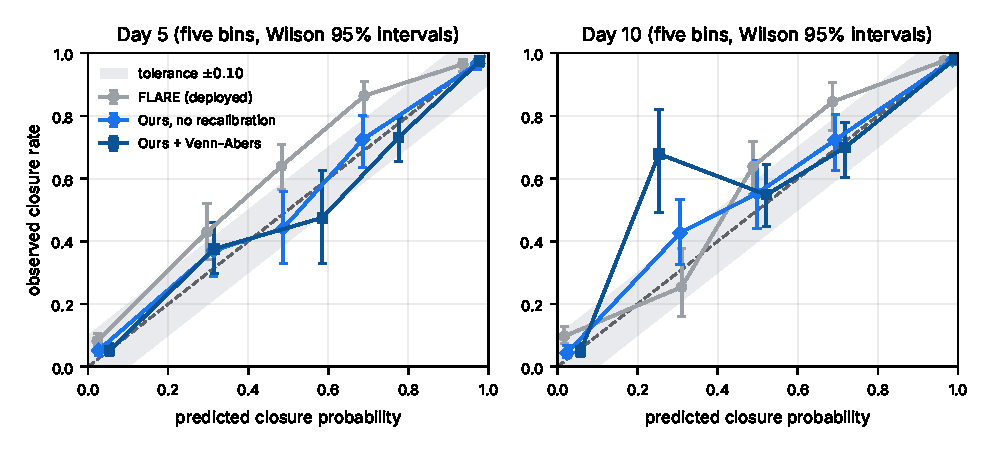
\includegraphics[width=\columnwidth]{figures/closure.pdf}
\caption{Reliability diagrams for next-observation set-closure probabilities on FLARE's ZTF test split at day 5 (left) and day 10 (right), evaluated across five equal-width bins with 95\% Wilson confidence intervals. Shaded bands denote FLARE's pre-registered $\pm0.10$ calibration tolerance and dashed diagonals indicate ideal calibration.}
\label{fig:closure}
\end{figure}

\FloatBarrier
\section{Settings Where \gamut{} Does Not Dominate}
\label{app:unfavourable}
\Cref{tab:unfavourable} catalogues every setting across the six main benchmarks and Wafer in which \gamut{} either misses bootstrap validity or is outperformed in width or class-averaged interval score by another valid method.
Six recurring mechanisms account for these cases:
\begin{enumerate}
\item \textbf{Small calibration classes at 95\%.}
On PLAsTiCC-train (smallest class 36 objects) and ECG5000 (smallest class 24 series), individual calibration folds hold only 19--40 objects of the rarest class, leaving an object-level conformal risk budget $\alpha(n_c+1)-1$ of at most one object.
Covering nearly every calibration trajectory of that class lowers $t_c(v)$ and widens the shared band through $\hat t_b=\min_c t_c(v)$, whereas MDCP and two-step CP calibrate over pooled points without an object-level guarantee (relaxing the inclusion cutoff under-covered rare validation classes, while horizon-pooled thresholds widened bands further).
\item \textbf{Point-pooled versus object-averaged coverage.}
On PLAsTiCC-train at 95\%, point-pooled SN~Ia coverage is 0.93 even though \gamut{} targets object-averaged coverage (\cref{eq:target}), because heavily cadenced objects experience slightly lower per-point coverage.
\item \textbf{Tail-distance penalties in the interval score.}
In paired object-level bootstrap comparisons of class-averaged IS, \gamut{} significantly beats/loses to two-step CP in \ISVsTwoStepGamutSixtyeight{} and \ISVsTwoStepGamutNinetyfive{} settings, max-class CP in \ISVsMaxClassGamutSixtyeight{} and \ISVsMaxClassGamutNinetyfive{}, and MDCP in \ISVsMDGamutSixtyeight{} and \ISVsMDGamutNinetyfive{} (68\%, 95\%; split-calibration \gamut{} scores \ISVsTwoStepCertSixtyeight{}, \ISVsTwoStepCertNinetyfive{}; \ISVsMaxClassCertSixtyeight{}, \ISVsMaxClassCertNinetyfive{}; \ISVsMDCertSixtyeight{}, \ISVsMDCertNinetyfive{}).
When compared post hoc against the single best valid method among all 16 candidates per setting, \gamut{} ranks first in \ISWinsGamutSixtyeight{} (68\%) and \ISWinsGamutNinetyfive{} (95\%) settings (median ratio \ISMedRatioSixtyeight{} and \ISMedRatioNinetyfive{}, maximum \ISMaxRatioNinetyfive{}), because density level sets truncate where $\hat f_c$ thins out rather than penalising miss distance linearly as IS does.
\item \textbf{In-sample reuse on sparse merged cells.}
Evaluated across \gamut{}'s merged cells, default \gamut{} leaves \MergedGamutSixtyeight{} (68\%, median shortfall \MergedDefGamutSixtyeight{}) and \MergedGamutNinetyfive{} (95\%, median shortfall \MergedDefGamutNinetyfive{}) under-covered (class, cell) pairs per setting---concentrated on rare PLAsTiCC classes (TDE, $\mu$Lens, SLSN) with 3--8 objects per fold---compared with \MergedTwoStepSixtyeight{}/\MergedTwoStepNinetyfive{} for two-step CP, \MergedMaxClassSixtyeight{}/\MergedMaxClassNinetyfive{} for max-class CP, \MergedMDCPSixtyeight{}/\MergedMDCPNinetyfive{} for MDCP, and \MergedFlareSixtyeight{}/\MergedFlareNinetyfive{} for FLARE.
Held-out threshold certification (\emph{\gamut{} (split calibration)}) reduces this to \MergedCertSixtyeight{} and \MergedCertNinetyfive{}, matching two-step CP whenever per-cell rare-class protection is prioritised.
\item \textbf{Small rare-class slices in set closure.}
In \cref{app:closure}, rare classes with 7--20 test rows using pooled validation residuals show higher Brier scores on SLSNe (days 5 and 10) and day-10 AGN/TDEs, and overall ECE matches rather than improves upon Venn--Abers-recalibrated FLARE.
\item \textbf{Conditionally valid baselines in favourable settings.}
Where Kandinsky CP or CPTC happen to pass the validity check, their bands can be slightly narrower than \gamut{}'s, but Kandinsky CP is valid in only \MainValidKandinskySixtyeight{} (68\%) and \MainValidKandinskyNinetyfive{} (95\%) of settings and CPTC in \MainValidCPTCSixtyeight{} and \MainValidCPTCNinetyfive{}, versus \MainValidGamutSixtyeight{} and \MainValidGamutNinetyfive{} for \gamut{}.
\end{enumerate}
\FloatBarrier
Every setting (benchmark, origin, level) of the six main benchmarks and Wafer in which \gamut{} is not class-valid, a latent-class-valid baseline is narrower, or a valid method has a lower class-averaged interval score. Of 42 settings: 2 not valid, 35 narrower valid baseline (method-setting pairs), 33 lower class-averaged IS by a valid method.

\begin{longtable}{lllll}
\toprule
Benchmark & Origin & Level & Event & Values \\
\midrule
\endhead
PLAsTiCC-DDF & 5 & 68\% & \gamut{} empty bands (counted as misses) & 1.4\% of points \\
PLAsTiCC-DDF & 5 & 68\% & valid MDCP lower cls-IS & 2.763 vs 2.973 \\
PLAsTiCC-DDF & 15 & 68\% & valid MDCP lower cls-IS & 2.473 vs 2.652 \\
PLAsTiCC-DDF & 30 & 68\% & valid KandinskyCP narrower & 0.764 vs 0.791 \\
PLAsTiCC-DDF & 30 & 68\% & valid KandinskyCP lower cls-IS & 1.881 vs 1.942 \\
PLAsTiCC-train & 5 & 68\% & \gamut{} empty bands (counted as misses) & 7.8\% of points \\
PLAsTiCC-train & 5 & 68\% & valid MDCP lower cls-IS & 4.213 vs 4.340 \\
PLAsTiCC-train & 15 & 68\% & \gamut{} empty bands (counted as misses) & 4.1\% of points \\
PLAsTiCC-train & 30 & 68\% & \gamut{} empty bands (counted as misses) & 1.1\% of points \\
PLAsTiCC-train & 30 & 68\% & valid CPTC lower cls-IS & 2.493 vs 2.847 \\
ECG5000 & 20 & 68\% & valid PartitionCP lower cls-IS & 1.283 vs 1.387 \\
ECG5000 & 40 & 68\% & valid KandinskyCP narrower & 0.489 vs 0.498 \\
ECG5000 & 40 & 68\% & valid KandinskyCP lower cls-IS & 1.219 vs 1.295 \\
ECG5000 & 60 & 68\% & valid KandinskyCP narrower & 0.566 vs 0.570 \\
ECG5000 & 60 & 68\% & valid LocalizedCP lower cls-IS & 1.342 vs 1.515 \\
ElecDevices & 20 & 68\% & \gamut{} empty bands (counted as misses) & 4.6\% of points \\
ElecDevices & 40 & 68\% & \gamut{} empty bands (counted as misses) & 2.3\% of points \\
ElecDevices & 60 & 68\% & valid KandinskyCP narrower & 0.867 vs 0.870 \\
StarLight & 20 & 68\% & valid MDCP narrower & 0.497 vs 0.498 \\
StarLight & 20 & 68\% & valid CPTC lower cls-IS & 0.794 vs 0.796 \\
StarLight & 40 & 68\% & valid TwoStepCP narrower & 0.301 vs 0.302 \\
StarLight & 40 & 68\% & valid KandinskyCP narrower & 0.301 vs 0.302 \\
StarLight & 40 & 68\% & valid MDCP narrower & 0.269 vs 0.302 \\
StarLight & 40 & 68\% & valid TwoStepCP lower cls-IS & 0.526 vs 0.528 \\
StarLight & 60 & 68\% & valid CPTC lower cls-IS & 0.480 vs 0.481 \\
Wafer & 20 & 68\% & valid CPTC lower cls-IS & 0.551 vs 0.553 \\
ZTF-BTS & 5 & 68\% & valid KandinskyCP narrower & 1.074 vs 1.121 \\
ZTF-BTS & 5 & 68\% & valid KandinskyCP lower cls-IS & 2.370 vs 2.464 \\
ZTF-BTS & 10 & 68\% & valid KandinskyCP narrower & 0.898 vs 0.909 \\
ZTF-BTS & 10 & 68\% & valid KandinskyCP lower cls-IS & 2.277 vs 2.413 \\
ZTF-BTS & 15 & 68\% & valid KandinskyCP lower cls-IS & 2.262 vs 2.310 \\
ZTF-BTS & 20 & 68\% & valid KandinskyCP lower cls-IS & 2.035 vs 2.054 \\
ZTF-BTS & 30 & 68\% & valid MixtureCP lower cls-IS & 1.790 vs 1.862 \\
PLAsTiCC-DDF & 5 & 95\% & valid MDCP lower cls-IS & 4.709 vs 5.183 \\
PLAsTiCC-DDF & 15 & 95\% & valid KandinskyCP narrower & 2.943 vs 3.038 \\
PLAsTiCC-DDF & 15 & 95\% & valid MDCP lower cls-IS & 4.155 vs 5.170 \\
PLAsTiCC-DDF & 30 & 95\% & valid KandinskyCP narrower & 2.240 vs 3.030 \\
PLAsTiCC-DDF & 30 & 95\% & valid CPTC lower cls-IS & 3.750 vs 4.723 \\
PLAsTiCC-train & 5 & 95\% & \gamut{} empty bands (counted as misses) & 1.5\% of points \\
PLAsTiCC-train & 5 & 95\% & \gamut{} not valid & worst 0.932 \\
PLAsTiCC-train & 5 & 95\% & valid MDCP narrower & 6.411 vs 7.233 \\
PLAsTiCC-train & 5 & 95\% & valid MDCP lower cls-IS & 6.957 vs 8.695 \\
PLAsTiCC-train & 15 & 95\% & \gamut{} empty bands (counted as misses) & 1.0\% of points \\
PLAsTiCC-train & 15 & 95\% & valid TwoStepCP narrower & 7.978 vs 8.356 \\
PLAsTiCC-train & 15 & 95\% & valid KandinskyCP narrower & 6.840 vs 8.356 \\
PLAsTiCC-train & 15 & 95\% & valid MDCP narrower & 6.777 vs 8.356 \\
PLAsTiCC-train & 15 & 95\% & valid MaxClassCP narrower & 7.981 vs 8.356 \\
PLAsTiCC-train & 15 & 95\% & valid CPTC lower cls-IS & 7.053 vs 9.738 \\
PLAsTiCC-train & 30 & 95\% & \gamut{} not valid & worst 0.926 \\
PLAsTiCC-train & 30 & 95\% & valid MixtureCP lower cls-IS & 5.384 vs 6.389 \\
ECG5000 & 20 & 95\% & valid TwoStepCP narrower & 2.126 vs 2.287 \\
ECG5000 & 20 & 95\% & valid MDCP narrower & 1.624 vs 2.287 \\
ECG5000 & 20 & 95\% & valid MaxClassCP narrower & 2.128 vs 2.287 \\
ECG5000 & 20 & 95\% & valid CPTC lower cls-IS & 2.641 vs 4.004 \\
ECG5000 & 40 & 95\% & \gamut{} empty bands (counted as misses) & 1.2\% of points \\
ECG5000 & 40 & 95\% & valid TwoStepCP narrower & 2.505 vs 2.641 \\
ECG5000 & 40 & 95\% & valid KandinskyCP narrower & 1.216 vs 2.641 \\
ECG5000 & 40 & 95\% & valid MDCP narrower & 1.658 vs 2.641 \\
ECG5000 & 40 & 95\% & valid MaxClassCP narrower & 2.506 vs 2.641 \\
ECG5000 & 40 & 95\% & valid PartitionCP lower cls-IS & 2.356 vs 4.164 \\
ECG5000 & 60 & 95\% & \gamut{} empty bands (counted as misses) & 1.1\% of points \\
ECG5000 & 60 & 95\% & valid TwoStepCP narrower & 2.330 vs 3.303 \\
ECG5000 & 60 & 95\% & valid KandinskyCP narrower & 1.475 vs 3.303 \\
ECG5000 & 60 & 95\% & valid MDCP narrower & 2.288 vs 3.303 \\
ECG5000 & 60 & 95\% & valid MaxClassCP narrower & 2.331 vs 3.303 \\
ECG5000 & 60 & 95\% & valid CPTC lower cls-IS & 2.850 vs 5.125 \\
StarLight & 20 & 95\% & valid MDCP narrower & 1.237 vs 1.239 \\
StarLight & 40 & 95\% & valid MDCP narrower & 0.707 vs 0.761 \\
StarLight & 60 & 95\% & valid TwoStepCP narrower & 0.710 vs 0.713 \\
StarLight & 60 & 95\% & valid KandinskyCP narrower & 0.711 vs 0.713 \\
StarLight & 60 & 95\% & valid TwoStepCP lower cls-IS & 1.047 vs 1.049 \\
Wafer & 20 & 95\% & valid CPTC lower cls-IS & 1.440 vs 1.450 \\
ZTF-BTS & 5 & 95\% & valid KandinskyCP narrower & 2.647 vs 2.910 \\
ZTF-BTS & 5 & 95\% & valid MDCP lower cls-IS & 4.404 vs 4.694 \\
ZTF-BTS & 10 & 95\% & valid KandinskyCP narrower & 2.241 vs 2.481 \\
ZTF-BTS & 10 & 95\% & valid KandinskyCP lower cls-IS & 4.405 vs 4.622 \\
ZTF-BTS & 15 & 95\% & valid CPTC lower cls-IS & 3.902 vs 4.268 \\
ZTF-BTS & 20 & 95\% & valid CPTC lower cls-IS & 3.693 vs 4.027 \\
ZTF-BTS & 30 & 95\% & valid KandinskyCP narrower & 1.502 vs 1.584 \\
ZTF-BTS & 30 & 95\% & valid CPTC lower cls-IS & 3.322 vs 3.736 \\
\bottomrule
\end{longtable}

\FloatBarrier

\FloatBarrier
\section{Development History and Test-Set Exposure}
\label{app:history}
To maintain transparent scientific reporting, we document below which design decisions were informed by main-benchmark outputs prior to freezing the codebase for the held-out evaluations:
\begin{itemize}
\item Data-adaptive horizon-cell merging was motivated by sparse-cell behaviour on PLAsTiCC-train and tuned on nested validation folds.
\item The dual-resolution evaluation grid (adding 49 local points per hypothesis) was introduced after ElectricDevices runs revealed narrow intervals falling between coarse grid points; the identical grid was applied to all grid-evaluated baselines.
\item Extending standardised residual support from $[-12,12]$ to $[-60,60]$ followed 95\% ElectricDevices tail truncations.
\item A horizon-pooled threshold variant was inspected on a single ECG5000 fold and discarded.
\item Smoothing bandwidth ($\times 2$ Silverman) and finite-sample CRC adjustments were selected purely on nested validation folds.
\item Main-text reporting shifted from fixed worst-class tolerances to object-level bootstrap intervals (\cref{tab:validity} reports both) and from class-averaged IS to band width matching \cref{prop:oracle} (\cref{app:unfavourable} reports full IS comparisons).
\item Bootstrap random number generators were seeded deterministically per setting and method so Monte-Carlo intervals remain invariant to the ordering of evaluated baselines.
\end{itemize}
Both pre-registered held-out PLAsTiCC WFD benchmarks (\cref{app:held}) were executed strictly after freezing all above choices.

\FloatBarrier
\section{Pre-Registered Experiment Plan and Outcomes}
\label{app:plan}
\Cref{tab:plan} audits every hypothesis and experimental block recorded in our initial study plan prior to running the main benchmarks, alongside the separate registrations in \cref{app:held,app:closure}; preliminary alternatives (unions of class intervals, unweighted density level sets, and HPD mass thresholds) were omitted after preliminary validation checks.
\FloatBarrier
{\scriptsize
\begin{longtable}{p{1.6cm}p{4.2cm}p{9.2cm}}
\caption{Every claim and block registered in the experiment plan, with its outcome.}
\label{tab:plan}\\
\toprule
Registered & Criterion & Outcome \\
\midrule
\endfirsthead
\toprule
Registered & Criterion & Outcome \\
\midrule
\endhead
C1 validity & Worst class $\ge$ nominal $-0.02$/$-0.015$ on $\ge$6 benchmarks at every origin & Not met as registered: 85\% (68\%) and 90\% (95\%) of settings under this tolerance; 100\% and 90\% under the bootstrap rule used in the text \\
C2 efficiency & Smallest class-averaged IS and width among valid methods on $\ge$6 benchmarks & Not met: lowest class-averaged IS in 3/20 and 5/20 settings; paired bootstrap significantly better in 3/20 and 5/20, worse in 13/20 and 14/20. Width: shorter than the always-valid baselines by 27\% (68\%) and 20\% (95\%) on average, but wider than MDCP in 7/20 settings at 95\% \\
C3 components & Removing any of C1/C2/C3 degrades validity or IS on most benchmarks & Met for C2 and C3 (validity or width, \cref{tab:ablation}); not met for C1 on the real benchmarks (+3--4\% width, validity at 95\% 90\% $\to$ 85\%), met on the synthetic family \\
C4 theory & Synthetic: observed gap matches Prop.~1; \gamut{} near the oracle length & Met: Prop.~1 within 0.026; \gamut{} 2.3\%/7.5\% longer than the oracle band \\
C5 robustness & Coverage under degraded posteriors, prior shift, small calibration sets & Partly run: posterior temperature distortion (synthetic $\kappa$) only. Label-noise posteriors, calibration subsampling and the train$\to$DDF prior shift (block B6) were not run; the strict split and the held-out set were added instead \\
B1 paired IS test & Paired object-level bootstrap of class-averaged IS vs the best valid baseline & Run after review (\texttt{scripts/is\_bootstrap.py}): significantly better in 3/20/5/20, worse in 13/20/14/20 \\
B4 grid & Bandwidth $\times\{0.5,1,2\}$ and other hyperparameters on validation folds & Run with bandwidth $\times\{1,2,4\}$ (the default moved to $\times2$), plus dual iterations and fixed lead bins; the other registered values as planned \\
central-interval ablation (not adopted) & Valid at every origin and level of PLAsTiCC chunk 03 and lower class-averaged IS than every valid baseline in most settings & Not met: valid in 100\% and 33\% of the chunk-03 settings, IS better/worse in 3/0 and 1/2; not adopted \\
B0, B2, B3, B5, B7, B8 & Observation, ablations, synthetic, per-horizon curves, runtime, closure probability & Run as registered (B8 with its own registration, \cref{app:closure}) \\
\bottomrule
\end{longtable}}
\FloatBarrier

\FloatBarrier
\section{Limitations}
\label{app:limits}
\begin{itemize}
\item \textbf{Taxonomy and labels.} Class validity holds for the classes and labels of the calibration set. A class absent from the taxonomy, or labelled unreliably, is not protected. ECG5000 labels come from automated annotation, so on that benchmark ``class'' is a noisy proxy.
\item \textbf{Exchangeability.} We assume that objects of a class are exchangeable between calibration and test. On ZTF and PLAsTiCC this mirrors FLARE's own protocol. Spectroscopically labelled calibration objects can be selected on brightness, which correlates with the forecast target. If test objects are selected differently, coverage can drift, for every method. A survey whose class mix or selection changes over time needs recalibration. Class-conditional validity is invariant to changes of class priors alone \citep{podkopaev2021distribution}.
\item \textbf{Finite samples.} The default \gamut{} fits its weights, residual laws and temperature on the calibration objects and has no finite-sample guarantee; the uniform-convergence bound in \cref{app:proofs} is too loose to help at our class sizes. \gamut-cert is valid in finite samples under a strict split, but it is conservative when a class has few objects. A class with fewer than $1/\alpha-1$ certification objects in a horizon cell gets no guarantee there and is left out of that cell's threshold; at 95\% on small calibration sets these are exactly the rare classes.
\item \textbf{Horizon cells.} With few calibration objects, the merging rule coarsens the horizon cells, at the extreme to a single cell. Validity is then per merged cell, not per FLARE bin. The realised cells are listed in \cref{app:cert}, and per-bin coverage is checked by bootstrap.
\item \textbf{Empty bands.} A level set can be empty at an input whose class hypotheses are all diffuse; the length-optimal band then gives up that point. On ZTF this happens for at most 0.01\% of future points. Elsewhere it is not negligible: at 68\% up to 7.8\% of points on PLAsTiCC-train, 4.6\% on ElectricDevices and 1.4\% on PLAsTiCC-DDF, and at 95\% up to 1.5\% on PLAsTiCC-train and 1.2\% on ECG5000 (\cref{app:unfavourable}). We count empty bands as misses. A deployment that needs a band at every point can fall back to the posterior-mixture band there, which we did not evaluate.
\item \textbf{Discrete targets.} On ElectricDevices 52--59\% of the targets are exactly zero, so $Y$ has no Lebesgue density there, against the assumption of \cref{prop:oracle}, and band lengths depend on the evaluation grid near zero.
\item \textbf{Length on a grid.} Coverage is computed from the exact score, and length on a grid of 400 uniform points plus 49 points around every class hypothesis. A band narrower than the finest grid cell is counted as empty, and hence as a miss, which is conservative.
\item \textbf{Unions of intervals.} When class forecasts disagree, the band can be a union of intervals. This is informative (``either it fades like a SN~Ia or stays bright like an SLSN''). In our benchmarks the hull is at most 2\% longer than the union on average, so the bands are almost always single intervals.
\item \textbf{Shared base models.} We changed only the calibration step. A better base forecaster or classifier narrows every method's bands. For compute reasons we used a learning rate of 0.05 (ZTF) or 0.1 (other benchmarks) instead of FLARE's 0.02, the same for all methods.
\item \textbf{UCR normalisation.} The archive z-normalises each series over its full length, which leaks scale information into the prefix. All methods see the same inputs, so their comparison is unaffected, but absolute widths on UCR are optimistic.
\item \textbf{Test-set exposure and the validity rule.} Several design choices (adaptive cells, the support of the residual laws, the evaluation grid, the validity rule) were revised after test results had been seen (\cref{app:history}). The pre-registered held-out set (\cref{app:held}) bounds this effect, but it is one benchmark under the cross-fitted protocol, with six settings. The bootstrap rule tests each class separately, without a multiplicity correction, and it has little power for classes with few objects: a class of 20 objects is flagged only when its coverage is far below nominal. Both points make the reported validity rates optimistic, for \gamut{} and for every baseline alike.
\item \textbf{Same-family review.} The internal reviews of this work were done by models of the same family as the executor (\texttt{review\_independence: same-family}); they are not independent peer review.
\end{itemize}



\end{document}
